\documentclass[12pt, letterpaper]{article}
\usepackage[utf8]{inputenc}
\usepackage{amsthm}
\usepackage{amsmath}
\usepackage{bm}
\usepackage{cancel}
\usepackage[ruled, vlined,]{algorithm2e}
\usepackage{graphicx}
\usepackage[upgreek]{mathastext}
\usepackage{eucal}
\usepackage{subcaption}
\usepackage{hyperref}
\usepackage{flafter} %avoids that figures are floated before they were defined, i.e. before section title
\usepackage{listings}
\usepackage{booktabs}% pandas.to_latex() \toprule, \bottomrule, 
\usepackage[dvipsnames,table,xcdraw]{xcolor}
\usepackage{imakeidx}
\usepackage{systeme}
\usepackage{xcolor}
\usepackage{listings}
\usepackage{subcaption}
\usepackage{xparse}

\makeindex
\theoremstyle{definition}
\newtheorem{definition}{Definition}[section] 
 
\newcommand{\R}{\mathbb{R}} 
\newcommand{\E}{{\rm I\kern-.3em E}}

\newcommand{\Var}{\mathrm{Var}}
\newcommand{\Cov}{\mathrm{Cov}}
\newcommand{\X}{\mathrm{\mathbf{X}}}
\newcommand{\w}{\mathrm{\mathbf{w}}}
\newcommand{\I}{\mathrm{\mathbf{I}}}
\newcommand{\hS}{\mathrm{\hat{\mathbf{\Sigma}}}}
\newcommand{\hsi}{\mathrm{\hat{\mathbf{\Sigma}}}^{-1}}
\newcommand{\si}{\mathbf{\Sigma}^{-1}}
\newcommand{\y}{\mathbf{y}}
\newcommand{\be}{\mathbf{\beta}}
\newcommand{\e}{\mathbf{\epsilon}}
\newcommand{\al}{\mathbf{\alpha}}
\newcommand{\hbe}{\hat{\mathbf{\beta}}}
\newcommand{\Tr}{\mathbf{Tr}}
\newcommand{\x}{\mathbf{x}}
\newcommand{\hmu}{\hat{\mu}}
\usepackage{mathtools} 
\DeclarePairedDelimiter\autobracket{(}{)}
\newcommand{\br}[1]{\autobracket*{#1}}
\newcommand{\hpi}{\hat{\pi}}
\newcommand{\hs}{\hat{\sigma}^2}
\newcommand{\ssq}{\sigma^2}
\newcommand{\sz}{\sigma(z)}
\newcommand{\dsz}{\sigma'(z)}
\newtheorem{theorem}{Theorem}
\newcommand{\inv}{\mathrm{\left( \X^T\X\right)^{-1}}} 
\newcommand{\HM}{\mathrm{\inv\X^T}} 
\newcommand{\pr}{\mathrm{\partial}} 
\newcommand{\hb}{\mathrm{\hat{\mathbf{\beta}}}} 
\newcommand{\mb}{\mathrm{\mathbf}}
\newcommand\norm[1]{\left\lVert#1\right\rVert}
%\newcommand\br[1]{\left(#1\right)}
%\newcommand\sbr[1]{\left[#1\right]}

\newcommand{\argmax}[1]{\underset{#1}{\operatorname{arg}\,\operatorname{max}}\;}
\newcommand{\argmin}[1]{\underset{#1}{\operatorname{arg}\,\operatorname{min}}\;}
\usepackage{amssymb}
 
\let\ti\textit
\let\tb\textbf
\let\cd\lstinline
 
\definecolor{deepblue}{rgb}{0,0,0.5}
\definecolor{deepred}{rgb}{0.6,0,0}
\definecolor{deepgreen}{rgb}{0,0.5,0}
\DeclareFixedFont{\ttb}{T1}{txtt}{bx}{n}{10} % for bold
\DeclareFixedFont{\ttm}{T1}{txtt}{m}{n}{10}  % for normal
 
 
 
\begin{document}
% Python style for highlighting
\lstdefinestyle{customc}{
belowcaptionskip=1\baselineskip,
breaklines=true,
%frame=L,
xleftmargin=\parindent,
language = Python,
showstringspaces=false,
basicstyle=\footnotesize\ttfamily,
keywordstyle=\bfseries\color{blue!85!black},
commentstyle=\itshape\color{gray},
identifierstyle=\color{black},
stringstyle=\color{red},
  numbers=left,                    				% where to put the line-numbers; possible values are (none, left, right)
  numbersep=5pt,                   			% how far the line-numbers are from the code
  numberstyle=\tiny\color{gray}, % the style that is used for the line-numbers
  stepnumber=1,
  tabsize=4,
}
\lstdefinestyle{customasm}{
  belowcaptionskip=1\baselineskip,
  frame=L,
  %xleftmargin=\parindent,
  language=[x86masm]Assembler,
  basicstyle=\footnotesize\ttfamily,
  commentstyle=\itshape\color{purple!40!black},
  stepnumber=1,
   tabsize=4,
}
\lstset{escapechar=@,style=customc}

\title{Machine learning notes}
\author{Francesco Boi}
\date{\vspace{-5ex}}
\maketitle
\numberwithin{equation}{section}
\numberwithin{figure}{section}
\tableofcontents
\section{Preliminary definitions}
\subsection{Matrix properties and definitions}
\subsubsection{Trace of a matrix}
\index{Trace of a matrix}
\label{trace}
The \textbf{trace} of a square matrix $\mathbf{A}$, denoted as $\Tr(\mathbf{A})$ is the sum of diagonal elements:
\begin{equation}
\Tr(\mathbf{A}) = \sum_{d=1}^p A_{dd}
\end{equation}
It follows that $Tr(\mathbf{I_d}) = p$.
Also $\Tr(\mathbf{AB}) = \Tr(\mathbf{AB})$ and $\Tr(\x^T\x) = \x^T\x$ the latter being a scalar.

\subsubsection{Exponential matrices}
\label{ExponentialMatrices}
\index{Exponential Matrices}
\begin{definition}{\tb{Exponential matrix}} The matrix exponential is a matrix function on square matrices analogous to the ordinary exponential function. Let $X$ be an $N\times N$ real or complex matrix. Its exponential denoted by $e^X$ is the $N \times N$ matrix given by the power series:
\begin{equation}
e^X = \sum_{k=0}^\infty \frac{1}{k!} X^k
\end{equation}
where $X^0 = I_N$.
\end{definition}

\subsubsection{Similar matrices}
\label{MatrixSimilarity}
\index{Similar matrices}
\begin{definition}{\tb{Similar matrices}}In linear algebra, two $N\times N$ matrices $A$ and $B$ are called \tb{similar} if there exists a $N\times N$ invertible matrix $P$ such that:
\begin{equation}
B = P^{-1}AP
\end{equation}	
\end{definition}
\index{Similar matrices}

\paragraph{\tb{Example}} Similar matrices represent the same linear map under two (possibly) different bases, with $P$ being the change of basis matrix. For example, a rotation around an axis not aligned with the coordinate axis might be difficult to express.  If the axis of rotation is aligned with the positive $z$-axis, then the rotation is simply $S =\begin{bmatrix}\cos \theta &-\sin \theta &0\\\sin \theta &\cos \theta &0\\0&0&1\end{bmatrix}$. So in these new space such a rotation is $y' = Sx'$ where $x'$ and $y'$ are respectively the points before and after the rotation in the new more convenient space. 
In the original space the transformation is $y = Tx$. Then assuming $P$ is the change of base matrix, $T$ can be found as $y' = P y = PTx= S x' \Rightarrow T = P^{-1} S P$.

\subsubsection{Diagonalizable matrices}
\index{Diagonalizable matrices}
\begin{definition}{\tb{Diagonalizable matrices}} In linear algebra, a matrix is called \tb{diagonalizable} if it is similar \autoref{MatrixSimilarity} to a diagonal matrix, i.e., if there exists an invertible matrix $P$ and a diagonal matrix $D$ such that $P^{-1}AP =D$.
\end{definition}

\subsection{Eigenvalue decomposition}
\index{Eigenvalue}
\index{Eigenvector}
\begin{definition}{\tb{Eigenvalues and eigenvector}}
A (non-zero) vector $\vec{v}$ is an \tb{eigenvector} of a square matrix $A \in \CMcal{R}^{N\times N}$ if it satisfies the linear equation:
\begin{equation}
A\vec{v} = \lambda \vec{v}
\label{eigenvector}
\end{equation}
where $\lambda$ is a scalar, termed \tb{eigenvalue} associated to the eigenvector $\vec{v}$. 
\end{definition}
That is, the eigenvectors are the vectors that the linear transformation A merely elongates or shrinks, and the amount that they elongate/shrink by is the eigenvalue.

From this we get an equation for the eigenvalues.
\begin{definition}{\tb{characteristic polynomial} and \tb{characteristic equation}}
\begin{equation}
p(\lambda) = \det\br{A - \lambda I}  = 0
\end{equation}
$p(\lambda)$ is called \tb{characteristic polynomial} and the equation \tb{characteristic equation}.
\end{definition}
$p(\lambda)$ is a $N$-th order polynomial equation in $\lambda$. The set of solution is called \tb{spectrum of $A$}.  
$p(\lambda)$ can be refactored as:
\begin{equation}
p(\lambda) = \br{\lambda - \lambda_1}^{n_1} \br{\lambda - \lambda_2}^{n_2}\cdots \br{\lambda - \lambda_\lambda}^{n_\lambda}
\end{equation}
where $n_i$ is termed the \tb{algebraic multiplicity of the eigenvalue $\lambda_i$}. The number of distinct eigenvalue is $0\le N_\lambda\le N$.

For each eigenvalue we have a specific eigenvalue equation:
\begin{equation}
\br{A-\lambda_i I} \vec{v}= 0
\end{equation}
and there will be $0\le m_i \le n_i$ linearly independent solutions to each eigenvalue equation. The term $m_i$ is termed \tb{geometric multiplicity of $\lambda_i$}, with $m_i \le n_i$, the algebraic multiplicity.

\subsection{Decomposition}
\index{Eigenvalues decomposition}
Eigendecomposition or sometimes spectral decomposition is the factorization of a matrix into a canonical form, whereby the matrix is represented in terms of its eigenvalues and eigenvectors. Only diagonalizable matrices can be factorized in this way. 

Let $A$ be a $N\times N$ square matrix with $N$ linearly independent eigenvectors $q_i$ where $i=1, \cdots, n$. Then $A$ can be factorized as 
\begin{equation}
A = Q \Lambda Q^{-1}
\end{equation}
where $Q$ is  the square $n\times n$ matrix whose $i-th$ column is the eigenvector $q_i$ of $A$, and $\Lambda$ is the diagonal matrix whose diagonal elements are the eigenvalues. The $q_i$ eigenvector are generally normalized but they need not be: the magnitudes of the eigenvectors in $Q$ get cancelled by $Q^{-1}$:
\begin{equation}
A\vec{v} = \lambda \vec{v}\Rightarrow AQ = Q\Lambda \Rightarrow A = Q\Lambda Q^{-1}
\end{equation}
The eigenvalue decomposition gives an easy way to compute power of matrices or exponential matrices:
\begin{equation}
\begin{aligned}
A^{-1} &= Q\Lambda^{-1}Q^{-1}\\
A^n    &=  Q\Lambda^{n}Q^{-1}\\
e^A    &=  Q\left[diag\br{e^\lambda_{ii}}\right]Q^{-1}\\
\end{aligned}
\end{equation}

\subsection{Singular Value Decomposition}
\label{SVD}
It is a factorization of a real or complex matrix that generalizes of the eigendecomposition of a square normal matrix to any $m\times n$ matrix. Given a $m\times n$ real or complex matrix $M$,
\begin{equation}
M = U \Sigma V^*
\end{equation}
where $U$ is a $m \times m$ real or complex unitary matrix, $\Sigma$ is a $m \times n$ rectangular diagonal matrix with non-negative real numbers termed \tb{singular values} on the diagonal and $V$ is a real or complex $n\times n$ unitary matrix. If $M$ is real, $U$ and $V*=V$ are orthonormal matrices, i.e., $U^TU=I$ and $V^TV=I$.

The number of non-zero singular values is equal to the rank of $M$. The column of $U$ and $V$ are called \tb{left singular vectors} and \tb{right singular vectors}. The SVD is not unique. However, it is always possible to choose the decomposition in order to have the singular values in descending order: $\sigma_1 \ge \sigma_2 \ge \sigma_3 \cdots$. In this way $\Sigma$ is uniquely determined, but \tb{not} $U$ and $V$.

In the special case when $M$ is an $m \times m$ real square matrix, the matrices $U$ and $V*$ can be chosen to be real $m \times m$ matrices too. In that case, "unitary" is the same as "orthonormal". Then, interpreting each such matrix $A$ as the linear transformation $x \rightarrow Ax$ of the space $\CMcal{R}^m$, the matrices $U$ and $V*$ represent rotations or reflection of the space, while $\Sigma$ represent the scaling of each coordinate $x_i$ by the factor $\sigma_i$. Thus the SVD decomposition breaks down any invertible linear transformation of $R^m$ into a composition of three geometrical transformations: a rotation or reflection ($V^*$), followed by a coordinate-by-coordinate scaling ($\Sigma$), followed by another rotation or reflection ($U$).

The singular values can be interpreted as the magnitude of the semiaxis of an ellipse in 2D. Singular values encode magnitude of the semiaxis, while singular vectors encode direction. the columns of $U$, $U^*$, $V$, and $V^*$ are orthonormal bases. When the $\mathbf {M}$ is a normal matrix, $U$ and $V^*$ reduce to the unitary used to diagonalize $\mathbf {M}$. However, when 
$\mathbf {M}$  is not normal but still diagonalizable, its eigendecomposition and singular value decomposition are distinct.


\subsubsection{Relationship with eigendecomposition}
\label{SVDEigenDec}
\begin{equation}
\begin{aligned}
M^*M &= V \Sigma^* U^*U \Sigma V^* = V\Sigma^* \Sigma V^*\\
MM^* &= U \Sigma V^*V \Sigma^* U^* = U \Sigma \Sigma^* U^*
\end{aligned}
\end{equation}
The right-hand sides of these relations describe the eigenvalue decompositions of the left-hand sides. The columns of $V$ (right-singular vectors) are eigenvectors of $M^*M$. The columns of $U$ (left-singular vectors) are eigenvectors of $MM^*$. The non-zero elements of $\Sigma$ (non-zero singular values) are the square roots of the non-zero eigenvalues of $M^*M$ or $MM^*$.

Defining the \tb{matrix of principal component variables}
\begin{equation}
Z = U\Sigma
\end{equation}
we can find $Z$ from the eigenvalue-decomposition of $M^*M = W D W^{-1}$.$\Sigma$ is found as explained above. If $W$ is chosen to be orthogonal, then we can set $U=W$, hence we have $Z$.

\subsection{Expectation}
\index{Expectation}
\begin{definition}{\textbf{Expectation}}
Let $X$ be a random variable with a finite number of outcomes $x_1, x_2, \cdots, x_k$ occurring respectively with probabilities $p_1, p_2, \cdots, p_k$. The expectation value is the summation of each outcome times its probability.
\begin{equation}
\E\left[ X\right]= \sum_k x_k \cdot p_k
\end{equation}

In case of an infinite number of outcomes the summation is replaced with the integral:
\begin{equation}
\E\left[ X\right]= \int x \cdot p\left(x \right) dx
\end{equation}
\end{definition}

\href{https://stats.stackexchange.com/a/72614/238980}{As explained here}, when many random variables are involved, and there is no subscript in the $E$ symbol, the expected value is taken with respect to their joint distribution:

$$E[h(X,Y)] = \int_{-\infty}^\infty \int_{-\infty}^\infty h(x,y) f_{XY}(x,y) \, dx \, dy$$


When a subscript is present, in some cases it tells us on which variable we should condition. So

$$E_X[h(X,Y)] = E[h(X,Y)\mid X] = \int_{-\infty}^\infty h(x,y) f_{h(X,Y)\mid X}(h(x,y)\mid x)\,dh  $$

...But in other cases, it tells us which density to use for the "averaging"

$$E_X[h(X,Y)] = \int_{-\infty}^\infty h(x,y) f_{X}(x) \, dx $$


\subsection{Variance}
\index{Variance}
\label{Variance}
\begin{definition}{\textbf{Variance}}
The variance of a random variable $X$ is the expected value of the squared deviation from the mean of $X$:
\begin{equation}
Var\left( X\right) = E\left[ \left( X - \mu \right)^2\right] 
\end{equation}

Variance can be expressed in another way recalling $\mu = E\left[ X\right]$ and using the linearity property:
\begin{equation}
\begin{aligned}
	Var\left( X\right) &= E\left[ \left( X - \mu \right)^2\right] = E\left[ \left( X - E\left[ X\right] \right)^2\right] =\\
	&= E\left[ X^2 - 2\cdot X \cdot E\left[ X\right] + E\left[ X\right] ^2\right]\\
	&= E\left[ X^2\right] - 2\cdot E\left[X \cdot \mu \right]+ E\left[\mu^2\right]\\
	&= E\left[ X^2\right] - 2\cdot \mu \cdot E\left[X\right]+\mu^2 \\
	&= E\left[ X^2\right] - \mu^2 = E\left[ X^2\right] - E\left[ X\right] ^2 \\
\end{aligned}
\end{equation}

\end{definition}

\subsection{Median}
\index{Median}
\begin{definition}{\textbf{Median}}
For any probability distribution on the real line $\R$ with cumulative distribution function $F$, regardless of whether it is any kind of continuous probability distribution, in particular an absolutely continuous distribution (which has a probability density function), or a discrete probability distribution, a median is by definition any real number $m$ that satisfies the inequalities:
\begin{align}
P(x\le m) \ge \frac{1}{2} \quad \text{and} \quad P(x\le m) \ge \frac{1}{2}\\
\end{align}

or equivalently the inequalities
\begin{equation}
\int_{- \infty}^{m} F(x) dx \ge  \frac{1}{2} \quad \text{and} \quad \int_{m}^{\infty} F(x) dx \ge  \frac{1}{2} 
\end{equation}
\end{definition}

\subsection{Median as the minimizer of $L_1$ norm}
%\index{Preliminary definitions!Median as the minimizer of $L_1$ norm}
\label{medianMin}
Assume that $S$ is a finite set, with say $k$ elements. Line them up in order, as $s_1<s_2<\cdots <s_k$.  

If $k$ is even there are (depending on the exact definition of median) many medians. $|x-s_i|$ is the \textit{distance} between $x$ and $s_i$, so we are trying to minimize the sum of the distances. For example, we have $k$ people who live at various points on the $x$-axis. We want to find the point(s) $x$ such that the sum of the travel distances of the $k$ people to $x$ is a minimum.

Imagine that the $s_i$ are points on the $x$-axis. For clarity, take $k=7$. Start from well to the left of all the $s_i$, and take a tiny step, say of length $\epsilon$, to the right. Then you have gotten $\epsilon$ closer to every one of the $s_i$, so the sum of the distances has decreased by $7\epsilon$. 

Keep taking tiny steps to the right, each time getting a decrease of $7\epsilon$. This continues until you hit $s_1$. If you now take a tiny step to the right, then your distance from $s_1$ increases by $\epsilon$, and your distance from each of the remaining $s_i$  decreases by $\epsilon$. So there is a decrease of $6\epsilon$, and an increase of $\epsilon$, for a net decrease of $5\epsilon$ in the sum. 

This continues until you hit $s_2$. Now, when you take a tiny step to the right, your distance from each of $s_1$ and $s_2$ increases by $\epsilon$, and your distance from each of the five others decreases by $\epsilon$, for a net decrease of $3\epsilon$.

This continues until you hit $s_3$. The next tiny step gives an increase of $3\epsilon$, and a decrease of $4\epsilon$, for a net decrease of $\epsilon$.

This continues until you hit $s_4$. The next little step brings a total increase of $4\epsilon$, and a total decrease of $3\epsilon$, for an increase of $\epsilon$. Things get even worse when you travel further to the right. So the minimum sum of distances is reached at $s_4$, the median.

The situation is quite similar if $k$ is even, say $k=6$. As you travel to the right, there is a net decrease at every step, until you hit $s_3$. When you are between $s_3$ and $s_4$, a tiny step of $\epsilon$ increases your distance from each of $s_1$, $s_2$, and $s_3$ by $\epsilon$. But it decreases your distance from each of the three others, for no net gain. Thus any $x$ in the interval from  $s_3$ to $s_4$, including the endpoints, minimizes the sum of the distances. 

In the even case, Some people prefer to say that any point between the two "middle" points is a median. So the conclusion is that the points that minimize the sum are the medians. Other people prefer to define the median in the even case to be the average of the two "middle" points. Then the median does minimize the sum of the distances, but some other points also do.

\textbf{In formulas} consider two $x_i$'s $x_1$ and $x_2$, with $x_2>x_1$
\begin{itemize}
\item \begin{equation}\begin{aligned}
&x_1\leq a\leq x_2
\\ &\sum_{i=1}^{2}|x_i-a|=|x_1-a|+|x_2-a|=a-x_1+x_2-a=x_2-x_1
\end{aligned}\end{equation}
\item \begin{equation}\begin{aligned}
&a < x_1
\\&\sum_{i=1}^{2}|x_i-a|=x_1-a+x_2-a=x_1+x_2-2a\ge x_1+x_2-2x_1\\=&x_2-x_1
\end{aligned}\end{equation}
\item \begin{equation}\begin{aligned}
&a\ge x_2
\\&\sum_{i=1}^{2}|x_i-a|&=-x_1+a-x_2+a=-x_1-x_2+2a\ge -x_1-x_2+2x_2=\\
&=x_2 - x_1
\end{aligned}
\end{equation}

\end{itemize}


$\implies$for any two $x_i$'s the sum of the absolute values of the deviations is minimum when $x_1\leq a\leq x_2$ or $a\in[x_1,x_2]$.

When $n$ is odd,
\begin{equation}
\begin{aligned}
\sum_{i=1}^n\left|x_i-a\right|=\left|x_1-a\right|&+\left|x_2-a\right|+\cdots+\left|x_{\tfrac{n-1}{2}}-a\right| + \left|x_{\tfrac{n+1}{2}}-a\right|+\\
&+ \left|x_{\tfrac{n+3}{2}}-a\right|+ \cdots+\left|x_{n-1}-a\right|+\left|x_n-a\right|
\end{aligned}
\end{equation}
consider the intervals $[x_1,x_n], [x_2,x_{n-1}], [x_3,x_{n-2}], \ldots, \left[x_{\tfrac{n-1}{2}}, x_{\tfrac{n+3}{2}}\right]$. If $a$ is a member of all these intervals. i.e, $\left[x_{\tfrac{n-1}{2}},x_{\tfrac{n+3}{2}}\right],$

using the above theorem, we can say that all the terms in the sum except $\left|x_{\tfrac{n+1}{2}}-a\right|$ are minimized. So
\begin{equation}
\begin{aligned}
\sum_{i=1}^n|x_i-a|&=(x_n-x_1)+(x_{n-1}-x_2)+(x_{n-2}-x_3)+\cdots +\\
& +\left(x_{\tfrac{n+3}{2}}-x_{\tfrac{n-1}{2}}\right) + \left|x_{\tfrac{n+1}{2}}-a\right| = \left|x_{\tfrac{n+1}{2}}-a \right|+\text{costant}
\end{aligned}
\end{equation}

To minimize also the term $\left|x_{\tfrac{n+1}{2}}-a \right|$ it is clear we have to choose $a=x_{\tfrac{n+1}{2}}$ to get $0$ but this is the definition of the median.

$\implies$ When $n$ is odd,the median minimizes the sum of absolute values of the deviations.

When $n$ is even,
\begin{equation}
\begin{aligned}
\sum_{i=1}^n|x_i-a|=|x_1-a|+|x_2-a|+\cdots+\\
+|x_{\tfrac{n}{2}}-a|+|x_{\tfrac{n}{2}+1}-a|+\\
 \cdots+|x_{n-1}-a|+|x_n-a|
\end{aligned}
\end{equation}
If $a$ is a member of all the intervals $[x_1,x_n], [x_2,x_{n-1}], [x_3,x_{n-2}]$, $\ldots$, $\left[x_{\tfrac{n}{2}},x_{\tfrac{n}{2}+1}\right]$, i.e, $a\in\left[x_{\tfrac{n}{2}},x_{\tfrac{n}{2}+1}\right]$,

\begin{equation}
\begin{aligned}
&\sum_{i=1}^n|x_i-a|=(x_n-x_1)+(x_{n-1}-x_2)+(x_{n-2}-x_3)+\cdots + \\
&+\left(x_{\tfrac{n}{2}+1}-x_{\tfrac{n}{2}}\right)
\end{aligned}
\end{equation}

$\implies$ When $n$ is even, any number in the interval $[x_{\tfrac{n}{2}},x_{\tfrac{n}{2}+1}]$, i.e, including the median, minimizes the sum of absolute values of the deviations. For example consider the series:$2, 4, 5, 10$, median, $M=4.5$.

$$
\sum_{i=1}^4|x_i-M|=2.5+0.5+0.5+5.5=9
$$
If you take any other value in the interval $\left[x_{\tfrac{n}{2}},x_{\tfrac{n}{2} + 1} \right] =[4,5]$, say $4.1$
$$
\sum_{i=1}^4|x_i-4.1|=2.1+0.1+0.9+5.9=9
$$

Taking for example $4$ or $5$ yields the same result:
$$
\sum_{i=1}^4|x_i-4|=2+0+1+6=9
$$

$$
\sum_{i=1}^4|x_i-5|=3+1+0+5=9
$$

This is because when summing the distance from $a$ to the two middle points, you end up with the distance between them: $a-x_{\tfrac{n}{2}}+(x_{\tfrac{n}{2}+1}-a) = x_{\tfrac{n}{2}+1}-x_{\tfrac{n}{2}}$

For any value outside the interval $\left[x_{\tfrac{n}{2}},x_{\tfrac{n}{2}+1}\right]=[4,5]$, say $5.2$
$$
\sum_{i=1}^4|x_i-5.2|=3.2+1.2+0.2+4.8=9.4
$$

%%%%%%%%%
\index{Correlation}
\subsection{Correlation}
In statistics, dependence or association is any statistical relationship, whether causal or not, between two random variables or bivariate data. In the broadest sense correlation is any statistical association, though it commonly refers to the degree to which a pair of variables are linearly related.
\begin{definition}{\textbf{Correlation}}
The most familiar measure of dependence between two quantities is the Pearson product-moment correlation coefficient, or "Pearson's correlation coefficient", commonly called simply "the correlation coefficient". It is obtained by dividing the covariance of the two variables by the product of their standard deviations. The population correlation coefficient $\rho_{X,Y}$ between two random variables $X$ and $Y$ with expected values $\mu_X$ and $\mu_Y$ and standard deviations $\sigma _{X}$ and $\sigma_Y$ is defined as
\begin{equation}
\begin{aligned}
\rho_{X,Y}&= \frac{\Cov(X,Y)}{\sigma_X \sigma_Y} = \frac{\E\left[ \br{X -\mu_X} \br{Y -\mu_Y}\right]}{\sigma_X \sigma_Y} = \frac{\E\left[ \br{X -\mu_X} \br{Y -\mu_Y}\right]}{\sigma_X \sigma_Y} =\\
&= \frac{\sum_i^N \br{X_i -\mu_X} \br{Y_i -\mu_Y}}{\sqrt{\sum_i^N(X_i-\mu_X)^2}\sqrt{\sum_i^N(Y_i-\mu_Y)^2}}
\end{aligned}
\end{equation}

An alternative formula purely in terms of moments is
\begin{equation}
\rho_{X,Y} = \frac{  \E\left[ XY \right]     \E\left[ X \right]   \E\left[ Y \right]   }   {\sqrt{\E\left[ X^2\right]-\E\left[ X\right]^2}                      \sqrt{  \E\left[ Y^2\right] -    \E\left[ Y \right]^2} } 
\end{equation}
\end{definition}
The correlation coefficient is symmetric: $corr(X,Y)=corr (Y,X)$. This is verified by the commutative property of multiplication.
It is a corollary of the Cauchy–Schwarz inequality that the absolute value of the Pearson correlation coefficient is not bigger than 1. The correlation coefficient is +1 in the case of a perfect direct (increasing) linear relationship (correlation), $-1$ in the case of a perfect decreasing (inverse) linear relationship (anticorrelation), and some value in the open interval 
$(-1,1)$ in all other cases, indicating the degree of linear dependence between the variables. As it approaches zero there is less of a relationship (closer to uncorrelated). The closer the coefficient is to either $-1$ or $1$, the stronger the correlation between the variables.
If the variables are independent, Pearson's correlation coefficient is $0$, but the converse is not true because the correlation coefficient detects only linear dependencies between two variables.

For example suppose $Y=X^2$. $Y$ is completely determined by $X$ so that they are perfectly dependent but they are uncorrelated.
In the special case where $X$ and $Y$ are jointly normal then "uncorrelatedness" is equivalent to independence.

So correlation might completely miss out non-linear relationships (\autoref{corr}) and furthermore it has nothing to do with the slope.
\begin{figure}
\centering
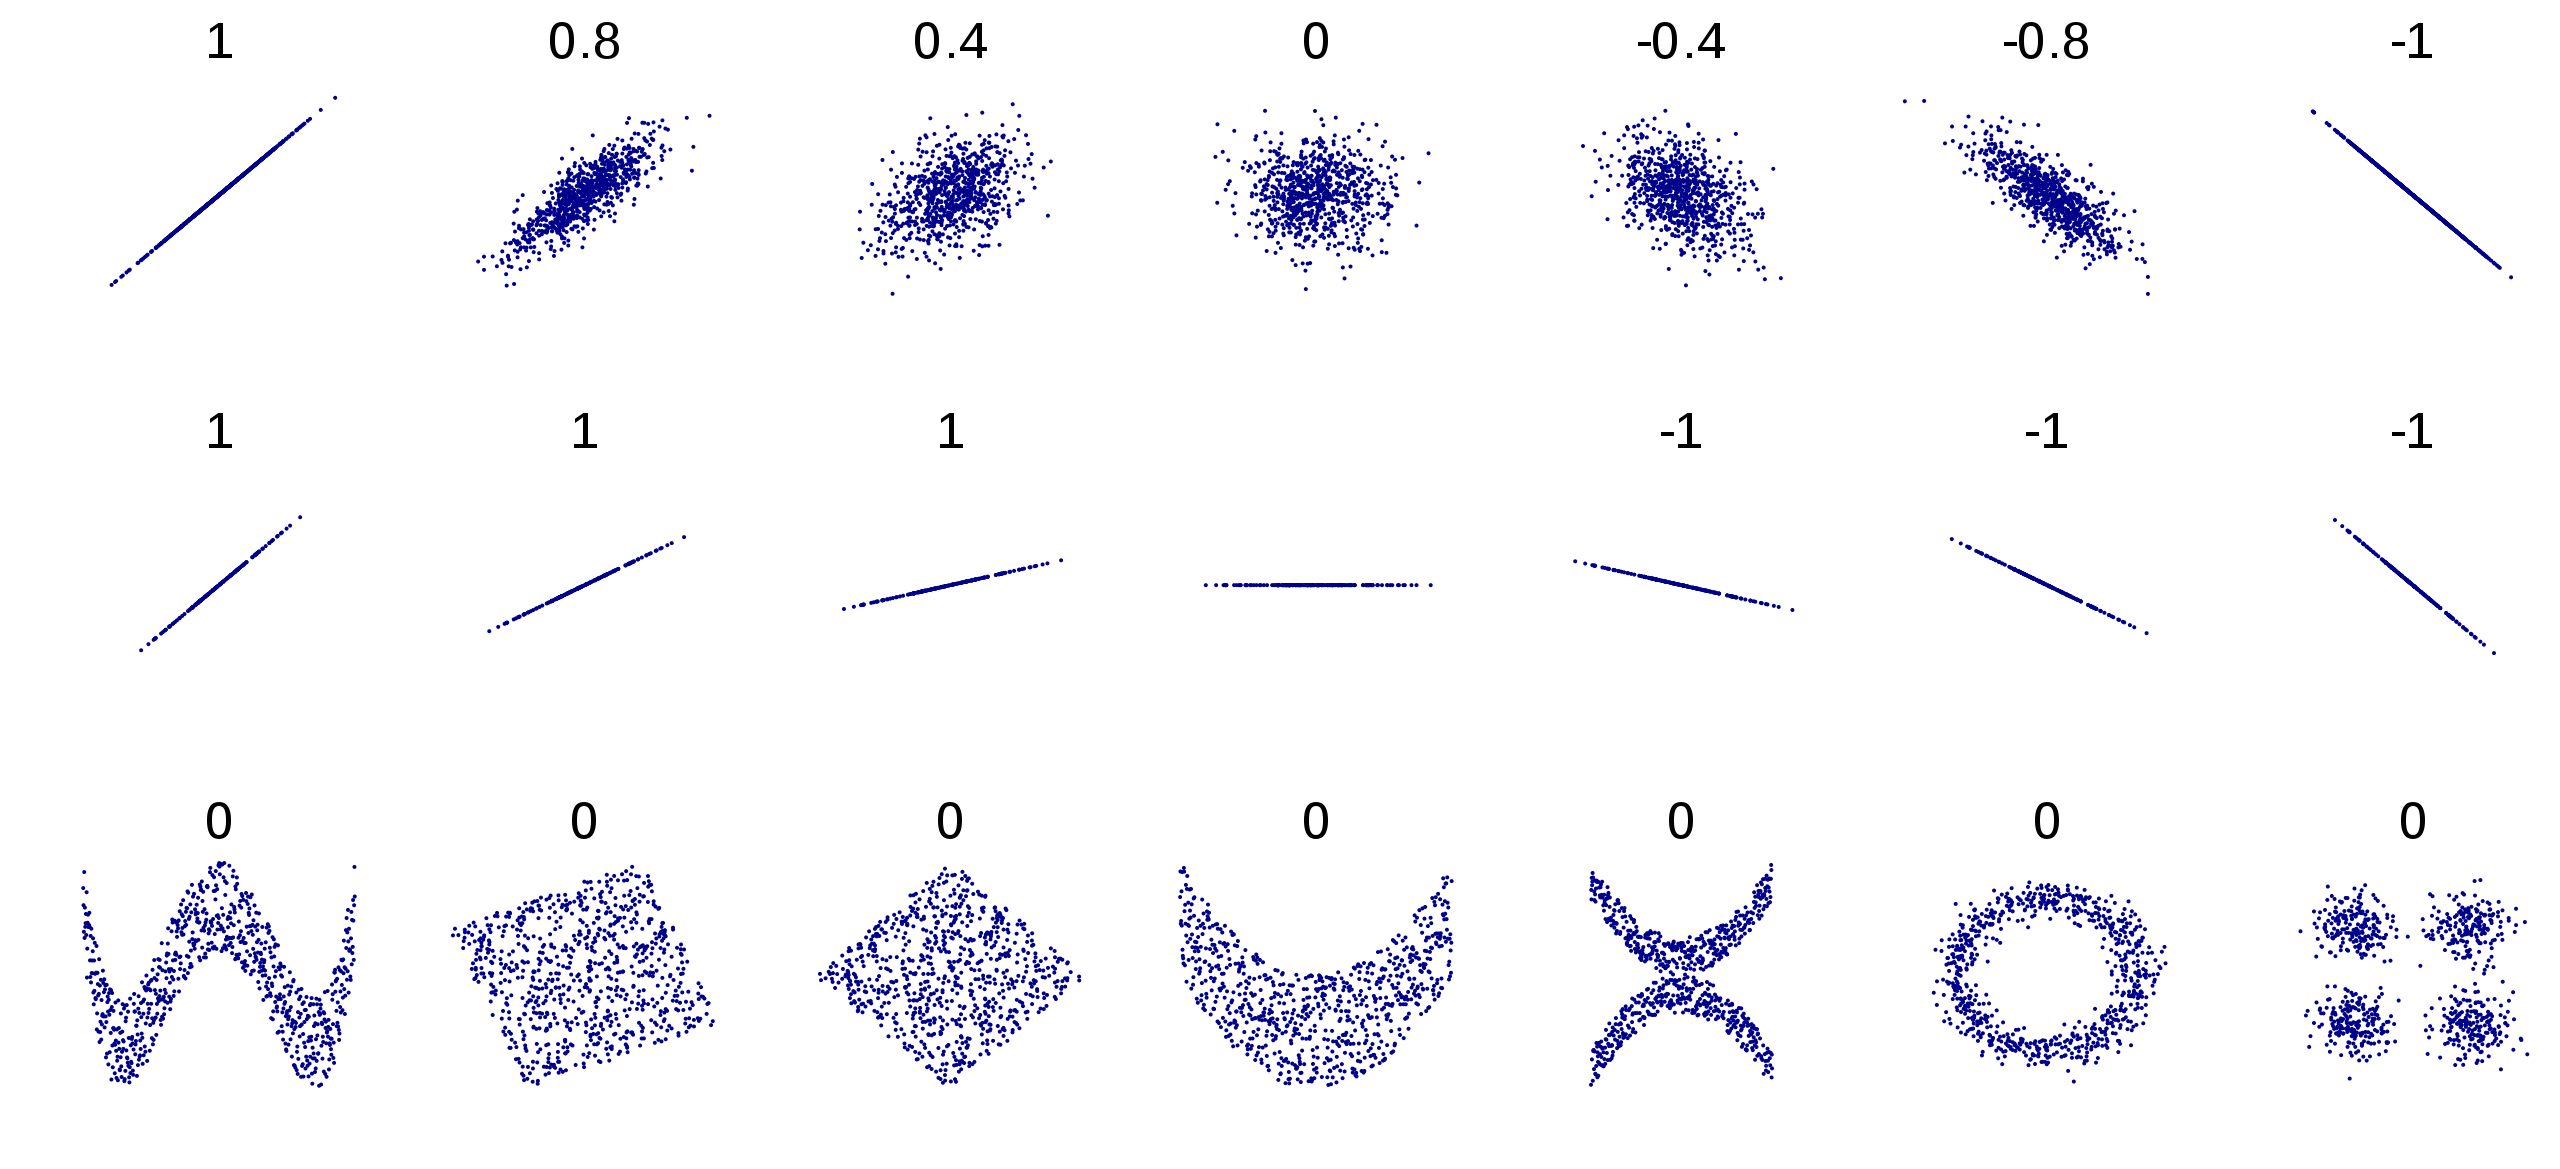
\includegraphics[scale=0.137]{img/corr}
\caption{Plots of correlated and non correlated variables.}
\label{corr}
\end{figure}
\subsection{Gaussian functions and Gaussian distributions}
\index{Gaussian functions}
\index{Gaussian distributions}
\label{gaussian}
\begin{definition}{\textbf{Gaussian function}}
A Gaussian function is a mathematical function in the form:
\begin{equation}
f(x) = a e^{-\frac{(x-b)^2}{2c^2}}
\end{equation}
The Gaussian function has three parameters $a$,$b$ and $c$. The graph of a Gaussian function is the Bell curve. The parameter $a$ is the height of the curve's peak, $b$ is the position of the peak and $c$ the \textit{standard deviation} controls the width of the bell.

An important property of the Gaussian function is that the product of two Gaussian functions is still a Gaussian function:
\begin{equation}
\label{gauss2}
\begin{aligned}
&f(x) \cdot g(x) = a e^{-\frac{(x-b)^2}{2c^2}} a_1 e^{-\frac{(x-b_1)^2}{2c_1^2}} = (a\cdot a_1) e^{-\frac{x^2-2bx+b^2 + x^2-2b_1x+b_1^2}{2c^2 2c_1^2}}=\\
&= (a\cdot a_1) e^{-\frac{2x^2-2x(b+b_1)+ b^2 +b_1^2}{2c^2 2c_1^2}} = (a\cdot a_1) e^{-\frac{x^2-2x\frac{b +b_1}{2}+ \frac{b^2 +b_1^2}{2}}{2c^2 c_1^2}} = \\
&=(a\cdot a_1) e^{-\frac{x^2-2x\frac{b +b_1}{2}+ \frac{b^2 +b_1^2}{2}}{2c^2 c_1^2}} e^{\frac{\br{\frac{b +b_1}{2}}^2 - \br{\frac{b+b_1}{2}}^2 } {2c^2 c_1^2}}=  \\
&=(a\cdot a_1) e^{-\frac{x^2-2x\frac{b +b_1}{2}+\br{\frac{b +b_1}{2}}^2}{2c^2 c_1^2}} e^{\frac{\br{\frac{b +b_1}{2}}^2 - \frac{b^2 +b_1^2}{2}} {2c^2 c_1^2}} = \\
&=(a\cdot a_1) e^{-\frac{\br{x-\frac{b +b_1}{2}}^2}{2c^2 c_1^2}} e^{\frac{\br{\frac{b +b_1}{2}}^2 - \frac{b^2 +b_1^2}{2}} {2c^2 c_1^2}} = \\
&= a_2 e^{-\frac{\br{x-\frac{b +b_1}{2}}^2}{2c^2 c_1^2}} = a_2 e^{-\frac{\br{x-b_2}^2}{2c_2^2}}
\end{aligned}
\end{equation}
\end{definition}

\begin{definition}{\textbf{Gaussian distribution}}
A normalized Guassian function or normal distribution is a Gaussian function with an area under the curve equal to $1$. Hence it can be interpreted as a probability distribution.

To find the formula let us force the curve to have area $1$:

\begin{equation}
\int_{-\infty}^{\infty} a e^{-\frac{(y-b)^2}{2c^2}} dy = a \int_{-\infty}^{\infty} e^{-\frac{(y-b)^2}{2c^2}} dy
\end{equation}
and performing a change of integration variable:
\begin{equation}
\begin{aligned}
&\frac{y-b}{\sqrt{2}c} = x \Rightarrow dx = dy \frac{1}{\sqrt{2}c} dx \Rightarrow dy = \sqrt{2}c dx\\
&a \int_{-\infty}^{\infty} e^{-\frac{(y-b)^2}{2c^2}} dy = \sqrt{2}ac  \int_{-\infty}^{\infty} e^{-x^2} dx 
\end{aligned}
\end{equation}
where  $ \sqrt{2}c$ is a constant so that in can be moved out of the integral. From now on we will focus just on the integral.

Unfortunately the integral has not solutions with elementary functions (Louiville theorem, see Abstract Algebra). However the definite integral exists (demonstration is skipped) and it is:
\begin{equation}
\int_{-\infty}^{\infty} e^{-x^2} dx = \sqrt{\pi}
\end{equation}

To have area equal to $1$ we must have:
\begin{equation}
ac\sqrt{2\pi} = 1 \Rightarrow a =  \frac{1}{\sqrt{2\pi}c}
\end{equation}
So now the function is defined by just 2 parameters. 

Normally $b=\mu$ and is the mean of the function while $c=\sigma$ is the standard deviation.

As opposed to the Gaussian function, multiplying two of these functions we do not get another gaussian distribution, but a scaled guassian distribution. If the Gaussian functions have 0-mean and $\sigma^2=1$ then the product is still Guassian distribution with $0$-mean and $\sigma^2=1$.
\end{definition}

\begin{definition}{\textbf{Standard Normal Gaussian distribution}}
A Standard Normal Gaussian distribution is a Gaussian distribution with $0$ mean and standard deviation $1$.
\end{definition}


\subsection{Hermitian function}
\begin{definition}{\tb{Hermitian function}}
\label{Hermitian}
An hermitian function is a complex function for which its complex conjugate is equal to the original function with the variable changed of sign:
\begin{equation}
\bar{f(x)} = f(-x)
\end{equation}
where the bar indicates the complex conjugate.
From this definition it follows immediately that $f$ is a Hermitian function if and only if:
\begin{itemize}
\item the real part of $f$ is an even function;
\item the imaginary part of $f$ is an odd function.
\end{itemize}
\end{definition}

\subsection{Non-negative definite kernels}
\begin{definition}{\tb{Non-negative definite kernels}}
$K$ is said to be non-negative definite (or positive semidefinite) iff
\begin{equation}
\sum _{i=1}^{n}\sum _{j=1}^{n}K(x_{i},x_{j})c_{i}c_{j}\geq 0
\end{equation}
for all finite sequences of points $\forall x_i,x_j \in \CMcal{X}$ and $\forall c_i, c_j \in \CMcal{R}$.
\end{definition}

%%%%%%%%%%%%%%%%%%%%%%%%%%%%%%%%%%%%%%%%%%%%%%%%%%%%%%%%%%
%%%%%%%%------------------------------NEW SECTION------------------------------%%%%%%%%%
%%%%%%%%%%%%%%%%%%%%%%%%%%%%%%%%%%%%%%%%%%%%%%%%%%%%%%%%%%
\newpage
\section{Useful mathematical tricks}
\subsection{First and second order Taylor approximation for multi variable scalar functions}
\label{subsec:Taylor}
It is known from analysis that a single variable  infinitely differentiable function in some open interval around $x=a$, can be expressed around that point, with the Taylor series:
\begin{equation}
f(x) = \displaystyle \sum_{k=0}^\infty \frac{\left. f^{(k)}\right|_{x=a} }{k!} (x-a)^k
\end{equation}

Now we want to generalize the formula for scalar-valued functions of multiple variables\footnote{\url{https://mathinsight.org/taylors_theorem_multivariable_introduction}}:
\begin{equation}
f(\x) = f(x_1, x_2, \cdots,x_n)
\end{equation}
Given a point $a$, for a multi variable differentiable function $f(x,y)$, its first order approximation is given by
\begin{equation}
f(\x) \approx f(a) + Df(\mathbf{a}) + (\x -\mathbf{a})
\end{equation}
where $Df(\mathbf{a})$ is the matrix of partial derivatives. The first order approximation the hyper-plane tangent to the curve in $a$, as well as the first-order Taylor polynomial.

For the second quadratic approximation one has to add quadratic terms to the linear approximation, i.e., the analogous of second derivative in a hyper-space. Since $f(x)$ is scalar, the first derivative is $Df(x)$, a $1\times n$ matrix, which we can view as an $n$-dimensional vector-valued function of the $n$-dimensional vector $\x$. For the second derivative of $f(x)$, we can take the matrix of partial derivatives of the function $Df(x)$. We could write it as $DDf(x)$ for the moment. This second derivative matrix is an $n\times n$ matrix called the Hessian matrix of $f$. We'll denote it by $Hf(x)$:
\begin{equation}
Hf(\x) =\begin{pmatrix}
\frac{\partial^2 f}{\partial x_1^2}\ \frac{\partial^2 f}{ \partial x_1 \partial x_2} & \cdots & \frac{\partial^2 f}{\partial x_1 \partial x_n}\\
\frac{\partial^2 f}{\partial x_2} \partial x_1\ \frac{\partial^2 f}{ \partial x_2^2} & \cdots & \frac{\partial^2 f}{\partial x_2 \partial x_n}\\
\vdots&\vdots&\vdots&\vdots\\
\frac{\partial^2 f}{\partial x_n \partial x_1}\ \frac{\partial^2 f}{ \partial x_n \partial x_2} & \cdots & \frac{\partial^2 f}{\partial x_n^2}\\
\end{pmatrix}
\end{equation}
or equivalently $Hf(\x) = DDf(\x)$. When $f$ is a function of multiple variables, the second derivative term in the Taylor series will use the Hessian $Hf(\mathbf{a})$. For one dimension we have $\frac{1}{2}(x-a)f^{''}(a)(x-a)$. The analogue of this expression is: $\frac{1}{2}(\x-\mathbf{a})Hf(\mathbf{a})(\mathbf{a})(\x-\mathbf{a})$

So the second order approximation is:
\begin{equation}
f(\x) \approx f(a) + Df(\mathbf{a}) + (\x -\mathbf{a}) + \frac{1}{2}(\x-\mathbf{a})Hf(\mathbf{a})(\x-\mathbf{a})
\end{equation}

\subsection{Cauchy-Schwarz inequality}
\label{sec:CauchySchwarz}
The Cauchy-Schwarz inequality states that for all vectors $u$ and $v$ of an inner product space, it is true that:
\begin{equation}
\left| \langle \mathbf{u}, \mathbf{v} \rangle \right|^2 \le \langle \mathbf{u}, \mathbf{u} \rangle\cdot \langle \mathbf{v}, \mathbf{v} \rangle = \| \mathbf{u}\| \cdot \| \mathbf{v}\|
\end{equation}
with equality holding only when the two vectors are linear dependent, i.e., they are parallel.

\subsection{Sum of decreasing numbers}
\label{sec:SumDecreasingNumber}
Consider a number $n$ and assume one wants to compute its decreasing number:
\begin{equation}
S = n + n-1 +\cdots 1
\end{equation}
The sum is equal to
\begin{equation}
S = \frac{n\cdot (n+1)}{2}
\end{equation}
\begin{proof}
We express the sum in both ways:
\begin{equation}
\begin{aligned}
S = n + &n-1 +\cdots 1\\
S = 1 + &2 +\cdots n\\
\end{aligned}
\end{equation}
Summing term by term, i.e., the first term with the first, the second with the second and so on:
\begin{equation}
2S = (n+1) + (n+1) + \cdots + (n+1) = (n+1) \cdot n \Rightarrow S = \frac{(n+1) \cdot n}{2}
\end{equation}
\end{proof}

\subsection{The Heaviside cover-up method}
\label{coverupMethod}
The cover-up method can be used to make a partial fractions decomposition of a rational function $\frac{p(x)}{q(x)}$ whenever the denominator can be factored into distinct linear factors. Suppose we want to decompose: $\frac{x-7}{(x-1)(x+2)}$, we know the decomposition will have the form:
\begin{equation*}
\frac{x-7}{(x-1)(x+2)} = \frac{A}{x-1} +\frac{B}{x+2}
\end{equation*}
To determine $A$ by the cover-up method, on the left-hand side we mentally remove (or cover up with a finger) the factor $x-1$ associated with $A$, and substitute $x=1$ into what's left; this gives $A$:
\begin{equation*}
\frac{x-7}{\quad\quad(x+2)}\bigg\rvert_{x=1} = -2 = A
\end{equation*}
Similarly for $B$:
\begin{equation*}
\frac{x-7}{(x+1)\quad\quad}\bigg\rvert_{x=-2} = 3 = B
\end{equation*}

The method of using the partial fraction decomposition is successful ONLY for proper rational functions. In what follows, we will assume that we are dealing with such a proper function.
If the degree of P is larger than or equal to the degree of $q$, apply long division to reduce the problem to that of integrating the sum of a polynomial and a proper rational function \footnote{\url{http://www.math.udel.edu/~angell/partfrac.pdf}}. Given two polynomials $p(x)$ and $q(x)$ and their ratio $\frac{p(x)}{q(x)}$, we divide the method into four cases, depending on the nature of the real factors of $q$.
\paragraph{\tb{Case $1$: the denominator $q$ can be factored into linear factors all different.}}

\begin{proof}
In general, if the denominator of the rational function factors into the product of distinct linear factors:
\begin{equation}
\frac{p(x)}{(x-a_1) (x-a_2)\cdots (x-a_n)} = \frac{A_1}{x-a_1} + \frac{A_2}{x-a_2} + \cdots+ \frac{A_n}{x-a_n} 
\end{equation}
with $a_i \ne a_j$ for $i\ne j$.
Now to find $A_i$ we multiply both members by $x-a_i$ and take the limit for $x\rightarrow a_i$:
\begin{equation}
\begin{aligned}
\lim_{x\rightarrow a_i}\frac{p(x)}{(x-a_2)\cdots(x-a_n)} &= \\
&= \lim_{x\rightarrow a_i} \left[A_1 + \cancel{(x-a_1) \br{\frac{A_2}{x-a_2} + \cdots+ \frac{A_n}{x-a_n} }}\right]
\end{aligned}
\end{equation}
Now the right member will consist just of $A_1$ since all the other terms are multiplied by a quantity that goes to $0$. Then we can find $A_1$  by substituting $x=a_1$:
\begin{equation}
A_1 = \frac{p(a_1)}{(a_1-a_2)\cdots(a_1-a_n)}
\end{equation}
\end{proof}

\paragraph{\tb{Case $2$}: the polynomial $q$ can be factored into linear factors, some of which are repeated}
The cover-up method can also be used if a linear factor is repeated, but there too it gives just partial results. It applies only to the highest power of the linear factor. For example:
\begin{equation}
\begin{aligned}
\frac{1}{(x-1)^2(x+2)} = \frac{A}{(x-1)^2}  +\frac{B}{(x-1)}  +\frac{C}{(x+2)}
\end{aligned}
\end{equation}
To find up $A$, cover up $(x-1)^2$ and set $x=1$: $A=\frac{1}{3}$.  To find up $C$, cover up $(x+2)$ and set $x=-2$: $C=\frac{1}{9}$. This leaves $B$ which cannot be found by the cover-up method. But since $A$ and $C$ are already known, $B$ can be found by substituting any numerical value (other than $1$ or $-2$) for $x$ in the equation. For example $x=0 \Rightarrow B=\frac{-1}{9}$.

\paragraph{\tb{Case $3$:} the polynomial Q can be factored into linear and quadratic factors, and none of the quadratic factors is repeated}. In this case, each unrepeated quadratic factor gives rise to a term of the form
\begin{equation}
\frac{3x^2+x-2}{(x^2+1)(x-1)} = \frac{A_1}{(x-1)}+\frac{A_2}{(x^2+1)}
\end{equation}

\paragraph{\tb{Case 4}}The polynomial $q$ can be factored into linear and quadratic factors, and some of the quadratic factors are repeated.
\begin{equation}
\frac{2x^3 + 3x^2+x-1}{(x^2+2x+1)^2(x+1)} = \frac{A_1}{(x+1)}+\frac{A_2x +A_3}{((x^2+2x+1)}+\frac{A_4x +A_5}{((x^2+2x+1)^2}
\end{equation}


Heaviside's cover-up method also can be used even when the denominator doesn't factor into distinct linear factors. To be sure, it gives only partial results, but these can often be a big help. We illustrate.
\begin{equation*}
\frac{5x+6}{(x^2+4)(x-2)} = \frac{Ax+B}{(x^2+4)} +\frac{C}{(x-2)} 
\end{equation*}
We first determine $C$ by the cover-up method, getting $C = 2$ . Then $A$ and $B$ can be found by the method of undetermined coefficients; the work is greatly reduced since we need to solve only two simultaneous equations to find $A$ and $B$, not three:
\begin{equation}
5x + 6 = (Ax + B)(x - 2) + 2(x^2 + 4)\Rightarrow A=-2, \quad B=1
\end{equation}




%%%%%%%%%%%%%%%%%%%%%%%%%%%%%%%%%%%%%%%%%%%%%%%%%%%%%%%%%%
%%%%%%%%------------------------------NEW SECTION------------------------------%%%%%%%%%
%%%%%%%%%%%%%%%%%%%%%%%%%%%%%%%%%%%%%%%%%%%%%%%%%%%%%%%%%%
\newpage
\section{Statistical Decision Theory}
\subsection{Expected prediction error}
Let $X \in \R^p$ denote a real valued random input vector, and $Y \in \R^p$ a real valued random output variable, with joint distribution $Pr(X,Y)$. We seek a function $f(X)$ for predicting $Y$ given values of the input $X$. This theory requires a loss function $L(Y,f(X))$ for penalizing errors in prediction, and by far the most common and convenient is 
squared error loss: $L(Y,f(X))=(Y -f(X))^2$.

The estimated prediction error is 

\begin{equation}
\begin{aligned}
EPE(f) &= \E\left[ \left( Y- f(X) \right)^2 \right] = \int \left( y- f(x) \right)^2 p(x,y) dx dy \\
&= \int_x\int_y \left( y- f(x) \right)^2 p(x,y) dx dy \\
\end{aligned}
\end{equation}

Recalling $p(x,y) = p( y|x) p(x)$:
\begin{equation}
\begin{aligned}
EPE(f) &= \int_x\int_y \left( y- f(x) \right)^2 p(y|x)  p(x) dx dy \\
 &= \int_x \int_y \left( \left( y - f(x) \right)^2 p(y|x) dy\right)  p(x) dx   \\
 &= \int_x \E_{Y|X} \left[ \left( y - f(X) \right)^2 | X=x \right]  p(x) dx   \\
 &= \E_X \left[ \E_{Y|X} \left[ \left( y - f(X) \right)^2 | X=x \right]    \right]   
\end{aligned}
\end{equation}
So to minimize the prediction error:
\begin{align}
f(x) &= \argmin{c} \E_{Y|X} \left[ \left( y - c(x) \right)^2 | X=x \right] 
& \Rightarrow f(x) = \E \left[ Y | X=x \right] 
\end{align}

The \textit{Nearest Neighbour} algorithm, assigns labels to points by counting and averaging the labels of the points belonging to a given neighbourhood:

\begin{align}
\hat{f} (x) &= Ave \left(   y_i|x_i \in N_k(x)   \right)
\end{align}
where $N_k(x) $ contains the $k$ points closest to $x$. This presents \textbf{two approximations}
\begin{itemize}
\item expectation is approximated by averaging
\item conditioning at a point is relaxed to conditioning on some region centred at the target point.
\end{itemize}

With $k$ sufficiently large, the average gets more stable and with large $N$ the points will be more likely close to x. If $k, N \rightarrow \infty$ with $k/N \rightarrow 0$ the average becomes the expectation and we have the best possible estimator.

Unfortunately often we do not have so much data and some other times we might want exploit the supposed structure of data (linear, polynomial etc.).

However there is even a bigger problem when there are too many dimensions (i.e., $p$ is large). Consider a uniformly distributed input in a $p$ dimensional unit hypercube. Consider a hypercube neighbourhood around the target point capturing a fraction $r$ of the total observations distributed among the unit hypercube. The edge of the neighbour hypercube will be $e_p(r) = r^{1/p}$. In 10 dimensions, using a neighborhood capturing $1\%$ of the data we have $r(0.01) = 0.63$ so we must use 63\% of the total data for one target.

On the contrary the linear regression is a \textbf{model-based approach}, i.e., one assumes that the function $f(x)$ is approximately linear:
\begin{align}
f(x) &\approx x^T \beta
\end{align}

Putting this in the $EPE$ equation:

\begin{equation}
\begin{aligned}
f(x) &= \argmin{c} \E_{Y|X} \left[ \left( y - c(x) \right)^2 | X=x \right]  \\
&= \argmin{\beta} \E_{Y|X} \left[ \left( y - x^T \beta \right)^2 | X=x \right] \\
\Rightarrow \beta &= \left[ \E\left[ X\cdot X ^T\right]\right]^{-1} \cdot \E\left[ X\cdot Y \right]
\end{aligned}
\end{equation}

The minimum of a quadratic function is given by deriving and setting its derivative to $0$.

If instead of a $L_2$ loss function we use $L_1$

\begin{equation}
\begin{aligned}
EPE(f) &= \E\left[ \left| Y- f(X) \right| \right] = \int \left| y- f(x) \right| p(x,y) dx dy \\
&= \int_x\int_y \left| y- f(x) \right|p(x,y) dx dy \\
\end{aligned}
\end{equation}
Recalling $p(x,y) = p( y|x) p(x)$:
\begin{equation}
\begin{aligned}
EPE(f) &= \int_x\int_y \left| y- f(x) \right|p(y|x)  p(x) dx dy \\
 &= \int_x \int_y \left| \left( y - f(x) \right| p(y|x) dy\right)  p(x) dx   \\
 &= \int_x \E_{Y|X} \left[ \left| y - f(X) \right| | X=x \right]  p(x) dx   \\
 &= \E_X \left[ \E_{Y|X} \left[ \left| y - f(X) \right| | X=x \right]    \right]   
\end{aligned}
\end{equation}

\begin{equation}
\begin{aligned}
f(x) &= \argmin{c} \E_{Y|X} \left[ \left| y - c(x) \right| | X=x \right]
\end{aligned}
\end{equation}
and as already seen in \autoref{medianMin}, the minimizer for the sum of distances is the median.
\subsubsection{Loss function for categorical variables}
For categorical output variables $\mathbb{G}_k$ we have: 

\begin{equation}
\begin{aligned}
EPE = \E\left[ L\left( G, \hat{G}(X)\right)\right] = \E_x \sum_{k=1}^K L\left[ \mathbb{G}_k, \hat{G}(X)\right]Pr\left( \mathbb{G}_k|X\right)
\end{aligned}
\end{equation}
where the expectation is again taken with respect to the joint distribution $Pr(G,X)$. Conditioning again we can write:
\begin{equation}
\begin{aligned}
EPE = \E_x \sum_{k=1}^K L\left[ \mathbb{G}_k, \hat{G}(X)\right]Pr\left( \mathbb{G}_k|X\right)
\end{aligned}
\end{equation}
where the integral over $y$ has been substituted with the summation due to the categorical nature of the variable.

The minimizer is given by:

\begin{equation}
\begin{aligned}
\hat{G}(x) = \argmin{g \in \mathbb{G}} \sum_{k=1}^{K} L\left( \mathbb{G}_k, g\right)Pr\left( \mathbb{G}_k | X=x \right)
\end{aligned}
\end{equation}

Often the \textit{zero-one loss function} is used for categorical variables and the above simplifies to:
\begin{equation}
\begin{aligned}
\hat{G}(x) = \argmin{g \in \mathbb{G}}  \left[1 - Pr\left( g | X=x \right) \right] =\argmax{g \in \mathbb{G}}  \left[Pr\left( g | X=x \right) \right]
\end{aligned}
\end{equation}
This is known as \textit{Bayes classifier} because \textbf{it classifies to the most probable class, using conditional discrete probability distribution}.

\paragraph{\textbf{Note}: When models or loss functions use additional parameters that penalize complexity (Lasso, Ridge and others) we cannot use the training data to determine these parameters, since we would pick those that gave interpolating fits with zero residuals but it will be unlikely to predict future data.}

\subsection{Bias-Variance trade-off}
\begin{equation}
\begin{aligned}
EPE(f) &= \E \left[ \left( Y- f(X) \right)^2 \right] =\\
            &= \E \left[ Y^2\right] - 2 \E \left[ Y\right] \E\left[ f(X)\right] + \E\left[ f(X)^2\right]\\
             &= Y^2 - 2  Y \E\left[ f(X)\right] + \E\left[ f(X)^2\right]
\end{aligned}
\end{equation}

Recalling 
\begin{equation}
\begin{aligned}
&BIAS\left(Y,\E\left[f(X)\right]\right) = \left| Y-\E\left[f(X)\right]\right| \\
&\Rightarrow BIAS\left(Y,f(X)\right)^2 = \left( Y-\E\left[f(X)\right]\right)^2 \\
&= Y^2 -2 Y \E\left[f(X)\right] + \E\left[f(X)\right]^2 \\
\end{aligned}
\end{equation}

$EPE$ can be expressed using also the Variance definition in \autoref{Variance}
\begin{equation}
\begin{aligned}
\label{biasVar}
EPE(f) &=  Y^2 - 2  Y \E\left[ f(X)\right] + \E\left[ f(X)^2\right] +\E\left[f(X)\right]^2-\E\left[f(X)\right]^2\\
&= BIAS(Y, f(X)^2 + \Var(Y, f(x))
\end{aligned}
\end{equation}

The bias is given by the distance of our predictions from real points. Complex models have more degrees of freedom and are able to fit closer real points hence they to tend to have low bias. However, they present higher variance. On the contrary simple models (i.e., linear) have lower variance but higher bias.

The error due to variance is the amount by which the prediction, over one training set, differs from the expected predicted value, over all the training sets. As with bias, you can repeat the entire model building process multiple times. To paraphrase Manning et al (2008), variance measures how inconsistent are the predictions from one another, over different training sets, not whether they are accurate or not.  A learning algorithm with low bias must be "flexible" so that it can fit the data well. But if the learning algorithm is too flexible, it will fit each training data set differently, and hence have high variance.

For linear models fit by ordinary least squares, the estimation bias is zero. For restricted fits, such as ridge regression, it is positive, and we trade it off with the benefits of a reduced variance.

%%%%%%%%%%%%%%%%%%%%%%%%%%%%%%%%%%%%%%%%%%%%%%%%%%%%%%%%%%
%%%%%%%%------------------------------NEW SECTION------------------------------%%%%%%%%%
%%%%%%%%%%%%%%%%%%%%%%%%%%%%%%%%%%%%%%%%%%%%%%%%%%%%%%%%%%
\newpage
\section{Taxonomy of machine learning algorithms}
\subsection{Supervised vs Unsupervised}
The first distinction is between Supervised and Unsupervised learning. Some in-between methods exist too:
\begin{itemize}
\item \textbf{supervised learning}: the training data you feed to the algorithm includes the desired solutions, called labels. Typical algorithms are Linear regression, K-Nearest Neighbours, Logistic Regression,  Support Vector Machines, Decision Trees and Random Forests, Neural Networks. Tasks of supervised learning are \textbf{classification} and \textbf{prediction}, i.e., \textbf{regression}.
\item \textbf{unsupervised learning}: no label is passed as input and typical the algorithm must apply label or group data somehow. Its tasks are 
\begin{itemize}
\item \textbf{clustering}: whose goals is to group together similar groups. This is typically done by defining a measure of similarity (or dissimilarity) between points in the hyperspace. Popular algorithms are K-means, Hierarchical clustering Analysis, Expectation Maximization; 
\item \textbf{Visualization and dimensionality reduction}: for visualization applications, one feeds them a lot of complex and unlabeled data, and they output a 2D or 3D representation of your data that can easily be plotted. The goal of dimensionality reduction instead is to simplify the data without losing too much information by merging correlated features. Popular algorithms are Principal component analysis (PCA), Kernel PCA, Locally-Linear Embedding, t-distributed Stochastic Neighbour Embedding
\item \textbf{Association Rule Learning}: Apriori, Eclat.
\end{itemize}
\item \textbf{semi-supervised learning}: Some algorithms can deal with partially labeled training data, usually a lot of unlabeled data and a little bit of labeled data. Some photo-hosting services, such as Google Photos, are good examples of this. Once you upload all your family photos to the service, it automatically recognizes that the same person.
\item \textbf{Reinforcement learning}: The learning system, called an agent in this context, can observe the environment, select and perform actions, and get rewards or penalties in return. It must then learn by itself what is the best strategy, called a \textbf{policy}, to get the most reward over time.
\end{itemize}

\subsection{Batch and online Learning}
Another criterion used to classify Machine Learning systems is whether or not the system can learn incrementally from a stream of incoming data.
\begin{itemize}
\item \textbf{batch-learning}: the system is incapable of learning incrementally: it must be trained using all the available data. this is called \textbf{offline learning}.
\item \textbf{online learning}: you train the system incrementally by feeding it data instances sequentially, either individually or by small groups called mini-batches. Online learning is great for systems that receive data as a continuous flow (e.g., stock prices) and need to adapt to change rapidly or autonomously. It is also a good option if you have limited computing resources.
\end{itemize}

\subsection{Instance-based vs Model based}
\begin{itemize}
\item \textbf{instance-based learning}: the system learns the examples by heart, for example by using a measure of similarity such as number of similar words in two emails to classify spam emails.
\item \textbf{Model-based learning}: it builds a model to perform predictions
\end{itemize}

%%%%%%%%%%%%%%%%%%%%%%%%%%%%%%%%%%%%%%%%%%%%%%%%%%%%%%%%%%
%%%%%%%%------------------------------NEW SECTION------------------------------%%%%%%%%%
%%%%%%%%%%%%%%%%%%%%%%%%%%%%%%%%%%%%%%%%%%%%%%%%%%%%%%%%%%
\newpage
\section{Hands on datasets}
Before looking at the machine learning algorithms, let us focus on how to prepare data to be fed to the algorithms. The focus is on the \textit{scikit-learn} and \textit{Pandas} libraries in Python and .

\subsection{Looking at data}
After having loaded the data in a Pandas dataframe, there are methods of this data structure that allow to get some information from the data:
\begin{itemize}
\item \textbf{\textit{df.head()}}: this method allows to get a gist on the general structure of the dataframe by looking at the value of the first 5 rows. More rows can be shown by passing as input the desired number to be shown;

\item \textbf{\textit{df.info()}}: it tells the number of entries and for each column its type and the number of non-null elements. Note that string type is considered in a more general type as \textit{object} type;
\item \textbf{\textit{df['field'].value\_counts()}}: this is useful when \textit{field} is a categorical. It shows all the possible values in the dataframe for the column and for each one the number of entries having that column value;
\item \textbf{\textit{df.describe()}}: this method performs some statistics on numerical attributes (null values are ignored). Particularly, it calculates the number of entries (with valid values), the mean, standard deviation, minimum and maximum and the $25\%, 50\%, 75\%$ percentiles.
\item\textbf{\textit{df.hist(bins=20)}}: it plots the histogram of each numerical value. The number of bins tells how many bars (i.e., how many groups) the histogram should have;
\item\textbf{\textit{df.corr()['attribute'].sort\_values(ascending=False)}}: shows the correlation between the selected attribute and all the others. Remember that the correlation an indication of linear relationships only;
\item\textbf{\textit{scatter\_matrix(h[attributes], figsize=(12,8))}}: plots every numerical attribute against every other numerical attribute (carefulness is needed when the number of attribute is large). To give some sense to the main-diagonal plots, a histogram is plotted by the function itself. See \autoref{scatterplot}.
\end{itemize}

Some inferences can be made from the histogram. First of all the units and scales; there even might be some hints if values have been cupped (for example when there is a natural decreasing trend but the last bin has a value significantly bigger than the others).

\subsection{Train and test set}
The first thing to do is to split the set between train and test. A good idea is to have the same split across different runs of the algorithms. One solution is to save the data-set and load it next times. Another solution is to use random generator seeds so that the pseudo-random sequence starts every-time from the same point. But these solutions will break next time one fetches an updated dataset. 

A common solution is to use each instance's identifier to decide whether or not it should go in the test set (assuming instances have a unique and immutable identifier). For example, you could compute a hash of each instance's identifier, keep only the last byte of the hash, and put the instance in the test set if this value is lower or equal to 51 (~20\% of 256). This ensures that the test set will remain consistent across multiple runs, even if you refresh the dataset. It is assuming a uniform distribution by hash algorithm. This can be implemented with the following functions:

\begin{lstlisting}[caption=Example of function to split according to the last by of the hash on the id.]
def split_train_test_by_id(data, test_ratio, id_column, 
		                        hash=hashlib.md5):
    ids = data[id_column];
    in_test_set = ids.apply(lambda _id: test_set_check(_id,  test_ratio, hash));
    return data.loc[~in_test_set], data.loc[in_test_set];

# The check on the id is to see the value of the last byte
# If this value is less then test_ratio*256 (assuming uniform 
# distribution) 
# then will return true otherwise false. The fraction of true
# will be  equal to test_ratio
def test_set_check(identifier, test_ratio, hash):
    limit = test_ratio*256; #1byte
     #digest will calculate the hash value 
    res = hash(np.int64(identifier)).digest()[-1];
    return res<limit;
\end{lstlisting}

However, there is a \tb{further problem} if there is not an identifier column. The solution is to create one. It is possible to use the row index but the one has make sure new data are appended in order and no data should not be deleted.If this is not possible, then you can try to use the most stable features to build a unique identifier. For example, a district's latitude and longitude are guaranteed to be stable for a few million years, so one could combine them into an ID like so and their values are unique:
\begin{lstlisting}[caption="Creating a column ID from stable features such as latitude and longitude.]
df["id"] = df['longitude']*1000+df['latitude']
\end{lstlisting}

\subsubsection{Stratified sampling}
Consider a given value, either categorical or numerical. Generally, they are not uniformly distributed among the entries. As the simplest possible example consider that in a data set of people women are the $60\%$, and men $40\%$. When splitting between train and test set it is better to keep this ratio, especially when some values are rarer.

This is true also for numerical value: in this case, one first needs to create a corresponding categorical attribute. It is important to have sufficient data for each category and at the same time categories must be representatives. First a range size is chosen (the range of the new categorical value) and it is used to divide the original values. Then the resulting valued are ceiled. Clapping is required.

After that, it is possible to stratify-sampling. \ti{scikit-learn} has the function \ti{StratifiedShuffleSplit} to perform it:
\begin{lstlisting}
from sklearn.model_selection import StratifiedShuffleSplit
split = StratifiedShuffleSplit(n_splits=1, test_size=0.2, random_state=42);
\end{lstlisting}

\subsection{Plotting the dataset}
Visualing data can give other insights.
Pandas dataframe has a plot method:
\begin{lstlisting}[caption=Example of Pandas dataframe plot method.]
df.plot(kind="scatter", x="longitude", y="latitude", alpha=0.2);
\end{lstlisting}
In this way one gets darker areas according to the number of elements.
It is also to make more complex graphs: for example we can use colormaps to represent the intensity of output and circle radius to represent another feature of the data:
\begin{lstlisting}[caption=Example of Pandas dataframe plot with colormap and variable radius of scattered circles.]
h.plot(kind="scatter",x="longitude", y="latitude", alpha=0.4, 
		s = h['population']/100,  label="popultion", 
		c="median_house_value", cmap = plt.get_cmap('jet'), 
		colorbar=True, figsize=(15,8));
plt.legend();
\end{lstlisting}

\begin{figure}
\centering
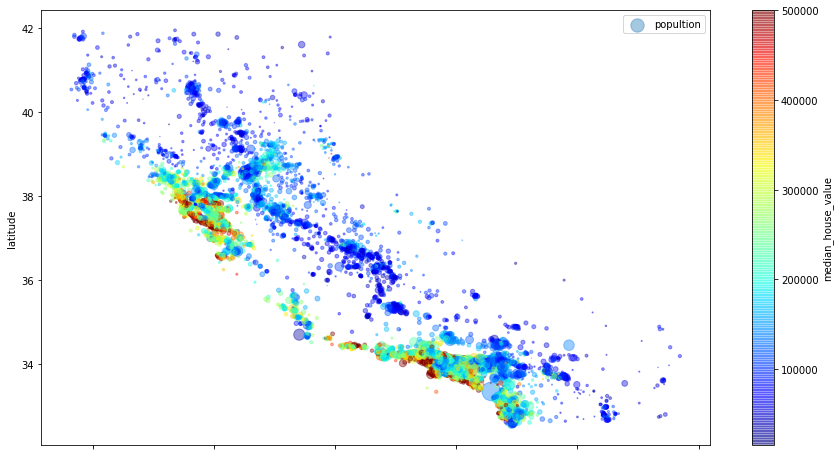
\includegraphics[scale=0.45]{img/DatasetCmap}
\caption{Example of plotting a dataframe. The latitude is plotted over the longitude. The color tells the intensity of the output variable while the circle radius tells are related to another input variable (population).}
\label{californiaHouses}
\end{figure}

\autoref{californiaHouses} shows the prices of Californian houses using a colormap in terms of geographical position and population.
This image tells you that the housing prices are very much related to the location (e.g., close to the ocean) and to the population density, as you probably knew already. It will probably be useful to use a clustering algorithm to detect the main clusters, and add new features that measure the proximity to the cluster centres. 

\subsection{Interpretation of scatter plot}
\label{scatterplot}
This method is important: it gives an idea of which variable are related: if the graph looks uniform then maybe there is no relation. On the contrary other, other patterns might be visible. For example, from \autoref{scatter_img} it is possible to see a strong correlation between \ti{median\_house\_value} and \ti{median\_income}.
\begin{figure}
\centering
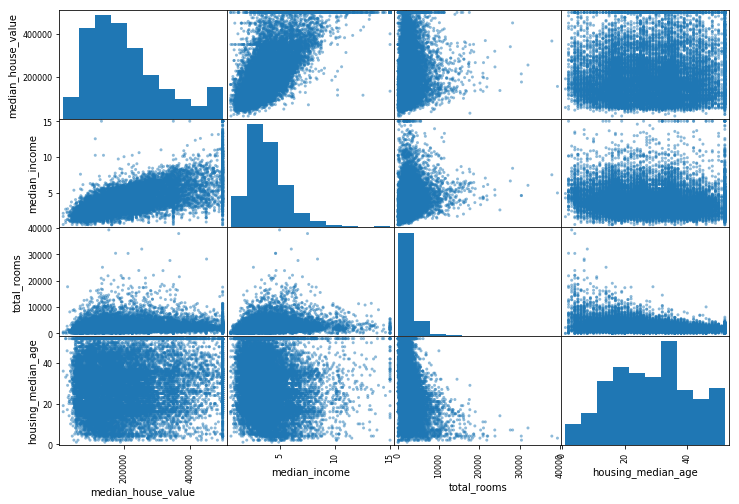
\includegraphics[scale=0.51]{img/scatterplot}
\caption{Example of scatterplot for some attributes of the California houses dataset.}
\label{scatter_img}
\end{figure}

Looking closer at it in \autoref{singleScatterPlot},
\begin{figure}
\centering
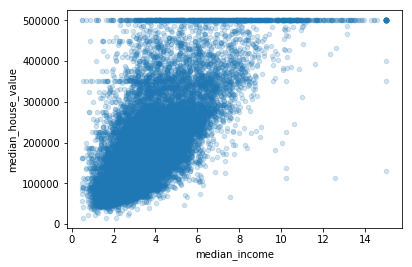
\includegraphics[scale=0.8]{img/singleScatterPlot}
\caption{Scatterplot of the attributes \ti{median\_house\_value} and \ti{median\_income}.}
\label{singleScatterPlot}
\end{figure}

\autoref{singleScatterPlot} shows these two variables are really correlated. We also notice the horizontal line at $\$500,000$ since data prices are capped.

However, there are other horizontal lines at $\$450,000$, at $\$380,000$ and maybe one at $\$280,000$. Maybe it is better to remove these districts so that the algorithm does not learn to reproduce them.

\subsection{Data manipulation}
Some values need to be properly interpreted. In the California houses data set the attribute \ti{total\_bedrooms} is the total number of rooms in a district. Rather than that, it is better to consider the approximated number of bedrooms per house, obtained by dividing the former by the total number of houses in that district. This new attribute will be more correlated to the output than the original one. Apparently houses with a lower bedroom/room ratio tend to be more expensive. 
In the same way, the number of rooms per household is also more informative than the total number of rooms in a district - obviously the larger the houses, the more expensive they are.

\subsubsection{Convert categorical values to numerical values}
Many machine algorithms work with numerical attributes and not with categorical values. It is a good idea to convert these categorical value to a numerical value. \ti{SciKit-learn} offers the \ti{LabelEncoder} class, which convert each categorical value to a number:
\begin{lstlisting}[caption=Example of usage of \ti{LabelEncoder} class]
from sklearn.preprocessing import LabelEncoder
encoder = LableEncoder();
encoder = LabelEncoder();
h_cat = h['ocean_proximity'];
h_cat_encoded = encoder.fit_transform(h_cat);
\end{lstlisting}
where \ti{ocean\_proximity} is a categorical attribute. However, there is a problem with this representation:  ML algorithms will assume that two nearby values are more similar than two distant values. Many times this is not guaranteed to be the case. To fix this issue, a common solution is to create one binary attribute for each possible categorical value. This is called \tb{one-hot encoding}, because only one attribute will be equal to 1 (hot), while the others will be 0 (cold).

\ti{SciKit-learn} provides \ti{OneHotEncoder} to convert integer categorical value into one-hot vectors. This function seems to be deprecated though.

\begin{lstlisting}[caption=Usage of \ti{ColumnTransformer}]
from sklearn.compose import ColumnTransformer
h_copy = h.copy()
ct = ColumnTransformer([("onehot",OneHotEncoder(),[h_copy.columns.get_loc('ocean_proximity')])]);
onehot = ct.fit_transform(h_copy.values).astype('int').toarray();
onehot
Out:
array([[1, 0, 0, 0, 0],
       [1, 0, 0, 0, 0],
       [0, 0, 0, 0, 1],
       ...,
       [0, 1, 0, 0, 0],
       [1, 0, 0, 0, 0],
       [0, 0, 0, 1, 0]])
\end{lstlisting}
Apparently \ti{ColumnTransformer} has no inverse so we are loosing the references to the category
We create a dataframe containing the encoding of the categorical variables and then we merge it to the original dataframe:
\begin{lstlisting}[caption=Usage of \ti{LabelBinarizer}]
from sklearn.preprocessing import LabelBinarizer
# sparse_output=True compresses the matrix not to use too much mem, 
# toarray() allows to get back the array
h_copy = h.copy();
enc = LabelBinarizer(sparse_output=True);
onehot = enc.fit_transform(h_copy['ocean_proximity']);
enc.inverse_transform(np.identity(onehot.shape[1])).reshape(-1,);
ocean_prox_df = pd.DataFrame(
		data=onehot.toarray().astype('int'), 
		columns=enc.inverse_transform(np.identity(onehot.shape[1])));

# Now we concatenate the original and one-hot encoded datafram
h_cat = pd.concat([h_copy.drop('ocean_proximity', axis=1), 
		ocean_prox_df], axis=1);
h_cat
\end{lstlisting}

Alternatively, Pandas dataframe data structure has its own simpler method \ti{pandas.get\_dummies(df.categorical\_attribute}:
\begin{lstlisting}[caption=Usage of \ti{pd.get\_dummies()}]
h_copy = h.copy();
ocean_prox_dummies = pd.get_dummies(h_copy.ocean_proximity);
h_res = pd.concat([h_copy, ocean_prox_dummies], axis=1);
h_res.drop('ocean_proximity', axis=1, inplace=True);
\end{lstlisting}

\subsection{Data cleaning}
One big problem are missing values. These can be replaced with different techniques:
\begin{itemize}
\item \tb{\ti{df.dropna(subset=["total\_bedrooms"]);}}: gets rid of the entries having null for this column(s);
\item \tb{\ti{df.drop("total\_bedrooms", axis=1);}}: gets rid of the entire attribute;
\item \tb{\ti{df["total\_bedrooms].fillna(median);}}: set the missing value to the specified value (0, mean, median).The value (\ti{median} in this case) has been computed with the training set so it must be saved
\end{itemize}

If more than one column has missing values, we can use the SciKitLearn class \ti{Imputer}. Its constructor takes as input a string parameter called \ti{strategy} that specifies the value replacement. An example is the following:
\begin{lstlisting}[caption=Usage of \ti{SimpleImputer to clean data}]
from sklearn.preprocessng import SimpleImputer
imputer = SimpleImputer(strategy="median");
h_num = h.drop('ocean_proximity', axis=1);
imputer.fit(h_num);
imputer.statistics_;
X = imputer.transform(h_num); #output is a numpy array
h_tr = pd.DataFrame(X, columns =h_num.columns)
\end{lstlisting}

\subsection{Custom Transformers}
\ti{Scikit} allows you to create your own transformers using \tb{ducking type programming style}. In ducking type, an object passed into a function must support all methods and attributes it s expected to have at runtime. The object type itself does not matter: in this sense, it is very different from inheritance. 

For \ti{Transformers}, three methods must be implemented:
\begin{itemize}
\item\ti{fit();}: this method just calculates the parameter and it is run on the training set. The parameters are saved as internal object state.
\item \ti{transform();}: it applies the transformation to a particular set of examples. it can be called right after \ti{fit()} on the training set or on the test set (on which one does not call \ti{fit})
\item \ti{fit\_transform();}: joins these two steps and is used for the initial fitting of parameters on the training set, but it also returns a transformed set. Internally, it just calls first \ti{fit()} and then \ti{transform()} on the same data.
\end{itemize}
We can get the last one for free exploiting inheritance from the base class \ti{\tb{TransformerMixin}}. By adding also \ti{\tb{BaseEstimator}} as a base class and avoiding \ti\tb{*args} and \ti\tb{*kargs} in the constructor, we will get the extra methods \ti\tb{get\_params} and ti\tb{set\_params} that will be useful for automatic hyperparameter tuning.

\begin{lstlisting}[caption=Example of how to create a custom transformer.]
from sklearn.base import BaseEstimator, TransformerMixin

rooms_ix, bedrooms_ix, population_ix, household_ix = 3, 4, 5, 6;

class CombinedAttributesAdder(BaseEstimator, TransformerMixin):
    def __init__(self, add_bedrooms_per_room=True):
        self.add_bedrooms_per_room = add_bedrooms_per_room;

    def fit(self, X, y=None):
        return self;
    
    def transform(self, X, y=None):
        rooms_per_household = X[:,rooms_ix]/X[:, household_ix];
        population_per_household = X[:,population_ix]/X[:, household_ix];
        if self.add_bedrooms_per_room:
            bedrooms_per_room = X[:,bedrooms_ix]/X[:, rooms_ix];
            return np.c_[X, rooms_per_household, population_per_household, bedrooms_per_room];
        else:
            return np.c_[X, rooms_per_household, population_per_household];
        
attr_adder = CombinedAttributesAdder(add_bedrooms_per_room=False);
h_extra_attribs= attr_adder.transform(h_copy.values);
\end{lstlisting}

\subsection{Feature scaling}
In general, inputs have very different scales. ML algorithms work better if inputs have the same scale. For this reason, they are scaled before applying the algorithm. Tow popular scaling methods are the following:
\begin{itemize}
\item \ti{\tb{min-max}} or \ti{\tb{normalization}}: values are scaled to be in range $[0,1]$. Minimum value is subtracted and then it is scaled by the maximum value. \ti{Scikit} provides \ti{MinMaxScaler} with \ti{feature\_range} property to change the range.
\item \ti{\tb{standardization}}: it subtracts the mean value (0-mean) and then divides by the variance to have a unit variance distribution. Standardization is much less affected by outliers but might be a problem for some algorithms (such as NN) expecting values to be within a given range.
\end{itemize}

\subsection{Scikit-learn transformation pipeline}
The \ti{pipeline} data structure allows to collect the transformation to be applied to the dataset. All but last estimator must be transformers, i.e., they must have the method \ti{fit\_transform}. When one calls the pipeline's \ti{fit()}method, it calls \ti{fit\_transform()} sequentially on all transformers, passing the output of each call as the parameter to the next call, until it reaches the final estimator, for which it just calls the \ti{fit()} method and then \ti{transform()}.
\begin{lstlisting}
from sklearn.pipeline import Pipeline
from sklearn.preprocessing import StandardScaler
from sklearn.impute import SimpleImputer
num_pipeline = Pipeline([('imputer', SimpleImputer(strategy='median')),
                        ('attribs_adder', CombinedAttributesAdder()),
                         ('std_scaler', StandardScaler())
                        ]);
h_num_tr = num_pipeline.fit_transform(h.drop('ocean_proximity',axis=1));
\end{lstlisting}
\subsubsection{Perform parallel transformations}
The scaling of numerical values and the transformation of categorical values to many binary attributes are independent, hence they can be performed in parallel.

Scikit provides \ti{\tb{FeatureUnion}} class. You give it a list of transformers (which can be entire transformer pipelines), and when its \ti{\tb{transform()}} method is called, it runs each transformer’s \ti{\tb{transform()}} method in parallel, waits for their output, and then concatenates them and returns the result (and of course calling its \ti{\tb{fit()}} method calls all each transformer’s \ti{\tb{fit()}} method). 

Before looking at the \ti{FutureUnion}, we needed two more pieces. First of all, each subpipeline starts with a selector transformer: it simply transforms the data by selecting the desired attributes (numerical or categorical), dropping the rest, and converting the resulting DataFrame to a NumPy array. There is nothing in Scikit-Learn to handle Pandas DataFrames, so we need to write a simple custom transformer for this task. The code in \autoref{SelectorTransfomer} does this.

\begin{lstlisting}[
caption=Transformer to select the desired attributes of a Pandas dataframe,
 label=SelectorTransfomer]
from sklearn.base import BaseEstimator, TransformerMixin

class DataFrameSelector(BaseEstimator, TransformerMixin):
    def __init__(self, attribute_names):
        self.attribute_names = attribute_names;
    def fit(self, X, y=None):
        return self;
    def transform(self, X):
        return X[self.attribute_names].values
\end{lstlisting}

Secondly, the method \ti{fit\_transform()} of \ti{LabelBinarizer} changed from SciKit-learn version 0.18 to 0.19. The problem is that now it accepts just two inputs: the instance and the array to be encoded: \ti{lb.fit\_transform(['yes', 'no', 'no', 'yes'])}, while the pipeline requires three.
We create a new class \ti{LabelBinarizerPipelineFriendly} which inherits from \ti{LabelBinarizery} overload \ti{fit\_transform()} method to accept another parameter \ti{y} that actually it is not used. The method first calls \ti{fit} and then \ti{transform()}. See \autoref{LabelBinarizerPipelineFriendly}.
\begin{lstlisting}[
caption=Custom LabelBinarizer class that can be used in a pipeline, 
label=LabelBinarizerPipelineFriendly]
class LabelBinarizerPipelineFriendly(LabelBinarizer):
     def fit(self, X, y=None):
         """this would allow us to fit the model based on the X input."""
         super(LabelBinarizerPipelineFriendly, self).fit(X)
     def transform(self, X, y=None):
         return super(LabelBinarizerPipelineFriendly, self).transform(X)

     def fit_transform(self, X, y=None):
         return super(LabelBinarizerPipelineFriendly, self).fit(X).transform(X)
\end{lstlisting}

Finally we can use \ti{FutureUnion} as in \autoref{FutureUnion}.
\begin{lstlisting}[caption=Usage of \ti{FutureUnion}, label=FutureUnion]
from sklearn.pipeline import FeatureUnion;
num_attr = list(h.drop('ocean_proximity',axis=1))
cat_attr = ['ocean_proximity']
num_pipeline = Pipeline([
                        ('selector', DataFrameSelector(num_attr)),
                        ('imputer', SimpleImputer(strategy='median')),
                        ('attribs_adder', CombinedAttributesAdder()),
                        ('std_scaler', StandardScaler())
                        ]);
cat_pipeline = Pipeline([
                        ('selector'       , DataFrameSelector(cat_attr)),
                        ('label_binarizer', LabelBinarizerPipelineFriendly())#using custom because fit_transform method changed
                        ]);
full_pipeline = FeatureUnion(
            transformer_list =[
                              ("num_pipeline", num_pipeline), 
                              ("cat_pipeline", cat_pipeline)
                              ]);
h_prepared = full_pipeline.fit_transform(h);
\end{lstlisting} 

%%%%%%%%%%%%%%%%%%%%%%%%%%%%%%%%%%%%%%%%%%%%%%%%%%%%%%%%%%
%%%%%%%%------------------------------NEW SECTION------------------------------%%%%%%%%%
%%%%%%%%%%%%%%%%%%%%%%%%%%%%%%%%%%%%%%%%%%%%%%%%%%%%%%%%%%
\newpage
\section{Linear Regression Models}
We start from the \textit{univariate linear regression}, i.e., each output consists of a single value while the input is a vector of values.

\subsection{Univariate linear regression}
Univariate means single output, i.e, $y$ is a number. The basic form is 
\begin{align}
f(X) = \beta_0 + \sum_{j-1}^p X_j \beta_j
\end{align}

The most popular estimation method for a linear model is the least square:
\begin{align}
RSS(\beta) = \sum_{i=1}^{p}  \left( y_i - f(x_i) \right)^2 = \left(\bm{y} - \bm{X}\beta\right)^T \left(\bm{y} - \bm{X}\beta\right)
\end{align}

where $\bm{X}$ is a $N \times (p+1)$ matrix with each row being an input vector, $\bm{y}$ a $N$ vector (we must have $N$ input-output pairs, in this case the output is considered mono-dimensional).

By minimizing we get:

\begin{align}
\hat{\beta} = \left( \X^T \X\right)^{-1} \X^TY
\label{OLSRegression}
\end{align}
Geometrically we are projecting $y$ onto the hyperplane spanned by $X$ and the projections is referred to as $\hat{y}$:

\begin{align}
\hat{y} =\X \left( \X^T \X\right)^{-1} \X^T Y = H Y
\end{align}
where $H$ is called the \textit{hat} matrix.


%%%%%%%%%%%%%
\subsection{Equivalence of Ordinary least squares and maximum likelihood}
We are using an additive model, assuming a Gaussian white noise:
\begin{align}
y = \beta^T \x + \epsilon \\
\epsilon \sim \CMcal{N}(0,\sigma^2)
\end{align}
Adding a constant to a Gaussian random variable is equivalent to another Gaussian random variable with the mean shifted:
\begin{equation}
Pr(y) \sim \CMcal{N}(\beta^T \x ,\sigma^2)
\end{equation}
Considering the matrix $\X$ and the output vector $\y$ representing the training set, used to estimate the coefficients, we have:
\begin{equation}
Pr(\y|\X, \beta, \sigma^2)  = \prod_{i=1}^N Pr(y_i|\x, \beta, \sigma^2) =  \prod_{i=1}^N \CMcal{N}(\beta^T \x ,\sigma^2)
\end{equation}
where we have assumed each observation is independent. A product of univariate Gaussian can be rewritten as a multivariate Gaussian:
\begin{equation}
\label{multiGauss}
\begin{aligned}
 &Pr(\y|\X, \beta, \sigma^2)  = \prod_{i=1}^N \CMcal{N}(\beta^T \x ,\sigma^2) =  \prod_{i=1}^N \frac{1}{(2\pi)^{\frac{1}{2}}\sigma}e^{-\frac{\left(y_i-\beta^T\x_i\right)^2} {2\sigma^2}}= \\
 &= \frac{1}{(2\pi)^{\frac{p}{2}}\sigma}\prod_{i=1}^N e^{-\sum_{i=1}^N \frac{\left(y_i-\beta^T\x_i\right)^2} {2\sigma^2}} = \\
 &=  \frac{1}{(2\pi)^{\frac{p}{2}}\sigma|\mathbf{I}|}e^{-\frac{1}{2}\left(\y-\beta^T\X\right)^T\left(\sigma^2 \mathbf{I}\right)^{-1}\left(\y-\beta^T\X\right)} = \CMcal{N}(\beta^T \X ,\sigma^2\mathbf{I}) 
\end{aligned}
\end{equation}
If the variables are not independent the more general form is:
\begin{equation}
\CMcal{N}(\beta^T \X ,\mathbf{\Sigma}) =\frac{1}{(2\pi)^{\frac{p}{2}}|\Sigma|^\frac{1}{2}}e^{-\frac{1}{2}\left(\y-\beta^T\X\right)^T\Sigma^{-1}\left(\y-\beta^T\X\right)}
\end{equation}

%%%%%%%%
\paragraph{Definition of likelihood}
The quantity $Pr(y|\x, \beta, \sigma^2)$ is called \textbf{likelihood} and tell us how much it is likely the outcome $y_i$ in the dataset given the input $\x$ and the parameters.

A different approach to find a model that fits the data is to maximize the \textit{likelihood} of the whole dataset:
\begin{equation}
L = Pr(\y|\X, \beta, \sigma^2)  = \frac{1}{(2\pi)^{\frac{p}{2}}|\Sigma|^\frac{1}{2}}e^{-\frac{1}{2}\left(\y-\beta^T\X\right)^T\Sigma^{-1}\left(\y-\beta^T\X\right)}
\end{equation}

Actually maximizing the likelihood is equivalent to maximizing its logarithmic, the \textit{log-likelihood}:
\begin{equation}
\begin{aligned}
&\log L = \sum_{i=1}^N \log\left[\frac{1}{(2\pi)^{\frac{1}{2}}\sigma}e^{-\frac{\left(\y_i-\beta^t \x_i\right)^2} {2\sigma^2}}\right]\\
&=\sum_{i=1}^N -\frac{1}{2}\log2\pi -\log \sigma -\frac{\left(y_i-\beta^T\x_i\right)^2} {2\sigma^2} =\\
&= -\frac{1}{2}\log2\pi -\log \sigma -\frac{1}{2\sigma^2} \sum_{i=1}^N\left(y_i-\beta^T\x_i\right)^2
\end{aligned}
\end{equation}
As already done for OLS, taking the derivative w.r.t. $\beta$ and setting it to $0$:
\begin{equation}
\begin{aligned}
&\frac{\partial \log L}{\partial \beta} = -\frac{1}{2\sigma^2} \left(-2\right) \left(\y_i-\beta^T\x_i\right) = 0 \\
&\Rightarrow \left(\y-\beta^T\X \right)= 0 \Rightarrow \beta = \HM \y
\end{aligned}
\end{equation}

This is the same solution of the OLS: the two models are equivalent.

\textbf{The two models are equivalent assuming a normal distribution}.

\subsection{Expectation of the parameter estimation: unbiased estimator}
Computing the expectation of $\hat{\beta}$:
\begin{equation}
\begin{aligned}
&\E_{Pr(\y|\X,\beta, \sigma^2)}\left[ \hbe\right]= \sum \hbe Pr(\y|X, \beta, \sigma^2) =\\
&= \HM \sum \y Pr(\y |X, \beta, \sigma^2)  = \\
&=\HM \E_{Pr(\y | \X,\beta, \sigma^2)} \left[ \y\right] = \\
&= \HM \X \beta = \beta
\end{aligned}
\end{equation}

This is an \textbf{unbiased estimator}.

Now let us calculate the covariance matrix:
\begin{equation}
\begin{aligned}
&\Cov \left[\hb \right] = \\
&=\E_{Pr(\y|\X,\beta, \sigma^2)}\left[ \left( \hb -\E_{Pr(\y|\X,\beta, \sigma^2)}\left[ \beta\right] \right) \left( \hb -\E_{Pr(\y|\X,\beta, \sigma^2)}\left[ \beta\right] \right)^T\right] = \\
&=\E_{Pr(\y|\X,\beta, \sigma^2)}\left[ \left( \hb - \beta \right) \left( \hb - \beta \right)^T\right] =\\
&=\E_{Pr(\y|\X,\beta, \sigma^2)}\left[ \hb\hb^T\right] -\beta\beta^T\end{aligned}
\end{equation}
and
\begin{equation}
\begin{aligned}
&\E_{Pr(\y|\X,\beta, \sigma^2)}\left[ \hb\hb^T\right] = \\
&=\E_{Pr(\y|\X,\beta, \sigma^2)} \left[ \left( \HM \y\right)\left( \HM \y\right)^T\right] = \\
& = \HM\E_{Pr(\y|\X,\beta, \sigma^2)} \left[   \y  \y^T\right] \X \inv
\end{aligned}
\end{equation}
and recalling from \autoref{multiGauss} $Pr(\y) \sim \CMcal{N}(\beta^T \X ,\sigma^2 \mathbf{I})$
\begin{equation}
\begin{aligned}
&\Cov\left[ \y\right]=\sigma^2 \mathbf{I} =\\
&=\E_{Pr(\y|\X,\beta, \sigma^2)}\left[ \y\y^T\right]  - \E_{Pr(\y|\X,\beta, \sigma^2)}\left[ \y\right]\E_{Pr(\y|\X,\beta, \sigma^2)}\left[ \y^T\right]\\
\end{aligned}
\end{equation}

Rearranging
\begin{equation}
\begin{aligned}
&\Rightarrow \E_{Pr(\y|\X,\beta, \sigma^2)}\left[ \y\y^T\right] = \sigma^2 \mathbf{I} +\E_{Pr(\y|\X,\beta, \sigma^2)}\left[ \y\right]\E_{Pr(\y|\X,\beta, \sigma^2)}\left[ \y^T\right] =\\
&=\sigma^2 \mathbf{I} +\E_{Pr(\y|\X,\beta, \sigma^2)}\left[ \X\beta\right]\E_{Pr(\y|\X,\beta, \sigma^2)}\left[ \beta^T\X^T\right] =\\
&= \sigma^2 \mathbf{I} +\X\beta \beta^T\X^T
\end{aligned}
\end{equation}

Substituting:

\begin{equation}
\begin{aligned}
&\E_{Pr(\y|\X,\beta, \sigma^2)}\left[ \hb\hb^T\right] = \HM \left(\sigma^2 \mathbf{I} +\X\beta \beta^T\X^T\right)X \inv   = \\
 &=\sigma^2 \inv 
\end{aligned}
\end{equation}

and finally variance-covariance matrix of the least square parameters is 
\begin{equation}
\begin{aligned}
&\Cov\left[ \hb\right]=  \inv  \sigma^2
\end{aligned}
\end{equation}
 
\begin{align}
Var(\hat{\beta}) = (\X^T\X)^{-1} \sigma^2
\end{align}

\subsection{Noise variance estimation}
We can find an estimation of the noise variance from the maximum likelihood model using the same procedure used to find the parameters, i.e., taking the derivative and equating it to $0$:
\begin{equation}
\begin{aligned}
\label{varErr}
&\frac{\partial \log L}{\partial \sigma} = \sum_{i=1}^N-\frac{1}{\sigma} +\frac{1}{\sigma^3} \left(y_i - \x_i^T\beta\right)^2 = 0 \Rightarrow \frac{N}{\sigma} +\frac{1}{\sigma^3}  \sum_{i=1}^N\left(y_i - \x^T\beta\right)^2 = 0\\
&\Rightarrow \hat{\sigma^2} = \frac{1}{N}\sum_{i=1}^N\left(y_i - \x_i^T\beta\right)^2 
\end{aligned}
\end{equation}
This can be re-expressed as
\begin{equation}
\begin{aligned}
&\Rightarrow \hat{\sigma^2} = \frac{1}{N}\sum_{i=1}^N\left(y_i - \x^T\hb\right)^2  = \frac{1}{N}\sum_{i=1}^N\left(y_i - \x_i^T\HM\y\right)^2 = \\
&= \frac{1}{N}\left(\y - \X\HM\y\right)^T\left(\y - \X\HM\y\right) = \\
&=\y^T\y  - 2 \y^T  \X\HM\y + \y^T \X \cancel{\inv} \cancel{\X^T \X}\HM\y = \\
&=\y^T\y  - \y^T  \X\HM\y  = \left(\y^T\y - \y^T\X\hb \right)
\end{aligned}
\end{equation}

Taking the expectation w.r.t. $Pr(\y|\X,\beta, \sigma^2)$:
\begin{equation}
\begin{aligned}
&\E_{Pr(\y|\X,\beta, \sigma^2)} \left[\hs\right] = \frac{1}{N}\E_{Pr(\y|\X,\beta, \sigma^2)} \left[\y^T\y - \y^T\X\hb \right] =\\
&=\frac{1}{N}\E_{Pr(\y|\X,\beta, \sigma^2)} \left[\y^T\y \right] - \frac{1}{N}\E_{Pr(\y|\X,\beta, \sigma^2)} \left[\y^T\X\HM \y \right] 
\end{aligned}
\end{equation}

Suppose $\mathbf{t} \sim  \CMcal{N}\left(\mathbf{\mu}, \mathbf{\Sigma} \right)$, then $\E_{p(\mathbf{t})} \left( \mathbf{t^TAt}\right)= \Tr(\mathbf{A\Sigma})+\mathbf{\mu^TA\mu}$ with $\mu = \X\beta$

\begin{equation}
\begin{aligned}
&\E_{Pr(\y|\X,\beta, \sigma^2)} \left[\hs\right] =\frac{1}{N}\E_{Pr(\y|\X,\beta, \sigma^2)} \left[\y^T\y \right] +\\
&- \frac{1}{N}\E_{Pr(\y|\X,\beta, \sigma^2)} \left[\y^T\X\HM \y \right]  = \\
&= \frac{1}{N}\E_{Pr(\y|\X,\beta, \sigma^2)} \left[\y^T\mathbf{I}_N\y \right] +\\
&- \frac{1}{N}\E_{Pr(\y|\X,\beta, \sigma^2)} \left[\y^T\X\HM \y \right]  = \\
&=\frac{1}{N}\left(\Tr\left(\sigma^2\mathbf{I}_N\right) +\beta^T\X^T\X\beta \right) + \\
&- \frac{1}{N}\left(\Tr\left[\sigma^2\X\HM\right] +\beta^T\X^T\X\HM\X\beta  \right) =\\
&= \frac{1}{N}\left(N\sigma^2 +\beta^T\X^T\X\beta \right) - \frac{1}{N}\left(\sigma^2\Tr\left[\X\HM\right] +\beta^T\X^T\X\beta  \right) =\\
&= \sigma^2 +\cancel{\frac{1}{N}\beta^T\X^T\X\beta} -\frac{\sigma^2}{N}\Tr\left[\X\HM\right] \cancel{-\frac{1}{N}\beta^T\X^TX\beta} = \\
&=\sigma^2 -\frac{\sigma^2}{N}\Tr\left[\HM\X\right] = \sigma^2 -\frac{\sigma^2}{N}\Tr\left[\mathbf{I}_p\right]  \\
&\Rightarrow \E_{Pr(\y|\X,\beta, \sigma^2)} \left[\hs\right] = \sigma^2 \left( 1 - \frac{p}{N}\right)
\end{aligned}
\end{equation}
where lastly we have used the product property of the trace (see \autoref{trace}).

Normally $p<N$ hence the estimate of the variance is smaller than the true variance, so this estimator is \textbf{biased}. The estimate gets closer to the real value when $p/N$ is small, i.e., assuming $p$ is fixed, increasing the samples used. 

This result might be strange. First of all notice from \autoref{varErr} that the closer the model gets to the data, the smaller $\hs$. By definition the parameter estimates are the ones that minimise the noise and hence $\hs$. As a consequence, when using the true parameters we would get equal or higher variance.

To estimate the true variance we can use the following formula:
\begin{align}
\hat{\sigma}^2 = \frac{1}{N-p-1}\sum_{i=1}^{N}(y_i-\hat{y}_i)^2
\end{align}
$N-p-1$ makes this estimation unbiased i.e., $\frac{1}{N-p-1}\E[\hat{\sigma}^2] =\sigma^2$.

\subsection{Interpretation of covariance}
Consider a covariance matrix of size $2\times 2$ for a two parameter model (i.e., a line on the plane) and suppose the first diagonal element, corresponding to the variable $\hb_0$ is much bigger than the second one corresponding to $\hb_1$. This means that we can change $\hb_0$ a little without affecting too much the model. On the contrary if the variance is small, small changes will affect significantly the model. Sometimes this happens when one variable has a much higher absolute value.

If the values on the off-diagonals are negative, then when increasing one coefficient i.e., $\hb_0$, the other must be decreased to have the line to pass as close as possible to all points. For example in $2D$, increasing $\hb_0$ reduces the coefficient value: if it is positive, the line will be "more horizontal", if negative it becomes steeper, "more vertical".
\subsection{Z-score}
Let us assume data were really generated by a linear model but were corrupted by Gaussian noise with $0$ mean and variance $\sigma^2$:

\begin{align}
Y = \beta_0 +\sum_i^p \beta_i X_i + \epsilon
\end{align} 
where $\epsilon \sim \CMcal{N}(0,\sigma^2)$.
The estimated parameters will still be a normal distribution:

\begin{align}
\label{parameterVar}
\hat{\beta} \sim \CMcal{N}(\beta,  (\X^T\X)^{-1} \sigma^2)
\end{align}

\begin{definition}{\textbf{Z-score}}
A Z-score, is a numerical and statistical measurement of a value's relationship to the mean (average) of a group of values, measured in terms of standard deviations from the mean. If a Z-score is 0, it indicates that the data point's score is identical to the mean score. A Z-score of 1.0 would indicate a value that is one standard deviation from the mean. Z-scores may be positive or negative, with a positive value indicating the score is above the mean and a negative score indicating it is below the mean. Z-scores are measures of an observation's variability

\begin{align}
z_j=\frac{x - \mu}{\sigma}
\end{align}

In machine learning the z-value is generally intended as the regression coefficient divided by its standard error. It is also sometimes called the z-statistic. If the z-value is too big in magnitude (i.e., either too positive or too negative), it indicates that the corresponding true regression coefficient is not $0$ and the corresponding X-variable matters. A good rule of thumb is to use a cut-off value of $2$ which approximately corresponds to a two-sided hypothesis test with a significance level of $\alpha=0.05$.

Z-values are computed as the test statistic for the hypothesis test that the true corresponding regression coefficient $\beta_j$ is $0$. In hypothesis testing, one assumes the null hypothesis is true, and then see if data provide evidence against it. So in this case, $\beta$ is assumed to be  $0$. That is, the expectation of the fitted regression coefficient $\hat{\beta}$ is assumed to be $0$:

\begin{align}
z_j =\frac{\hat{\beta}_j}{\hat{\sigma} \sqrt{v_j}}
\end{align}
where the denominator is the standard deviation (root square of the variance) of the parameter (from \autoref{parameterVar}) with $v_j$ being the diagonal element of $(X^TX)^{-1}$.
\end{definition}

Being the parameters normally distributed by assumption, the standard error tells you how far on average sample parameters tend to deviate from the mean population parameter, i.e., from the true parameter $\be$.

\begin{theorem}[\textbf{The Gauss-Markov theorem}]
Among all linear unbiased estimators, the least square estimates of the parameters are the ones having smallest variance and consequently from \autoref{biasVar} is the one with the smallest mean squared error (the bias-squared term for unbiased estimator is by definition $0$).
\begin{proof}
Let $\hat{\beta} = Cy$ be another linear estimator of $\beta$ with $C = (X^TX)^{-1}X^T+D$
\begin{align}
&\E\left[ \hat{\beta} \right] = \E\left[ Cy \right] = \E\left[\left(\left(X^TX\right)^{-1}X^T+D\right) \left( X\beta+\epsilon\right)\right] =\\
& = \left(\left(X^TX\right)^{-1}X^T X\beta +DX\beta\right) +\cancel{\left(\left(X^TX\right)^{-1}X^T  +D\right) \E[\epsilon]}=\\
& = \left(\beta +DX\beta\right) = \left( I +DX\right) \beta\\
\end{align}
where $ \E[\epsilon] = 0$.

To be an unbiased estimator $DX = 0$, then

\begin{equation}
\begin{aligned}
\Var(\hat{\beta}) &= \Var(Cy) = C\Var(y) C^T = \sigma^2 CC^T = \\
&= \sigma^2 \left( \left(X^T X\right)^{-1}X^T +D \right)    \left( \left(X^T X\right)^{-1}X^T+D\right)^T =\\
&= \sigma^2 \left( \left(X^T X\right)^{-1}X^T +D \right)    \left( X \left(X^TX\right)^{-1} + D^T \right)  =\\
&= \sigma^2 (  \cancel{\left(X^TX\right)^{-1}}\cancel{X^T X}   \left(X^TX\right)^{-1} +  \left(X^T X\right)^{-1}X^TD^T                          +\\
&\quad + D X \left(X^TX\right)^{-1} +DD^T) =\\
&= \sigma^2 (  \cancel{\left(X^TX\right)^{-1}}\cancel{X^T X}   \left(X^TX\right)^{-1} +  \left(X^T X\right)^{-1}\left( DX \right)^T                          +\\
&\quad + D X \left(X^TX\right)^{-1} +DD^T) \\
DX=0 \\\Rightarrow \Var(\tilde{\beta}) &= \sigma^2 \left( \left(X^TX\right)^{-1} +  \cancel{\left(X^T X\right)^{-1}\left( DX \right)^T }  + \cancel{D X \left(X^TX\right)^{-1} }+DD^T\right) \\
\Var(\tilde{\beta}) &= \Var(\hat{\beta})  + \sigma^2DD^T
\end{aligned}
\end{equation}

\end{proof}
\end{theorem}
\subsection{Orthogonalization}
Normally inputs are not perpendicular but can be orthogonalized. The goal is to define a new orthogonal basis for the data. The procedure, named \textbf{Grand-Schmidt procedure} consists of building up a new matrix of our data starting from $\X$ matrix, whose columns are orthogonal. The new columns are obtained as linear combinations of the columns of $\X$, hence they span the same space. The procedure can be summarized in the following steps:
\begin{algorithm}[!ht]
initialize $z_0=x_0=\mathbf{1}$ where $\mathbf{1}$ is a vector of all ones\;
For $j=1,\cdots, p$ regress $x_j$ on $z_0,\cdots, z_{p-1}$ to produce the coefficients $\hat{\gamma}_{lj}= \frac{\langle z_l , x_j\rangle}{\langle z_\ell , z_\ell\rangle}$ for $l=0,\cdots, j-1$\;
Calculate the residual vectors as $z_j = x_j - \sum_{k=0}^{j-1} \hat{\gamma}_{kj}z_k$\;
Regress $\mathbf{y}$ on the residual $z_p$ to get the estimate $\hat{\beta}_p = \frac{\langle z_p, y\rangle}{\langle z_p , z_p\rangle}$
\end{algorithm}
The first row of $\Gamma$ is $(1, 0, 0,\cdots 0)$ because of the initialization of
$x_0, z_0$ as vectors of ones in the first step of the algorithm. From a mathematical point of view we are building orthogonal vectors that describe the same space of the one described by the column of $\X$. To start the orthogonalization procedure, we take the first column vector of $\X$ as it is, in other words, the first direction
remains the same and we are not rescaling the vector. At the second step, we take the second column vector of $\X$, we project it onto $z_0$ to get the coefficient $\Gamma_{1,0}$, and then we get the second direction orthogonal to the first one as the vectorial difference of the column of $\X$ and its projection.

When inputs are correlated, the residual will be close to zero generating instabilities in the coefficients $\hat{\beta}_j$ and the z-score will be small.

The algorithm in matrix form is
\begin{align*}
\mathbf{X = Z\Gamma}
\end{align*}
where $z_j$ are the column vectors of $Z$ and $\Gamma$ is upper triangular. Introducing the diagonal matrix $D$ with $j$-th diagonal element $D_{jj}=||z_j||$ we get:

\begin{equation}
\mathbf{X = ZD^{-1}D\Gamma = QR}
\end{equation}
where $Q$ is an orthogonal, $Q^TQ=I$, $ N\times(p+1)$ matrix and $R$ is a $(p+1)(p+1)$ upper triangular matrix. The $Q$ matrix contains an orthonormal basis spanning the same space spanned by $\X$. The $R$ matrix contains the coefficients that multiply the orthonormal basis to get back the original matrix $X$. Consider the first step of the orthogonalization procedure. It takes the first column of $\X$ and just rescales it to have norm $1$. So to get back the first column of vector just a coefficient is needed. Hence, the first column of $R$ is just a column of $0$s except the first term. Then the second column of $\X$ is projected onto $q_1$ to get the first multiplier: this is the first element of the second column of $R$.The residual is perpendicular to $q_1$ and can be used as second axis after normalization: the scale factor is the second element of the column of $R$, all the other elements will be $0$. That is why $R$ is upper triangular.

The least square solution becomes 
\begin{equation}
\begin{aligned}
\hat{\beta} &= R^{-1}Q^Ty\\
\hat{y} &= QQ^Ty
\end{aligned}
\end{equation}

\subsection{Multivariate output}
We can rewrite the equation in matrix form:

\begin{equation}
Y = XB + E
\end{equation}
where $Y$ is  a $N\times K$ matrix, $X$ is $N\times(p+1)$, $B$ is $(p+1)\times K$, $E$ has the same dimensions of $Y$.
The root squared error is 
\begin{equation}
\begin{aligned}
RSS(B) &= \sum_{k=1}^K\sum_{i=1}^N\left(y_{ik}-f(x_i)\right)^2 = tr \left[  \left( Y-XB\right)^T\left( Y-XB\right) \right]	\\
\Rightarrow B &= \left( X^TX\right)^{-1}X^TY
\end{aligned}
\end{equation}
Multiple outputs do not affect one another's least square estimates.

\subsection{Subset selection}
Least square estimates sometimes show low bias but high variance resulting in a non-satisfactory prediction accuracy. This can be improved by setting some coefficients to $0$ to sacrifice a little of bias to reduce significantly the variance.

Other times it is useful to reduce the input dimensionality for easiness of interpretation or for computation purposes.

\subsubsection{Best subset selection}
This algorithm finds for each $k \in {0,1,2,	\cdots p}$, the subset of size $k$ that gives the smallest residual sum of squares. Note that if a variable is in the best subset of size $m$, it might not be in the subsets of larger size (and of course neither in the smallest ones).

\subsubsection{Forward stepwise selection}
Searching for all the subsets is too computationally intensive (and infeasible for $p>40$). The \textit{forward stepwise} algorithm starts with the intercept and then sequentially adds to the model the predictor that most improves the fit. $QR$ decomposition can be exploited to choose the next candidate. Particularly, we start from the intercept so that the first normal vector, $q_1$ is derived from the column of $1$s by normalization. At each step we will have $q$ vector features that have already been used to form a partial basis $Q_q$ of size $n\times q$, and the remaining $p-q$ features that still must be exploited. For each remaining feature, calculate the residual:

\begin{equation}
r_k  = x_k - \left(x_k^T Q_qQ_q^T\right)^T = x_k - Q_qQ_q^Tx_k
\end{equation}
The possible orthonormal vector is the normalized residual, $\tilde{q}_{q+1}$. The column $x_k$ to be considered to form the new direction $q_{q+1}$ is the one for which the product $y^T \tilde{q}_{q+1}$ is maximized. From this best candidate and the matrix $Q_{q}$, we build the matrix $Q_{q+1}$:
\begin{equation}
Q_{q+1} = \left[Q_{q}, q_{q+1}\right]
\end{equation}
The $R$ matrix must be updated too: first a row of zeros is appended to the end. Then a column containing the coefficients is obtained by projection of the vector $x_k$ onto $Q_{q+1}$:

\begin{equation}
  R_{q+1} = 
  \left[ \begin{array}{ *{5}{c} }
    & & &\text{\Large{$|$}}  &\\
    & &&\text{\Large{$|$}} &  \\
    \multicolumn{3}{c}
      {\raisebox{\dimexpr\normalbaselineskip+.3\ht\strutbox-.3\height}[0pt][0pt]
        {\scalebox{2}{$R_q$}}} &\text{\Large{$|$}}& {\raisebox{\dimexpr\normalbaselineskip+.2\ht\strutbox-.2\height}[0pt][0pt]
        {\scalebox{2}{$Q_{q+1}^Tx_k$}}}\\
    0 & \cdots & 0&\text{\Large{$|$}} &
  \end{array} \right] =   \left[ \begin{array}{ *{5}{c} }
    & & &\text{\Large{$|$}}  & \langle{q_1, x_k\rangle}\\
    & &&\text{\Large{$|$}}  & \langle{q_2, x_k\rangle}\\
    \multicolumn{3}{c}
      {\raisebox{\dimexpr\normalbaselineskip+.3\ht\strutbox-.3\height}[0pt][0pt]
        {\scalebox{2}{$R_q$}}} &\text{\Large{$|$}}&\vdots\\
    0 & \cdots & 0&\text{\Large{$|$}} &\langle{q_{q+1}, x_k\rangle}
  \end{array} \right]
\end{equation}
This algorithm is a greedy sub-optimal algorithm. Statistically it will have lower variance but higher bias.

\subsubsection{Backward stepwise selection}
\textit{Backward stepwise} selection starts with the full model and sequentially removes the predictor having least impact on the model, i.e., having the smallest $Z-score$.

\textbf{Note}: this algorithm can only be applied when $N>p$ while \textit{forward stepwise} can always be used.

\subsubsection{Implementations}
[From ESLII pg. 60]
Some software packages implement hybrid stepwise-selection strategies that consider both forward and backward moves at each step, and select the "best" of the two. For example in the R package the step function uses the AIC criterion for weighing the choices, which takes proper account of the number of parameters fit; at each step an add or drop will be performed that minimizes the AIC score.

Other more traditional packages base the selection on \textit{F}-statistics, adding "significant" terms, and dropping "non-significant" terms. These are out of fashion.

\subsubsection{Forward stagewise regression}
As forward stepwise, it starts with the intercept. At each step the algorithm identifies the variable most correlated with the residual and for the chosen variable it computes the linear regression coefficient using the residual (instead of the full target) itself and just the chosen variable (instead of the full input matrix). This scalar value is added to the old value of the coefficient.

This is continued till none of the variables have correlation with the residual. The correlation can be calculated as a scalar product, it must be remembered to use absolute values when comparing correlations.

At each step only one coefficient is updated and the update might not give the final coefficient so that the number of steps is bigger than $p$. This slow-fitting pays in high dimensions.

\textbf{Note}: forward stagewise is very competitive in 

\subsection{Shrinkage methods}
Subset selection methods either keep or remove a predictor. It has higher variance. Shrinkage or regularization methods are more continuous. They force the model to keep the weights as small as possible.


\subsubsection{Ridge regression}
Ridge regression shrinks the coefficients by imposing a penalty on their size.	 The ridge coefficients minimize a penalized residual sum of squared errors
\begin{equation}
\label{bridge}
\hat{\beta}^{ridge} = \argmin{\beta} \Bigg\lbrace \sum_{i=1}^N \left( y_i -  \beta_0 - \sum_{j=1}^p x_{ij} \beta_j\right)^2+ \lambda \sum_{j=1}^p \beta_j^2 \Bigg\rbrace
\end{equation}

where $\lambda$ is a parameter controlling the amount of shrinkage: the bigger the value the greater the amount of shrinkage. This concept is also used in the Neural Networks. Another way to express \autoref{bridge} is the following:
\begin{equation}
\begin{aligned}
&\hat{\beta}^{ridge} = \argmin{\beta} \Bigg\lbrace \sum_{i=1}^N \left( y_i -  \beta_0 - \sum_{j=1}^p x_{ij} \beta_j\right)^2 \Bigg\rbrace\\
&\text{subject to} \sum_{j=1}^p \beta_j^2 \le t
\end{aligned}
\end{equation}
where there is a one-to-one correspondence between $\lambda$ and $t$. Note that the penalization term does not consider $\beta_0$ otherwise the procedure will depend on the chosen origin for $Y$.

This algorithm solves the problem of high variance in case of correlated inputs when big coefficients of correlated variables can be cancelled out. With a constraints on the coefficients this problem is alleviated.

The coefficients are not preserved when the input is scaled. Generally inputs are standardized before applying the algorithm.

\begin{align}
RSS(\lambda, \beta)       &= \left( y - X \beta \right)^T \left( y - X\beta \right) + \lambda \beta^T \beta \\
\hat{\beta}^{ridge} &= \left( X^TX + \lambda I \right)^{-1} X^Ty
\end{align}

Now even if $X$ is not full rank, the problem is non singular (the inverse exists).
In case of orthonormal inputs, the ridge coefficients are the same of least square but scaled: $\hat{\beta}^{ridge}  = \frac{\hat{\beta}}{1+\lambda}$.

The parameter $\lambda$ can also be derived assuming a prior distribution $y_i  \sim  \CMcal{N}\left( \beta_0+x_i^T\beta, \sigma^2\right)$ and the parameters $\beta_j$ are distributed as $\CMcal{N}\left( 0, \tau^2\right)$. Then from \autoref{bridge} $\lambda = \frac{\sigma^2}{\tau^2}$.

Applying the SVD decomposition of the matrix $\mathbf{X =  UDV^T}$ where $X$ is $N\times p$, $U$ is $N\times p$and $V$ is $p\times p$, the latter two both orthogonal with the columns of $U$ spanning the column space of $X$ and the columns of $V$ spanning the row space of $X$. $D$ is a $p\times p$ diagonal matrix with the elements $d_1\ge d_2 \ge \cdots \ge d_p\ge 0$ called singular value decomposition of $X$. If any $d_j = 0$ then $X$ is singular.

The least squares equation can be rewritten as 
\begin{equation}
\mathbf{X}\hat{\beta}^{ls}  = \mathbf{X\left( X^TX\right)}^{-1}\mathbf{X^Ty} = \mathbf{UU^T}y
\end{equation}

In case of the ridge regression, the coefficients are
\begin{equation}
\begin{aligned}
\mathbf{X}\hat{\beta}^{ridge}  &= \mathbf{X}\left( \mathbf{X^TX} +\lambda \mathbf{I} \right)^{-1}\mathbf{X^Ty} = \mathbf{UU^Ty} =\\
&= \sum_{j-1}^p \mathbf{u}_j \frac{d_j^2}{d_j^2+\lambda} \mathbf{u_j}^Ty
\end{aligned}
\end{equation}
where $u_j$ are the column vectors. So ridge regression first computes the coordinates of $y$ with respect to the orthonormal basis $\mathbf{U}$, it then shrinks those coordinates since $\lambda\ge0$. A greater amount of shrinkage is applied to the coordinates of basis vector with smaller $d_j$, corresponding to elements with small variance.

\subsubsection{Lasso regression}
The lasso regression is similar to ridge regression but it uses a $L_1$ penalization instead of $L_2$.
\begin{equation}
\label{blasso}
\hat{\beta}^{lasso} = \argmin{\beta} \Bigg\lbrace \sum_{i=1}^N \left( y_i -  \beta_0 - \sum_{j=1}^p x_{ij} \beta_j\right)^2+ \lambda \sum_{j=1}^p |\beta_j| \Bigg\rbrace
\end{equation}
or equivalently
\begin{equation}
\begin{aligned}
&\hat{\beta}^{lasso} = \argmin{\beta} \Bigg\lbrace \sum_{i=1}^N \left( y_i -  \beta_0 - \sum_{j=1}^p x_{ij} \beta_j\right)^2 \Bigg\rbrace\\
&\text{subject to} \sum_{j=1}^p |\beta_j| \le t
\end{aligned}
\end{equation}
If $t>t_0= \sum_1^p |\beta_j|$ where $\beta_j$ are the least square coefficients, then the lasso coefficients are the same of the least squares ones. If $t=t_0/2$ then the least square coefficients are shrunk by $50\%$ on average. Making $t$ sufficiently big will cause some of the coefficients to be exactly $0$.

In \autoref{ridge_lasso}, the blue areas show the constraints for the estimates of ridge and lasso regressions, while the ellipses are contours of the residual sum of squares, centred at $\beta^{ls}$, in case of only two coefficients. For the lasso one of the coefficients is $0$ when it hits one of the corner. In higher dimensions the figure becomes a rhomboid with many corners (and faces) so it becomes easy to hit a corner. 
\begin{figure}
\centering
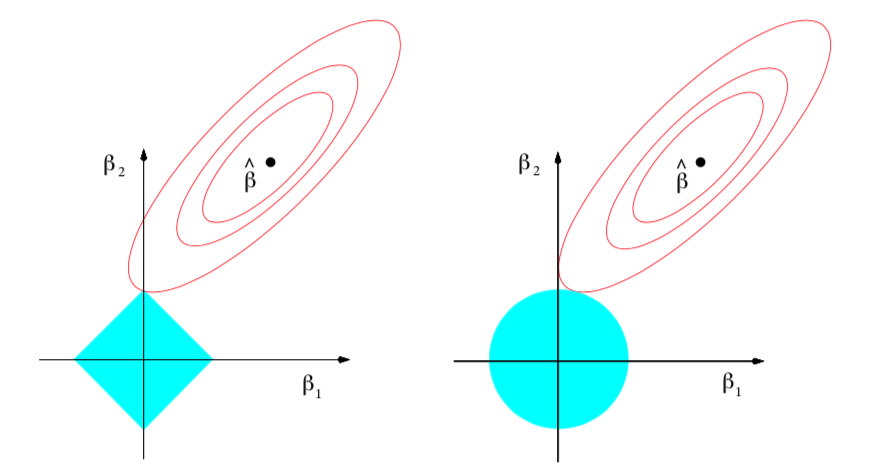
\includegraphics[scale=0.4]{img/ridge_lasso}
\caption{Constraints of Ridge and Lasso regressions.}
\label{ridge_lasso}
\end{figure}

Also other penalization factors can be chosen, \autoref{penalization}

\begin{figure}
\centering
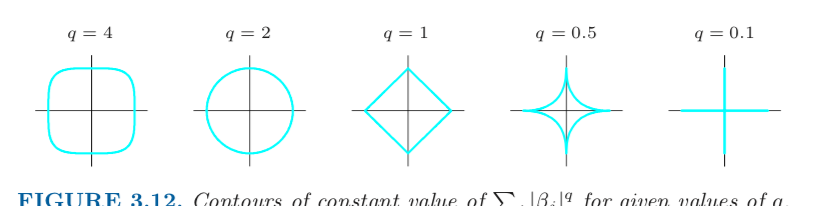
\includegraphics[scale=0.4]{img/penalization}
\caption{Shapes of different penalization factors.}
\label{penalization}
\end{figure}

\subsubsection{Least angle regression}
It is similar to forward stepwise. At first it identifies the variable most correlated with the response but instead of fitting it completely, it moves the variable toward its least squares value. As soon as another value gets correlated to the residual as the previous variable, the process is paused. The second variable joins the active set and their coefficients are moved together in a way that keeps their correlations tied and decreasing. The process is continued until all the variables are in the model.
\begin{algorithm}[!ht]
standardize the predictors to have $0$ mean and unit norm\;
$\mathcal{A}_k\leftarrow 0$\;
$r\leftarrow y-\bar{y}$, $\beta_i=0$ for $i\ne0$\;
\While {$|\mathcal{A}_k|<p$}{
find the predictor most correlated to $r$\;
insert the predictor in the active set $\mathcal{A}_k$\;

move the coefficients of the predictors in the active set to the direction defined by their joint least squares coefficient of the current residual, i.e.,
\begin{equation}
\delta_k = \left( X_{\mathcal{A}_k}^T X_{\mathcal{A}_k}\right)^{-1} X_{\mathcal{A}_k}^T r_k
\end{equation}
(where $\mathcal{A}_k$ is the current active set of variables) until some other competitor $x_\ell$ has as much correlation with the current residual\;
$r_k\leftarrow y - X_{\mathcal{A}_k}\beta_{\mathcal{A}_k}$
}
\end{algorithm}
After $min(N-1,p)$ steps we we arrive at the full least squares solution.
The coefficient profile evolves as
\begin{equation}
\beta_{\mathcal{A}_k} =  \beta_{\mathcal{A}_k} + \alpha \delta_k
\end{equation}

If to the LAR algorithm we add the following rule i.e.,

\textit{If a non-zero coefficient hits $0$, drop its variable from the active set of variables and recompute the current joint least squares direction.}

we get the same coefficient path of the lasso and this is called LAR(lasso). So this become an efficient solution to compute the Lasso problem, especially with $N>>p$ since Lasso can take more than $p$ steps while LAR require $p$ steps and it is efficient since it requires the same complexity as that of a single least squares fit using the $p$ predictors.

\subsection{Derived input directions methods}
When a large number of inputs is present, often there is a high correlation among them. In this case is convenient to regress on a new set inputs obtained form a linear combination of the original input.

\subsubsection{Principal component analysis}
The first input must be standardized since this analysis depends on the scaling. The principal components are defined as  	
\begin{equation}
z_i = X v_i
\end{equation}
where $v_i$ are the column vectors of $V$ from the SVD decomposition of $X=U\Sigma V^T$ (recall that $z_m$ are orthogonal)(\autoref{SVD}). The algorithm then regress $X$ on $z_1,\cdots, z_M$ for $M\le p$ and we have:

\begin{equation}
\hat{y}^{pcr}_{(M)} = \bar{y}\mathbf{1} + \sum_{m=1}^M \hat{\theta}_m z_m
\end{equation}
where $\hat{\theta}_m = \langle z_m, y\rangle/\langle z_m, z_m \rangle$. Since $z_m$ are linear combination of the original predictors $x_j$, we can express the solution as 

\begin{equation}
\hat{\beta}^{pcr}(M) = \sum_{m=1}^{M} \hat{\theta}_m v_m
\end{equation}
With $M=p$ we get the usual least squares. Principal component analysis discards the $p-M$ smallest eigenvalue components.

The value $M$ is suggested by cross-validation.

\begin{theorem}{\tb{PCA seeks principal directions of highest variance under the unit-norm constraint}}
\label{PCAmaxVar}
\begin{proof}
Consider an input space $\X$ endowed with the inner product operation $\langle \x_i, \x_j\rangle = \x_i^T \x_j$. Let $\{\x_1\}, \x_2, \cdots, \x_n$ denote a set of available data (observations) from $\X$. Let us call the axes that maximise the variance $\psi_1, \cdots, \psi_k$. Consider the first axis $\psi_1$ and project data onto it. The mean of the projection is $\langle \psi, \bar{x}\rangle$ with $\bar{x} = \frac{1}{N} \sum_{i=1}^n \x_i$.
By applying the variance definition:
\begin{equation}
\begin{aligned}
\sigma^2 &= \E\left[ \br{\psi_1^T\x -\E\left[ \psi^T\x\right]}^2 \right] = \\
&= \E\left[ \br{\psi_1^T\br{\x - \E\left[\x\right]}}^2 \right] = \\
&= \E\left[ \br{\psi_1^T\br{\x - \bar{\x}}}^2 \right] = \\
&= \E\left[ \psi_1^T\br{\x - \bar{\x}}^T\br{\x - \bar{\x}}\psi_1 \right] = \\
&= \psi_1^T\E\left[ \br{\x - \bar{\x}}^T\br{\x - \bar{\x}} \right]\psi_1  =\psi_1^T S \psi_1 
\end{aligned}
\end{equation}
where $S$ is the covariance matrix, i.e., the measure of the directional relationship between two random variables.
The variance must be maximized. A simple way would be to make $psi_1$ as big as possible but that is not an interesting solution. That is why is module is restricted: $\psi_1^T \psi_1=1$. To combine the objective and constraint the Lagrange multipliers are used:
\begin{equation}
\begin{aligned}
L &= \psi_1^T S \psi_1  - \alpha_1 \psi_1^T \psi -1\\
\Rightarrow \frac{\partial L}{\partial \psi_1} &= \cancel{2}S \psi -\cancel{2} \alpha_1 = 0\\
\Rightarrow \alpha_1 \psi_1 &= S \psi_1
\end{aligned}
\end{equation}
So the pair $\br{\alpha_1, \psi_1}$ is an eigenvalue-eigenvector pair. We can define additional principal components in an incremental fashion by choosing each new direction to be that which maximizes the projected variance amongst all possible directions orthogonal to those already considered (eigenvectors are not always perpendicular). In order to do so, one might consider to remove from the covariance matrix the component corresponding to the projection of the previously found axis and maximise the covariance of the residual. Suppose at step $\ell$ one found $\ell$ axis: then instead of using $S$ one will use: $S-[\psi_1, \cdots, \psi_\ell, 0, \cdots 0]^T S$.

These are the axes that maximize the variance. Recalling that PCA is obtained through SVD and recalling the property of SVD in \autoref{SVDEigenDec}, it is clear that PCA maximize the variance.
\end{proof}
\end{theorem}
Eigenvectors lie in the span of data and eigenvectors associated to the largest eigenvalues provides a low-dimensional subspace:

\begin{equation}
\begin{aligned}
\psi_\ell  &= \frac{1}{\lambda_\ell} S \psi_\ell = \frac{1}{\lambda_\ell} \br{\frac{1}{n}X^TX} \psi_\ell = \frac{1}{n\lambda_\ell} \left[\x_1, \cdots, \x_n \right] \begin{bmatrix} \x_1^T \\ \vdots\\ \x_n^T\end{bmatrix} \psi_\ell = \\
&= \frac{1}{n\lambda_\ell} \left[\begin{smallmatrix}
	x_{11}^2 +\cdots  +x_{n1}^2             & x_{11}x_{12}+\cdots +x_{n1}x_{n2}& \cdots &x_{11}x_{1k}+\cdots +x_{n1}x_{nk}\\
	x_{12} x_{11} +\cdots + x_{n2}x_{n1} & x_{12}^2+\cdots +x_{n2}^2          &\cdots &x_{12}x_{1k}+\cdots +x_{n2}x_{nk}\\
	\vdots&\vdots&\cdots &\vdots \\
	x_{1k} x_{11} +\cdots + x_{nk}x_{n1} & x_{1k}x_{12} +\cdots +x_{nk}x_{n2}  &\cdots &x_{1k}^2+\cdots +x_{nk}^2
\end{smallmatrix}\right]\psi_\ell =\\
&= \frac{1}{n\lambda_\ell} \begin{bmatrix}
\sum_{i=1}^n x_{i1}^2     &\sum_{i=1}^n x_{i1}x_{i2}& \cdots &\sum_{i=1}^n x_{i1}x_{ik}\\
\sum_{i=1}^nx_{i2} x_{i1} & \sum_{i=1}^n x_{i2}^2          &\cdots &\sum_{i=1}^n x_{i2}x_{ik}\\
\vdots&\vdots&\cdots &\vdots \\
\sum_{i=1}^n x_{ik} x_{i1}  & \sum_{i=1}^n x_{ik}x_{i2}         &\cdots &\sum_{i=1}^n x_{ik}^2
\end{bmatrix}\psi_\ell = \\
&=\sum_{i=1}^n \br{\x_i \x_i^T}\psi_\ell = \sum_{i=1}^n \br{\x_i \x_i^T\psi_\ell} = \sum_{i=1}^n \langle \x_i,\psi_\ell\rangle\x_i
\end{aligned}
\end{equation}

Principal components can be written as linear combinations of input data:
\begin{equation}
\label{PCALinComb}
\psi_\ell = \sum_{i=1}^n \alpha_{il} \x_i
\end{equation}

%the following has also another element
%\psi_\ell  &= \frac{1}{\lambda_\ell} S \psi_\ell = \frac{1}{\lambda_\ell} \br{\frac{1}{n}X^TX} \psi_\ell = \\
%&= \frac{1}{n\lambda_\ell} \left[\x_1, \cdots, \x_n \right] \begin{bmatrix} \x_1^T \\ \vdots\\ \x_n^T\end{bmatrix} \psi_\ell = \\
%&= \frac{1}{n\lambda_\ell} \begin{bmatrix}
%x_{11}^2 + x_{21}^2 +\cdots  +x_{n1}^2             & x_{11}x_{12}+x_{21}x_{22} +\cdots +x_{n1}x_{n2}&\cdots &x_{11}x_{1k}+x_{21}x_{2k} +\cdots +x_{n1}x_{nk}\\
%x_{12} x_{11} + x_{22}x_{21} +\cdots + x_{n2}x_{n1} & x_{12}^2+x_{22}^2 +\cdots +x_{n2}^2          &\cdots &x_{12}x_{1k}+x_{22}x_{2k} +\cdots +x_{n2}x_{nk}\\
%\vdots&\vdots&\cdots &\vdots \\
%x_{1k} x_{11} + x_{2k}x_{21} +\cdots + x_{nk}x_{n1} & x_{1k}x_{12}+x_{2k}x_{22} +\cdots +x_{nk}x_{n2}          &\cdots &x_{1k}^2+x_{2k}^2 +\cdots +x_{nk}^2

\subsubsection{Partial least squares}
This technique use a set of linear combinations of $y$ in addition to $X$ for the construction. It is not scale invariant so each $\x_j$ must be standardized.
\begin{algorithm}
standardize $x_j$ to $0$ mean and $1$ variance\;
$\hat{y}^{(0)}\leftarrow \bar{y}\mathbf{1}$\;
$x_j^{(0)} \leftarrow x_j$ \;
\For{$m=1,\cdots, p$}
{
    $z_m  = \sum_{j=1}^p \hat{\phi}_{mj} x_j^{(m-1)}$ where $\hat{\phi}_{mj} = \langle x_j^{(m-1)}, y\rangle$ \; 
    $\hat{\theta}_m = \frac{\langle z_m, y\rangle}{\langle z_m, z_m\rangle} $\;
    $\hat{y}^m = \hat{y}^{(m-1)} + \hat{\theta}_m z_m$\;
    orthogonalize each $x_j^{m-1}$ w.r.t. $z_m: x_j^{(m)} = x_j^{(m-1)} - \frac{\langle z_m, x_j^{(m-1)}\rangle}{\langle z_m, z_m\rangle} z_m$, $j=1,\cdots, p$\;
}
Output the sequence of fitted vectors $\{\hat{y}^m\}_1^p$. Since ${z_\ell}_1^m$ are linear in $x_j$, so is $\hat{y}^{(m)} = X \hat{\beta}^{pls}(m)$. These coefficients can be recovered from the sequence of PLS transformations.
\end{algorithm}

Since PLS use $y$ to construct its directions, its solution path is not linear in $y$. It seeks direction with high variance and high correlation with the response while PCR only with high variance.

\subsection{Multioutput shrinkage and selection}
To apply selection and shrinkage methods in the multiple output case, one could apply a univariate technique individually to each outcome or si- multaneously to all outcomes, i.e., different $\lambda$ in Ridge or Lasso can be used for each output or the same value can be adopted.

\subsection{Other derived algorithms}
\subsubsection{Incremental forward stagewise}
\begin{algorithm}
$r\leftarrow y$ \;
$\beta_i =0$ for $i\ne 0$\;
find the (standardized) predictor $x_j$ most correlated with the residual \;
$\beta_j \leftarrow \beta_j + \delta_j$ where $\delta_j = \epsilon sign\left[\langle x_j, r \rangle\right]$ and $\epsilon >0$ small\;
$r\leftarrow r-\delta_j x_j$\;
Repeat the steps many times until the residuals are uncorrelated with the predictors.
\end{algorithm}

\subsubsection{The Dantzig selector}
$\cdots$

\subsubsection{The Grouped Lasso}
$\cdots$

%%%%%%%%%%%%%%%%%%%%%%%%%%%%%%%%%%%%%%%%%%%%%%%%%%%%%%%%%%
%%%%%%%%------------------------------NEW SECTION------------------------------%%%%%%%%%
%%%%%%%%%%%%%%%%%%%%%%%%%%%%%%%%%%%%%%%%%%%%%%%%%%%%%%%%%%
\newpage

\section{Hands on linear regression}
The data are downloaded in this way 
\begin{lstlisting}
wget https://web.stanford.edu/~hastie/ElemStatLearn/datasets/prostate.data
\end{lstlisting}

and are the same used in the book \ti{Elements of statistical learning}. They come from a study by Stamey et al. (1989) and examine the correlation between the level of prostate-specific antigen and a number of clinical measures in men who were about to receive a radical prostatectomy. The variables are log cancer volume (\lstinline[columns=fixed]{lcavol}), log prostate weight (\lstinline[columns=fixed]{lweight}), \lstinline[columns=fixed]{age}, log of the amount of benign prostatic hyperplasia (\lstinline[columns=fixed]{lbph}), seminal vesicle invasion (\lstinline[columns=fixed]{svi}), log of capsular penetration (\lstinline[columns=fixed]{lcp}), Gleason score (\lstinline[columns=fixed]{gleason}), and percent of Gleason scores 4 or 5 (\lstinline[columns=fixed]{pgg45}).

\subsection{Analyzing data}
We can read the data and analyse the correlation:

\begin{lstlisting}
import numpy as np;
import pandas as pd;
import scipy;
from sklearn.preprocessing import StandardScaler;
from sklearn import preprocessing as pp;
from sklearn.pipeline import Pipeline;
df = pd.read_csv("prostate.data",header=0, delimiter="\t",);
#drop first column: it is repeating the index
df.drop([df.columns[0]],inplace=True, axis='columns');
std_scaler = StandardScaler();
y = df['lpsa'];
X = df.drop(['lpsa'],axis=1);
X_train = X[X['train']=="T"];
y_train = y[X['train']=="T"];
X_test = X[X['train']=="F"];
y_test = y[X['train']=="F"];
X_train = X_train.drop('train',axis=1)
X_scaled = pp.scale(X_train.astype('float'));
# or alternatively:
X_scaled2 = std_scaler.fit_transform(X_train.astype('float'));
#put together scaled data and output to see the correlation
df_scaled = pd.concat([pd.DataFrame(X_scaled), y_train], axis=1, );
#-1 because df has still 'train' column
df_scaled.columns = df.columns[:-1];
\end{lstlisting}
The last line will show the correlation (since pandas dataframe class has the method $Dataframe.tolatex()$ to print the elements as in the following table, we did: $Dataframe.corr().round(3).tolatex()$):

\begin{tabular}{lrrrrrrrrr}
\toprule
{} &  lcavol &  lweight &    age &   lbph &    svi &    lcp &  gleason &  pgg45 &   lpsa \\
\midrule
lcavol  &   1.000 &    0.300 &  0.286 &  0.063 &  0.593 &  0.692 &    0.426 &  0.483 &  0.727 \\
lweight &   0.300 &    1.000 &  0.317 &  0.437 &  0.181 &  0.157 &    0.024 &  0.074 &  0.598 \\
age     &   0.286 &    0.317 &  1.000 &  0.287 &  0.129 &  0.173 &    0.366 &  0.276 &  0.345 \\
lbph    &   0.063 &    0.437 &  0.287 &  1.000 & -0.139 & -0.089 &    0.033 & -0.030 &  0.396 \\
svi     &   0.593 &    0.181 &  0.129 & -0.139 &  1.000 &  0.671 &    0.307 &  0.481 &  0.452 \\
lcp     &   0.692 &    0.157 &  0.173 & -0.089 &  0.671 &  1.000 &    0.476 &  0.663 &  0.435 \\
gleason &   0.426 &    0.024 &  0.366 &  0.033 &  0.307 &  0.476 &    1.000 &  0.757 &  0.332 \\
pgg45   &   0.483 &    0.074 &  0.276 & -0.030 &  0.481 &  0.663 &    0.757 &  1.000 &  0.368 \\
lpsa    &   0.727 &    0.598 &  0.345 &  0.396 &  0.452 &  0.435 &    0.332 &  0.368 &  1.000 \\
\bottomrule
\end{tabular}
As it can be seen, since data are real-valued, it is symmetric and of course square. It shows many strong correlations. Before calculating it, data have been standardized and centred such that they have zero mean. From the correlation matrix we see that both $lcavol$ and $lcp$ show a strong relationship with the response $lpsa$, and with each other.

\subsection{Fitting the ordinary least square model}
We can directly calculate the coefficients by ourselves using \autoref{OLSRegression}:
\begin{lstlisting}
from numpy.linalg import inv;
X_b = np.c_[np.ones((len(X_scaled), 1)), X_scaled];
print(np.mean(X_b, axis=0));
theta = inv(X_b.T.dot(X_b)).dot(X_b.T).dot(y_train);
\end{lstlisting}
The estimated coefficients are:

\begin{tabular}{lr|r|r|r|r|r|r|r|}
\toprule
 intercept &  lcavol &  lweight &    age &  lbph &    svi &    lcp &  gleason &  pgg45 \\
\midrule
2.452 &  0.711 &  0.290 & -0.141  &  0.210 &  0.307  & -0.287 & -0.021 &  0.275 \\
\bottomrule
\end{tabular}

$sklearn$ offers the $LinearRegression$ class to fit a linear model:
\begin{lstlisting}
from sklearn.linear_model import LinearRegression;
lr = LinearRegression();
lr.fit( X_scaled, y_train);
print(lr.coef_, lr.intercept_);
\end{lstlisting}
yielding the same coefficient estimation.

We can also use the stochastic gradient estimation technique:
\begin{lstlisting}
n_iter = 1000;
np.random.seed(42);
eta = 0.1
theta_gd = np.random.randn(X_b.shape[1],1);
for ii in range(n_iter):
    gradient =  -2/len(X_b)*X_b.T.dot(np.c_[y_train] - X_b.dot(theta_gd));
    theta_gd = theta_gd - eta*gradient;
print(theta_gd);
\end{lstlisting}
According to the number of iterations, in this case the coefficients might be slightly different since it is an approximated solution. For $n_iter=1000$ one gets the same coefficients:

\begin{tabular}{rrrrrrrrr}
\toprule
 intercept &  lcavol &  lweight &    age &  lbph &    svi &    lcp &  gleason &  pgg45 \\
\midrule
     2.452 &   0.711 &     0.29 & -0.141 &  0.21 &  0.307 & -0.287 &   -0.021 &  0.275 \\
\bottomrule
\end{tabular}


\subsection{Predicting values}
We can predict the values by matrix mulitplication. For example in the mean square error on the training set is calculated as:
\begin{lstlisting}
from sklearn.metrics import mean_squared_error;
y_pred_man = X_b.dot(theta);
print(np.sum(np.square(y_train-y_pred_man))/len(y_pred));
print(mean_squared_error(y_train, y_pred_man));
\end{lstlisting}
where the error has been calculated both manually and using the \lstinline+mean_+\lstinline+squared_+\lstinline+error+ \lstinline+sklearn+ function. The value is $0.4392$.

With the sklearn $LinearRegression$ class we can use the method $predict$:
\begin{lstlisting}
from sklearn.metrics import mean_squared_error;
y_pred = lr.predict(X_scaled);
error = mean_squared_error(y_train, y_pred);
\end{lstlisting}

$sklearn$ does not support statistical inference. To calculate the $Z-scores$ we can create a function or we can extend the $LinearRegression$ class. In the latter case:
\begin{lstlisting}
class customLinearRegression(LinearRegression):
    def __init__(self):
        super(customLinearRegression, self).__init__();
    def z_scores(self, y, X, bias=False):
        p = len(self.coef_);
        if (bias):
            y_pred = self.predict(X[:,1:]);
            X_with_bias = X;
        else:
            y_pred = self.predict(X);
            X_with_bias = np.c_[np.ones((X.shape[0], 1)), X];
        sigma_hat_sq = np.sum(np.square(y_train-y_pred))/
        		(len(y_train)-p-1);
        std_err  = np.sqrt(np.diag(inv(
        		X_with_bias.T.dot(X_with_bias)))*sigma_hat_sq);
        z_scores = np.multiply(np.append(self.intercept_, self.coef_),
        		1/std_err);
        return std_err, z_scores;
    def get_intercept_coef(self):
        return np.append(self.intercept_, self.coef_);
        
std_err_lr, z_scores_lr = lr.z_scores(y_train, X_scaled);
pd.DataFrame({"Coefficient": lr.get_intercept_coef(), 
			"Std. error" : std_err_lr,
              r"$Z$ score" : z_scores_lr},
             index=pd.Index(["intercept"]).append(X_train.columns)
            ).round(2).head(10)
\label{CustomLinearRegression}
\end{lstlisting}
We get the following values:

\begin{tabular}{lrrr}
\toprule
{} &  Coefficient &  Std. error &  $Z$ score \\
\midrule
intercept &         2.45 &        0.09 &      28.18 \\
lcavol    &         0.71 &        0.13 &       5.37 \\
lweight   &         0.29 &        0.11 &       2.75 \\
age       &        -0.14 &        0.10 &      -1.40 \\
lbph      &         0.21 &        0.10 &       2.06 \\
svi       &         0.31 &        0.12 &       2.47 \\
lcp       &        -0.29 &        0.15 &      -1.87 \\
gleason   &        -0.02 &        0.14 &      -0.15 \\
pgg45     &         0.28 &        0.16 &       1.74 \\
\bottomrule
\end{tabular}

The predictor $lcavol$ shows the strongest effect, with $lweight$ and $svi$ also strong. Notice that $lcp$ is not significant, once $lcavol$ is in the model (when used in a model without $lcavol$, $lcp$ is strongly significant).

\subsection{Subset selection}
First we define to classes. One is supposed work as interface for all subset selection models:
\begin{lstlisting}
class best_submodel_abstract:
    def __init__(self):
        self._standardInit();
        self.pipeline = Pipeline([
                ('Scaler', StandardScaler()), 
                ('LinearRegression',  CustomLinearRegression())]);  
    
    def get_scaler(self):
        return self.pipeline.named_steps['Scaler'];
    def get_model(self):
        return self.pipeline.named_steps['LinearRegression'];
        
    def _standardInit(self):
        self.X_small = None;
        self.num_features  = None;
        self.feature_names = None;
        self.best_subset_idx = None; #wrt X_with_bias_coeffs
        self.best_error    = None;
        self.all_errors    = error_sequence();
        self.skl_model     = None;   
        
    def _removeBias(self, X, num_features, isItwithoutBias=True):
        self.num_features = num_features;
        if (not isItwithoutBias):
            print("removing bias");
            X_small = X[:,1:];
        else:
            X_small = X;
        return X_small;
    
    def fit(self, X, y,num_features, isItwithoutBias=True):
        return
\end{lstlisting}
The initialization consists of defining a pipeline made up by a scaler and a linear regressor as defined in \autoref{CustomLinearRegression} so that we can use the $z$-score metric. The initializer also calls a private method $_standardInit()$ that initialize all attributes to $None$. Elements of the pipeline are easily accessed through the methods $get_scaler$ and $get_model$.  The model also has a $_removeBias()$ method so that if input data have the column vector of $1$ for the intercept, it can be removed.

The second class to stores the errors associated to given sets of features and prints them:
\begin{lstlisting}
class error_sequence:
    def __init__(self, errors=tuple(), sequence=tuple()):
        self.errors = errors;
        self.names  = sequence;
    
    def printErrs(self):
        for err, el in zip(self.errors, self.names):
            print(str(el) + ": " + str(err));
\end{lstlisting}
Finally the best subset selection model is the following:
\begin{lstlisting}
class best_submodel_sk(best_submodel_abstract):
    def __init__(self):
        super(best_submodel_sk, self).__init__();
                self.errors = {"features":list(), "errors":list()};
       
    def _update_best_model(self, pipeline, subset, mse, col_names):
        self.pipeline        = pipeline;
        self.best_subset     = subset;
        self.best_subset_idx = subset; #wrt X_with_bias_coeffs
        self.best_error      = mse;
        self.model           = self.get_model();
        self.scaler          = self.get_scaler();
        if col_names:
            self.feature_names = col_names;
        return 
    
    def fit(self, X, y, num_features, isItwithoutBias=True):
        column_names = None;
        self.num_features = num_features;
        if isinstance(X, pd.DataFrame):
            column_names = list(X.columns);
            X = X.values;
        X_no_bias   = super()._removeBias(X,num_features, isItwithoutBias);
        err = np.infty;
        all_idx = [i for i in range(X_no_bias.shape[1])];
        errors = {"features":list(), "errors":list()};
        if num_features==0:
            X_small = np.ones((X_no_bias.shape[0],1));
            temp_pipe = clone(self.pipeline); 
            temp_pipe.fit(X_small, y); #probably separate scaler for transform
            #print(temp_pipe.named_steps['LinearRegression'].intercept_)
            y_pred_sk  = temp_pipe.predict(X_small);
            mse_sk     = mean_squared_error(y_train,y_pred_sk);
            if column_names:
                errors["features"].append(('intercept',));
            else:
                errors["features"].append(0);
            errors['errors'].append(mse_sk);
            self._update_best_model(temp_pipe, None, mse_sk, tuple(('intercept',)));
            self.all_errors = error_sequence(tuple(errors['errors']),
                                             tuple(errors["features"]));
            return;
        elif num_features>X_no_bias.shape[1]:
            num_features=X_no_bias.shape[1];
        for ff in list(itertools.combinations(all_idx, num_features)):
            X_small = X_no_bias[:,ff]; 
            temp_pipe = clone(self.pipeline); 
            temp_pipe.fit(X_small, y); #probably separate scaler for transform
            y_pred_sk  = temp_pipe.predict(X_small);
            mse_sk     = mean_squared_error(y_train,y_pred_sk);
            if column_names:
                errors["features"].append(X_train.columns[list(ff)].values);
            else:
                errors["features"].append(ff);
            errors['errors'].append(mse_sk);
            self.all_errors = error_sequence(tuple(errors['errors']),
                                             tuple(errors["features"]));
            if mse_sk < err:
                err = mse_sk;
                if column_names:
                    names = ["intercept"] + [column_names[ii] for ii in ff]
                self._update_best_model(temp_pipe, ff, mse_sk, names);
\end{lstlisting}
The initializer calls the parent initializer (the one of the class defined above). The calculation is in the $fit()$ method, which takes input and target data and the number of features to select. If the selected number of features is $0$ we have only the intercept, if it is bigger the features in input data, then it is set to the features in the input matrix. $itertools.combinations(all_idx, num_features)$ returns all possible combinations of sub-groups of the features having size $num_elements$. 
\paragraph{Note}: to copy the structure of the pipeline of the instance, $clone$ is used, otherwise it is copied by reference and when it is changed at the next iteration, also the variable to which it is assigned are changed.

The pipeline is fit to the data, outputs are predicted and the RSE is calculated. The $all_errors$ is updated and if this is the best error, data are stored as the best parameters in the $_update_best_model$ private method.

%%%%%%%%%%%%%%%%%%%%%%%%%%%%%%%%%%%%%%%%%%%%%%%%%%%%%%%%%%
%%%%%%%%------------------------------NEW SECTION------------------------------%%%%%%%%%
%%%%%%%%%%%%%%%%%%%%%%%%%%%%%%%%%%%%%%%%%%%%%%%%%%%%%%%%%%
\newpage
\section{Bayesian inference}

\subsection{Introduction to Bayes' theorem}
Bayes' theorem is a formula that describes how to update the probabilities of hypotheses when given evidence. It follows simply from the axioms of conditional probability, but can be used to powerfully reason about a wide range of problems involving belief updates.

Given a hypothesis $H$ and evidence $E$, Bayes' theorem states that the relationship between the probability of the hypothesis $Pr(H)$, before getting the evidence, and the probability of the hypothesis after getting the evidence $Pr(H|E)$ is
\begin{equation}
Pr(H|E) = \frac{Pr(E|H)Pr(H)}{Pr(E)}
\end{equation}
Often there are competing hypothesis and the task is to determine which is the most probable.

This formula relates the probability of the hypothesis before getting the evidence $Pr(H)$, to the probability of the hypothesis after getting the evidence, $Pr(H|E)$: this term is generally what we want to know. For this reason, $Pr(H)$ is called the \textbf{prior probability}, while 
$Pr(H|E)$ is called the \textbf{posterior probability}. The factor that relates the two, $\frac{Pr(E|H)}{Pr(E)}$, is called the \textbf{likelihood ratio} and $Pr(E|H)$ is called \textbf{likelihood} which indicates the compatibility of the evidence with the given hypothesis.
$P(H|E)$ and $Pr(E|H)$ are called conditional probabilities. A conditional probability is an expression of how probable one event is given that some other event occurred (a fixed value) and Bayes' theorem centers on relating different conditional probabilities.

$Pr(E)$ is sometimes called \textbf{marginal likelihood} or model evidence this factor is the same for all the hypotheses being considered.

\subsection{Bayes inference}
Bayesian inference is a method of statistical inference in which Bayes' theorem is used to update the probability for a hypothesis as more evidence or information becomes available. Bayesian inference assumes the data were generated by a model with unknown parameters. From this, it tries to come up with beliefs about the likely  "true values" of the parameters of the model. The Bayesian approach differs from the standard ("frequentist") method for inference in its use of a prior distribution to express the uncertainty present before seeing the data, and to allow the uncertainty remaining after seeing the data to be expressed in the form of a posterior distribution.

For this reason when writing down the Bayes theorem in these cases, formally also the conditional on the choice of the model should be written down:

\begin{equation}
Pr(\theta|\X,M) = \frac{Pr(\X|\theta,M)Pr(\theta|M)}{Pr(\X|M)}
\end{equation}
Here the hypothesis described in the previous paragraph is represented by a set of values for the parameters.

Once the model is stipulated, $Pr(X|\theta)$ can be evaluated for any given set of parameters: in this sense the likelihood is fixed once the model is fixed.
$Pr(\X|M)$ can be reexpressed as $Pr(\X|M) =\int Pr(\X|\theta,M)Pr(\theta|M)d\theta$. In this way it can be re-thought as a normalization factor of the sets of parameters since it is a summation over the all parameter space. However note that it \textbf{does depend} on the choice of the model. It can be seen also as asking the question \textit{how much is it probable to see the data we have seen given that the model $M$, without any claim about its parameters, generated those data}?

\subsection{Types of estimation}
\label{ssec:estimations}
It is the moment to clarify different types of estimation. We have already seen the Ordinary Least Square (OLS) estimations, and other types of estimations based on the definition of an error function.

We have also seen the \textbf{Maximum Likelihood Estimation (MLE)} approach, which maximizes the likelihood of the Bayes expression and how it is equivalent to OLS estimation in case of linear regression. (To be precise almost always the log-likelihood is maximized, first of all because of analytical convenience since many times we deal with exponentials coming from Gaussian distribution. Secondly for numerical precision: we are dealing with probabilities, numbers between $0$ and $1$ and since the range is quite small, underflow might be a problem.) The logarithmic instead extends the range by mapping numbers close to $0$ to $\infty$, resulting in a better precision.

The \textbf{Maximum A-Priori (MAP)} estimation maximizes the numerator of the Bayes expression, i.e., the likelihood times the prior, which means the likelihood is weighted by weights coming from the prior. When using a uniform distribution for the prior, MAP turns into MLE since we are assigning equal weights for each possible value. For example suppose we can assign six possible values to $\be$ and assume $P(\be_i)=1/6$:
\begin{equation}
\begin{aligned}
&\be_{MAP} = \argmax{\be}{\sum_i Pr(\x_i|\be) + \log P(\be)} =
\\&= \argmax{\be}{\sum_i Pr(\x_i|\be) +const}=\argmax{\be}{\sum_i Pr(\x_i|\be)} = \be_{MLE}
\end{aligned}
\end{equation}

When using a different prior, i.e., the simplification does not hold anymore.

\subsection{Conjugate distributions}
\label{conjugacy}
\begin{definition}{\textbf{Conjugate distributions}}
In Bayesian probability theory, if the posterior distribution $Pr(\theta|\X,M)$ is in the same probability space as the prior probability distribution $Pr(\theta|M)$, then the prior and posterior are called \textbf{conjugate distributions}, and the prior is called \textbf{conjugate prior for the likelihood function}. 
\end{definition}

As example consider the Gaussian distribution: \textbf{the Gaussian family is conjugate to itself (or self-conjugate) with respect to a Gaussian likelihood function}. If the likelihood is Gaussian, choosing Gaussian prior will ensure that also the posterior distribution is a Gaussian (see \autoref{gaussian}). This means that the Gaussian distribution is a conjugate prior for the likelihood that is also Gaussian.

Consider the general problem of inferring a (continuous) distribution for a parameter $\theta$ given some datum or data $x$. From Bayes' theorem, the posterior distribution is equal to the product of the likelihood function $p(x|\theta, M)$ and the prior $p(\theta|M)$. Let the likelihood function be considered fixed; the likelihood function is usually well-determined from a statement of the data-generating process. It is clear that different choices of the prior distribution $p(\theta|M)$ may make the integral more or less difficult to calculate, and the product $p(x|\theta,M) \times p(\theta|M)$ may take one algebraic form or another. For certain choices of the prior, the posterior has the same algebraic form as the prior (generally with different parameter values). Such a choice is a conjugate prior. A conjugate prior is an algebraic convenience, giving a closed-form expression for the posterior; otherwise numerical integration may be necessary. Further, conjugate priors may give intuition, by more transparently showing how a likelihood function updates a prior distribution.
All members of the exponential family have conjugate priors.

In case of \textbf{classification} we are given a training set with input and output data. Once we have stipulated a model that could have generated output data, we want to find the best parameters of the model such that when those inputs are fed to the model we get those outputs. So the question becomes \textit{what is the best set of parameters $\theta$ for the model $M$ that could have generated the output $\y$ when the model has been fed with input data $\X$?}

In formula:
\begin{equation}
\label{ClassBayes}
Pr(\theta|\y,\X,M) = \frac{Pr(\y|\theta,\X,M)Pr(\theta|\X, M)}{Pr(\y|\X,M)}
\end{equation}

\subsubsection{Dataset likelihood}
\label{dataset likelihood}
\autoref{dataset likelihood}
To be precise the likelihood is the likelihood of an entire dataset, since we are interested in all $\y$ and not in a single value $y$. $Pr(\y|\theta,\X,M)$ is then a joint density over all the responses in our dataset: $Pr(y_1, y_2, \cdots, y_n|\theta,\X,M)$. Evaluating this density at the observed points gives a single likelihood value for the whole dataset.	 Assuming that the noise at each data point is independent we can factorize as:
\begin{equation}
Pr(\y|\theta,\X,M) = \prod_{n=1}^N Pr(y_n|\x_n, \theta)
\end{equation}
We have not say that $y_n$'s are completely independent as otherwise it would not be worth trying to model the data at all. Rather, they are \textbf{conditionally independent} given a value $\theta$, i.e., the deterministic model.
Basically the model incorporates the dependency. Consider the following example, we have a set of data $(\y,\X)$ from which we want to predict the output $y_n$ given a new $\x_n$. Recalling from conditional probability that $P(A|B) = \frac{Pr(A\cap B)}{Pr(B)}$ we have:
\begin{equation}
P(y_n|\y,\x_n, \X) = \frac{Pr(y_n\cap \y|\x_n,\X)}{Pr(\y|\x_n,\X)}
\end{equation}
Note that actually $\y$ does not depend on $\x_n$: $Pr(\y|\x_n,\X) = Pr(\y|\X)$. Using independence:
\begin{equation}
P(y_n|\y,\x_n, \X) = \frac{Pr(y_n\cap \y|\x_n,\X)}{Pr(\y|\X)} = \frac{Pr(\y|\X) Pr(y_n|\x_n,\X)}{Pr(\y|\X)} = 
\end{equation}
[TO BE CONTINUED WAITING ON ANSWER ON CROSS-VALIDATED STACK EXCHANGE]

%%%%%%%%%%%%%%%%%%%%%%%%%%%%%%%%%%%%%%%%%%%%%%%%%%%%%%%%%%
%%%%%%%%------------------------------NEW SECTION------------------------------%%%%%%%%%
%%%%%%%%%%%%%%%%%%%%%%%%%%%%%%%%%%%%%%%%%%%%%%%%%%%%%%%%%%
\newpage
\section{Linear Classification}
For classification problem, in this section we assume the classification boundaries are linear, i.e., in the input hyperspace the points belonging to different classes can be separated by hyperplanes. 

\subsection{Linear regression of an Indicator matrix}
Suppose we have $K$ classes. For a single output we build a vector $\mathbf{y} = \left( y_1, \cdots, y_k\right)$ where $y_k=1$ if the class it belongs is the $k$ class. As output we will have the matrix $\mathbf{Y}$ of $0$ and $1$ with each row having a single $1$. We fit a linear regression model to each of the columns of $\mathbf{Y}$ simultaneously:
\begin{align*}
\hat{\mathbf{Y}} = \mathbf{X}\left( \mathbf{X}^T\mathbf{X}\right)^{-1}\mathbf{X}^T\mathbf{Y}
\end{align*}
We get a coefficient vector for each response column $y_k$, and hence a $(p+1) \times K$ matrix $\hat{\mathbf{B}} = \left( \mathbf{X}^T\mathbf{X}\right)^{-1}\mathbf{X}^T\mathbf{Y}$,where $\mathbf{X}$ will have $p+1$ columns with a leading column of 1 for the intercept.

Suppose we are given a new input $x$. Then the classification problem becomes:

\textit{compute the output $\hat{f}(x)^T = (1, x^T)\mathbf{\hat{B}}$ which is a $k$ vector
identify the largest component $\hat{G}(x) = \argmax{k \in \mathcal{G}} \hat{f}_k(x)$}.

With this approach we are basically estimating a conditional expectation, i.e., given the inputs $\x$ what is the probability the output is of class $k$? Mathematically $\E\left( y_k|X=x\right) =  Pr\left( G=k|X=x\right)$ since $y_k=1$.

Although the linear model guarantees $\sum_{k \in \mathcal{G}}\hat{f}_k=1$, as long as there is an intercept in the model, $\hat{f}_k(x)$ can be negative or bigger than one, especially when making predictions outside the hull of training data. Although this fact, this approach still works in many cases.

\textbf{An important limitation} is when $K\ge 3$. Even if the classes can still be separated by more than one linear boundaries, linear regression cannot find linear boundaries (because they are more than one?).

Quadratic regression might solve the problem, but a general rule is that if $k\ge3$ classes are lined up (their centroids are in the same line), a polynomial term with degree up to $k-1$ is  needed to solve the problem, and since the direction is arbitrary, cross-products terms might be needed too.

\subsection{Linear Discriminant analysis}
\label{LDA}
For optimal classification we have to know the class posteriors $Pr\left( G|X\right)$. Let $\pi_k$ be the prior probability of class $k$ with $\sum_k^K \pi_k=1$. Suppose $f_k(x)$ is the class conditional density.
From the Bayes theorem (?) we get 
\begin{equation}
Pr\left( G=k | X=x\right) = \frac{Pr\left( X=x |G=k \right)Pr(G=k)}{Pr(X=x)}
\end{equation}
% 
$Pr(G=k)$ is the prior probability $\pi_k$, $Pr\left( X=x |G=k \right)$ is the class conditional density while the denominator can be rewritten using the \textbf{Total Probability Theorem} as
\begin{align}
&Pr(X=x) = \sum_{l=1}^{K} Pr(X=x|G=l) Pr(G=l) = \sum_{l=1}^{K} Pr(X=x|G=l) \pi_\ell\\
&\Rightarrow Pr\left( G=k | X=x\right) =\frac{f_k(x)\pi_k}{\sum_{l=1}^Kf_\ell(x)\pi_\ell}
\end{align}

The goodness of classification mostly rely on $f_k(x)$ and many techniques use models for class densities:
\begin{itemize}
\item linear and quadratic discriminant analysis use Gaussian densities;
\item mixtures of Gaussians allow for non-linear boundaries;
\item Naive Bayes models assume that each class density is a product of marginal densities i.e., inputs are conditionally independent in each class.
\end{itemize}
Modelling each class density as a multivariate Gaussian we have
\begin{equation}
f_k(x) = \frac{1}{(2\pi)^{\frac{p}{2}}|\sum_k|^{\frac{1}{2	}}} e^{-\frac{1}{2}\left( x-\mu_k\right)^T\Sigma_k^{-1}\left( x-\mu_k\right)}
\end{equation}

\textbf{Linear Discriminant analysis assumes equal covariance matrices for all classes}. Taking as comparison between two classes the log-ratio, we have
\begin{equation}
\begin{aligned}
\log &\frac{Pr(G=k|X=x)}{Pr(G=l|X=x)} = \log \frac{f_k(x) \pi_k}{f_\ell(x) \pi_\ell} = \log \frac{ \pi_k}{ \pi_\ell} + \log\frac{f_k(x)}{f_\ell(x) } =\\
&= \log \frac{ \pi_k}{ \pi_\ell} + \log\frac{e^{-\frac{1}{2}\left( x-\mu_k\right)^T\Sigma^{-1}\left( x-\mu_k\right)}}{e^{-\frac{1}{2}\left( x-\mu_\ell\right)^T\Sigma^{-1}\left( x-\mu_\ell\right)} }   =  \\
&=log \frac{ \pi_k}{ \pi_\ell} - \frac{1}{2}\left( x-\mu_k\right)^T\Sigma^{-1}\left( x-\mu_k\right) - \left( -\frac{1}{2}\right)\left( x-\mu_\ell\right)^T\Sigma^{-1}\left( x-\mu_\ell\right) =\\
&= log \frac{ \pi_k}{ \pi_\ell} - \frac{1}{2}\left[\left( x-\mu_k\right)^T\Sigma^{-1}\left( x-\mu_k\right) + \left( x-\mu_\ell\right)^T\Sigma^{-1}\left( \mu_\ell - x\right)\right] =\\
&= log \frac{ \pi_k}{ \pi_\ell} - \frac{1}{2}\left[\left( 2x-\mu_k-\mu_\ell\right)^T\Sigma^{-1}\left( \mu_\ell-\mu_k\right) \right] =\\
&= log \frac{ \pi_k}{ \pi_\ell} +\frac{1}{2}x^T\Sigma^{-1}\left( \mu_k-\mu_\ell\right)- \frac{1}{2}\left( \mu_k+\mu_\ell\right)^T\Sigma^{-1}\left( \mu_k-\mu_\ell\right) =\\
\end{aligned}
\end{equation}
which is linear in $x$, so all decision boundaries are linear (i.e., they are hyperplanes in $p$ dimensions). If the common covariance matrix is spherical, i.e., $\Sigma=\sigma^2 I$ and the class priors are equal, each boundary that separates two classes is the perpendicular bisector of the segment joining the centroids of the two classes.

The linear discriminant functions of each class are 
\begin{equation}
\delta_k(x)  = x^T \Sigma^{-1}\mu_k -\frac{1}{2}\mu_k^T+log\pi_k
\end{equation}
We do not know the parameters of the Gaussian distribution and we must estimate them from the training data:
\begin{align}
&\hat{\pi}_k = \frac{N_k}{N}\\
&\hat{\mu}_k = \sum_{g_i=k}\frac{x_i}{N_k}\\
&\hat{\Sigma} = \sum_{k=1}^K\frac{(x_i-\hat{\mu}_k)(x_i-\hat{\mu}_k)^T}{(N-K)}
\end{align}

\textbf{Note} that LDA does not use Gaussian assumption for the features.

\subsubsection{Decision rule}
Consider two classes $1$ and $2$. LDA classifies to class $1$ if
\begin{equation}
x^T\hsi \hmu_1 - \frac{1}{2}\hmu_1^T\hsi\hmu_1 + \log \hpi_1 >x^T\hsi \hmu_2 - \frac{1}{2}\hmu_2^T\hsi\hmu_2 + \log \hpi_2
\end{equation}
to class $2$ if $<$ holds. In such case there is a correspondence between LDA and linear regression classification if the two classes are coded with $+1$ and $-1$. In this case the coefficient vector from least squares is proportional to the LDA direction. However unless $N_1=N_2$, the intercepts are different and so are the decision rules.

With more than $2$ classes, linear regression is not able to classify correctly while LDA does.

\subsection{Quadratic Discriminant analysis}
If we do not assume equal covariance, the squared term in $x$ does not cancel out and we get quadratic discriminant functions:
\begin{equation}
\label{QDA}
\begin{aligned}
\delta_k  (x) &= -\frac{1}{2} \log |\Sigma_k| -\frac{1}{2} \left( x - \mu_k \right)^T \si_k\left( x - \mu_k \right) + \log \pi_k
\end{aligned}
\end{equation}
The decision boundaries between two classes are quadratic functions.

\textbf{Note}: QDA does not differ much from LDA applied the enlarged quadratic polynomial input space but generally QDA is preferred in this case.

The estimates are similar but the covariance matrix must be estimated for each class. When $p$ is large, this means a dramatic increase in the number of parameters, considering we only need the differences $\delta_k (x) - \delta_\ell(x)$. LDA needs $(K-1)\times (p+1)$ parameters, while QDA needs $(K-1) \times \left(p\left(p+3\right)/2 +1\right)$.

\subsection{Regularized discriminant analysis}
This method shrinks the separate covariances of QDA towards a common covariance as in LDA. In a way it is similar to ridge regression. The regularized covariance matrices have the form:

\begin{equation}
\hS_k(\alpha) = \alpha\hS_k+(1-\alpha) \hS
\end{equation}
with $\alpha \in [0,1]$, the two extremes being LDA and QDA. $\alpha$ can be chosen on the validation data or by cross-validation.

Similarly we can allow $\hS$ to be shrunk toward the scalar covariance:
\begin{equation}
\hS(\gamma) = \gamma\hS+(1-\gamma) \hat{\sigma}^2 I
\end{equation}
with $\gamma \in [0,1]$
so we get a more general family of covariances
\begin{equation}
\hS_k(\alpha, \gamma) = \alpha\hS_k+\left(1-\alpha\right) \left(\gamma\hS+\left(1-\gamma\right) \hat{\sigma}^2 I\right)
\end{equation}

\subsection{Computation}
Computation of LDA and QDA is simplified by diagonalizing the covariance matrices with the singular value decomposition $\hS_k = U_kD_kU_k^T$. The terms in \autoref{QDA} become
\begin{align}
&\begin{aligned}
&\left( x - \mu_k \right)^T \si_k\left( x - \mu_k \right)= \left( x - \mu_k \right)^T \left(U_kD_kU_k^T\right)^{-1}\left( x - \mu_k \right) =\\
&= \left( x - \mu_k \right)^T U_kD_k^{-1}U_k^T\left( x - \mu_k \right) =  \left[ U_k^T\left( x - \mu_k \right)\right]^T D_k^{-1}\left[ U_k^T\left( x - \mu_k \right)\right]
\end{aligned}\\
& \log |\hS_k| = \sum_\ell \log d_{kl}
\end{align}
Considering the above steps, LDA classifier can be seen as performing the following steps:
\begin{itemize}
\item sphere the data w.r.t. the common covariance estimate: $X*\leftarrow D^{-\frac{1}{2}} U^T X$. The common covariance estimate of $X*$ will now be the identity.
\item Classify to the closest centroid in the transformed space, modulo the effect of the class prior probability $\pi_k$(?)
\end{itemize}
\subsection{Regularized-rank linear discriminant analysis}
Consider $K=2$ with two centroids and the input is $2$, i.e., input points are on a plane. Given an input point, for classification purposes what matters is not the distance in the $p$ space of such point from the two centroids but rather the distance from the two centroids of the projection of this point on the line joining them (\autoref{proj}). So basically instead of using the $2$ dimensions, we are calculating the distance in one dimension, a line. If $K=3$ then the points are projected onto a plane (2d), of course in this case it is convenient if $p>2$.

More generally the $K$ centroids in $p$-dimensional input, lie in an affine subspace of dimensions $\le K-1$ and if $p>$ is much larger than $K$ this will be a considerable drop in dimension.


\begin{figure}
\centering
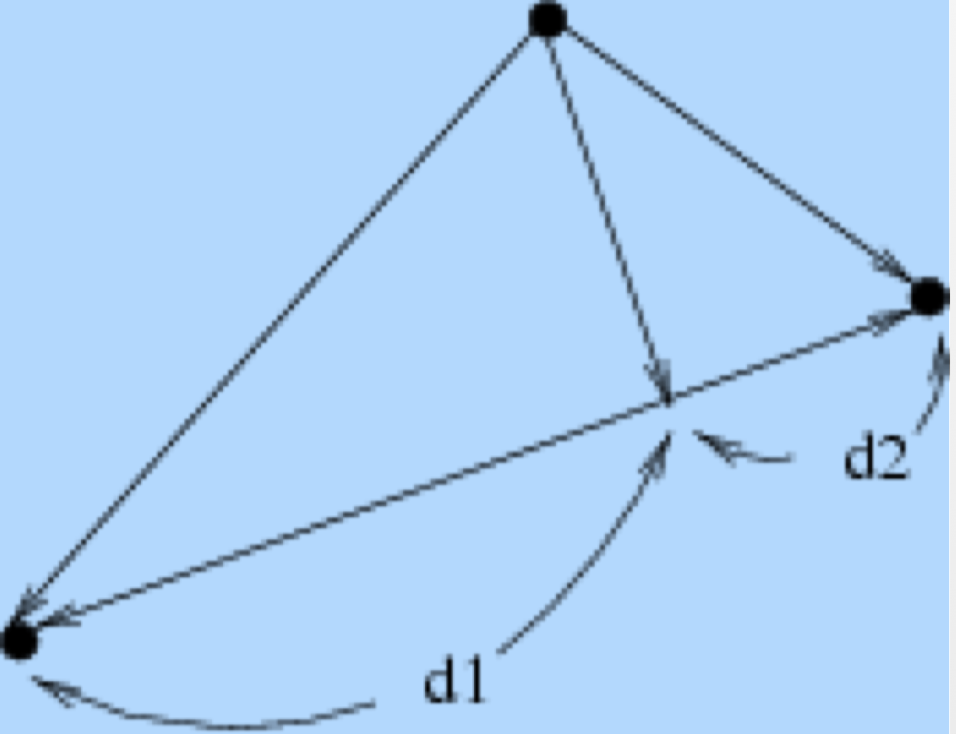
\includegraphics[scale=0.4]{img/proj}
\caption{...}
\label{proj}
\end{figure}

If $K>3$ we can look for a $L<K-1$ dimensional subspace optimal for LDA. Fisher defined \textit{optimal} such that the projected centroids were spread out as much as possible in terms of variance.
This problem, finding the principal component subspaces of the centroids, involves the following steps:
\begin{itemize}
\item compute the $k\times p$ matrix of class centroids $M$ and the common covariance matrix $W$ for within-class covariance;
\item compute $M*=MW^{-\frac{1}{2}}$ using the eigen-value decomposition;
\item compute $B*$, the covariance matrix of $M*$ ($B$ for between class covariance) and its eigenvalue decomposition $B^{*}=V^{*}D_BV^{*T}$. The columns $v^*_\ell$ from the first to the last define the coordinates of optimal subspaces.
\end{itemize}
The $lth$ discriminant variable is given by $Z_\ell =  v_\ell^TX$ with $v_\ell=W^{-\frac{1}{2}} v^*_\ell$.  Although the direction joining the centroids separates the means as much as possible(maximizes the between class covariance), there is an overlap between the projected classes due to the nature of covariances. Taking the covariances into account reduce the overlap and that is what we are doing (\autoref{cov}).

\begin{figure}
\centering
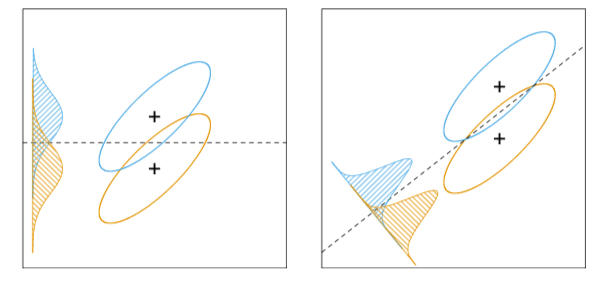
\includegraphics[scale=0.4]{img/cov}
\caption{Covariance.}
\label{cov}
\end{figure}

The between-class variance $Z$ is $a^TBa$ and the within class variance is $a^TWa$, with $B+W=T$, the total covariance matrix of $X$.
Fisher's problem maximizes the \textit{Rayleigh quotient}:

\begin{equation}
max_{a} \frac{a^TBa}{a^TWa}
\end{equation}

This is a generalized eigenvalue problem, with $a$ given by the largest eigenvalue. Similarly one can find the next direction $a_2$, orthogonal in $W$ to $a_1$, such that $a^T_2 Ba_2/a^T_2 Wa_2$ is maximized; the solution is a$_2 = v_2$, and so on. $a_\ell$ are the \textit{discriminant coordinates} or \textit{canonical variates}, different from discriminant functions.

The reduced subspaces can be used both for visualization and classification by limiting the distance between centroids to the chosen subspace. However, when doing this, due to the Gaussian classification, a correction factor of $\log \pi_k$ is needed. The misclassification is given by the overlapping area in \autoref{cov} between the two densities. When both classes have the same priors $\pi_k$ as in the figure, the optimal cut-point is the midway between projected means, if not the cut-point is moved towards the smaller class to have a better error rate.

For $2$ classes one can derive the linear rule using LDA, and then choosing the cut-point to minimize misclassification error.

\subsection{Logistic regression}
\label{LogReg}
The idea behind logistic regression is to still exploit a linear model $x^T\beta$ but having its output representing a probability, i.e., constrained between $0$ and $1$. This part is performed using the \tb{sigmoid function}:

\begin{equation}
p=\sigma(q) = \frac{1}{1+e^{-q}}.
\end{equation}
Inverting the terms we get 
\begin{equation}
\label{logit}
q = -\log\frac{1-p}{p} = \log \frac{p}{1-p} 
\end{equation}
\autoref{logit} is called \textbf{logit function}. As $q$ increases to $\infty$, the output of the sigmoid gets closer to $1$; instead when it diverges to $-\infty$ we get $0$. Suppose we have just 2 classes or equivalently a binary classifier that tells the probability of an event to happen: $Y_n=1$ when the event happens and $Y_n=0$ when it does not. We can express the probabilities output by our classifier when new input data $x_{new}$ are observed as:
\begin{equation}
\begin{aligned}
&P(G=1|x_n, \beta) =  \frac{1}{1+e^{-\beta^T\x_{new}}}\\
&P(G=0|x_n, \beta) = 1- \frac{1}{1+e^{-\beta^T\x_{new}}} = \frac{e^{-\beta^T\x_{new}}}{1+e^{-\beta^T\x_{new}}}
\end{aligned}
\end{equation}

These equations can be combined in a single equation:
\begin{equation}
P(G=g|x_n, \beta) =  P(G=1|x_n, \beta)^{g} P(G=0|x_n, \beta)^{g-1}
\end{equation}

Taking the log-ratio between the two probabilities we have:
\begin{equation}
\begin{aligned}
\log \frac{P(Y_n=0|x_n, \beta)}{P(Y_n=1|x_n, \beta)} =  \log \frac{\frac{e^{-\beta^T\x_{new}}}{\cancel{1+e^{-\beta^T\x_{new}}}}}{\frac{1}{\cancel{1+e^{-\beta^T\x_{new}}}}} = -\beta^T\x_{new}
\end{aligned}
\end{equation}
So we are using lines (or hyperplanes) to separate the two classes.

\subsubsection{Multinomial logistic regression: more than 2 classes}
Now suppose we have more than two classes and we still want to separate those classes with linear functions, which means we will have a hyperplane separating two classes. We have $K$ possible outcomes. We can think to run $K-1$ independent binary logistic regressions with one class chosen as \textbf{pivot}, generally the one corresponding to class $K$, and with the other $K-1$ classes separately regressed against the pivot:
%LR models the posterior probabilities of the classes as linear function in $x$, while ensuring they sum up to $1$.
%The model has the form
\begin{equation}
\begin{aligned}
&\log \frac{Pr\left(G=1|X=x\right)}{Pr\left(G=K|X=x\right)} = \beta_1^T x \\
&\log \frac{Pr\left(G=2|X=x\right)}{Pr\left(G=K|X=x\right)} = \beta_2^T x\\
\vdots\\
&\log \frac{Pr\left(G=K-1|X=x\right)}{Pr\left(G=K|X=x\right)} = \beta_{\left(K-1\right)}^T x
\end{aligned}
\label{logratio}
\end{equation}
The choice of the pivot class used as denominator is arbitrarily and the estimates are equivalent under different choices.

Summing the probability of each class we must get $1$:
\begin{equation}
\begin{aligned}
&\sum_{\ell=1}^{K} Pr\left(G=\ell|X=x\right) = 1 \Rightarrow Pr\left(G=K|X=x\right)+ \sum_{\ell=1}^{K-1} Pr\left(G=\ell|X=x\right)=1\\
&\Rightarrow Pr\left(G=K|X=x\right) +\sum_{\ell=1}^{K-1} Pr\left(G=K|X=x\right)e^{\beta_\ell^Tx}=1\\
&\Rightarrow Pr\left(G=K|X=x\right) \br{1+\sum_{\ell=1}^{K-1} e^{\beta_\ell^Tx}}=1\\
&\Rightarrow Pr\left(G=K|X=x\right)= \frac{1}{1+\sum_{\ell=1}^{K-1} e^{\beta_\ell^Tx}}
\end{aligned}
\end{equation}
where the \autoref{logratio} has been substituted in.
So we can re-express the probabilities as:

\begin{equation}
Pr\left(G=k|X=x\right) = \frac{e^{\beta_{k}^T x}}{1+\sum_{\ell=1}^{K-1} e^{\beta_\ell^Tx}}
\end{equation}

Note that the boundaries between any two classes are linear:
\begin{equation*}
\log \frac{Pr(G=i|X=x)}{Pr(G=j|X=x)} = \log \frac{e^{\beta_i^T x}}{e^{\beta_j^T x}} = \br{\beta_i -\beta_j}x
\end{equation*}

\subsubsection{Another approach: the softmax function}
\label{sssec:softmax}
As already stated we want linear boundaries between classes. This means that for any pair of classes:
\begin{equation}
\log \frac{Pr\left(G=i|X=x\right)}{Pr\left(G=j|X=x\right)} = (\beta_i - \be_j)^T x 
\end{equation}
or equivalently:
\begin{equation}
Pr\left(G=i|X=x\right) = \frac{1}{C}e^{\beta_i ^T x }
\end{equation}
Forcing the sum of all probabilities to be $1$, one gets:
\begin{equation}
C= \frac{1}{\sum_{j=1}^Ke^{\beta_j ^T x }}
\end{equation}
So:
\begin{equation}
Pr\left(G=i|X=x\right) = \frac{1}{\sum_{j=1}^Ke^{\beta_j ^T x}}e^{\beta_i ^T x }
\label{eq:softmax}
\end{equation}
\autoref{eq:softmax} is called \tb{Softmax function}. 
The softmax function is a redundant function. Suppose one subtracts a constant quantity from each of the parameter: $\beta_i \rightarrow \beta_i - p$:
\begin{equation}
\begin{aligned}
Pr\left(G=i|X=x\right) &= \frac{1}{\sum_{j=1}^Ke^{(\beta_j-p) ^T x}}e^{(\beta_i-p)  ^T x } =\\
&= \frac{1}{\sum_{j=1}^Ke^{(\beta_j) ^T x}\cancel{e^{-px}}}e^{(\beta_i)  ^T x }\cancel{e^{-px}}
\end{aligned}
\end{equation}
In other words, subtracting $p$ from parameter does not affect our hypothesis'predictions at all. This shows that softmax regression's parameters are "redundant". More formally, we say that our softmax model is \tb{overparameterized}, meaning that for any hypothesis we might fit to the data, there are multiple parameter settings that give rise to exactly the same model mapping from inputs $x$ to the predictions.

Furthermore, the set of parameters that minimise a cost function is not unique, even if the cost function is convex and has a global minimum, and thus gradient descent will not run into local optima problems (but the Hessian is singular/non-invertible, which causes a straightforward implementation of Newton’s method to run into numerical problems \footnote{\url{http://deeplearning.stanford.edu/tutorial/supervised/SoftmaxRegression/}}).

One way to eliminate such redundancy, is to specify a further condition: suppose $\beta_K = 0$, then one gets:
\begin{equation}
Pr\left(G=i|X=x\right) = \frac{1}{1+\sum_{j=1}^{K-1} e^{\beta_j ^T x}}e^{\beta_i ^T x }
\end{equation}
which is the form of the classifier seen in the previous chapter.

\paragraph{\tb{Monotonicity of the softmax function}} The softmax function is monotonic, i.e., when the exponent $\be_i^T x$) increases, the probability of the class $i$ increases while, the ones of the other classes decrease. Intuitively this is due to the fact that the sum must be always $1$.
\begin{proof}
Suppose that for a given input $x$ we want to increase $Pr(G=i)$. To do that one has to increase the numerator which in turns means to increase the exponent $\be_i x$. Let us call $\be_i x = a_i$, the quantity to be increased in order to have a higher probability of that class. Let us take the derivative with respect to $a_i$:
\begin{equation}
\begin{aligned}
\frac{\partial softmax}{\pr a_i} &=\frac{\partial }{\pr a_i}  \br{\frac{1}{\sum_{j=1}^Ke^{a_j}}e^{a_i} } =\frac{e^{a_i} \sum_{j=1}^Ke^{a_j} - e^{a_i} e^{a_i} } {\br{\sum_{j=1}^Ke^{a_j}}^2} = \\
&=\frac{e^{a_i} \sum_{j=1\setminus i}^Ke^{a_j} }{\br{\sum_{j=1}^Ke^{a_j}}^2} \\
\end{aligned}
\end{equation}
The quantities at the numerator and denominator are all positive, i.e., the partial derivative is positive and so the softmax function is increasing the value $Pr(G=i)$.

Now let us take the derivative with respect to $a_j$:
\begin{equation}
\begin{aligned}
\frac{\partial softmax}{\pr a_j} &=\frac{\partial }{\pr a_j}  \br{\frac{1}{\sum_{j=1}^Ke^{a_j}}e^{a_i} }=\frac{-e^{a_j} e^{a_i} } {\br{\sum_{j=1}^Ke^{a_j}}^2}
\end{aligned}
\end{equation}
which is obviously a negative quantity. Hence when the quantity $a_j$ of another class is increased, the other classes will have a reduced probability.
\end{proof}

\paragraph{\tb{Why the is it called \tb{softmax function?}}}Consider a slightly modified version of the softmax: 

$$\frac{e^{c\cdot z_j}}{\sum_k e^{c\cdot z_k}}$$

With $c=1$ we get back to the softmax.

This is for sure still a probability distribution: everything sums up to $1$, and all quantities are positive. So we can write for the event $j$:

$$P(j) = \frac{e^{c\cdot z_j}}{\sum_k e^{c\cdot z_k}}$$

Now take the limit $c\rightarrow\infty$.

Consider the ratio of two probabilities and takes to limit to infinity:

$$\lim_{c\rightarrow \infty}\frac{e^{c\cdot z_j}}{e^{c\cdot z_k}} = \lim_{c\rightarrow \infty} e^{p(z_j-z_k)}$$

It can be $1$ if $z_j=z_k$, $0$ if $z_j<z_k$, or $\infty$ otherwise.

Now consider the second case. For each $j$ for which this happens, it means that at the denominator of $P(j)$ there is a quantity that goes to infinity faster (or to $0$ slower) than the denominator. Then $P(j)=0$.

So the only $P$ different from zero are the one(s) equal to the biggest value. Suppose there are $n$ such elements for which this hold, i.e., $n$ elements for which $z_\ell=z_m$ (I used different indexes to avoid confusion).

Then:

$$\lim_{c\rightarrow \infty} P(\ell) = \frac{e^{c\cdot z_\ell}}{n e^{c\cdot z_\ell}}  = \frac{1}{n}$$

If you put these elements in a vector you get a vector of zeros, except for those elements for which the value is maximum. In classification problems, where softmax is used, typically there is one element having the maximum value (its probability is bigger than the others). So the resulting vector is a vector of one element of $1$ and all the others of $0$. Anyway such a vector has values different from zero for those elements having a maximum value: it is basically the a function that maximise the maximum value(s): having probabilities, the biggest possible value is $1$. This is commonly termed \tb{max function}. 

In the softmax one takes $c=1$, it is like taking a soften version of the above function: it is a \tb{softmax}.

\subsubsection{Fitting logistic regression}
From now on we will consider a logistic regression for just two classes. 

As seen in \autoref{ClassBayes}, we want to find the best parameters for the chosen model according to some criteria. First let us apply the Bayes theorem:
\begin{equation}
Pr\left(\be|\y,\X,M\right) = \frac{Pr\left(\y|\be,\X,M\right) Pr(\be,M)}{Pr(\y|\X,M)}
\end{equation}
\textbf{From now on we will not write the conditional on the model for seek of brevity but we know it exists}.

This formula tells we want to find the coefficients given some input and output data. Let us analyse each term:
\begin{itemize}
\item $Pr(\be)$ (\textbf{prior distribution}): this is the prior belief about the parameters without seeing the data. As prior, we will use a Gaussian distribution with $0$ mean:  $\CMcal{N}(0, \sigma^2\I)$. In this way the parameters will depend on $\sigma^2$: more formally we should write $Pr(\be|\sigma)$ but we will skip. Although the choice of the Gaussian distribution with $0$ mean is analytically convenient as seen in \autoref{conjugacy}, we will not rely on conjugacy.
\item $Pr\left(\y|\be,\X\right)$ (\textbf{likelihood}): we will assume $y$ are conditionally independent (\autoref{dataset likelihood}):
\begin{equation}
Pr(\y|\X, \be) = \prod_{n=1}^N Pr(y_n|\x_n, \be)
\end{equation}
Since in this case we have a binary variable, instead of a Gaussian random variable, suitable for real values distribution, we will consider a binary random variable $Y_n$ characterised by the probability of the second class:
\begin{equation}
Pr(\y|\X, \be) = \prod_{n=1}^N Pr(Y_n=y_n|\x_n, \be)
\end{equation}
\item $Pr(\y|\X)$(\textbf{marginal likelihood}): It can be expressed as 
\begin{equation}
Pr(\y|\X) = \int Pr\left(\y|\be,\X\right) Pr(\be) d\be
\end{equation}
\end{itemize}

So the numerator can be calculated and results in a Gaussian function not in standard form (\autoref{gaussian}). The denominator, or marginal likelihood, as we have seen can be expressed as $Pr(\y|\X) = \int Pr\left(\y|\be,\X\right) Pr(\be) d\be$. Mathematically this integral has no close solution since (again see \autoref{gaussian}) and the impossibility of the integral of $e^{-x^2})$, unless an ad-hoc prior distribution is chosen.

When we cannot directly compute the posterior density (due to the denominator), we have three options:
\begin{enumerate}
\item find the single value $\be$ that corresponds to the highest value of the posterior. This is equivalent to find the value $\be$ that maximize the numerator since the denominator is not a function of $\be$ but a numerical value.
\item Approximate $Pr(\be|\X, \y)$ with some other density that we can compute analytically.
\item Sample directly from the posterior $Pr(\be|\X,\y)$ knowing only the numerator.
\end{enumerate}

The first method is simple and hence popular but it is not very "Bayesian", since we will make predictions of new data based on a single value and not a distribution. The whole Bayesian theory is based on making an hypothesis and getting feedback from the data that can validate or not that hypothesis. Also when using a distribution we get also measures on how confident we are about the estimated model. For example when estimating a Gaussian distribution, we estimate the coefficients $\mu$ and $\sigma^2$: the smallest the latter value the more confident we are about the model. When using a single value we loose this piece of information.

With the second method we get a density easy to work with but if the chosen density is very different from the posterior our model will not be very reliable.

The third method samples from the posterior and hence to get a good approximation but it can be difficult.

\subsubsection{First method: point estimation, the MAP solution}
We have seen that in some cases we cannot compute the posterior but we can compute the numerator of the expression, i.e., the prior multiplied by the likelihood. The value that maximizes the posterior is also the value that maximizes the numerator. We have already seen a likelihood maximization procedure in \autoref{likelihoodMax}; here we are maximizing the likelihood times the prior. This solution is the \textbf{maximum a posteriori (MAP)} estimate.

\paragraph{The Newton-Raphson method}
\label{NewtonsMethod}
The Newton-Raphson method finds the points where $f(x)=0$. Starting from an estimation $x_n$ of such points, the estimation is updated by moving to the point where the tangent to the function at $x_n$ passes throw the x-axis. This point is computed by approximating the gradient as a change in $f(x)$ divided by a change in $x$:

\begin{figure}
\centering
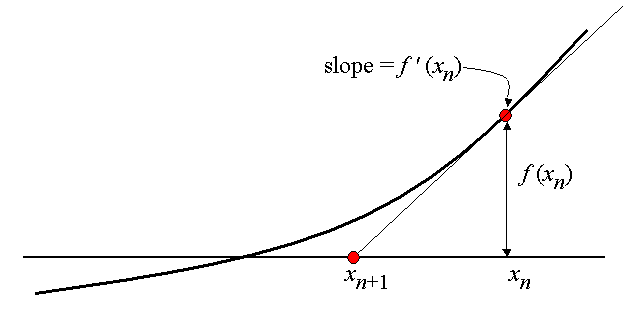
\includegraphics[scale=0.3]{img/NewtonRaphson}
\caption{Newton-Raphsone example.}
\end{figure}

\begin{equation}
\begin{aligned}
f'(x_n) = -\frac{f(x_n)-0}{x_n -x_{n+1}}\\
\Rightarrow x_{n+1} = x_n -\frac{f(x_n)}{f'(x_n)}
\end{aligned}
\end{equation}
Instead of finding the point for which $f(x)=0$, we want to find the point where its derivative is $0$. Hence we substitute $f(x)$ with $f'(x)$ and $f'(x)$ with $f''(x)$. In this way the method can be used to find points where the gradient passes through $0$, i.e., minima, maxima and points of inflections:
\begin{equation}
\begin{aligned}
f''(x_n) = -\frac{f'(x_n)-0}{x_n -x_{n+1}}\\
\Rightarrow x_{n+1} = x_n -\frac{f'(x_n)}{f''(x_n)}
\end{aligned}
\end{equation}
When dealing with vectors, $f'(x)$ is replaced by the vector of partial derivatives evaluated at $x_n$ and $\frac{1}{f''(x_n)}$ is replaced by the inverse of the Hessian matrix $\frac{-\partial^2 f(x)}{\partial \x \partial \x^T}$.

\paragraph{Derivation}
As already done, instead of maximizing the function itself, we maximize its logarithmic. Apart from the mathematical convenience this is also the advantage of avoiding underflow: we are dealing with probabilities, numbers between $0$ and $1$ and these might be too small to have a sufficient numerical precision. As the numbers go to $0$,the logarithmic makes the number goes to infinity, guaranteeing a better numerical precision.
 Since we cannot compute the derivative and set it to $0$, we use the Newton-Raphson procedure. Let us call the numerator $g(\be,\X,\y) = Pr(\y|\be,\X)Pr(\be|\X)$:

\begin{equation}
\be' = \be - \br{\frac{\partial^2\log g(\be,\X,\y)}{\partial \be \partial \be^T}}^{-1} \frac{\partial \log g(\be,\X,\y)}{\partial \be}
\end{equation}

The procedure is iterative and stops when the gradient is $0$. To check the point we have converged to corresponds to a minimum we check the Hessian matrix is negative definite.

Before computing the derivatives we re-express $g(\be,\X,\y)$.

\begin{equation}
\begin{aligned}
&\log g(\be,\X,\y) = \sum_{n=1}^N \log Pr(Y_n=y_n|\x_n, \be) + \log Pr(\be|\sigma^2) = \\
&=  \sum_{n=1}^N \log \left[\br{\frac{1}{1+e^{-\be^T\x_n}}}^{y_n} \br{\frac{e^{-\be^T\x_n}}{1+e^{-\be^T\x_n}}}^{1-y_n}\right] + \log Pr(\be|\sigma^2) =
\end{aligned}
\end{equation}
We denote $P_n=P(Y_n=1|\be, \x_n) = \frac{1}{1+e^{-\be^T\x_n}}$:
\begin{equation}
\begin{aligned}
&\log g(\be,\X,\y) =  \sum_{n=1}^N \log P_n^{y_n} +\log(1-P_n)^{1-y_n}+ \log Pr(\be|\sigma^2) =
\end{aligned}
\end{equation}
Racalling
\begin{equation}
\begin{aligned}
Pr(\be|\sigma^2)  =& \frac{1}{\sqrt{(2\pi)^D|\Sigma|}} e^{-\frac{\br{\be-\cancel{\mu}}^T\br{\be-\cancel{\mu}}}{2\sigma2}}\\
\Rightarrow\log g(\be,\X,\y) =&  \sum_{n=1}^N \log P_n^{y_n} +\log(1-P_n)^{1-y_n} -\frac{D}{2}\log(2\pi) - D\log\sigma +\\
&- \frac{1}{2\sigma^2} \be^T\be
\end{aligned}
\end{equation}

Now we can take the derivative:
\begin{equation}
\label{devg}
\begin{aligned}
&\frac{\partial \log g(\be,\X,\y)}{\partial \be} = - \frac{1}{\sigma^2} \be + \sum_{n=1}^N \frac{y_n}{P_n}\frac{\partial P_n}{\partial \be} + \frac{1-y_n}{1-P_n}\frac{\partial (1-P_n)}{\partial \be} =\\
&=\frac{\partial \log g(\be,\X,\y)}{\partial \be} = - \frac{1}{\sigma^2} \be + \sum_{n=1}^N \frac{y_n}{P_n}\frac{\partial P_n}{\partial \be} - \frac{1-y_n}{1-P_n}\frac{\partial P_n}{\partial \be}
\end{aligned}
\end{equation}

Now we must calculate $\frac{\partial P_n}{\partial \be}$:
\begin{equation}
\label{devPn}
\begin{aligned}
\frac{\partial P_n}{\partial \be} =& \frac{\partial}{\partial \be} \frac{1}{1+e^{-\be^T\x_n}} = \frac{\partial}{\partial \be} \br{1+e^{-\be^T\x_n}}^{-1} =\\
=& \frac{1}{\br{1+e^{-\be^T\x_n}}^2}  \frac{\partial}{\partial \be} \br{1+e^{-\be^T\x_n}} = \\
=&  -\x_n \frac{e^{-\be^T\x_n}}{\br{1+e^{-\be^T\x_n}}^2}   = -x_n \frac{1}{\br{1+e^{-\be^T\x_n}}}\frac{e^{-\be^T\x_n}}{\br{1+e^{-\be^T\x_n}}} =\\
=& -\x_nP_n \br{1-P_n}
\end{aligned}
\end{equation}
Substituting in \autoref{devg}:
\begin{equation}
\begin{aligned}
\frac{\partial \log g(\be,\X,\y)}{\partial \be} =&  - \frac{1}{\sigma^2} \be + \sum_{n=1}^N \frac{y_n}{P_n}\frac{\partial P_n}{\partial \be} - \frac{1-y_n}{1-P_n}\frac{\partial P_n}{\partial \be} =\\
=&- \frac{1}{\sigma^2} \be + \sum_{n=1}^N \frac{y_n}{P_n}\left[-\x_nP_n \br{1-P_n}\right]+ \\
&\quad  - \frac{1-y_n}{1-P_n}\left[-\x_nP_n \br{1-P_n}\right] =\\
=& - \frac{1}{\sigma^2} \be + \sum_{n=1}^N -y_n\x_n \br{1-P_n} - (1-y_n)(-\x_nP_n ) = \\
=& - \frac{1}{\sigma^2} \be + \sum_{n=1}^N \x_n (y_n-P_n)
\end{aligned}
\end{equation}

Now we must compute the Hessian matrix:
\begin{equation}
\begin{aligned}
&\frac{\partial^2 \log g(\be,\X,\y)}{\partial \be \partial\be^T}  = \frac{\partial}{\partial \be^T} \br{- \frac{1}{\sigma^2} \be + \sum_{n=1}^N \x_n (y_n-P_n)} =
\\ &=- \frac{1}{\sigma^2} \I -\sum_{n=1}^N \x_n \frac{\partial P_n}{\partial \be^T} = - \frac{1}{\sigma^2} \I - \sum_{n=1}^N \x_n \x_n^TP_n \br{1-P_n}
\end{aligned}
\end{equation}
where we used the result from \autoref{devPn}.

Note that the 2 terms are negative definite, hence the Hessian is always negative definite. Therefore there can only be one optimum and it must be the minimum.

The decision boundary is the one for which $Pr(Y_n=1|\x,\hat{\be}=0.5)$.

The steps above can be done for any prior and likelihood combination. In some cases the posterior might have several maxima and or some minima and it become difficult to know if the maximum is a global optimum.


The \textit{Elements of Statistical Learning} book instead of maximizing posterior (or equivalently the numerator), it maximizes the likelihood.
Let us express $Pr\left(G=k|X=x\right)=p_k(x,\theta)$ with $\theta = \left\lbrace \beta_{10},\beta_1^T,\cdots, \beta_{\left(K-1\right)0},\beta_{K-1}^T\right\rbrace$
and let us define the log-likelihood
\begin{equation}
\ell(\theta) = \sum_{i=1}^N \log p_{g_i}\left(x_i, \theta\right)
\end{equation}

Consider just two classes with responses $0$, $1$ and let $p_1(x,\theta) =p(x,\theta) $ and $p_2(x,\theta) =1-p(x,\theta)$. Recall that having two classes $\sum_{\ell=1}^{K-1} e^{\beta_{l0}+\beta_\ell^Tx_i} = e^{\beta_{10}+\beta_1^Tx_i}$. The log-likelihood can be written as:
\begin{equation}
\begin{aligned}
&\ell(\beta) = \sum_{i=1}^N \left\lbrace y_i \log p\left(x_i,\beta\right) + \left(1-y_i\right) \log \left(1-p\left(x_i,\beta\right)\right)\right\rbrace =\\
&=\sum_{i=1}^N y_i \log \frac{e^{\beta_{10} +\beta_{1}^T x_i}}{1+\sum_{\ell=1}^{K-1} e^{\beta_{l0}+\beta_\ell^Tx_i}}  +\\
& \quad\quad + \sum_{i=1}^N \left(1-y_i\right) \log \left(1-\frac{e^{\beta_{10} +\beta_{1}^T x_i}}{1+\sum_{\ell=1}^{K-1} e^{\beta_{l0}+\beta_\ell^Tx_i}}\right)= \\
&= \sum_{i=1}^N  y_i \log \frac{e^{\beta_{10} +\beta_{1}^T x_i}}{1+e^{\beta_{10}+\beta_1^Tx_i}} + \\
&\quad\quad +\sum_{i=1}^N  \left(1-y_i\right) \log \left(1-\frac{e^{\beta_{10} +\beta_{1}^T x_i}}{1+e^{\beta_{10}+\beta_1^Tx_i}}\right) = \\
&=\sum_{i=1}^N y_i \left(\log e^{\beta_{10} +\beta_{1}^T x_i} -\log \left(1+ e^{\beta_{10}+\beta_1^Tx_i}\right) \right) + \\
& \quad\quad + \sum_{i=1}^N  \left(1-y_i\right) \log \frac{1}{1+ e^{\beta_{10}+\beta_1^Tx_i}} = \\
&=\sum_{i=1}^N y_i \left(\log e^{\beta_{10} +\beta_{1}^T x_i} -\log \left(1+ e^{\beta_{10}+\beta_1^Tx_i}\right) \right) + \\
& \quad\quad - \sum_{i=1}^N\left(1-y_i\right) \log \left(1+ e^{\beta_{10}+\beta_1^Tx_i}\right) = \\
&=\sum_{i=1}^N \left\lbrace y_i \left(\beta_{10} +\beta_{1}^T x_i \right) -log \left(1+ e^{\beta_{10}+\beta_1^Tx_i}\right) \right\rbrace
\end{aligned}
\end{equation}
Here $\beta = \left[ \beta_{10}, \beta_1\right]$. To maximize the log-likelihood we set the derivative to $0$:
\begin{equation}
\frac{\partial \ell(\beta)}{\partial \beta} = \sum_{i=1}^N x_i  (y_i - p(x_i, \beta) = 0
\end{equation}

Using the \textit{Newton-Raphson} algorithm that requires the second-derivative:
\begin{align}
&\frac{\partial^2 \ell(\beta)}{\partial \beta \partial \beta^T} = -\sum_{i=1}^N x_ix_i^T   p(x_i, \beta) (1-p(x_i, \beta)\\
&\Rightarrow \beta^{new} = \beta^{old} - \left( \frac{\partial^2 \ell\left( \beta\right) }{\partial \beta \partial \beta^T} \right)^{-1}\frac{\partial \ell(\beta)}{\partial \beta}
\end{align}
Using the matrix notation,
\begin{align}
\frac{\partial \ell(\beta)}{\partial \beta} =  X^T (y-p) \\
\frac{\partial^2 \ell(\beta)}{\partial \beta \partial \beta^T} = -X^TWX
\end{align}
So the Newton step becomes

\begin{equation}
\begin{aligned}
&\beta^{new} = \beta^{old} +(X^TWX)^{-1}X^T(y-p) = \\
&=(X^TWX)^{-1}X^TW\left(X\beta^{old}+W^{-1} \left(y-p\right)\right) =\\
&= \left(X^TWX\right)^{-1} X^TWz
\end{aligned}
\end{equation}
with
\begin{equation}
z = X\beta^{old}+ W^{-1} (y-p)
\end{equation}
sometimes known as the adjusted response. This algorithm is known as \textbf{iteratively reweighted least squares (IRLS)} since each iteration solves the weighted least square problem:
\begin{equation}
\beta^{new} \leftarrow \argmin{\beta}{\left(z-X\beta\right)^TW\left(z-X\beta\right)}
\end{equation}
$\beta=0$ seems a good starting value. Convergence is never guaranteed but typically the algorithm does converge, since the log-likelihood is concave but overshooting can occur. In the rare cases that the log-likelihood decreases, step size halving will guarantee convergence.

For $K>2$ we still use the iteration procedure but we will have a $K-1$ vector response and a non-diagonal weight matrix per observation. In this case it is better to work with the vector $\theta$ directly.

\subsubsection{Second method: Laplace approximation}
There are many approximation methods but the most common is the Laplace approximation. The idea is to approximate the density of interest with a Gaussian.

Choosing a Gaussian means choosing a proper variance and mean value. The Laplace approximation method fixes one of the two parameters, i.e., the mean to the value maximizing the posterior, $\beta$. We approximate $\log g(\be,\X,\y)$ with the Taylor expansion around $\hat{\be}$:
\begin{equation}
\label{Taylor}
\begin{aligned}
\log g(\be,\X,\y) \approx &\log g(\hbe,\X,\y) + \cancel{\frac{ \partial \log g(\be,\X,\y)}{\partial \be}\bigg\rvert_{\hbe}\br{\be -\hbe}} + \\
&+ \frac{ \partial^2 \log g(\be,\X,\y)}{\partial \be^2}\bigg\rvert_{\hbe}\br{\be -\hbe}^2 =\\
&=\log g(\hbe,\X,\y)+ \frac{ \partial^2 \log g(\be,\X,\y)}{\partial \be^2}\bigg\rvert_{\hbe}\frac{\br{\be -\hbe}^2}{2}
\end{aligned}
\end{equation}

where the second term is the gradient evaluated at the maximum point that therefore must be $0$.

The Gaussian density and its log are the following:
\begin{equation}
\begin{aligned}
&\frac{1}{2\pi}e^{-\frac{(\be-\hbe)^2}{2\sigma^2}}\\
\Rightarrow &\log const -\frac{1}{2\sigma^2}\br{\be-\mu}^2
\end{aligned}
\end{equation}
which is similar to \autoref{Taylor}. By analogy of the two equations:
\begin{equation}
\begin{aligned}
&\mathbf{\mu} = \hbe\\
&-\frac{1}{\sigma^2} = -\frac{ \partial^2 \log g(\be,\X,\y)}{\partial \be^2}\bigg\rvert_{\hbe}
\end{aligned}
\end{equation}

It can be applied also to multivariate densities  $Pr(\be,\X,\y) \approx \CMcal{N}(\mathbf{\mu, \Sigma})$:
\begin{equation}
\begin{aligned}
&\mathbf{\mu} = \hbe\\
&\Sigma^{-1} = -\frac{ \partial^2 \log g(\be,\X,\y)}{\partial \be\partial\be^T}\bigg\rvert_{\hbe}
\end{aligned}
\end{equation}

Consider a multinomial 2D Gaussian function (dimensionaity of $\be$ is 2) as in \autoref{gaussianfig} and suppose to project on the plane the points of the curve having the same value (the ellipses in the figure). The ellipses will be the combination of coefficients giving the same function value.
\begin{figure}
\centering
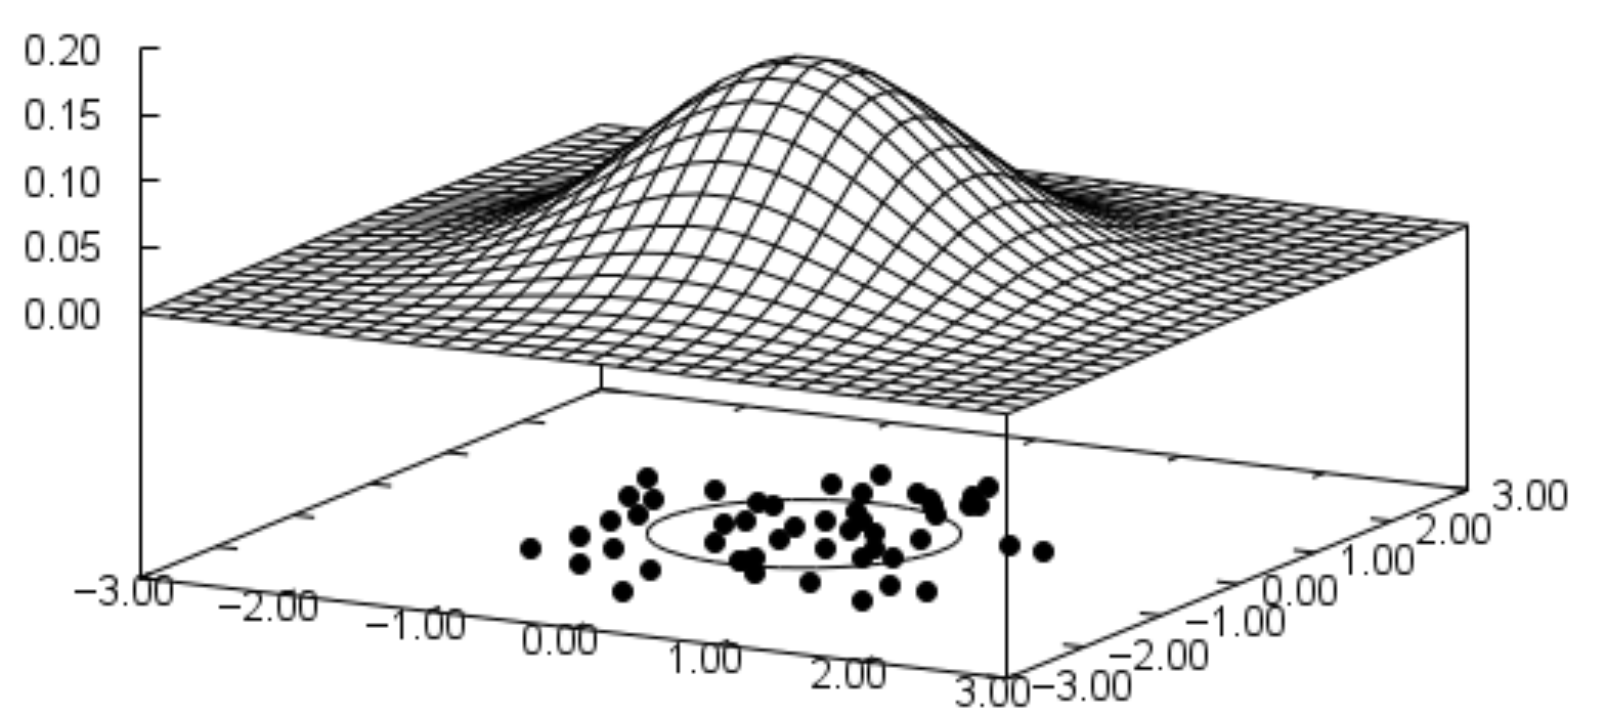
\includegraphics[scale=0.4]{img/gaussian}
\caption{Example of multinomial Gaussian.}
\label{gaussianfig}
\end{figure}

In figure \autoref{posteriorApprox} the Laplace approximation of the posterior (darker lines) is shown while the lighter lines are the true unnormalised posterior. The centre point corresponds to the maximum point $\hbe$. Note how the approximation is good around $\hbe$ and it diverges going further from it.
\begin{figure}
\centering
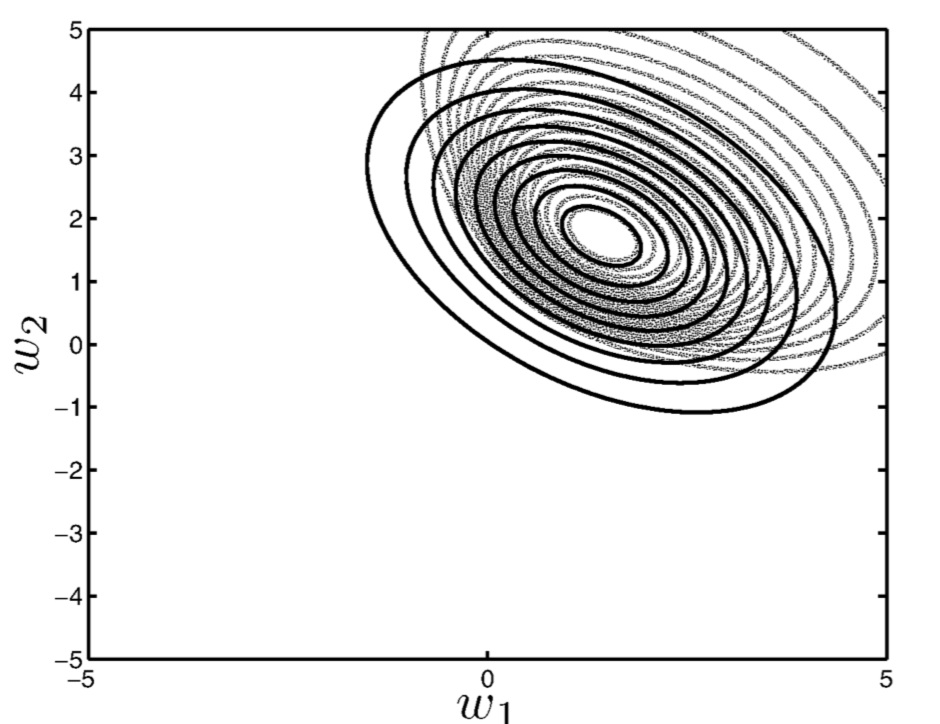
\includegraphics[scale=0.4]{img/posteriorApprox}
\caption{The axis are the parameters. The Laplace approximation of the posterior (darker lines) is shown while the lighter lines are the true unnormalised posterior. The centre point corresponds to the maximum point $\hbe$.}
\label{posteriorApprox}
\end{figure}

We use the approximate posterior to compute predictions. But now we have a density and not a single value: the prediction is computed by averaging over this density: it is like averaging over all possible values of $\be$. We should calculate the expected value $Pr(Y_{new} = 1|\x_{new}, \be)$ with respect to the approximate posterior denoted as $\CMcal{N}(\mathbf{\mu, \Sigma})$:
\begin{equation}
Pr(Y_{new}=1|\x_{new}, \X, \be) = \E_{\CMcal{N}(\mathbf{\mu, \Sigma})}\left\lbrace Pr(T_{new}=1| \x_{new}, \be)\right\rbrace
\end{equation}
However, we cannot compute the integral (of the expectation), but we can sample from $\CMcal{N}(\mathbf{\mu, \Sigma})$ and approximate the expectation with a sum:
\begin{equation}
\label{approxDen}
Pr(Y_{new}=1|\x_{new}, \X, \be) = \frac{1}{N_s}\sum_{s=1}^{N_s}\frac{1}{1+e^{-\be_s^T \x_{new}}}
\end{equation}

\paragraph{\textbf{Comparison between the decision boundaries of MAP and Laplace method.}} In case of MAP estimation we get a single separating line as in \autoref{MAP1} for the example of two classes. In case of Laplace approximation we don't have a single separating line but a density distribution. \autoref{laplace1} shows 20 boundaries (i.e., set of coefficients) sampled randomly from the distribution. All or almost all separates the classes quite well but in the area from the graph further from the classes (or from the centroids or clusters) there is a lot of variability. This variability represents the uncertainty of the classifier in those area far from the classes, where no event (in the sense of data entry) was observed.

This is made clearer by looking at the decision boundaries in \autoref{MAP2} and \autoref{laplace2}. In case of MAP it is quite obvious: the probability increases or decreases just moving close to or far from to the boundary. In case of Laplace approximation the contours are no longer straight lines. The probability are now close to $0.5$ in all the area except those closes to the two classes. It is like the classifier is unable to take a decision in those areas, that are the ones where no event has been noted.

On the contrary the classifier resulting from MAP approximation is always sure about its work: it can only classify either with one or the other class except in on the points on the boundaries. This result from the fact that it is the result of a single point and not a distribution: i.e., the amount of confidence on the result is left out.

\begin{figure}
\begin{subfigure}[t]{0.5\textwidth}
\centering
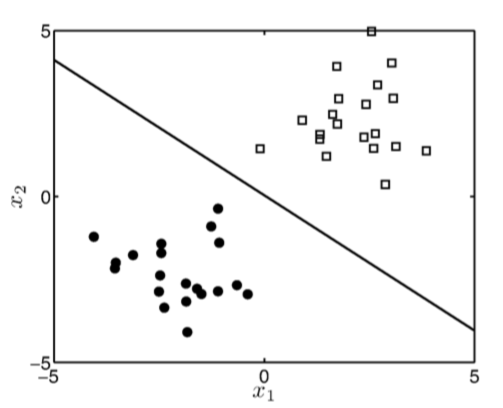
\includegraphics[width=0.85\linewidth]{img/MAP1}
\caption{Decision boundary for MAP estimation.}
\label{MAP1}
\end{subfigure}
\hfill
\begin{subfigure}[t]{0.505\textwidth}
\centering
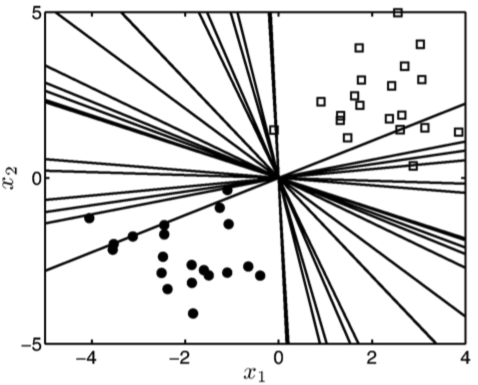
\includegraphics[width=0.8\linewidth]{img/laplace1}
\caption{Decision boundary for Laplace approximation estimation.}
\label{laplace1}
\end{subfigure}
\begin{subfigure}[t]{0.5\textwidth}
\centering
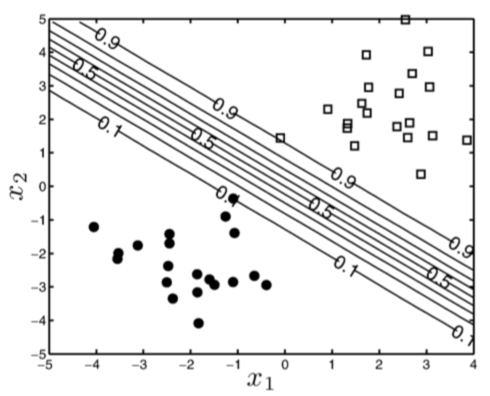
\includegraphics[width=0.8\linewidth]{img/MAP2}
\caption{Contours of probability of belonging to class 1 in case of MAP estimation.}
\label{MAP2}
\end{subfigure}
\hfill
\begin{subfigure}[t]{0.5\textwidth}
\centering
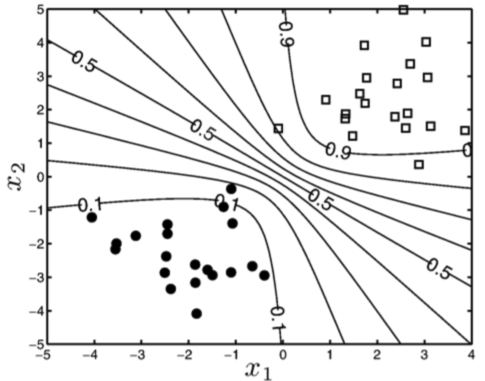
\includegraphics[width=0.8\linewidth]{img/laplace2}
\caption{Contours of probability of belonging to class 1 in case of Laplace approximation estimation computed with a sample based approximation.}
\label{laplace2}
\end{subfigure}
\caption{Comparison between MAP and Laplace approximation contours and probability densities.}
\end{figure}

\subsubsection{Third method: sampling technique	}
The reason of estimating the posterior density with Laplace approximation or any other method is to take into account uncertainties in $\be$ when making predictions. Using the Gaussian approximation we were able to sample as in equation \autoref{approxDen} directly from data. When deciding we take the conditional probability by averaging all over the potential values $\be$ by taking the expectation:
\begin{equation}
Pr(T_{new}=1| x_{new}, \X, \y, \sigma^2) = \E_{Pr(\be|\X, \y, \sigma^2)}\br{Pr(T_{new}=1|x_{new},\be}
\end{equation}

In these types of approximations we cut off the approximation step and sample directly from the posterior. A set of samples from the true posterior could be substituted directly into equation \autoref{approxDen} to compute the desired predictive probability $Pr(y_i|\x_i, \X, \be)$. A popular sampling technique is the \textbf{Metropolis-Hastings} algorithm.

Drawing from the posterior does not mean we can write it down but that we sample directly the system (physical or whatever) generating the data.

\paragraph{The metropolis-Hastings algorithms}
The objective is to sample from $Pr(\be|\X,\y,\sigma^2)$ to approximate the following expectation:
\begin{equation}
\begin{aligned}
Pr(Y_{new}&=1|x_{new},\X,\y,\sigma^2) = \E_{Pr(\be|\X,\y,\sigma^2)}\left[Pr(T_{new}=1|x_{new},\be) \right] \\
&=\int Pr(Y_{new}=1|x_{new},\be)Pr(\be|\X,\y,\sigma^2) d\be
\end{aligned}
\end{equation}
with 

\begin{equation}
\begin{aligned}
Pr(Y_{new}&=1|x_{new},\X,\y,\sigma^2) \approx \frac{1}{N_s}\sum_{s=1}^{N_s} Pr(Y_{new}=1|x_{new}, \be_s)
\end{aligned}
\end{equation}
The algorithm generates a sequence of samples $\be_1, \be_2, \cdots$. First all the algorithm is independent from the starting point, as long as we sample long enough: it is guaranteed the sequence converges.
\paragraph{\textbf{The generation of new samples}} happens in this way. Suppose we have the sample $s-1$, we will propose a new sample $\tilde{\be_s}$ and define the density $Pr(\tilde{\be}_s|\be_{s-1})$. This density is unrelated with the posterior $Pr(\be|\X,\y,\sigma^2)$ and we can define it as we please but it will affect the convergence time. A common choice is to use a Gaussian centred on the current sample, $\be_{s-1}$:
\begin{equation}
Pr(\tilde{\be}_s|\be_{s-1}, \Sigma) =\CMcal{N}(\be_{s-1}, \Sigma)
\end{equation}
Generally $\sigma$ is taken diagonal with same values. The smaller the elements on the diagonal, the smaller the distance at each step.

Such a sequence creates a \textbf{random walk}. The choice of the Gaussian is justified bye the easy of sampling from the Gaussian and by its symmetry: moving from $\tilde{\be}_{s-1}$ to $\tilde{\be}_s$ is just as likely to move from $\tilde{\be}_s$ to $\tilde{\be}_{s-1}$:
\begin{equation}
Pr(\tilde{\be}_s|\be_{s-1}, \Sigma)  = Pr(\tilde{\be}_{s-1}|\be_{s}, \Sigma) 
\end{equation}
\textbf{Accepting or rejecting the candidate $\tilde{\be}_s$} is performed by calculating the following quantity:
\begin{equation}
r = \frac{Pr(\tilde{\be}_s|\X, \y, \ssq)}{Pr(\be_{s-1}|\X, \y, \ssq)}\frac{Pr(\be_{s-1}|\tilde{\be}_s, \Sigma)}{Pr(\hat{\be}_{s}|\be_{s-1}, \Sigma)}
\end{equation}
The expression is the product of the ratio of the posterior density at the proposed sample to that at the old sample times the ratio of the proposed densities. For the Gaussian symmetry discussed above, this term is $1$ when using Gaussian densities. Note that we cannot compute exactly the densities, but being a ratio the normalisation constant (the denominator in Bayes expression) simplifies and only the likelihoods times the priors are left:
\begin{equation}
r = \frac{Pr(\tilde{\be}_s|\ssq)}{Pr(\be_{s-1}| \ssq)} \frac{Pr(\y|\X, \tilde{\be}_s, \ssq)}{Pr(\y|\X, \be_{s-1}, \ssq)}
\end{equation}
If $r>1$, i.e, we get a higher posterior density, we accept the candidate otherwise we accept the candidate with probability equal to $r$. The complete algorithm is depicted in \autoref{MHAlgo} where a uniform distribution in $[0,1]$ is used as decision rule in case $r<1$. Being a uniform distribution, the probability that $u \le r$ is $r$.

\begin{figure}
\centering
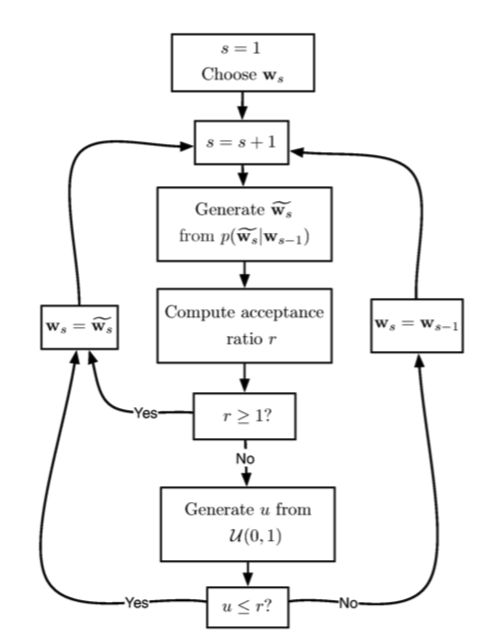
\includegraphics[scale=0.45]{img/MHAlgo}
\caption{The steps of the Metropolis-Hastings algorithm. $U$ is a uniform distribution in $[0,1]$}
\label{MHAlgo}
\end{figure}

\autoref{randomWalk} shows a 10-iteration process of the algorithms where solid lines are accepted coefficients, dashed lines are the rejected ones. Note that even the third sample causes a decrease in the posterior $r<1$, nevertheless in this specific case the decision rule accepted it. On the contrary the 4-th sample causes a huge decrease hence it is very unlikely it is accepted and in fact it is not, so $\be_4 = \be_3$. After $N$ samples we compute the sample based approximations to the mean and covariance
\begin{equation}
\begin{aligned}
\mu' &= \frac{1}{N_s} \sum_{s=1}^{N_s} \be_s\\
S' &= \frac{1}{N_s} \sum_{s=1}^{N_s} (\be_s-\mu')(\be_s-\mu')^T
\end{aligned}
\end{equation}

\begin{figure}
\centering
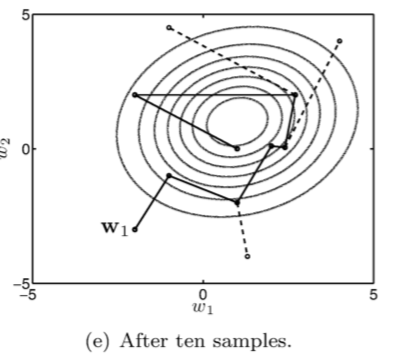
\includegraphics[scale=0.4]{img/randomWalk}
\caption{Example of Metropolis-Hastings iterations: solid lines are accepted coefficients, dashed lines are the rejected ones.}
\label{randomWalk}
\end{figure}

\begin{definition}{\textbf{Burn-in}} It is the time interval between the starting of the algorithm and the convergence. 
\end{definition}
It cannot be determined: to overcome this problem, a method for determining convergence (to a distribution, not to a value) should be established. For example, in the algorithm above, we do not know if the starting point belongs to an area from which we are supposed to sample: it might be very far from the posterior. Including these samples in the approximation might result in a not good value. That is why the first samples (ranging from few samples to thousands) should be discarded.

A popular method is to start several samplers simultaneously from different starting points. When all the samplers are generating samples with similar mean and variance, it suggests they converged all to the same distributions.

\begin{definition}{\textbf{convergence} In this case we are talking about the convergence to a given distribution, not a single point. The convergence to a distribution is characterized to the convergence of its parameters: in case of the Gaussian the mean and variance.}
\end{definition}

We can even look at each coefficient independently:
\begin{equation}
Pr(\be_1|\X,\y,\sigma^2) = \int Pr(\be_1,\be_2|\X,\y,\sigma^2) d\be_2
\end{equation}

\paragraph{\textbf{To calculate the predictive probability}} using the obtained set of samples, we can do what already done with the Laplace approximation:
\begin{equation}
Pr(Y_{new}=1|\x_{new}, \X,\y,\sigma^2) = \frac{1}{N_s} \sum_{s=1}^{N_s} \frac{1}{1+e^{-\be^T_s \x_{new}}}
\end{equation}

\begin{figure}
\begin{subfigure}{.47\textwidth}
\centering
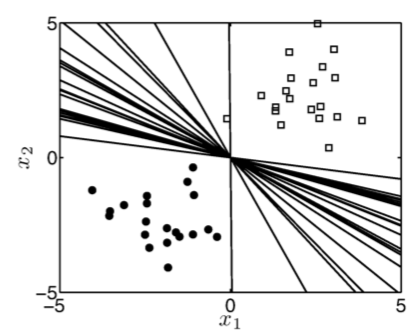
\includegraphics[width=.8\linewidth]{img/MH1}
\caption{Predictive probability contours of classifying objects as square.}
\label{MH1}
\end{subfigure}
\begin{subfigure}{.47\textwidth}
\centering
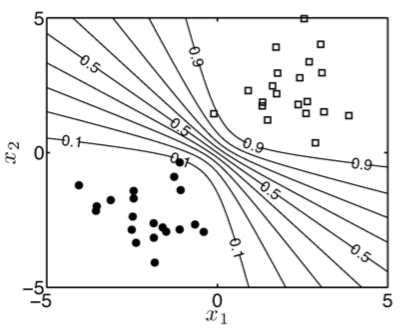
\includegraphics[width=.8\linewidth]{img/MH2}
\caption{Decision boundaries created from randomly selected MH samples.}
\label{MH2}
\end{subfigure}
\caption{Example of Metropolis-Hastings algorithm results.}
\end{figure}
\autoref{MH1} and \autoref{MH2} show an example of possible shapes of contours: it does not look too different from the Laplace ones. The only difference is that these contours are not so tight as the Laplace's ones. This suggests the probability decreases more slowly.

\paragraph{\textbf{Limitations}} The difficult mostly lies in the unknown shape of the density. When a density has two or more modes, MH moves towards the modes as these moves increase the posterior density and hence are always accepted. When close to a mode, many steps are required to move from one mode to another and this is very unlikely. We might end up exploring a mode without even knowing the other exists (see \autoref{mode1}). Another problem arises when the variables are strongly correlated (see \autoref{mode2}). Let us pick any position and propose a movement from a Gaussian with diagonal covariance (i.e., having circular contours). The shapes are very different and many samples will be rejected: the majority of moves that we sample from our proposal will involve moving steeply down the probability gradient. There are even other problems.

\begin{figure}
\begin{subfigure}{.5\textwidth}
\centering
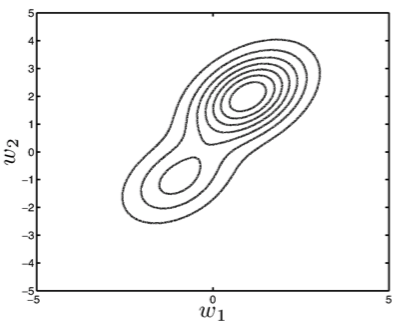
\includegraphics[width=.8\linewidth]{img/mode1}
\caption{A bi-modal density.}
\label{mode1}
\end{subfigure}
\begin{subfigure}{.5\textwidth}
\centering
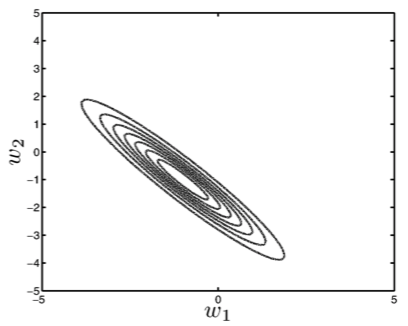
\includegraphics[width=.8\linewidth]{img/mode2}
\caption{Highly correlated parameter density.}
\label{mode2}
\end{subfigure}
\caption{Example of Metropolis-Hastings algorithm results.}
\end{figure}

\subsubsection{Usage}
LR is used as data analysis tool where the goal is to  understand the role of the input variables in explaining the outcome. Typically many models are fit in a search for a parsimonious model involving a subset of the variables, possibly with some interactions terms. 

It is widely used in biostatistical applications where binary responses (two classes) occur quite frequently. For example, patients survive or die, have heart disease or not, or a condition is present or absent.

\subsection{Regularized Logistic regression}
We can use the $L_1$ penalty for variable selection and shrinkage:

\begin{equation}
\argmax{\beta_0,\beta_1} \left\lbrace \sum_{i=1}^N y_i\left(  \beta_0 + \beta^Tx_i\right) -\log \left( 1+e^{\beta_0 + \beta^T x_i}\right) -\lambda \sum_{j=-1}^p |\beta_j|\right\rbrace
\end{equation}
This function is concave and can be solved using a nonlinear programming method.
\subsection{Logistic vs LDA}
The difference between the models relies on how the linear coefficients are estimated. The logistic regression model is more general since it makes less assumptions.

LDA is not robust to outliers since observations far from the decision boundary are used to estimate the common covariance matrix, while they are scaled down in the Logistic regression.

\subsection{Perceptron learning algorithm}
It tries to find a separate hyperplane by minimizing the distance of misclassified points to the decision boundary. If a response $y_i = 1$ is misclassified, then $x^T_i \beta + \beta_0 < 0$, and the opposite for a misclassified response with $y_i = -1$. The goal is to minimize
\begin{equation}
D(\beta, \beta_0) = - \sum_{i\in\CMcal{M}} y_i\left(x_i^T\beta + \beta_0\right)
\end{equation}
where $\CMcal{M}$ is the set of misclassified points.
The gradient is
\begin{align}
\frac{\partial D(\beta,\beta_0}{\partial \beta} = -\sum_{i\in\CMcal{M}}y_ix_i \\
\frac{\partial D(\beta,\beta_0}{\partial \beta_0} = -\sum_{i\in\CMcal{M}} y_i
\end{align}
where the algorithm uses the stochastic gradient descent where the coefficients are updated by the gradient value weighted by a step $\rho$. There are many problems though:
\begin{itemize}
\item when data are separable, there are many solutions which depend on the starting value;
\item many steps might be required;
\item when data are not separable, the algorithm will not converge;
\end{itemize}

\subsection{Optimal separating hyperplanes}
\label{OSH}
See \autoref{HardMarginSVM}.

%%%%%%%%%%%%%%%%%%%%%%%%%%%%%%%%%%%%%%%%%%%%%%%%%%%%%%%%%%
%%%%%%%%------------------------------NEW SECTION------------------------------%%%%%%%%%
%%%%%%%%%%%%%%%%%%%%%%%%%%%%%%%%%%%%%%%%%%%%%%%%%%%%%%%%%%
\newpage
\section{Basis expansion and regularization}
To extend the flexibility of linear model, a transformation of $\X$ can be performed and then use a linear model to the derived input features. Denoting the transformation $h_m(\X) : \CMcal{R}^p\rightarrow \CMcal	{R}$ for a single input $m$, we have the model:
\begin{equation}
f(\X) = \sum_{m=1}^M \beta_mh_m(\X)
\end{equation}
$h()$ are called \textbf{basis function}
Any kind of transformation can be applied: square-roots, squared (on single inputs i.e, $x_i^2$ or among different inputs $x_ix_j$), logarithmic, power functions, trigonometric, etc. 

Polynomials are more widely used but they have a limitation due to its global nature: when tweaking the  parameters to achieve a desired behaviour in a specific region, problems might arise in another region.

A solution is to consider \textbf{piecewise-polynomials} and \textbf{splines}.

\subsection{Piecewise Polynomials and splines}
For the moment $X$ is assumed one-dimensional. A piecewise polynomial function is obtained by  dividing the domain of $X$ into contiguous intervals and use a different $f$ in each interval.

Given a sequence $a=t_0<t_1<\cdots<t_{m+1}=b$, the piecewise polynomials are delimited by an adjacent pair in the sequence. So we have the following sequence of intervals:

\begin{equation}
I_\ell = \left[ t_{\ell-1}, t_\ell\right) \textit{ for } 1\le l\le m \textit{ and } \left[t_m, t_{m+1}\right]
\end{equation}
So the piecewise polynomials, having basis functions: $h_0(X) = 1, h_1(X) = X, h_2(X) = X^2$ and so on, is:

\begin{equation}
f(x) = \left\{ \begin{array}{ll} g_0(x) = \beta_{0,0} + \beta_{0,1} X + \cdots + \beta_{0,k-1} X^{k-1}\quad X \in I_1 \\ 
\vdots\\
 g_{m-1}(x) = \beta_{m-1,0} + \beta_{m-1,1} X + \cdots + \beta_{m-1,k-1} X^{k-1}\quad X \in I_{k+1} \\  \quad 
\end{array}
 \right.
\end{equation}

In this way we get discontinuities at the boundaries. Note that discontinuity means we get completely different values for almost the same input. More often we would like to have continuity at the boundaries or knots: $f(\xi^+)=f(\xi^-)$ which implies the condition:$\beta_1 +\xi\beta_2 = \beta_3 +\xi_1\beta_4$ which removes one degree of freedom.

These constrains, one for each knot, can be embedded in additional basis functions of the type $h(X) = \br{X - \xi}_+$ where $\br{\cdot}_+ = \max(\cdot, 0)$ i.e., the basis function is $0$ for $X - \xi<\xi$, $X - \xi$ otherwise
\begin{equation}
h(X) = \br{X - \xi}_+ = \max(X - \xi, 0) = \left\{ \begin{array}{ll}  0 &\quad X-\xi<0\\
X-\xi &\quad X-\xi\ge0
\end{array}
 \right.
\end{equation}

Using the previous and these basis functions we can reexpress the global function as:
\begin{equation}
\begin{aligned}
f(x) =& \beta_{0,0} + \beta_{0,1}X +\cdots+\beta_{0,k-1}  X^{k-1} + \\
&+\beta_{1,0}(X -\xi_0)_+^0     + \beta_{1,1}(X -\xi_0)_+^1       +\cdots +\beta_{1,k-1} (X -\xi_0)_+^{k-1}+  \\
&+\vdots \\ 
&+\beta_{m-1,0}(X -\xi_{m-1})_+^0 +\cdots +\beta_{m-1,k-1} (X -\xi_{m-2})_+^{k-1}
\end{aligned}
\end{equation}
\textbf{To force continuity between two regions} we set the terms $\beta_{1,0}(X -\xi_j)_+^0$ to $0$:

For example forcing continuity at the first knot:
\begin{equation}
\begin{aligned}
&\beta_{1,0}(X -\xi_0)_+^0 = \beta_{0,0} + \beta_{0,1} \xi_0\\
&\Rightarrow \beta_{1,0} = \beta_{0,0} + \beta_{0,1} \xi_0
\end{aligned}
\end{equation}

 In this way we don't have a jump at the boundaries:

\begin{equation}
\begin{aligned}
f(x) =& \beta_{0,0} + \beta_{0,1}X +\cdots+\beta_{0,k-1}  X^{k-1} + \\
&+ \beta_{1,1}(X -\xi_0)_+^1       +\cdots +\beta_{1,k-1} (X -\xi_0)_+^{k-1}+  \\
&+\vdots \\ 
&+ \beta_{m-1,1}(X -\xi_{m-1})_+^1 +\cdots +\beta_{m-1,k-1} (X -\xi_{m-1})_+^{k-1}
\end{aligned}
\end{equation}
In this way we have removed $m-1$ parameters.

There is a difference in this representation: before we have to select a polynomial function for a specific region where the fit to the global function was given by the fit of the parameters specific to that region, now we have a global function that works a little differently. In the first region, the only non-null terms are $\beta_{0,j}$ as before. When reaching the second region, the terms $\beta_{1,j}$ becomes non-null. Now the coefficients of the polynomial are the sum of the coefficients of these two region: i.e., in the second region we have:
\begin{equation}
\begin{aligned}
f(x) =& \beta_{0,0} -(\beta_{1,1}+\cdots+\beta_{1,k-1})\xi_0+ (\beta_{0,1}+\beta_{1,1})X+\\
&+\cdots+(\beta_{0,k-1}  +\beta_{1,k-1})X^{k-1}
\end{aligned}
\end{equation}

\autoref{spline_linear} shows the global function, solid line, given by the sum of basis functions, dashed lines, when traversing the graph from left to right. At each knot, a new basis function is activated and summed to the global function.

The basis functions can be seen as a correction to the global polynomial for that  specifc region and the knots are those points where the correction starts. At the knot $X=\xi_j$ so the correction starts very gently and the continuity is preserved.

\begin{figure}
\begin{subfigure}{0.49\textwidth}
\centering
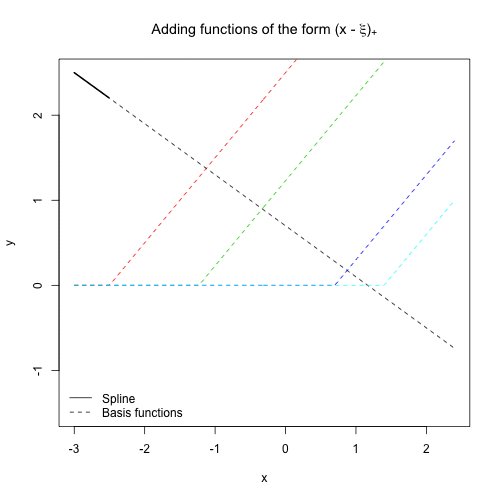
\includegraphics[width=0.9\linewidth]{img/spline_linear/10}
\caption{First region.}
\end{subfigure}
\hfill
\begin{subfigure}{0.49\textwidth}
\centering
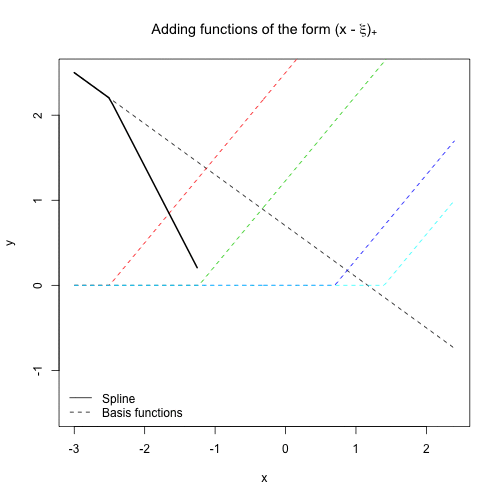
\includegraphics[width=0.9\linewidth]{img/spline_linear/33}
\caption{Second region.}
\end{subfigure}
\begin{subfigure}{0.49\textwidth}
\centering
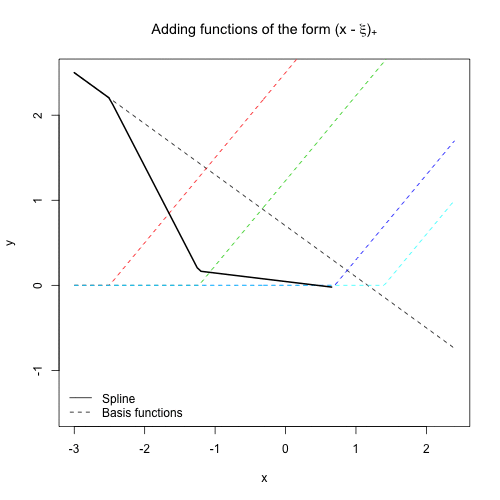
\includegraphics[width=0.9\linewidth]{img/spline_linear/68}
\caption{Third region.}
\end{subfigure}
\hfill
\begin{subfigure}{0.49\textwidth}
\centering
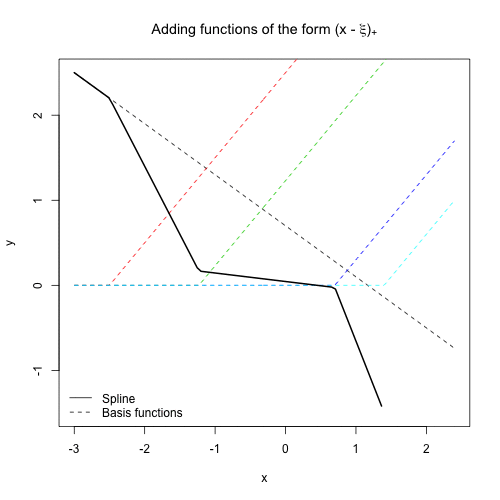
\includegraphics[width=1\linewidth]{img/spline_linear/81}
\caption{Fourth region.}
\end{subfigure}
\end{figure}
\begin{figure}\ContinuedFloat
\begin{subfigure}{0.49\textwidth}
\centering
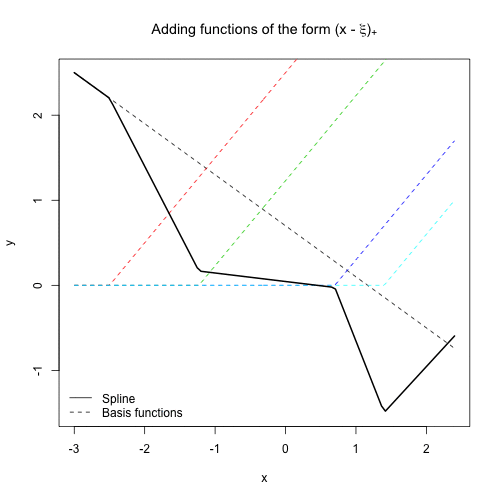
\includegraphics[width=1\linewidth]{img/spline_linear/100}
\caption{Fifth region.}
\end{subfigure}
\caption{Linear splines. The solid line is the global function while the dashed lines are the basis functions.}
\label{spline_linear}
\end{figure}

Generally, smoother functions are preferred and these are achieved by increasing the order of the local polynomials and increasing the order of continuity (continuity first derivative, second derivative). It is claimed that cubic splines are the lowest-order spline for which the discontinuity is not visible to the human eye and seldom higher degrees are needed, unless smooth derivatives are required.

The spline order, number of knots and their positions must be selected. Generally the position of the knots is chosen according the observation, while the order is chosen a-priori.

\begin{figure}
\begin{subfigure}{0.49\textwidth}
\centering
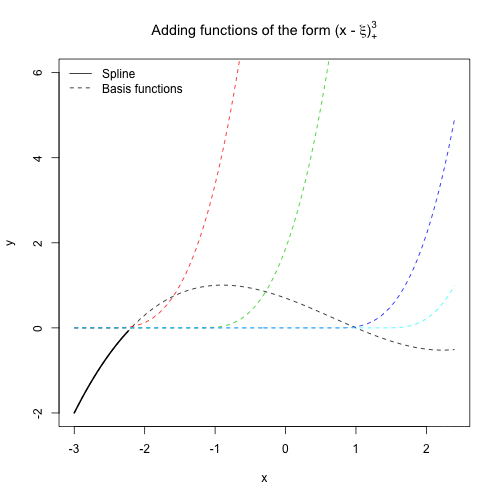
\includegraphics[width=1\linewidth]{img/spline_cubic/15}
\caption{First region.}
\end{subfigure}
\hfill
\begin{subfigure}{0.49\textwidth}
\centering
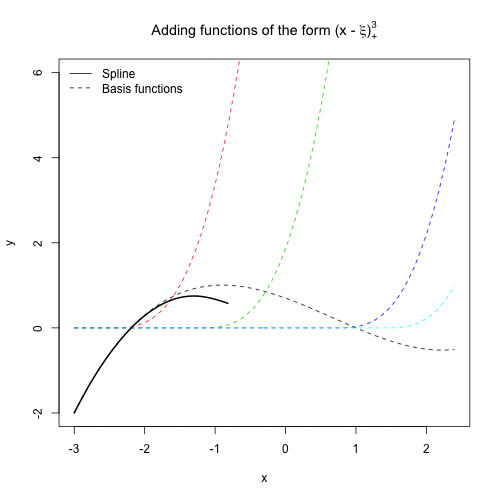
\includegraphics[width=1\linewidth]{img/spline_cubic/41}
\caption{Second region.}
\end{subfigure}
\begin{subfigure}{0.49\textwidth}
\centering
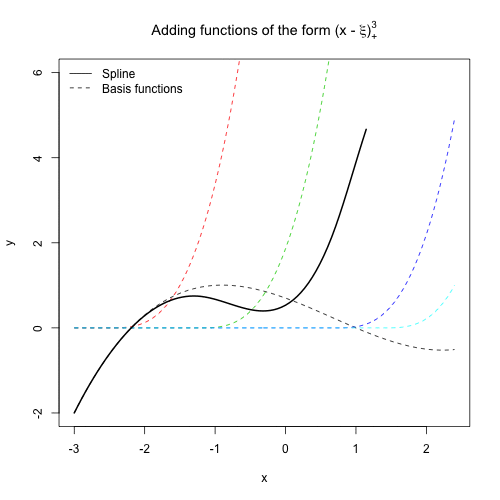
\includegraphics[width=1\linewidth]{img/spline_cubic/77}
\caption{Third region.}
\end{subfigure}
\hfill
\begin{subfigure}{0.49\textwidth}
\centering
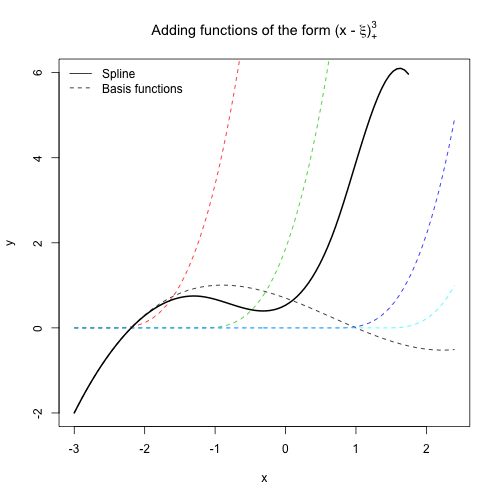
\includegraphics[width=1\linewidth]{img/spline_cubic/88}
\caption{Fourth region.}
\end{subfigure}
\end{figure}
\begin{figure}\ContinuedFloat
\begin{subfigure}{0.49\textwidth}
\centering
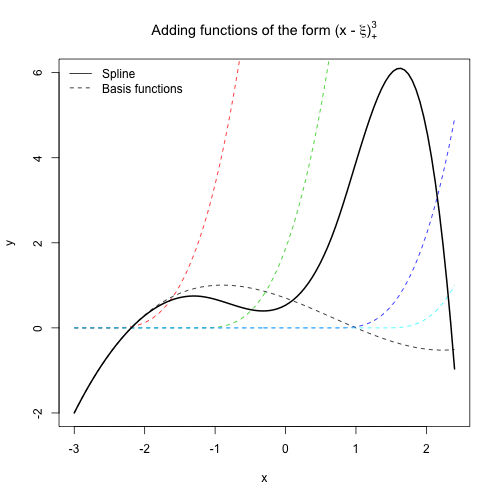
\includegraphics[width=1\linewidth]{img/spline_cubic/100}
\caption{Fifth region.}
\end{subfigure}
\label{spline_cubic}
\caption{Cubic splines. The solid line is the global function while the dashed lines are the basis functions.}
\end{figure}

\subsection{Natural cubic splines}
Polynomial fits to data tends to be erratic at the boundaries and additionally splines behave even more widely than the global polynomial beyond the boundaries. This is shown by the point-wise variance (the variance of the estimator at one point: $\Var[\hat{f}(x_0)]$ in \autoref{pointwise_var}. Note the variance explosion close to the boundaries, especially for cubic splines.

\begin{figure}
\centering
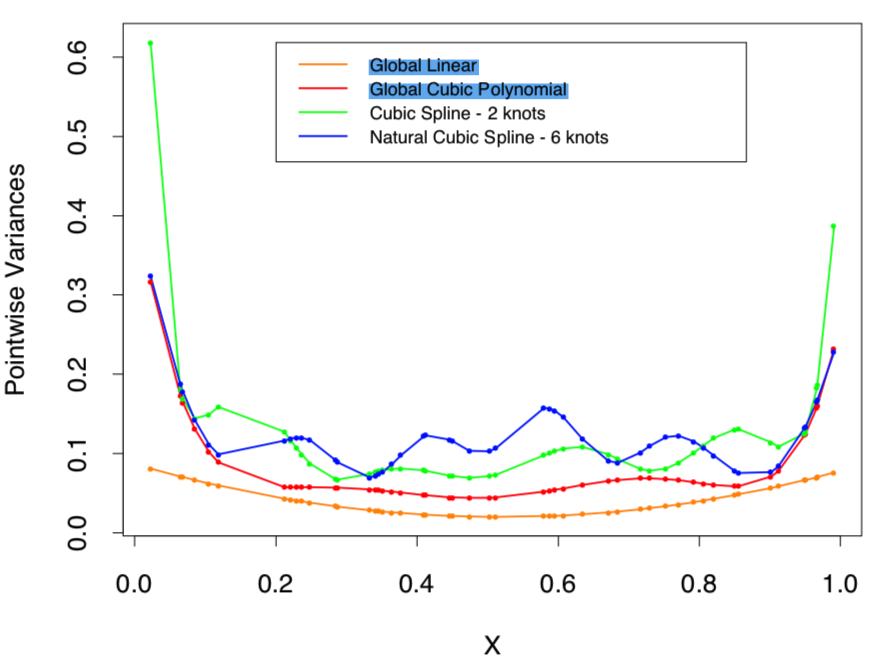
\includegraphics[scale=0.4]{img/pointwise_var}
\caption{$X$ consists of 50 points drawn randomly from $U[0,1]$ and an assumed error model of with constant variance. Both cubic splines have 6 degrees of freedom. The cubic spline has two knots at $0.33$ and at $0.66$ while the natural cubic spline has boundary knots at $0.1$ and $0.9$, and four interior knots uniformly spaced between them.}
\label{pointwise_var}
\end{figure}

A  \textbf{natural cubic spline} adds additional constraints by forcing linearity beyond the boundary knots. These frees up four degrees of freedom (2 in both boundary regions), that can be used more profitably by sprinkling more knots in the interior region. There will be a price to pay in terms of bias near the boundaries, but in these regions we have less information anyway so assuming the function is linear here is reasonable.

A natural cubic spline with $K$ knots is represented by $K$ basis functions. One can start from the basis of a cubic spline and then derive the reduce basis by imposing the boundary constraints.

Starting from the general continuous basis for four regions (four knots):
\begin{equation}
\begin{aligned}
&h_1(X) =1, \quad\quad\quad h_2(X) =X,\quad h_3(X) =X^2,\quad  h_4(X) = X^3,\\
&h_5(X) = X-\xi_0,\quad h_6(X) = (X-\xi_0)^2,\quad, h_7(X) = (X-\xi_0)^3\\
&h_8(X) = X-\xi_1,\quad h_9(X) = (X-\xi_1)^2,\quad h_{10}(X) = (X-\xi_1)^3\\
&h_9(X) = X-\xi_2,\quad h_10(X) = (X-\xi_1)^2,\quad h_{11}(X) = (X-\xi_2)^3
\end{aligned}
\end{equation}
Enforcing also continuity of the first and second derivatives at the knots we reduce the basis to:
\begin{equation}
\begin{aligned}
&h_1(X) = 1, \quad h_2(X) =X,\quad h_3(X) =X^2,\quad  h_4(X) = X^3,\\
&h_5(X) = (X-\xi_0)^3, \quad h_6(X) = (X-\xi_1)^3, \quad h_7(X) = (X-\xi_2)^3.
\end{aligned}
\end{equation}

Enforcing linearity beyond the boundaries, we eliminate $ h_3(X)$ and $ h_4(X)$. We must also keep the cubic expression in the intermediate regions but somehow make the cubic part cancel out when reaching the fifth region since here it must be linear. We can add for each region in the interval $[1, K-2]$ the following basis function:
\begin{equation}
\begin{aligned}
&h_k(X) = d_k(X) - d_{K-1}(X)\\
\textit{where} \quad &d_k(X) = \frac{\br{X-\xi_k}_+^3 - \br{X-\xi_K}_+^3 }{\xi_K - \xi_k}
\end{aligned}
\end{equation}

In the first region we have:
\begin{equation}
\hat{f}_1(X) = \beta_0 + \beta_1 X
\end{equation}
In the second region we have:
\begin{equation}
\begin{aligned}
&\hat{f}_2(X) = \beta_0 + \beta_1 X +\beta_2 \frac{(X-\xi_0)^3}{\xi_2 - \xi_0} =\\
&= \beta_0 + \beta_1 X +\beta_2 \frac{X^3 -3 \xi_0 X^2 + 3\xi_0^2 X-\xi_0^3}{\xi_2 - \xi_0} =\\
&= \frac{\beta_2}{\xi_2 - \xi_0} X^3 -3 \beta_2\frac{\xi_0}{\xi_2 - \xi_0} X^2 + (\beta_1+3\beta_2\frac{\xi_0^2}{\xi_2 - \xi_0})X + \beta_0 - \beta_2\frac{\xi_0^3}{\xi_2 - \xi_0}
\end{aligned}
\end{equation}
In the third region we have:
\begin{equation}
\begin{aligned}
&\hat{f}_3(X) = \beta_0 + \beta_1 X  +\beta_2 h_2(X) = \beta_0 + \beta_1 X  +\beta_2\left[ \frac{(X-\xi_0)^3}{\xi_2 - \xi_0} - \frac{(X-\xi_1)^3}{\xi_2 - \xi_1}\right]  \\
&= \beta_0 + \beta_1 X +\beta_2 \left[ \frac{X^3 -3 \xi_0 X^2 + 3\xi_0^2 X-\xi_0^3}{\xi_2 - \xi_0} -  \frac{X^3 -3 \xi_1 X^2 + 3\xi_1^2 X-\xi_1^3}{\xi_2 - \xi_1}\right] =\\
&= \beta_0 + \beta_1 X +\beta_2 \frac{(\xi_2-\xi_1-\xi_2+\xi_0)X^3-3\left[ \xi_0(\xi_2-\xi_1) - \xi_1(\xi_2-\xi_0)\right]X^2}{(\xi_2 - \xi_0)(\xi_2 - \xi_1)}+\\
&\quad +  \frac{3\left[\xi_0^2(\xi_2-\xi_1) - \xi_1^2(\xi_2-\xi_0) \right]X-\left[(\xi_0^3(\xi_2-\xi_1) -\xi_1^3(\xi_2-\xi_0)\right]}{(\xi_2 - \xi_0)(\xi_2 - \xi_1)}=\\
&=  \beta_0 + \beta_1 X +\beta_2 \frac{(-\xi_1+\xi_0)X^3-3\xi_2(\xi_0-\xi_1)X^2}{(\xi_2 - \xi_0)(\xi_2 - \xi_1)}+\\
&\quad +  \frac{3\left[\xi_2(\xi_0-\xi_1)(\xi_0+\xi_1)-\xi_0\xi_1(\xi_0-\xi1)\right]X}{(\xi_2 - \xi_0)(\xi_2 - \xi_1)}+\\
&\quad\quad-\frac{\left[\xi_2(\xi_0-\xi_1)(\xi_0^2-\xi_0\xi_1+\xi_1^2)-\xi_0\xi_1(\xi_0-\xi1)(\xi_0+\xi_1)\right]}{(\xi_2 - \xi_0)(\xi_2 - \xi_1)} = \\
&=\beta_0 + \beta_1 X -\beta_2 (\xi_1-\xi_0)\frac{X^3-3\xi_2X^2}{(\xi_2 - \xi_0)(\xi_2 - \xi_1)}+\\
&\quad\quad +  \frac{3\left[\xi_2(\xi_0+\xi_1)-\xi_0\xi_1\right]X-\left[\xi_2(\xi_0^2-\xi_0\xi_1+\xi_1^2)-\xi_0\xi_1(\xi_0+\xi_1)\right]}{(\xi_2 - \xi_0)(\xi_2 - \xi_1)}=\\
&= -\beta_2\frac{(\xi_1-\xi_0)}{(\xi_2 - \xi_0)(\xi_2 - \xi_1)} X^3 +3 \beta_2\frac{\xi_2(\xi_1-\xi_0)}{(\xi_2 - \xi_0)(\xi_2 - \xi_1)} X^2 + \\
&\quad\quad +(\beta_1-3\beta_2(\xi_1-\xi_0)\frac{\xi_2(\xi_0+\xi_1)-\xi_0\xi_1}{(\xi_2 - \xi_0)(\xi_2 - \xi_1)})X +\\
&\quad\quad+ \beta_0 + \beta_2(\xi_1-\xi_0)\frac{\xi_2(\xi_0^2-\xi_0\xi_1+\xi_1^2)-\xi_0\xi_1(\xi_0+\xi_1)}{(\xi_2 - \xi_0)(\xi_2 - \xi_1)}
\end{aligned}
\end{equation}
In the fourth region:
\begin{equation}
\begin{aligned}
&\hat{f}_3(X) = \beta_0 + \beta_1 X  +\beta_2 h_2(X) =\\
&= \beta_0 + \beta_1 X  +\beta_2\left[ \frac{(X-\xi_0)^3-(X-\xi_2)^3}{\xi_2 - \xi_0} - \frac{(X-\xi_1)^3-(X-\xi_2)^3}{\xi_2 - \xi_1}\right]  \\
&= \beta_0 + \beta_1 X +\beta_2 \frac{X^3 -3 \xi_0 X^2 + 3\xi_0^2 X-\xi_0^3-X^3 +3 \xi_2 X^2 - 3\xi_2^2 X+\xi_2^3}{\xi_2 - \xi_0} +\\
&\quad\quad\quad -\beta_2  \frac{X^3 -3 \xi_1 X^2 + 3\xi_1^2 X-\xi_1^3-X^3 +3 \xi_2 X^2 - 3\xi_2^2 X+\xi_2^3}{\xi_2 - \xi_1} =\\
&= \beta_0 + \beta_1 X +\beta_2 \frac{ 3 (\xi_2-\xi_0) X^2 - 3(\xi_2^2- \xi_0^2) X+\xi_2^3-\xi_0^3}{\xi_2 - \xi_0} +\\
&\quad\quad\quad -\beta_2         \frac{3 (\xi_2-\xi_1 ) X^2 - 3(\xi_2^2 - \xi_1^2) X+\xi_2^3-\xi_1^3  }{\xi_2 - \xi_1} =\\
&= \beta_0 + \beta_1 X +\beta_2 \frac{ \cancel{3(\xi_2 - \xi_1) (\xi_2-\xi_0) X^2} - 3(\xi_2 - \xi_1)(\xi_2^2- \xi_0^2) X+(\xi_2 - \xi_1)(\xi_2^3-\xi_0^3)}{(\xi_2 - \xi_0)(\xi_2 - \xi_1)} +\\
&\quad\quad\quad -\beta_2         \frac{\cancel{3 (\xi_2 - \xi_0)(\xi_2-\xi_1 ) X^2} - 3(\xi_2 - \xi_0)(\xi_2^2 - \xi_1^2) X+(\xi_2 - \xi_0)(\xi_2^3-\xi_1^3  )}{(\xi_2 - \xi_0)(\xi_2 - \xi_1)} =\\
&= \beta_0 + \beta_1 X +\beta_2 \frac{- 3(\xi_2 - \xi_1)(\xi_2^2- \xi_0^2) X+(\xi_2 - \xi_1)(\xi_2^3-\xi_0^3)}{(\xi_2 - \xi_0)(\xi_2 - \xi_1)} +\\
&\quad\quad\quad -\beta_2         \frac{- 3(\xi_2 - \xi_0)(\xi_2^2 - \xi_1^2) X+(\xi_2 - \xi_0)(\xi_2^3-\xi_1^3  )}{(\xi_2 - \xi_0)(\xi_2 - \xi_1)} =\\
&= \beta_0 + \beta_1 X +\beta_2 \frac{3\left[-\xi_2(\xi_1^2-\xi_0^2)+\xi_2^2(\xi_1-\xi_0)+\xi_0\xi_1(\xi_1-\xi_0)\right]X+}{(\xi_2 - \xi_0)(\xi_2 - \xi_1)}\\
&\quad\quad \frac{-\xi_2(\xi_1^3-\xi_0^3)-\xi_2^3(\xi_1-\xi_0)-\xi_0\xi_1(\xi_1-\xi_0)}{(\xi_2 - \xi_0)(\xi_2 - \xi_1)}
\end{aligned}
\end{equation}
Note that the fourth region is linear.
\subsection{Smoothing splines}
We can avoid knot selection by using a maximal set of knots, controlled by a regularization process. The problem is: \textit{Among all functions $f(x)$ with two continuous derivatives, find the one that minimizes the penalized residual sum of squares}:
\begin{equation}
RSS(f,\lambda) = \sum_{i=1}^N \left[y_i - f(x_i)\right]^2 + \lambda \int f''(t) dt
\label{RSSspl}
\end{equation}
The first term measures closeness to the data, while the second term penalizes curvature in the function. If $\lambda=0$ $f$ can be any function that interpolates the data so we can achieve smoothness. If $\lambda=\infty$ simple least squares line fit, since no second derivative can be tolerated and we get a "rough" function.
\autoref{RSSspl} has an explicit finite-dimensional unique minimizer which is a natural cubic spline with knots at the unique values of the $x_i$, $i = 1,...,N$, so there are as many as $N$ knots, hence $N$ degrees of freedom. The penalty translates to a penalty on the spline coefficients, which are shrunk to the linear fit.

Being the solution a natural spline, we can write it as:
\begin{equation}
f(x) = \sum_{j=1}^N N_j(x)\theta_j
\end{equation}
where $N_j(x)$ are the N-dimensional set of basis functions for representing this family of natural splines:
\begin{equation}
RSS(\theta, \lambda) = \br{\y - \mathbf{N}\theta}^T\br{\y - \mathbf{N}\theta}+\lambda \theta^T\mathbf{\Sigma_N}\theta
\end{equation}
where ${N}_{i,j} = N_j(x_i)$ and $${\mathbf{\Sigma_N}}_{j,k} = \int N_j''(t)N_k''(t)dt$$. The solution is :
\begin{equation}
\hat{\theta} = \br{\mathbf{N}^T\mathbf{N}+\lambda\mathbf{\Sigma}_N}^{-1}\mathbf{N}^T\y = \mathbf{S_\lambda} \y
\end{equation}
which is a generalized ridge regression. $\mathbf{S_\lambda}$ is positive-definite, symmetric and $\mathbf{S_\lambda}\mathbf{S_\lambda} \le \mathbf{S_\lambda}$. Since it is symmetric and positive-definite it has a real eigenvalue decomposition. Let us re-write $\mathbf{S_\lambda} = \br{\I-\lambda \mathbf{K}}^{-1}$.
The eigenvalue decomposition of $\mathbf{S_\lambda}$ is:
\begin{equation}
\begin{aligned}
\mathbf{S_\lambda} = \sum_{k=1}^N \rho_k(\lambda)\mathbf{u}_k\mathbf{u}_k^T\\
\rho_k(\lambda) = \frac{1}{1+\lambda d_k}
\end{aligned}
\end{equation}
The degrees of freedom are $df_\lambda = Tr(\mathbf{S_\lambda})$.

The eigenvectors are not affected by changes in $\lambda$, and hence the whole family of smoothing splines for a particular sequence of $x$, indexed by $\lambda$ have the same eigenvectors.
$\mathbf{S_\lambda} \y= \sum_{k=1}^N \mathbf{u}_k\rho_k(\lambda)\langle\mathbf{u}_k,\y\rangle$: the smoothing spline decomposes $\y$ w.r.t. the complete basis $\mathbf{u}_k$ and differently shrinking the contributions using $\rho_k(\lambda)$. 
So for example suppose $\mathbf{B}_xi$ is a matrix of cubic-splines basis functions. Then the vector of fitted spline values is given by $\hat{f} = \mathbf{B}_\xi (\mathbf{B}_\xi^T\mathbf{B}_\xi)^{-1} \mathbf{B}_\xi^T\y = \mathbf{H}_\xi \y$.In such a basis regression method the contributions are either left alone or shrunk to $0$. The first two eigenvalues are always $1$ and they correspond to the two-dimensional eigenspace of functions linear in $x$ which are never shrunk. The eigenvalues $\rho_k(\lambda) = 1/(1 + \lambda dk)$ are an inverse function of the eigenvalues $d_k$ of the penalty matrix $\mathbf{K}$, moderated by $\lambda$; $\lambda$ controls the rate at which the $\rho_k(\lambda)$ decrease to zero. $d1 = d2 = 0$ and again linear functions are not penalized.

\subsection{Multidimensional splines}
Suppose $X \in \CMcal{R}^2$ and suppose we have two sets: $h_{1,k}(X_1), k=1,\cdots, M_1$ for representing functions of coordinate $X_1$, and a set of $M_2$ functions $h_{2,k}(X_2)$ for coordinate $X_2$. Then the$M_1\times M_2$ dimensional tensor product basis defined by:
\begin{equation}
g_{j,k} = h_{1,j}(X_1)h_{2,k}(X_2), \quad j=1,\cdots, M_1, \quad k=1,\cdots, M_2 
\end{equation}
can be used for representing a two-dimensional function:
\begin{equation}
g(X) = \sum_{j=1}^{M_1}\sum_{k=1}^{M_2} \theta_{jk}g_{jk}(X)
\end{equation}

The coefficients can be fit with least squares. This can be generalized to d dimensions, but note that the dimension of the basis grows exponentially fast.

One-dimensional smoothing splines (via regularization) generalize to high- er dimensions as well. Suppose we have pairs $y_i,x_i$ with $x_i \in \CMcal{R}^d$, and we seek a d-dimensional regression function $f(x)$. The idea is to set up the problem:
\begin{equation}
min_f \sum_{i=1}^N \left[y_i - f(x_i)\right]^2 +\lambda J\left[f\right]
\end{equation}
where $J$ is an appropriate penalty functional for stabilizing a function f in $\CMcal{R}^d$. For example:
\begin{equation}
 J\left[f\right] = \int \int_{\CMcal{R}^2} \left[ \left( \frac{\partial^2 f(x)}{\partial x_1^2} \right)^2+2\left(\frac{\partial^2 f(x)}{\partial x_1 \partial x_2} \right)^2+\left(\frac{\partial^2 f(x)}{\partial x_2^2} \right)^2\right]dx_1dx_2
\end{equation}
If $\lambda\rightarrow 0$ the solution approaches an interpolating function, as $\lambda$ the solution approaches the least squares plane.
The solution has the form:
\begin{equation}
f(x) = \beta_0 + \beta^T x + \sum^N_{j=1} \alpha_j h_j(x)
\end{equation}

Additive spline model can be represented in this formulation too: there exists a penalty $J[f]$ that guarantees that the solution has the from $f(X) = \alpha + f_1(X_1) +\cdots + f_d(X_d)$ and that each of the functions $f_j$ are univariate splines. In this case it is better to assume $f$ is additive and impose an additional penalty and impose an additional penalty on each of the component functions:
\begin{equation}
\begin{aligned}
J[f] = J[f_1+f_2+\cdots+f_d) =\sum_{j=1}^d \int f_j''(t_j)dt_j
\end{aligned}
\end{equation}
These are naturally extended to ANOVA spline decomposition:
\begin{equation}
f(X) = \alpha + \sum_j f_j(X_j) + \sum_{j<k} f_{jk(X_j, X_k}+ \cdots
\end{equation}
where each of the components are splines of the required dimension. There are many choices to be made:
\begin{itemize}
\item maximum order of interaction (the one above is up to order 2);
\item which term to include
\item the representation to use (regression splines with a small number of basis functions and their tensor product for interaction or a complete basis as in smoothing splines and include appropriate regularizers for each term in the expansion.
\end{itemize}

When the number of potential dimensions is large automatic methods are desirable (for example MARS and MART procedures).
\subsection{Wavelet smoothing}
$\cdots$

%%%%%%%%%%%%%%%%%%%%%%%%%%%%%%%%%%%%%%%%%%%%%%%%%%%%%%%%%%
%%%%%%%%------------------------------NEW SECTION------------------------------%%%%%%%%%
%%%%%%%%%%%%%%%%%%%%%%%%%%%%%%%%%%%%%%%%%%%%%%%%%%%%%%%%%%
\newpage
\section{Kernel smoothing methods}
\subsection{One-dimensional kernel smoothers}
We have seen the \textit{k-nearest neighbourhood} average as an estimate of the regression function $\E(Y|X=x)$:
\begin{equation}
\hat{f} = Ave(y_i|x_i\in N_k(x))
\end{equation}
where $N_k(x)$ is the set of $k-points$ nearest to $x$ in squared distance. An example of the resulting fitting curve is shown in green on the left of \autoref{nearest}. The green curve is bumpy, since $\hat{f}(x)$ is discontinuous in $x$. As we move $x_0$ from left to right, the k-nearest neighborhood remains constant, until a point $x_i$ to the right of $x_0$ becomes closer than the furthest point $x_{i'}$ in the neighbourhood to the left of $x_0$, at which time $x_i$ replaces $x_{i'}$. 
\begin{figure}
\centering
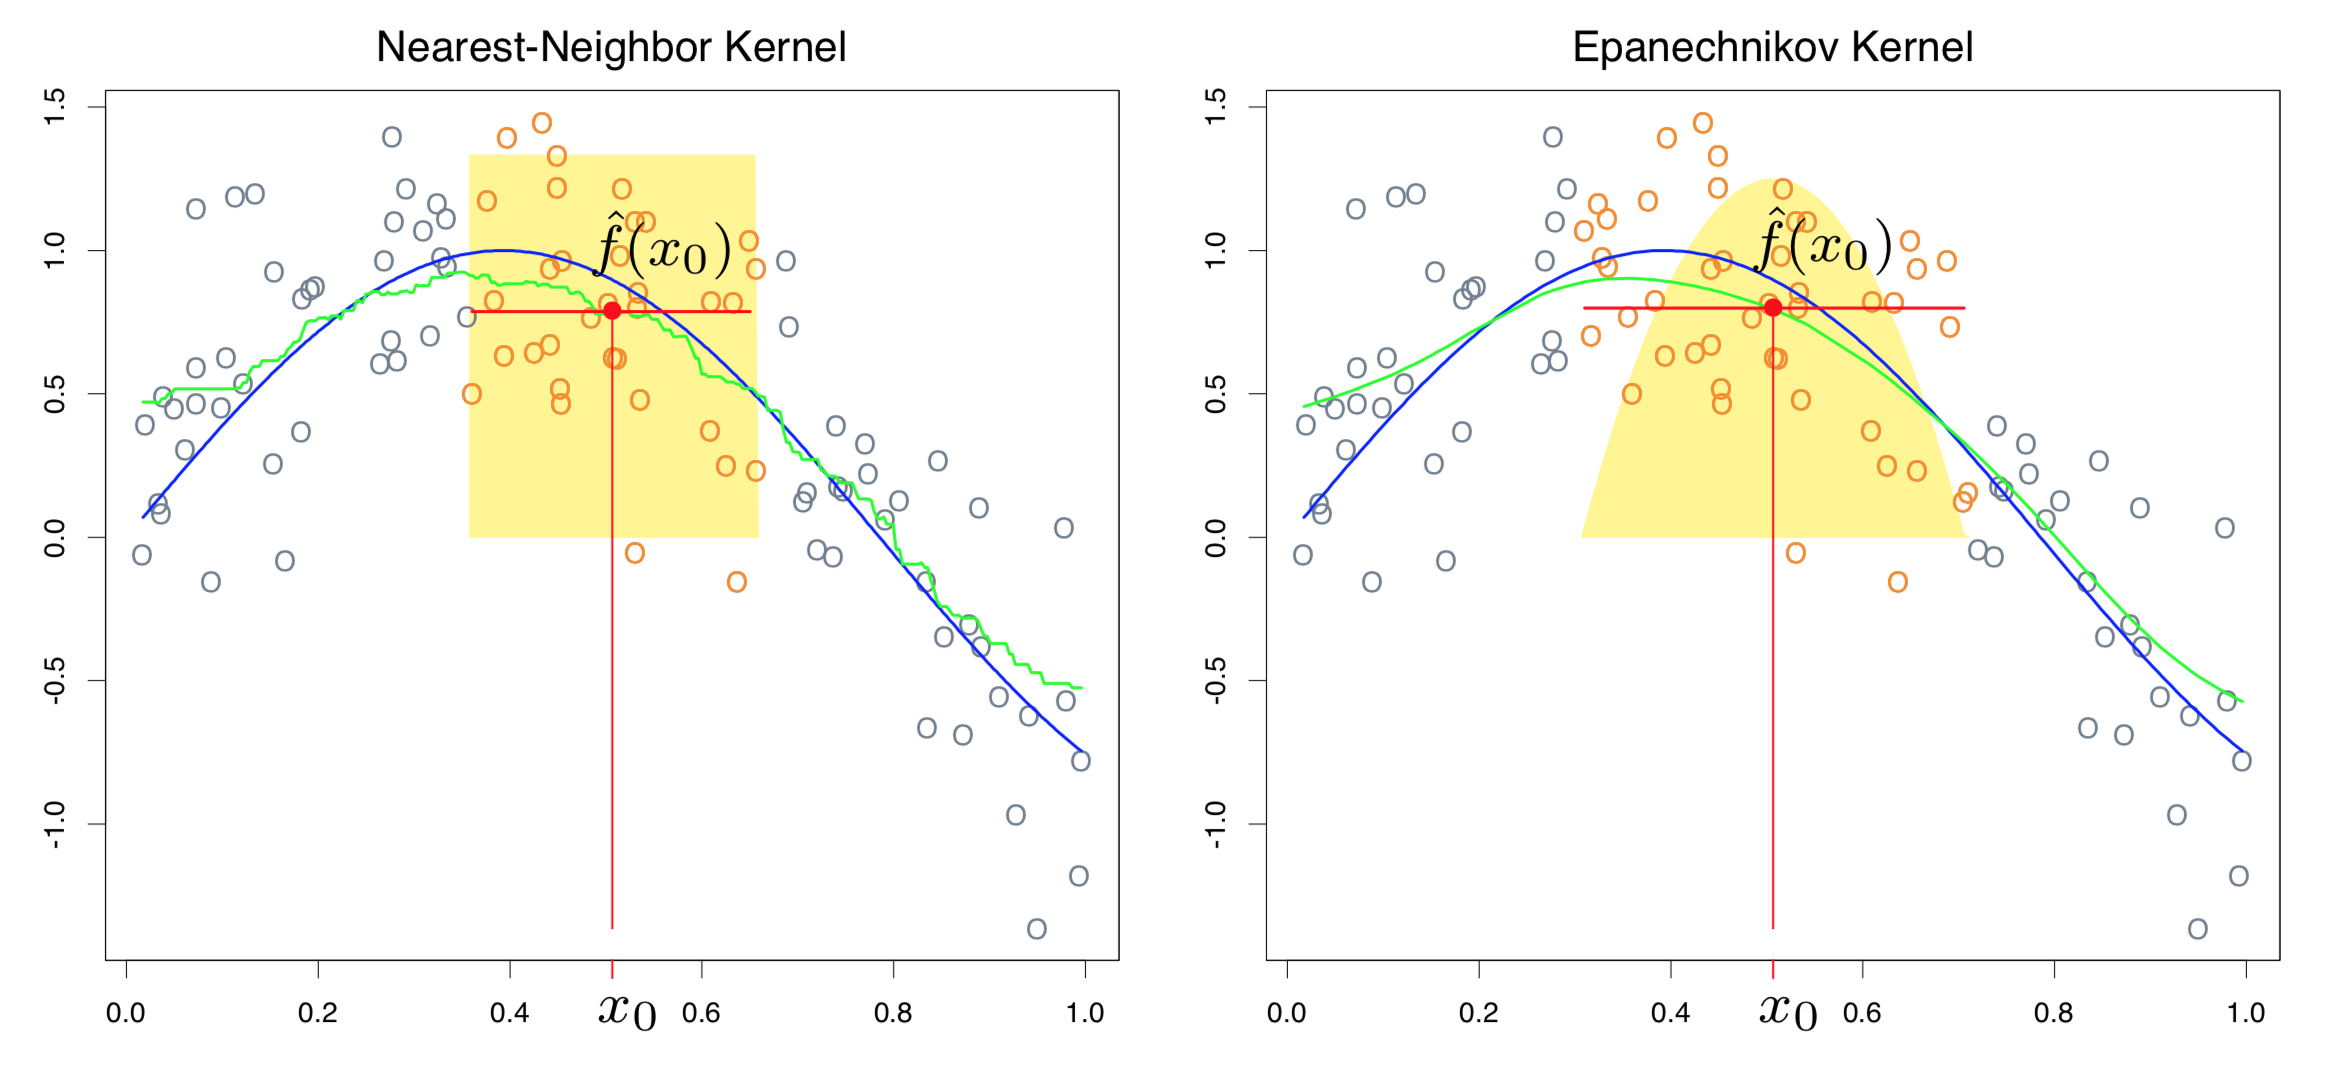
\includegraphics[scale=0.38]{img/nearest}
\caption{In green the fitting curves. On the left the one resulting from \textit{k-nearest neighbourhood}, on the right the metric neighbourhood.}
\label{nearest}
\end{figure}

Rather than give all the points in the neighbourhood equal weights, we can assign weights that die off smoothly with distance from the target point. The right panel in \autoref{nearest} shows an example of this, using the so-called Nadaraya–Watson kernel-weighted average:
\begin{equation}
\hat{f}(x) = \frac{K_\lambda(x_0, x_i)y_i}{\sum_{i=1}^N K_\lambda(x_0, x_i)}
\end{equation}
with the Epanechnikov quadratic kernel:
\begin{equation}
K_\lambda(x_0, x_i)= D\br{\frac{|x-x_0|}{\lambda}} = \left\{ \begin{array}{ll}  \frac{3}{4}\left[1-\left(\frac{|x-x_0|}{\lambda} \right)^2 \right]&\quad if \frac{|x-x_0|}{\lambda}\le 1\\
0 &\quad otherwise
\end{array}
 \right.
\end{equation}
Now the function is continuous. As we move the target from left to right, points enter the neighborhood initially with weight zero, and then their contribution slowly increases. Note that $\lambda$ dictates the width of the window which is fixed. On the contrary, for the \textit{k-nearest neighbourhood} the window size depends on the density since anyway $k$ points must be considered. \autoref{kernels} shows other kernels. Another popular one is the tri-cube function:

\begin{equation}
 D\br{\frac{|x-x_0|}{\lambda}} = \left\{ \begin{array}{ll}  \left[1-\left(\frac{|x-x_0|}{\lambda} \right)^3 \right]^3&\quad if \frac{|x-x_0|}{\lambda}\le 1\\
0 &\quad otherwise
\end{array}
 \right.
\end{equation}

Both are compact functions. A common non-compact function is the Gaussian function.

Generalizing we can use a width function $h_\lambda(x_0)$ that determines the width of the neighbourhood at $x_0$ (previously we have used $h_\lambda(x_0) = \lambda$.

\begin{figure}
\centering
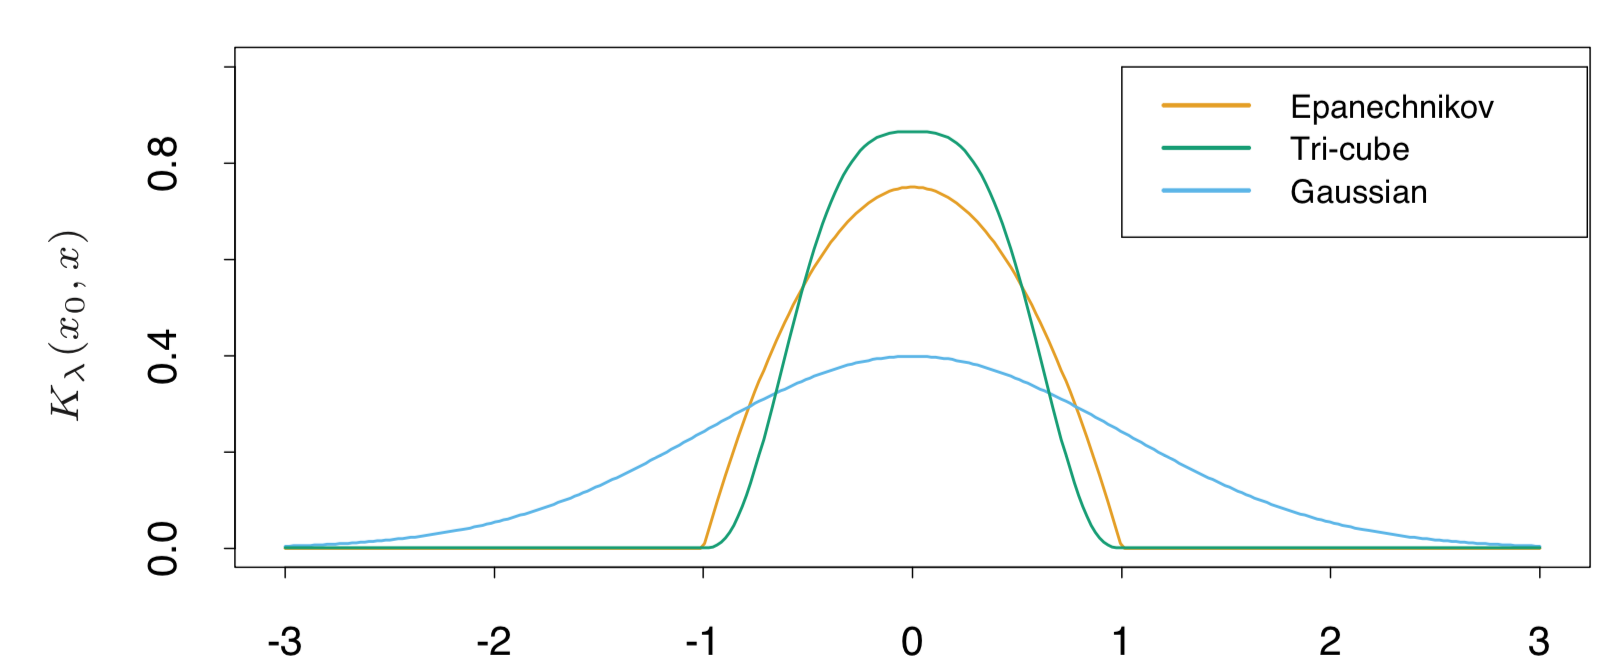
\includegraphics[scale=0.4]{img/kernels}
\caption{A comparison of three popular kernels for local smoothing. Each has been calibrated to integrate to 1. The tri-cube kernel is compact and has two continuous derivatives at the boundary of its support, while the Epanechnikov ker- nel has none. The Gaussian kernel is continuously differentiable, but has infinite support.}
\label{kernels}
\end{figure}

There are a number of details to be clarified:
\begin{itemize}
\item the value of $\lambda$ which selects the window size. Large values imply lower variance but higher bias;
\item $h_\lambda(x_0)$ can be constant (i.e., $h_\lambda(x_0)=\lambda$) or variable. Constant values (\textbf{metric window widths} keep the bias constant but the variance is inversely proportional to the local density. Nearest neighbourhood has opposite behaviour: the variance stays constant and the absolute bias varies inversely with local density.
\item boundary issues: the metric neighbourhood tend to contain less points on the boundaries while the nearest-neighbourhood get wider.
\end{itemize}

\subsubsection{Local linear regression}
Smooth kernel fit still has a problem close to the boundaries: because of the asymmetry in this region weighted averages can be badly biased (left in \autoref{biasedKernel}). By fitting straight lines rather than constants locally, we can remove this bias effect. Actually, this bias can be present in the interior of the domain as well, if the $X$ values are not equally spaced.
\begin{figure}
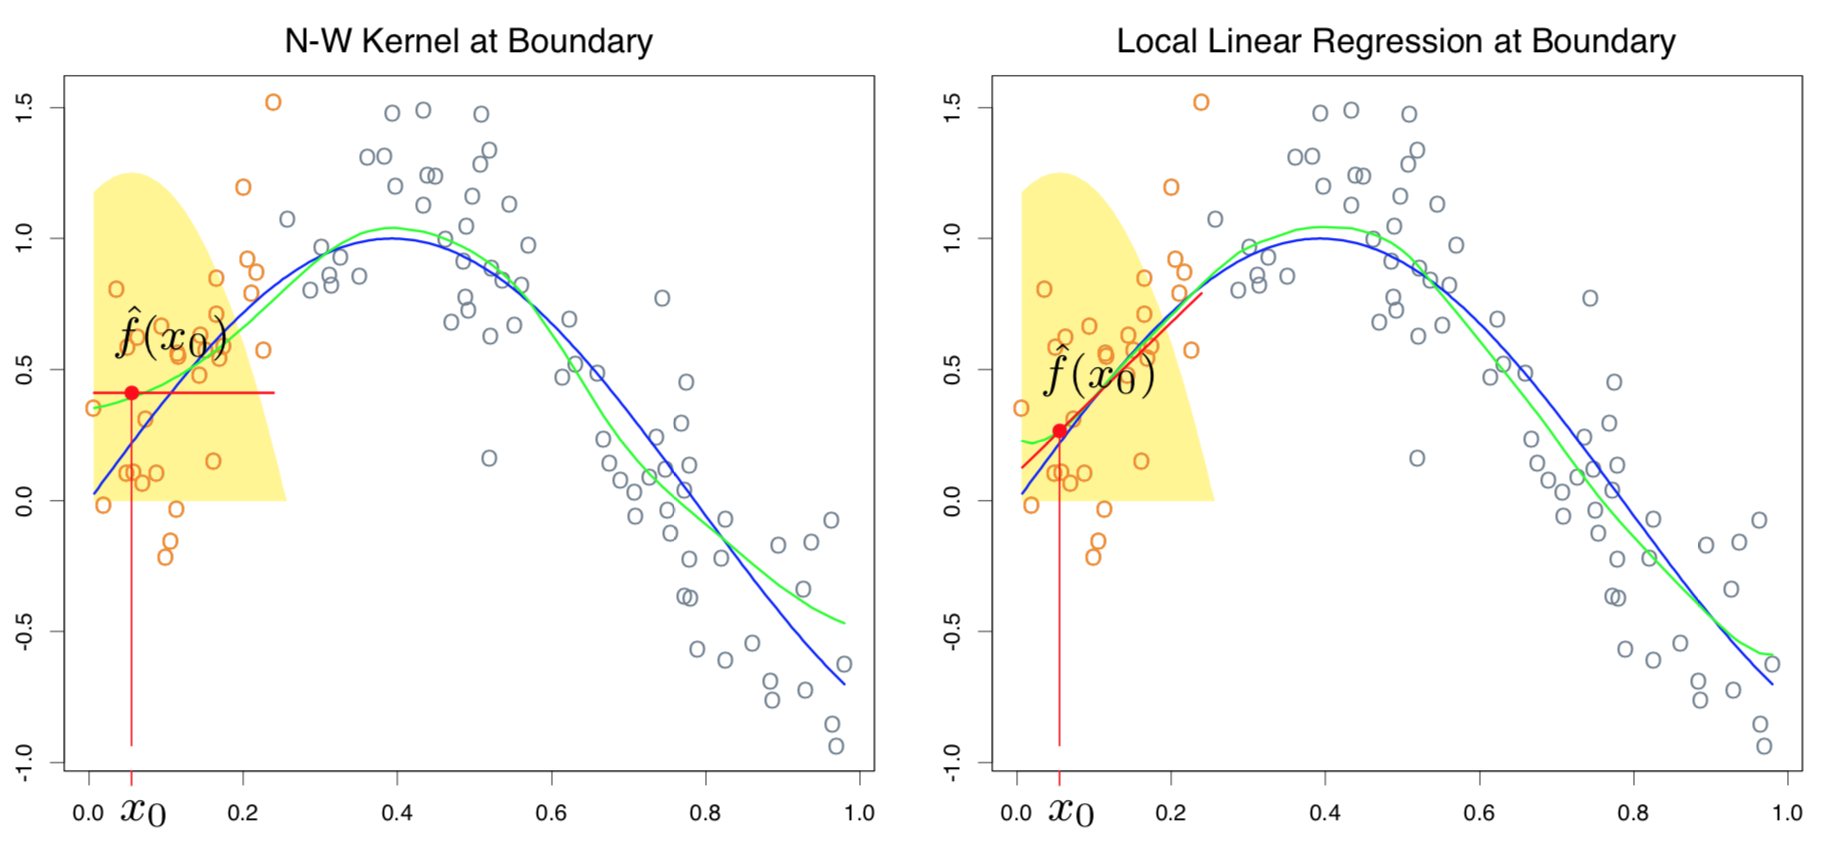
\includegraphics[scale=0.4]{img/biasedKernel}
\caption{On the left it can be noticed the bias effect at the boundaries.}
\label{biasedKernel}
\end{figure}
Locally weighted regression solves a separate weighted least squares problem at each target point $x_0$:
\begin{equation}
min_{\alpha(x_0), \beta(x_0)} \sum_{i=1}^N K_\lambda(x_0,x_1)\left[ y_i - \alpha(x_0) -\beta(x_0)x_i\right]^2
\end{equation}
and the estimate becomes:
\begin{equation}
\hat{f}(x_0) = \hat{\alpha}(x_0) + \hat{\beta}(x_0) x_0
\end{equation}
Notice that although we fit an entire linear model to the data in the region, we only use it to evaluate the fit at the single point $x_0$.

Define the vector-valued function $b(x)^T = (1, x)$. Let $B$ be the $N \times 2$ regression matrix with i-th row $b(x_i)^T$ , and $W(x_0)$ the $N \times N$ diagonal matrix with $i-th$ diagonal element $K_\lambda(x_0,x_i)$. Then
\begin{equation}
\hat{f}(x_0)= b(x_0)^T(\mathbf{B}^T\mathbf{W}(x_0)\mathbf{B})^{-1} \mathbf{B}^T\mathbf{W}(x_0)\y= \sum_{i=1}^N l_i(x_0)y_i
\end{equation}
The weights $l_i(x_0)$ combine the weighting kernel $K_\lambda(x_0, \cdot)$ and the least squares operations and are referred to as the equivalent kernel.Local linear regression automatically modifies the kernel to correct the bias exactly to
first order, a phenomenon dubbed as \textbf{automatic kernel carpentry}.

\subsubsection{Local polynomial regression}
We can fit local polynomial fits of any degree $d$:
\begin{equation}
\begin{aligned}
&min_{\alpha(x_0),\beta_j(x_0),j=1,\cdots,d} \sum_{i=1}^N K_\lambda(x_0,x_i)\left[ y_i - \alpha_0 -\sum_{j=1}^d\beta_j(x_0)x_i^j\right]^2\\
&\hat{f} = \hat{\alpha}(x_0) + \sum_{j=1}^d \hat{\beta}_j(x_0)x_0^j
\end{aligned}
\end{equation}
Local linear fits tend to be biased in regions of curvature of the true function, a phenomenon referred to as \textbf{trimming the hills} and \textbf{filling the valleys}. Local quadratic regression is generally able to correct this bias. There is of course a price to be paid for this bias reduction, and that is increased variance. The fit in the right panel of \autoref{localLinQuad} is slightly more
wiggly, especially in the tails.
\begin{figure}
\centering
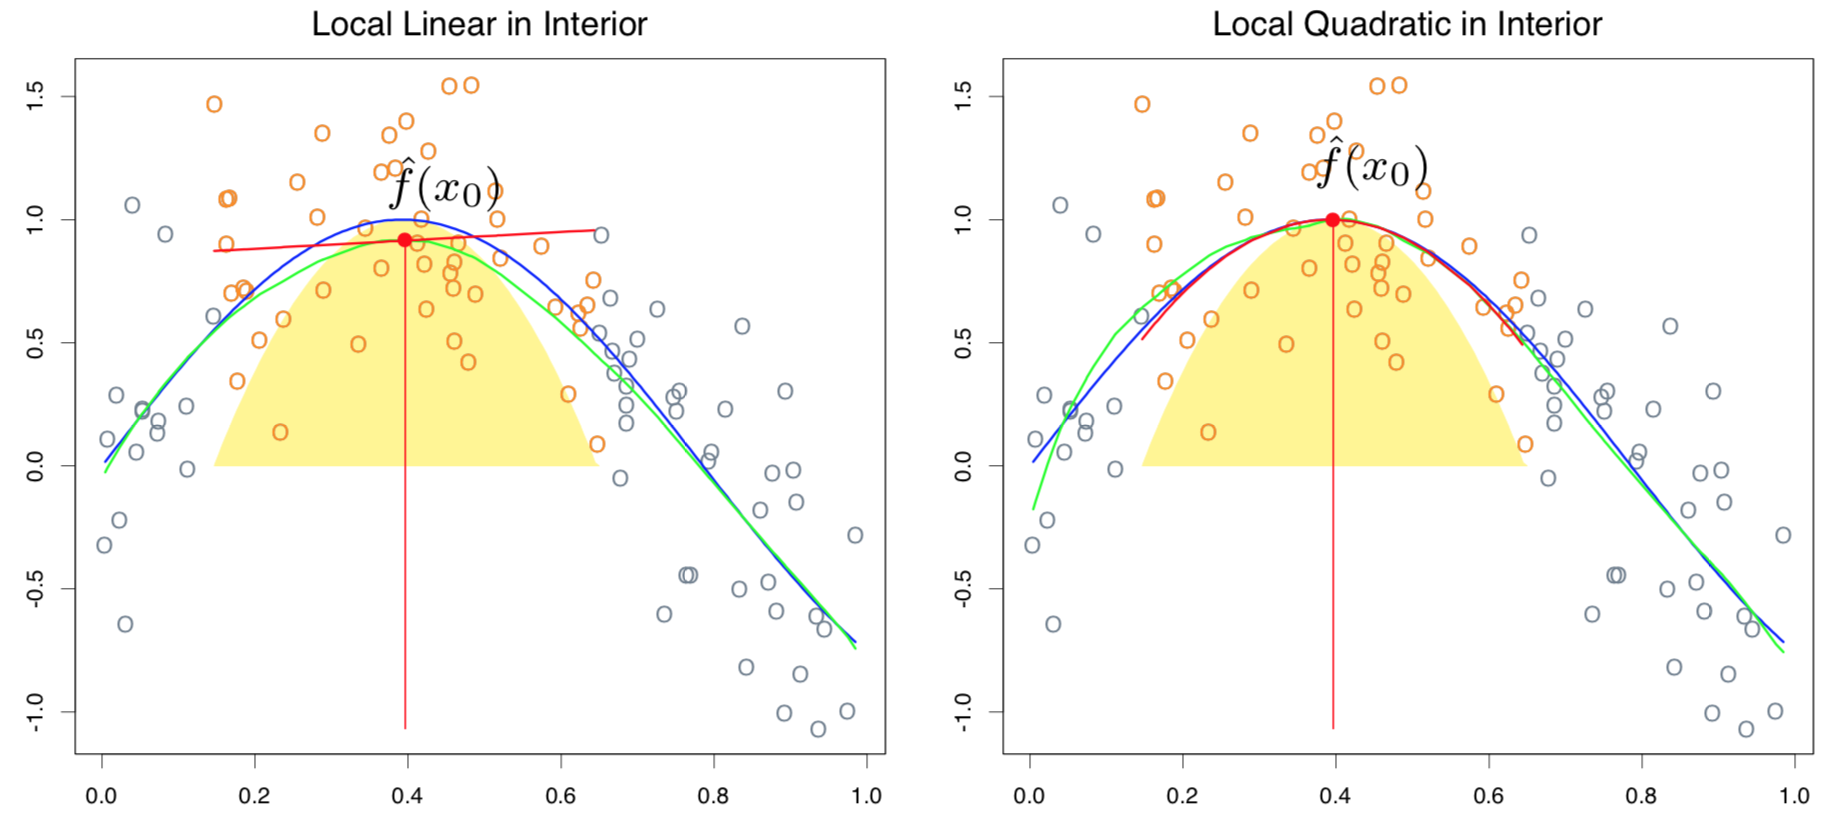
\includegraphics[scale=0.4]{img/localLinQuad}
\caption{Local linear fits exhibit bias in regions of curvature of the true function. Local quadratic fits tend to eliminate this bias.}
\label{localLinQuad}
\end{figure}
Summarizing, local linear fits can help bias dramatically at the boundaries at a modest cost in variance. Local quadratic fits do little at the boundaries for bias, but increase the variance a lot. Local quadratic fits tend to be most helpful in reducing bias due to curvature in the interior of the domain. Asymptotic analysis suggest that local polynomials of odd degree dominate those of even degree. This is largely due to the fact that asymptotically the MSE is dominated by boundary effects.
\subsection{Local regression in $\CMcal{R}^p$}
Let $b(X)$ be a vector of polynomial terms in $X$ of maximum degree $d$. For example, with $d = 1$ and $p = 2$ we get $b(X) = (1,X_1,X_2)$; with $d = 2$ we get $b(X) = (1, X_1, X2, X_1^2, X_2^2, X_1X_2)$; and trivially with $d = 0$ we get $b(X) = 1$. At each $x_0 \in \CMcal{R}^p$ solve:
\begin{equation}
min_{\beta(x_0)} \sum_{i=1}^N K_\lambda (x_0, x_1)\left(y_i - b(x_i)^T\beta\left(x_0\right)\right)^2
\end{equation}
to produce the fit
\begin{equation}
\hat{f} (x_0) = b(x_0)^T\hat{\beta}(x_0)
\end{equation}
While boundary effects are a problem in one-dimensional smoothing, they are a much bigger problem in two or higher dimensions, since the fraction of points on the boundary is larger. In fact, one of the manifestations of the curse of dimensionality is that the fraction of points close to the boundary increases to one as the dimension grows. Directly modifying the kernel to accommodate two-dimensional boundaries becomes very messy, especially for irregular boundaries.  Directly modifying the kernel to accommodate two-dimensional boundaries becomes very messy, especially for irregular boundaries.
Local regression becomes less useful in dimensions much larger than $2$.

For high dimensionality it is impossible to simultaneously maintain localness (i.e., low bias) and a sizable sample in the neighbourhood (low variance) as dimensions increase, without the total sample size increasing exponentially with $p$.

\subsection{Structured local regression models in $\CMcal{R}^p$}
When the dimension to sample-size ratio is unfavorable, local regression does not help us much, unless we are willing to make some structural assumptions about the model.

\subsubsection{Structured kernels}
The default spherical kernel gives equal weight to each coordinate and we can standardize the variables to unit deviation.

Another way is to use a positive definite matrix $A$ to weigh the different coordinates:
\begin{equation}
K_\lambda(x_0, x) = D\left( \frac{(x-x_0)^T\mathbf{A}(x-x_0)}{\lambda}\right)
\end{equation}
Entire coordinates or directions can be downgraded or omitted by imposing appropriate restrictions on $\mathbf{A}$. For example, if $\mathbf{A}$ is diagonal, then we can increase or decrease the influence of individual predictors $X_j$ by increasing or decreasing $A_{jj}$.

\subsubsection{Structured regression function}
We are trying to fit a regression function $\E[Y|X] =f(X_1,X_2, \cdots, X_p)$ in $CMcal{R}^p$ in which every level of interaction is potentially present. It is natural to consider analysis-of-variance (ANOVA) decompositions of the form
\begin{equation}
f(X_1,X_2,\cdots, X_p) = \alpha + \sum_j g_j(X_j) +  \sum_{k<l} g_{kl}(X_k, X_\ell) + \cdots 
\end{equation}
and then introduce structure by eliminating the higher-order terms. Additive models assume only main effect terms: $f(X) = \alpha + \sum_{j=1}^p g_j(X_j)$, second order models will have terms with interactions of order at most two and so on.  The important detail is that at any stage, one-dimensional local regression is all that is needed. The same ideas can be used to fit low-dimensional ANOVA decompositions.

\subsection{Local likelihood and other models}
Any parametric model can be made local.

For example we can use likelihood local to $x_0$,  with the parameters $\theta(x_0) = x_0^T\beta(x_0)$:
\begin{equation}
l\br{\beta(x_0)} = \sum_{i=1}^N K_\lambda (x_0,x_i) l\br{y_i, x_i^T\beta(x_0)}
\end{equation}

Also time-series can be made local by fitting by local least squares with a kernel in order to vary according to the short-term history of the series.
\subsubsection{Local multiclassifier linear logistic regression}
Consider categorical responses $g_i \in {1,2,\cdots, J}$. The global linear model is:
\begin{equation*}
Pr(G=j|X=x) = \frac{e^{\beta_{j0}+\beta_j^Tx}}{1+\sum_{k=1}^{J-1}e^{\beta_{k0}+\beta_k^Tx}}
\end{equation*}
The local log-likelihood for the class $J$ can be written as:
\begin{equation}
\begin{aligned}
&\sum_{i=1}^N K_\lambda(x_0, x_i) \Bigg\{\beta_{g_i0}(x_0)+ \beta_{g_i}(x_0)^T(x_i-x_0)+\\
& -\log\left[ 1+\sum_{k=1}^{J-1}e^{\beta_{k0}(x_0)+\beta_k(x_0)^T(x_i-x_0)}\right]\Bigg\}
\end{aligned}
\end{equation}
Notice that $\beta_{J0}=\beta_{J}=0$ i.e., the last class is taken as reference. Also, we have centred the local regression at $x_0$, so that the fitted posterior probabilities at $x_0$ are simply:
\begin{equation}
\hat{Pr}\br{G=j, X=x_0} = \frac{e^{\hat{\beta}_{j0}(x_0)}}{1+\sum_{k=1}^{J-1}e^{\hat{\beta}_{k0}(x_0)}}
\end{equation}

\subsection{Kernel density classification}
One can use nonparametric density estimates for classification in a straightforward fashion using Bayes' theorem:
\begin{equation}
\hat{Pr}(G=k|X=x_0) = \frac{\hat{\pi}_k \hat{f}_k(x_0)}{\sum_{j=1}^J\hat{\pi}_k \hat{f}_j(x_0)}
\end{equation}
with $\hat{f}_j$ being a fitted nonparametric density estimates for each class separately.

\subsection{Naive-Bayes classifier}
It assumes that given a class $G=j$, the features $X_k$ are independent:
\begin{equation}
f_j(X) = \prod_{k=1}^p f_{jk}(X_k)
\end{equation}
While this assumption is generally not true, it does simplify the estimation
dramatically since $f_{jk}$ can be estimated separately using one dimensional kernel density estimates.
Despite these rather optimistic assumptions, Naive-Bayes classifiers often outperform far more sophisticated alternatives. The reasons are that although the individual class density estimates may be biased, this bias might not hurt the posterior probabilities as much, especially near the decision regions. In fact, the problem may be able to withstand considerable bias for the savings in variance such a "naive" assumption earns.

\subsection{Radial basis functions}
Radial basis functions combine the idea of basis methods and kernel functions by treating $K_\lambda(\xi, x)$ as a basis function:
\begin{equation}
f(x) = \sum_{j=1}^M K_{\lambda_j}(\xi_j,x)\beta_j = \sum_{j=1}^M D\br{\frac{\|x-\xi_j\|}{\lambda_j}}\beta_j
\end{equation}
A popular choice for $D$ is the standard Gaussian density function. There are several methods to estimate the parameters, among which one of the most common is the least squares. We can optimize the sum-of-squares with respect to all parameters:
\begin{equation}
\min_{\{\lambda_j, \xi_j, \beta_j\}_1^M} \sum_{i=1}^N\br{y_i -\beta_0 -\sum_{j=1}^M \beta_j e^{-\frac{(x_i-\xi_j)^T(x_i-\xi_j)}{\lambda_j^2}}}^2
\end{equation}
This model is referred to as RBF network, with $\xi_J$ and $\lambda_j$ playing the role of weights. This criterion is non-convex with multiple local minima.

Another way is to estimate $\{\lambda_j,\xi_j\}$ separately from $\beta_j$. Often, the kernel parameters $\lambda_j$ and $\xi_j$ are chosen in an unsupervised way using the $X$ distribution alone. One of the method is to fit a Gaussian mixture density model  to the training $x_i$, which provides both the centres $\xi_j$ and the scales $\lambda_j$. Other approaches use cluster methods to locate $\xi_j$ and treat $\lambda_j=\lambda$ as a hyper-parameter.

Using a constant $\lambda$ might create holes-regions (regions that are not fitted by any gaussian) where no kernels has appreciable support. Renormalized radial basis functions solve this problem:
\begin{equation}
h_j(x) = \frac{D\br{\frac{\|x-\xi_j\|}{\lambda}}}{\sum_{k=1}^MD\br{\frac{\|x-\xi_k\|}{\lambda}}}
\end{equation}

\subsection{Mixture Models for Density Estimation and Classification}
The mixture model can be viewed as a kind of kernel method:
\begin{equation}
\begin{aligned}
&f(x) = \sum_{m=1}^M \alpha_m \phi(x, \mu_m,\Sigma_m)\\
&\sum_m \alpha_m =1
\end{aligned}
\label{mix}
\end{equation}
It is possible to use any density instead of the Gaussian densities.

The parameters are usually fit by maximum likelihood, using the EM algorithm. If the covariance matrix is force to be scalar $\Sigma_m = \sigma_m \I$, then \autoref{mix} has the form of a radial basis expansion. If $\sigma_m = \sigma >0$ and $M \uparrow $

%%%%%%%%%%%%%%%%%%%%%%%%%%%%%%%%%%%%%%%%%%%%%%%%%%%%%%%%%%
%%%%%%%%------------------------------NEW SECTION------------------------------%%%%%%%%%
%%%%%%%%%%%%%%%%%%%%%%%%%%%%%%%%%%%%%%%%%%%%%%%%%%%%%%%%%%
\newpage
\section{Model assessment and selection}
\textit{Take a look also at this: https://machinelearningmastery.com/probabilistic-model-selection-measures/}
\begin{definition}{\textbf{Training error}}: it is the average loss over the training samples:
\begin{equation}
\bar{err} = \frac{1}{N}\sum_{i=1}^N L(y_i, \hat{f}(x_i))
\end{equation}

For categorical variables it is:
\begin{equation}
\bar{err}  = -\frac{2}{N} \sum_{i=1}^N \log\hat{p}_k(x_i)
\end{equation}
The "$-2$" in the definition makes the log-likelihood loss for the Gaussian distribution match squared-error loss.
\label{trainErr}
\end{definition}

\begin{definition}{\textbf{Test error:}} with  the term \textit{test error} or \textit{generalization error} we indicate the prediction error over an independent test sample different from the one used for the training and it is indicated as 
\begin{equation}
Err_\tau \left[L(Y,\hat{f}(X)|\tau\right]
\end{equation}
where $\tau$ indicates the training set and $X$ and $Y$ are drawn randomly from their joint distribution.
\end{definition}

\begin{definition}{\textbf{Expected prediction error}}: or \textbf{expected test error} is the expectation of the test.
\begin{equation}
Err = \E\left[ L(Y,\hat{f}(X))\right] =  \E\left[Err_\tau\right]
\end{equation}
\end{definition}

\autoref{testErr} shows the prediction errors of the same type of model trained with different training sets in light red and their expectation (average) in dark red.

\begin{figure}
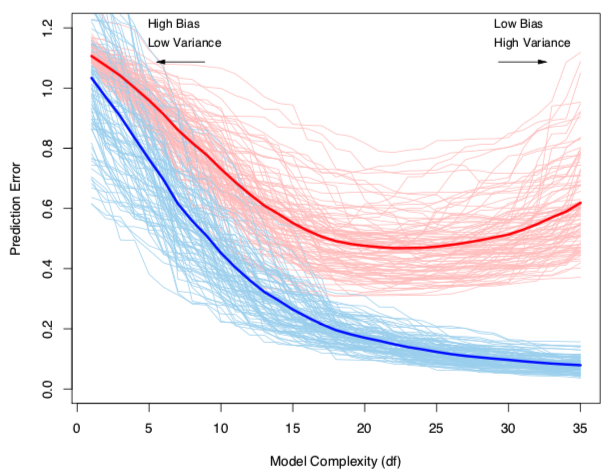
\includegraphics[scale=0.6]{img/testErr}
\caption{Behaviour of test sample and training sample error as the model complexity is varied. The light blue curves show the training error $\bar{err}$, while the light red curves show the conditional test error $Err_\tau$ for $100$ training sets of size $50$ each, as the model complexity is increased. The solid curves show the expected test error $Err$ and the expected training error $E[\bar{err}]$.}
\label{testErr}
\end{figure}
To judge the prediction capability of a model we need to estimate $Err_\tau$. As the model becomes more and more complex, it uses the training data more and is able to adapt to more complicated underlying structures. Hence there is a decrease in bias but an increase in variance. There is some intermediate model complexity that gives minimum expected test error. The training error is not reliable because it always decreases with the model complexity and with too much complexity it looses the capability to generalize.

The same holds for categorical variables (introduced in \autoref{trainErr}). Typical loss functions are:
\begin{equation}
\begin{aligned}
&L(G, \hat{G}) = I(G\ne\hat{G}(X)) \quad\quad \textit{0-1 loss},\\
&L(G, \hat{p}(X)) = -2\sum_{k=1}^K I(G=k)\log\hat{p}_k(X) \quad\quad \textit{-2 $\times$ log-likelihood},\\
\end{aligned}
\end{equation}
where the quantity $-2 \times \log-likelihood$ is generally referred as deviance. The "$-2$", as already said, in the definition makes the log-likelihood loss for the Gaussian distribution match squared-error loss.
A number of methods for estimating the expected test error for a model exists. Typically our model will have a tuning parameter or parameters $\alpha$ and so we can write our predictions as$ \hat{f}(x)_\alpha$
The tuning parameter varies the complexity of our model, and we wish to find the value of $\alpha$ that minimizes error, that is, produces the minimum of the average test error curve. There are two goals that one might want to achieve:
\begin{definition}{\textbf{model selection}}: estimating the performance of different models in order to choose the best one.
\end{definition}
\begin{definition}{\textbf{model assessment}}: having chosen a final model, estimate its prediction error on new data.
\end{definition}


If we are in a data-rich situation, the best approach for both problems is to randomly divide the dataset into three parts: a training set, a validation set, and a test set. The training set is used to fit the models; the validation set is used to estimate prediction error for model selection; the test set is used for assessment of the generalization error of the final chosen model. Ideally, the test set should be kept in a "vault", and be brought out only at the end of the data analysis. It is difficult to give a general rule on how to choose the number of observations in each of the three parts, as this depends on the signal-to- noise ratio in the data and the training sample size. A typical split might be 50\% for training, and 25\% each for validation and testing.

The following methods allows to work in a situation with insufficient data. The methods can be distinguished in analytical (AIC, BIC, MDL, SRM) or by efficiently sample re-use (cross-validation and boot-strap). 
Typically the more complex we make the model $f$, the lower the (squared) bias but the higher the variance.
\subsection{Optimism of the training error rate}
Given a training set $\tau$ the generalization error of a model is:
\begin{equation}
Err_\tau = \E_{X^0, Y^0}\left[ L(Y^0, \hat{f}(X^0))|tau\right]
\end{equation}
where the point $(X^0, Y^0)$ is a new test data point. Averaging over training sets $\tau$ (i.e., averaging over the same type of models $\hat{f}$ but trained with different trainsets belonging to the same distribution):
\begin{equation}
Err = \E_\tau \E_{X^0, Y^0}\left[ L(Y^0, \hat{f}(X^0))|tau\right]
\end{equation}
The training error $\bar{err} = \frac{1}{N}\sum_{i=1}^N L(y_i, \hat{f}(x_i))$  will be less than the true error, because the same data is being used to fit the method and assess its error. A fitting method typically adapts to the training data, and hence the apparent or training error $\bar{err}$ will be an overly optimistic estimate of the generalization error $Err_\tau$, which can be thought as \textit{extra-sample error}. 

The nature of the optimism in the training error can be explained considering the \textit{in-sample error}:
\begin{equation}
Err_{in} = \frac{1}{N} \sum_{i=1}^N E_{Y^0}\left[ L(Y_i^0, \hat{f}(x_i))|\tau\right]
\end{equation}
To explain it better consider the same input points $x_i, \quad i=1,\cdots, N$. In the training set for these points we got a given set of values, while on new data we get a slightly different values $Y^0$ due to the random process involved (for example the noise considering the additive model). The model $\hat{f}$ have been trained using the training set, so for its prediction for those points will be close to the values seen in the training set (influenced by randomness) and it cannot foresee the non-deterministic part in the new samples. We define the optimism as the difference between the real $Err_{in}$ and the training error:
\begin{equation}
op \equiv Err_in - \bar{err}
\end{equation} 
and this is typically positive since the second term is generally biased downward. Averaging the optimism:
\begin{equation}
\omega = \E_y(op)
\end{equation}
where the notation $\E_y$ has been used instead of $\E_\tau$ because the predictors (the inputs) are fixed, while the outputs vary.

For squared error, 0-1 loss functions and other loss functions one can show:
\begin{equation}
\omega = \frac{2}{N} \sum_{i=1}^N Cov(\hat{y_i}, y_i)
\end{equation}
Thus the amount by which err underestimates the true error depends on how strongly $y_i$ affects its own prediction. The harder we fit the data, the greater the covariance will be, thereby increasing the optimism. We have the relationship:
\begin{equation}
\E_y (Err_{in}) = \E_y(\bar{err}) +\frac{2}{N} \sum_{i=1}^N Cov(\hat{y_i}, y_i)
\end{equation}
This expression simplifies if $\hat{y}_i$ is obtained by a linear fit with d inputs or basis functions. For example for the additive model $Y=f(X) + \epsilon$:
\begin{equation}
 \sum_{i=1}^N Cov(\hat{y_i}, y_i) = d\sigma_\epsilon^2
\end{equation}
and so
\begin{equation}
\E_y (Err_{in}) = \E_y(\bar{err}) +\frac{2d}{N} \sigma_\epsilon^2
\label{paramSel}
\end{equation}
We can use these expressions to select the effective number of parameters. The optimism increases with the number $d$ of inputs or basis functions we use, but decreases as the training sample size increases

An obvious way to estimate prediction error is to estimate the optimism and then add it to the training error. The methods such as Cp, AIC, BIC and others work in this way, for a special class of estimates that are linear in their parameters.
In contrast, cross-validation and bootstrap methods are direct estimates of the extra-sample error. These general tools can be used with any loss function, and with nonlinear, adaptive fitting techniques.
In-sample error is not usually of direct interest since future values of the features are not likely to coincide with their training set values. But for comparison between models, in-sample error is convenient and often leads to effective model selection. The reason is that the relative (rather than absolute) size of the error is what matters.

\subsection{$C_p$ metric}
One can estimate the in-sample error as
\begin{equation}
\hat{Err} = \bar{err}+\hat{\omega}
\end{equation}
where $\hat{\omega}$ is an estimate of the average optimism. Using \autoref{paramSel}:
\begin{equation}
C_p = \bar{err} +\frac{2d}{N} \hat{\sigma}_\epsilon^2
\end{equation}
where $\hat{\sigma}_\epsilon^2$ is an estimate of the noise variance.

The model with lowest $C_p$ should be selected.

\subsection{Akaike Information Criterion}
Suppose we have models $\CMcal{M}_1, \cdots, \CMcal{M}_k$ where each model is a set of densities:
\begin{equation}
\CMcal{M}_j = \left\lbrace p(y;\theta_j):\theta_j \in \Theta_j\right\rbrace.
\end{equation}
and we have data $Y_1,\cdots, Y_n$ drawn from an unknown density $f$ that we do not know if it is in any of the models. Let $\hat{\theta}_j$ be the Maximum Likelihood estimation from the model $j$. Using this we can estimate $f$ with $\hat{p}_j(y) = p(y, \hat{\theta}_j)$. The quality of $\hat{p}_j(y)$ (i.e., its distance form $f$) can be measured by the \textbf{Kullback-Leibler distance}:
\begin{equation}
\begin{aligned}
K(p, \hat{p}_j) &= \int p(y) \log \frac{p(y)}{\hat{p}_j(y)} dy = \\
&=\int p(y) \log p(y) dy  - \int p(y) \log \hat{p}_j(y) dy 
\end{aligned}
\end{equation}
We want to minimize this distance. The first term is constant while we can act on $ \hat{p}_j(y)$. Since it is a probability (i.e.  $\hat{p}_j(y)$ is at most one, minimizing the distance is equivalent to maximizing the second term:
\begin{equation}
K_j = \int p(y) \log \hat{p}_j(y) dy 
\end{equation}
Intuitively one estimate of $K_j$ might be:
\begin{equation}
\bar{K}_j = \frac{1}{N} \sum_{i=1}^N \log p_j(Y_i,\hat{\theta}_j)  = \frac{\ell_j(\hat{\theta_j})}{N} 
\end{equation}
i.e., assuming a uniform distribution. This estimation is very biased because data are being used twice: once for the MLE and the second one to calculate the integral. So we have $\bar{K}_j \ne K_j$. We want to find such difference.

Let us drop the index $j$ (i.e., we are considering just one model and not a set) and just use $K$ and $\bar{K}$. Let $\theta_0$ be the parameters that minimize $K(f,p(\cdot, \theta))$. So $p(y, \theta_0)$ is the closest density in the model to the true density. Let $\ell(y,\theta)=\log p (y, \theta)$ and let us define the \textbf{score} as:
\begin{equation}
s(y,\theta) = \frac{\partial \log p (y, \theta)}{\partial \theta}
\end{equation}
and let $H(y, \theta)$ be the matrix of second derivatives.
Let
\begin{equation}
Z_N = \sqrt{N}\br{\hat{\theta} - \theta_0}
\end{equation}
and recall (?) that :
\begin{equation}
Z_N \rightarrow \CMcal{N}(0, J^{-1}VJ^{-1})
\end{equation}
where 
\begin{equation}
\begin{aligned}
&J = -\E\left[ H(Y,\theta_0\right]\\
& V = Var(s(Y,\theta_0))
\end{aligned}
\end{equation}
Let 
\begin{equation}
S_N = \frac{1}{N}\sum_{i=1}^N s(Y_i, \theta_0)
\end{equation}
By the \textbf{Central Limit Theorem}, and recalling that $\theta_0$ is the value that minimizes $K$ (if it is a convex function then for this value the score is $0$ i.e., $0$ mean):
\begin{equation}
\sqrt{N}S_N \rightarrow \CMcal{N}(0, V)
\end{equation}
since 
\begin{equation}
\begin{aligned}
\Var\left[ \sqrt{N} S_n\right] &= \E\left[ \br{\sqrt{N} S_n - \cancel{\mu_{S_n}}}^2\right]= \\
&= N \E\left[ \br{\frac{1}{N}\sum_{i=1}^N s(Y_i, \theta_0)}^2\right] = \frac{1}{N} \E\left[ \br{\sum_{i=1}^N s(Y_i, \theta_0)}^2\right] =\\
&= \frac{1}{N}  \br{\sum_{i=1}^N \E\left[s(Y_i, \theta_0)\right]^2} =\frac{1}{N} NV=V
\end{aligned}
\end{equation}
Now $J$ is a scalar, considering the distribution $JZ_N$ where $Z_N \rightarrow\CMcal{N}(0, J^{-1}VJ^{-1})$, the result is still a distribution with $0$. For the variance let us use the property:
\begin{equation}
\begin{aligned}
&\Var\left[ JZ_N\right] = J(J^{-1}VJ^{-1})J^T = V\\
&\Rightarrow JZ_N \sim \CMcal{N}(0,V)
\end{aligned}
\label{varMul}
\end{equation}

By using \textbf{Taylor series expansion}:
\begin{equation}
K \approx \int p(y) \br{\log p(y, \theta_0) + \cancel{\br{\hat{\theta} - \theta_0}^Ts(y,\theta_0)}+\frac{1}{2}\br{\hat{\theta} - \theta_0}^TH(y,\theta_0)\br{\hat{\theta} - \theta_0}} dy
\end{equation}
The second term $\br{\hat{\theta} - \theta_0}^Ts(y,\theta_0)$ is $0$ because the score has $0$ mean. Defining 
\begin{equation}
K_0  = \int  p(y) \log p(y, \theta_0)dy
\end{equation}
we have:
\begin{equation}
\begin{aligned}
K &\approx K_0 + \frac{1}{\sqrt{N}}Z_N^T \int H(y,\theta_0) p(y) dy \frac{1}{\sqrt{N}}Z_N  = \\
& =K_0 + \frac{1}{\sqrt{N}}Z_N^T \int H(y,\theta_0) p(y) dy \frac{1}{\sqrt{N}}Z_N = k_0 -\frac{1}{2N} Z_N^TJZ_N
\end{aligned}
\end{equation}
Now applying the \textbf{Taylor series expansion} to $hat{K}$:
\begin{equation}
\bar{K}  \approx \frac{1}{N} \sum_{i=1}^N \br{\ell(Y_i,\theta_0) + \br{\hat{\theta} - \theta_0}^Ts(Y_i,\theta_0)} + \frac{1}{2}\br{\hat{\theta} - \theta_0}^TH(Y_i,\theta_0)\br{\hat{\theta} - \theta_0}
\end{equation}
Defining 
\begin{equation}
\begin{aligned}
&A_N = \frac{1}{N} \sum_{i=1}^N \ell(Y_i, \theta_0) - K_0 = \frac{1}{N} \sum_{i=1}^N \br{\ell(Y_i, \theta_0) - K_0}\\
&J_N = -\frac{1}{N} \sum_{i=1}^NH(Y_i,\theta_0) - \xrightarrow{P} J
\end{aligned}
\end{equation}
we have
\begin{equation}
\begin{aligned}
\bar{K} &\approx K_0 + A_N + (\hat{\theta} - \theta_0)S_N -\frac{1}{2N} Z_N^TJ_NZ_N \approx\\
&\approx K_0 + A_N + \frac{Z_N^T}{N}\sqrt{N}J^{-1}JS_N -\frac{1}{2N} Z_N^TJZ_N  = \\
&= K_0 + A_N + \frac{Z_N^TJZ_N}{N} -\frac{1}{2N} Z_N^TJZ_N
\end{aligned}
\end{equation}
where $\autoref{varMul}$ has been used again ($J^{-1}S_N \rightarrow J^{-1}\CMcal{N}(0,V)= \CMcal{N}(0,J^{-1}VJ^{-1}) = Z_N$).
We need another property. Let $\epsilon$ be a random vector with mean $\mu$ and variance $\Sigma$ and let
\begin{equation}
Q = \epsilon^T A \epsilon
\end{equation} 
with $Q$ called a quadratic form. Then
\begin{equation}
\E\left[ Q\right] = trace(A\Sigma)+\mu^TA\mu
\end{equation}
Now taking the difference:
\begin{equation}
\begin{aligned}
\E\left[hat{K}-K\right] &= \E\left[A_N\right]+\E\left[ \frac{Z_N^TJZ_N}{N}\right] = 0 + \frac{trace(J J^{-1}VJ^{-1})}{N}=\\
& \frac{trace(J^{-1}VJ^{-1}J)}{N}= \frac{trace(J^{-1}V)}{N} 
\end{aligned}
\end{equation}
If the model is correct then $J^{-1}=V$ so that $trace(J^{-1}V)= trace(I)=d$:
\begin{equation}
K \approx\hat{K} =  \bar{K} -\frac{d}{N}
\end{equation}
So the bias is approximately $\frac{d}{N}$.
Considering the model $j$:
\begin{equation}
\begin{aligned}
\hat{K}_j &= \bar{K}_j -\frac{d_j}{N}\\
AIC(j) &= 2N \hat{K}_j = \ell_j(\hat{\theta}_j) -2d_j
\end{aligned}
\end{equation}
Maximizing $\hat{K}_j$ is the same as maximising $AIC(j)$. Constants are not important in the maximization process. With this representation we choose the model with the highest AIC.
Other books use the following representation:
\begin{equation}
\begin{aligned}
AIC(j) =-\frac{2}{N}\ell_j(\hat{\theta}_j) +2\frac{d_j}{N}\\
\end{aligned}
\end{equation}
and with this representation the best model is the one that minimizes the AIC, since the signs have been inverted.

For the Gaussian model, with variance $\sigma^2_\epsilon = \hat{\sigma}^2_\epsilon$, the AIC statistic is equivalent to $C_p$.

For non-linear and other complex models we replace $d$ with a measure of the model complexity. Given a set of models $f_\alpha$, $\bar{err}(\alpha)$ is the training error and $d(\alpha)$ the number of parameters:
\begin{equation}
AIC(\alpha) = \bar{err}(\alpha) + 2\frac{d\alpha}{N}\hat{\sigma}^2_\epsilon.
\end{equation}
\subsection{Effective number of parameters}
A linear fitting method (linear regression, derived basis sets and smoothing methods with quadratic shrinkage such as ridge regression and cubic smoothing splines) have the form:
\begin{equation}
\hat{\y} = \mathbf{S}\y
\end{equation}
where $\mathbf{S}$ is a $N\times N$ matrix. The effective number of parameters is defined as:
\begin{equation}
df(\mathbf{S}) = trace(\mathbf{S}) = M
\end{equation}
since $\mathbf{S}$ is an orthogonal projection matrix onto a basis set spanned by $M$ features. Then instead of $d$ we use $trace(\mathbf{S})$.

For models like NN in which we minimize an error function with weight decay penalty (regularization) $\alpha \sum_m w_m^2$, the effective number of parameters has ethe form:
\begin{equation}
df(\alpha) = \sum_{m=1}^M \frac{\theta_m}{\theta_m+\alpha}
\end{equation}
where $\theta_m$ are the eigenvalues of the Hessian matrix $\partial R(\omega) /\partial \omega\partial \omega^T$.

\subsection{Bayesian Information Criterion}
Known also as \textit{Schwarz Criterion}, it is equivalent to the MDL. We choose $j$ to maximize
\begin{equation}
BIC(j) = \ell_j(\hat{\theta}_j) - \frac{d_j}{2}\log n
\end{equation}
It is similar to the AIC but it has a stronger penalization and tends to choose simpler models.

Using priors $\pi_j(\theta_j)$ on the parameters $\theta_j$ and a probability $p_j$ indicating the probability that  $\CMcal{M}_j$ is the true model, by Bayesian theory, indicating with $\mathbf{Z}$ the training set, we have:
\begin{equation}
P(\CMcal{M}_j|\mathbf{Z}) \propto p(\mathbf{Z}|\CMcal{M}_j) p_j
\end{equation}
Furthermore
\begin{equation}
\begin{aligned}
p(\mathbf{Z}|\CMcal{M}_j) &= \int p(\mathbf{Z}|\CMcal{M}_j,\theta_j)\pi_j(\theta_j) d\theta_j = \\
&=\int L(\theta_j)\pi_j(\theta_j) d\theta_j
\end{aligned}
\end{equation}
So equivalently we choose $j$ to maximize:
\begin{equation}
\log \int L(\theta_j)\pi_j(\theta_j) d\theta_j + \log p_j
\end{equation}
Using Taylor expansion:
\begin{equation}
\begin{aligned}
\log \int L(\theta_j)\pi_j(\theta_j) d\theta_j + \log p_j &\approx \ell_j(\hat{\theta}_j) - \frac{d_j}{2}\log n \\
\Rightarrow BIC(j) &= \ell_j(\hat{\theta}_j) - \frac{d_j}{2}\log n
\end{aligned}
\label{BIC}
\end{equation}
The prior has been ignored because it can be shown that the terms involving the prior are lower orders than the ones appearing in \autoref{BIC}. Again in some books the signs are inverted.

\textbf{The difference from AIC and Cross-Validation} is that BIC assumes that one of the models is true and that we are trying to find the model most likely to be true in a Bayesian sense. AIC and Cross-Validation tries to find the model that predicts the best.

Under the Gaussian model, assuming the variance $\sigma_\epsilon^2$ is known, with a squared error loss:
\begin{equation}
\begin{aligned}
\bar{err} &=  \sum_i\br{y_i - \hat{f}(x_i)}^2\\
2 \ell_j(\hat{\theta}_j) &= -N\frac{\bar{err}}{\sigma_\epsilon^2}\\
BIC(j) &= -\frac{N}{2\sigma_\epsilon^2}\bar{err} - \frac{d_j}{2}\log n = \frac{N}{2\sigma_\epsilon^2} \left[ \frac{d_j}{N} \sigma_\epsilon^2 \log N - \bar{err} \right]
\end{aligned}
\end{equation}
Hence BIC is proportional to AIC with the factor 2 replaced by $\log N$.

\subsection{Minimum Description Length}
The minimum description length (MDL) principle is a formalization of Occam's razor in which the best hypothesis (a model and its parameters) for a given set of data is the one that leads to the best compression of the data.
The Minimum Description Length is the minimum number of bits, or the minimum of the sum of the number of bits required to represent the data and the model.
$\cdots$

\subsection{Cross-Validation}
It is the simplest and most widely used widely used method for estimating prediction error is cross-validation. This method directly estimates the expected extra-sample error. It consists of dividing data set  in parts: a training set and using an independent test sample from the joint distribution. So one set is used for training and the other to avoid overfitting (to validate the model).

\subsubsection{K-fold cross-validation}
K-fold cross-validation uses part of the available data to fit the model, and a different part to test it.
For the $k-th$ part, we fit the model using the other $K-1$ parts for training and we calculate the prediction error of the fitted model on the $k-th$ part. We do this for all $k=1,\cdots, K$, fitting the model resulting from the previous step using the new partition of data.
Typical choices of $K$ are $5$ or $10$. $K=N$ case is known as live-one-out cross-validation. The higher value of $K$ leads to less biased model (but large variance might lead to overfit), where as the lower value of $K$ is similar to the train-test split approach we saw before.

\subsubsection{Cross validation according to "Hands on Machine Learning"}
Generally a model can be evaluated using a training set and a test set. When one has to choose a hyperparameter a \textbf{validation set} of data is used. Models with different parameters are trained using the training set, the model and hyperparameters that perform best according to the validation test are selected and one is satisfied by the performances, finally run a single test on the test set. 

When evaluating the hyperparameter on the test-set directly, the problem is that the test-set is being used multiple times: to select the hyperparameters and to finally evaluate the model. The hyperparameters were chosen for this specific test-set so it is clear the error on this specific set is reduced.

This however requires lots of data. To avoid this cross validation is used:  the training set is split into complementary subsets, and each model is trained against a different combination of these subsets and validated against the remaining parts. Once the model type and hyperparameters have been selected, a final model is trained using these hyperparameters on the full training set, and the generalized error is measured on the test set.

\subsection{Bootstrap Methods}
The general idea  is to randomly draw datasets with replacement from training data. Samples are constructed by drawing observations from a large data sample one at a time and returning them to the data sample after they have been chosen. This allows a given observation to be included in a given small sample more than once. This approach to sampling is called sampling with replacement. This is done $B$ times, producing $B$ datasets.

For the process we need to decide the number of bootstrap samples and a sample size. Then for each boostrap sample, we refit the model to each of the bootstrap datasets and examine the behaviour of the fits over the $B$ replications.

[From wiki:]
As an example, assume we are interested in the average (or mean) height of people worldwide. We cannot measure all the people in the global population, so instead we sample only a tiny part of it, and measure that. Assume the sample is of size N; that is, we measure the heights of N individuals. From that single sample, only one estimate of the mean can be obtained. In order to reason about the population, we need some sense of the variability of the mean that we have computed. The simplest bootstrap method involves taking the original data set of N heights, and, using a computer, sampling from it to form a new sample (called a 'resample' or bootstrap sample) that is also of size N. The bootstrap sample is taken from the original by using sampling with replacement (e.g. we might 'resample' 5 times from [1,2,3,4,5] and get [2,5,4,4,1]), so, assuming N is sufficiently large, for all practical purposes there is virtually zero probability that it will be identical to the original "real" sample. This process is repeated a large number of times (typically 1,000 or 10,000 times), and for each of these bootstrap samples we compute its mean (each of these are called bootstrap estimates). We now can create a histogram of bootstrap means. This histogram provides an estimate of the shape of the distribution of the sample mean from which we can answer questions about how much the mean varies across samples.

%%%%%%%%%%%%%%%%%%%%%%%%%%%%%%%%%%%%%%%%%%%%%%%%%%%%%%%%%%
%%%%%%%%------------------------------NEW SECTION------------------------------%%%%%%%%%
%%%%%%%%%%%%%%%%%%%%%%%%%%%%%%%%%%%%%%%%%%%%%%%%%%%%%%%%%%
\newpage
\section{Additive models}
A linear model has the form $\alpha + f_1(X_1) + f_2(X_2) + f_3(X_3) + \cdots$, where $X$ are the predictors.

\subsection{Tree based methods}
Tree-based methods partition the feature space into a set of rectangles, and then fit a simple model (like a constant) in each one.

We restrict attention to recursive binary partitions. We first split the space into two regions, and model the response by the mean of $Y$ in each region. We choose the variable and split-point to achieve the best fit. Then one or both of these regions are split into two more regions, and this process is continued, until some stopping rule is applied.

For example we first split at $X_1 = t_1$. Then the region $X_1 \le t_1$ is split at $X_2 =t_2$ and the region $X_1 >t_1$ is split at $X_1 =t_3$ and so on. To each sub-region we assign a constant as output:
\begin{equation}
\hat{f}(X) = \sum_{m=1}^M c_m I\{(\x \in \CMcal{R}_m\}
\end{equation}
An advantage of this representation is its interpretability. When more than 2 inputs are involved, it is difficult to represent the partition of the input space. 
\begin{figure}
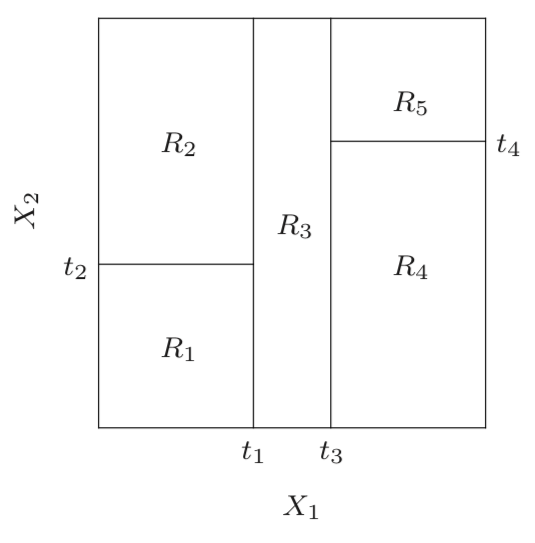
\includegraphics[scale=0.4]{img/tree1}
\caption{2D-input space binary tree partition.}
\label{tree1}
\end{figure}
\begin{figure}
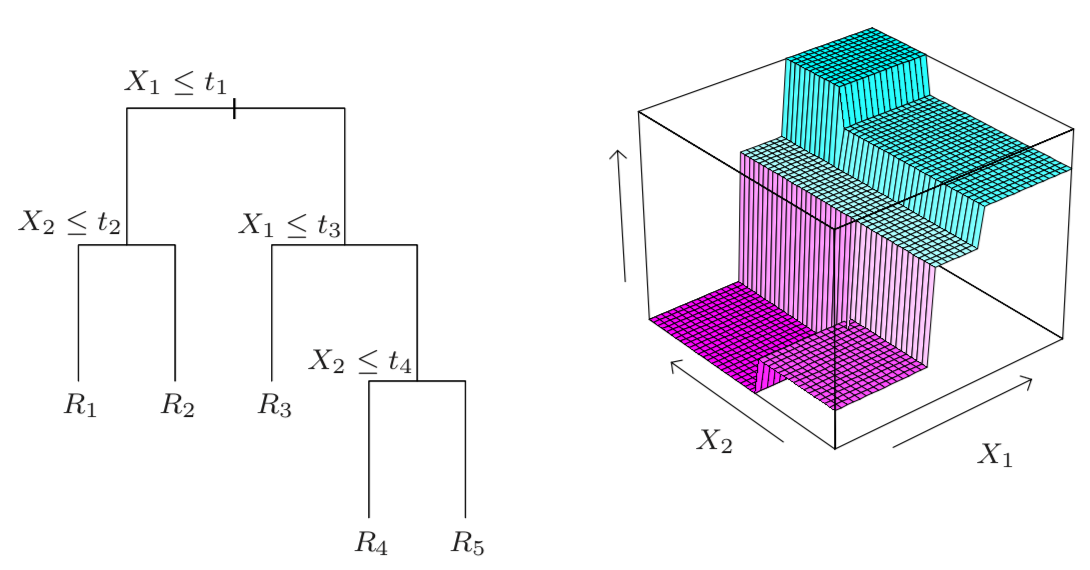
\includegraphics[scale=0.39]{img/tree2}
\caption{Another representation of the binary tree on the left. On the right the 3D resulting shape of the function.}
\label{tree2}
\end{figure}
\subsubsection{Regression Trees}
The algorithm needs to decide automatically the splitting variables and points. We can start defining the values of the constant of each region:
\begin{equation}
\hat{c}_m = ave(y_i|x_i \in \CMcal{R}_m)
\end{equation}
Now finding the best binary partition in terms of minimum sum of squares is generally computationally infeasible. Hence we proceed with a greedy algorithm. Consider a splitting variable $j$ and split point $s$ and define the pair of half-planes:
\begin{equation}
R_1(j,s) = \{X|X_j \le s \}. \quad R_2(j,s) = \{X|X_j > s \}
\end{equation}
Then we seek the splitting variable $j$ and split point $s$ that solve:
\begin{equation}
\begin{aligned}
&\min_{j,s}\left[ \min_{c_1} \sum_{x_i \in \CMcal{R}_1(j,s)}  (y_i-c_1)^2 + \min_{c_2} \sum_{x_i \in \CMcal{R}_2(j,s)}  (y_i-c_2)^2\right]\\
&\hat{c}_1 = ave (y_i|x_i \in R_1(j,s)) \\
&\hat{c}_2 = ave (y_i|x_i \in R_2(j,s)) 
\end{aligned}
\end{equation}
For each splitting variable, the determination of the split point s can be done very quickly and hence by scanning through all of the inputs, determination of the best pair $(j, s)$ is feasible. Having found the best split, we partition the data into the two resulting regions and repeat the splitting process on each of the two regions. Then this process is repeated on all of the resulting regions.


Tree size is a tuning parameter governing the model's complexity, and the optimal tree size should be adaptively chosen from the data. One approach would be to split tree nodes only if the decrease in sum-of-squares due to the split exceeds some threshold. This strategy is too short-sighted, however, since a seemingly worthless split might lead to a very good split below it.
The preferred strategy is to grow a large tree $T_0$, stopping the splitting process only when some minimum node size (say 5) is reached. Then this large tree is pruned using \textbf{cost-complexity pruning}.

The \textbf{cost-complexity pruning} is the following. We define a subtree $T$ of $T_0$. obtained by collapsing any number of its internal nodes. We index the terminal nodes by $m$. let $|T|$ denote the number of terminal nodes in $T$ and 
\begin{equation}
\begin{aligned}
N_m &= \#\{x_i \in \CMcal{R}_m\}\\
\hat{c}_m &= \frac{1}{N_m} \sum_{x_i \ in \CMcal{R}_m} y_i\\
Q_m(T) &= \frac{1}{N_m} \sum_{x_i \in R_m}(y_i - \hat{c}_m)^2
\end{aligned}
\end{equation} 
We define the cost complexity criterion:
\begin{equation}
C_\alpha (T) = \sum_{m=1}^{|T|} N_m Q_m(T) + \alpha |T|
\end{equation}
The idea is to find for each $\alpha$ the subtree $T_\alpha$ of $T_0$ to minimize such a function.
For each $\alpha$ there is a unique smallest subtree $T_\alpha$ that minimizes $C_\alpha(T)$. To find $T_\alpha$ we use the \textbf{weakest link pruning}: we collapse the internal node that produces the smallest per-node increase and we continue umtil we produce the single-node (root) tree. So we have a sequence of subtrees that must contain $T_\alpha$. We choose $\alpha$ to minimize the cross-validated sum of squares, obtaining the tree $T_\alpha$.

\subsection{Classification trees}
The procedure is very similar. In a node $m$ representing the region $R_m$ with $N_m$ observations, let 
\begin{equation}
\hat{p}_{mk} = \frac{1}{N_m}\sum_{\x_i\in R_m} I(y_i=k)
\end{equation}
We classify the observations in node $m$ to class
\begin{equation}
k(m) =argmax_k \hat{p}_{mk},
\end{equation}
the majority class in node $m$. Different measures $Q_m(T)$ of node impurity exist
\begin{equation}
\begin{aligned}
&\textbf{Misclassification error} \quad \frac{1}{N_m} \sum_{i\in \CMcal{R}_m} I(y_i \ne k(m))=1-\hat{p}_{km}\\
&\textbf{Gini index} \quad\quad \sum_{k\ne k'} \hat{p}_{mk}\hat{p}_{mk'} = \sum_{k=1}^K \hat{p}_{mk}(1- \hat{p}_{mk})\\
&\textbf{Cross-entropy or deviance} \quad -\sum_{k=1}^K \hat{p}_{mk}\log \hat{p}_{mk}
\end{aligned}
\end{equation}

These trees are referred as CART (classification and regression trees).
\subsubsection{Linear Combination splits}
Rather than using splits of the type $X_j\le s$ we can use splits of the type $\sum a_j X_j \le s$. The weights $a_j$ and split point $s$ are optimized to minimize the relevant criterion  such as the Gini index.

\subsubsection{Limitations of trees}
One major problem of trees is \textbf{the instability (i.e., high variance)}. A small change in the data can result in a very different series of splits, making interpretation somewhat precarious. The major reason is the hierarchical nature of the process: the effect of an error in the top split is propagated down to all the next splits. The problem can be attenuated but not completely solved.

Another problem of trees is the \textbf{lack of smoothness}. This is not a problem in classification but it is in regression.

Also they are not good at capturing additive structures, such as $Y = c_1 (X_1 < t_1) + c_1 (X_1 < t_1)+\epsilon$ where the noise is $0$ mean. Then a binary tree might make its first split on $X_1$ near $t_1$. At the next level down it would have to split both nodes $X_2$ at $t_2$ in order to capture the additive structure. This is achieved with sufficient data, but it it is a fragile mechanism and can fail in case of many additive effects.
\subsection{Patient rule induction method (PRIM)}
Also PRIM finds boxes in the feature space, but it seeks boxes in which the response average is high. Hence it looks for maxima in the target function, an exercise known as bump hunting. The main box construction method in PRIM works starting with a box containing all of the data. The box is compressed along one face by a small amount, and peeling off a constant portion of data denoted by $\alpha$. Typically $\alpha$ is $0.05$ and $0.1$ of the remaining points at each stage. The face chosen for compression is the one resulting in the largest box mean, after the compression is performed. Then the process is repeated, stopping when the current box contains some minimum number of data points.

After the top-down sequence is computed, PRIM reverses the process, expanding along any edge, if such an expansion increases the box mean. This is called pasting. The result of these steps is a sequence of boxes, with different numbers of observation in each box. Cross-validation, combined with the judgement of the data analyst, is used to choose the optimal box size. Denote by $B_1$ the points in this first box. These points are now removed from the training set and we repeat the two processes (top-down peeling and bottom-up pasting) several times, obtaining for each iteration a new box $B_i$. Each box is defined by a set of rules involving a subset of predictors such as:
\begin{equation}
(a_1 \le X_1 \le b_1) \quad\quad (b_1 \le X_3 \le b_2)
\end{equation}
PRIM can handle a categorical predictor by considering all partitions of the predictor, as in CART. Missing values are also handled in a manner similar to CART. PRIM is designed for regression

\begin{algorithm}[!ht]
Start with all of the training data, and a maximal box containing all of the data;\\

Consider shrinking the box by compressing one face, so as to peel off the proportion $\alpha$ of observations having either the highest values of a predictor $X_j$ or the lowest. Choose the peeling that produces the highest response mean in the remaining box;\\

Repeat step 2 until some minimal number of observations (say 10) remain in the box;\\

Expand the box along any face, as long as the resulting box mean increases;\\

Steps 1-4 give a sequence of boxes, with different numbers of observations in each box. Use cross-validation to choose a member of the sequence. Call the box $B_1$.\\

Remove the data in the box $B_1$ from the dataset and repeat steps 2-5 to obtain a second box. and continue to get as many boxes as desired.
\end{algorithm}

\begin{figure}
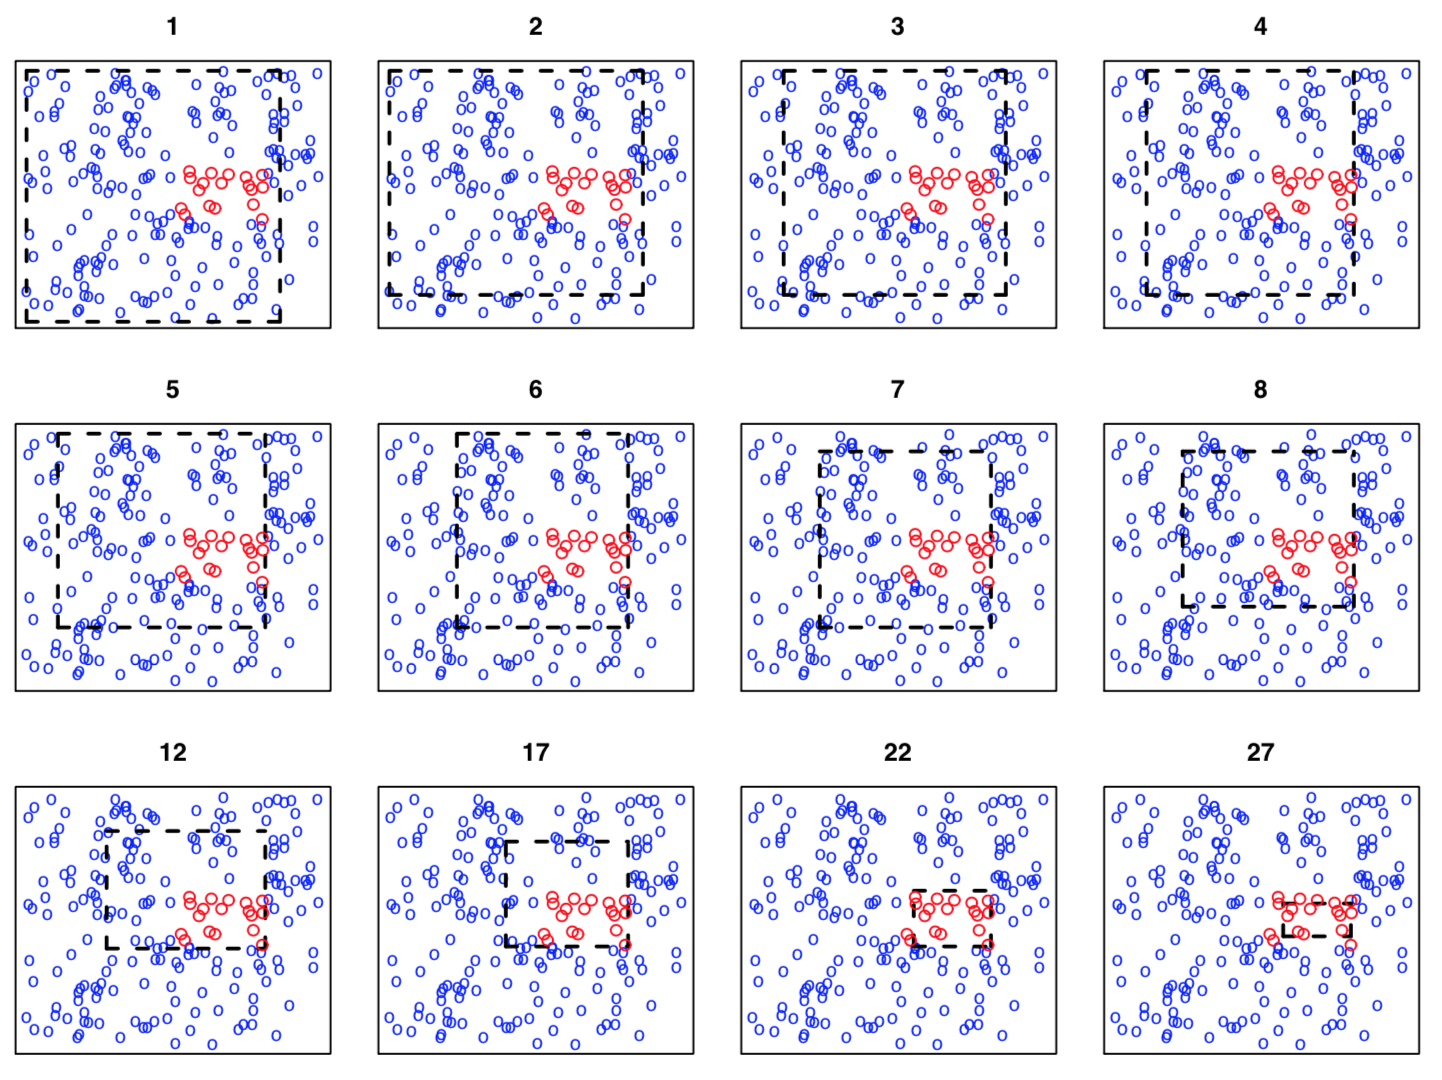
\includegraphics[scale=0.4]{img/PRIM}
\caption{Steps in PRIM.}

\end{figure}
PRIM is designed for binary regression. There is no simple way to deal with $k>2$ classes simultaneously: it is possible to run PRIM separately for each class versus a baseline class.In any case, the ability of PRIM to be more patient should help the top-down greedy algorithm find a better solution.

\subsection{Multivariate Adaptive Regression Splines (MARS)}
It is a procedure well-suited for high-dimensional problems. MARS uses expansions in piecewise linear basis functions of the form $(x-t)_+$ and $(t-x)_+$.

Each function is piecewise linear, with a knot at the value $t_1$. We call the two functions a \textbf{reflected pair}. The idea is to form reflected pairs for each input $X_j$ with knots at each observed value $x_{ij}$ of that input. If all of the input values are distinct, there are $2Np$ basis functions altogether.
The model-building strategy is like a forward stepwise linear regression, but instead of using the original inputs, we are allowed to use functions from the set $\CMcal{C}$ and their products:
\begin{equation}
\CMcal{C} = \{(X_j-t)_+, (t-X_j)_+\}_{t \in \{x_{1j},\cdots, x_{Nj}\}, j=1,\cdots,p}
\end{equation}
Thus the model has the form:
\begin{equation}
f(X) = \beta_0 + \sum_{m=1}^M \beta_m h_m(X)
\end{equation}
where each $h_m(X)$ is a function in $\CMcal{C}$ or a product of two or more such functions. Given the choice for $h_m(X)$, the coefficients are estimated with the residual sum of squares. We start with only a constant $h_0(X)=1$ and all the functions are candidate functions. At each step we consider as a new basis function pair all products of a function $h_m$ in the model set $\CMcal{M}$ with one of the reflected pairs in $\CMcal{C}$. We add to the model $\CMcal{M}$ the term of the form:
\begin{equation}
\hat{\beta}_{M+1}h_\ell(X) (X_j-t)_+ + \hat{\beta}_{M+2}h_\ell(X) (t-X_j)_+, h_\ell \in \CMcal{M}
\end{equation}
that produces the largest decrease in training error. For example, at the first stage we consider adding to the model a function of the form: $\hat{\beta}_1 (X_2-x_{72})_+ + \hat{\beta}_2(x_{72}-X_2)_+$. Then this pair of basis functions is added to the set $\CMcal{M}$ and at the next stage we consider including a pair of products in the form:
\begin{equation}
h_m(X) (X_j-t)_+ \quad\quad \text{and}\quad\quad h_m(X) (t-X_j)_+, t \in \{x{ij}\}
\end{equation}
where for $h_m$ we have the choices:
\begin{equation}
\begin{aligned}
&h_0(X) = 1\\
&h_1(X) = (X_2 - x_{72})_+,  \quad\textit{or}\\
&h_2(X) = (x_{72} - X_2)_+
\end{aligned}
\end{equation}
At the end of this process we have a large model. This model typically overfits the data, and so a backward deletion procedure is applied. The term whose removal causes the smallest increase in residual squared error is deleted from the model at each stage, producing an estimated best model $\hat{f}_\lambda$ of each size (number of terms) $\lambda$. One could use cross-validation to estimate the optimal value of $\lambda$, but for computational savings the MARS procedure instead uses generalized cross-validation:
\begin{equation}
GCV(\lambda) = \frac{\sum_{i=1}^N (y_i - \hat{f}_\lambda(x_i))^2}{(1-\frac{M(\lambda)}{N})^2}
\end{equation}
The value $M(\lambda)$ is the effective number of parameters in the model: this accounts both for the number of terms in the models, plus the number of parameters used in selecting the optimal positions of the knots.

Some mathematical and simulation results suggest that one should pay a price of three parameters for selecting a knot in a piecewise linear regression.
Thus if there are r linearly independent basis functions in the model, and $K$ knots were selected in the forward process, the formula is $M(\lambda) = r+cK$, where $c = 3$.

The MARS method and algorithm can be extended to handle classification problems. Several strategies have been suggested. For two classes, one can code the output as 0/1 and treat the problem as a regression; we did this for the spam example. For more than two classes, one can use the indicator response approach. One codes the $K$ response classes via 0/1 indicator variables, and then performs a multi-response MARS regression. There are, however, potential masking problems with this approach.

\subsection{Hierarchical Mixture of Experts}
This can be viewed as a variant of tree-based methods. The main difference is that the tree splits are not hard decisions but rather soft probabilistic ones. At each node an observation goes left or right with probabilities depending on its input values. In an HME, a linear (or logistic regression) model is fit in each terminal node, instead of a constant as in CART (the split can be multiway, not only binary).

The terminal nodes are called \textbf{experts}, and the non-terminal nodes are called \textbf{gating networks}. The idea is that each expert provides an opinion (prediction) about the response, and these are combined together by the gating networks. The model is formally a mixture model, and the two-level model in the figure can be extend to multiple levels, hence the name hierarchical mixtures of experts.

\begin{figure}
\centering
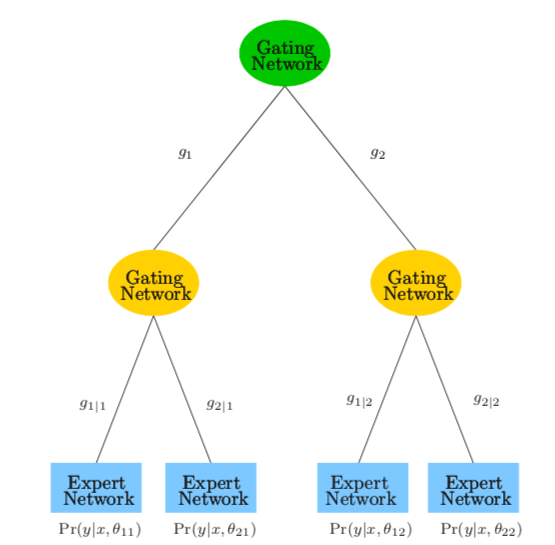
\includegraphics[scale=0.5]{img/HME}
\caption{A two-level HME model.}
\end{figure}
\subsubsection{How HME works}
Consider the data $(x_i, y_i), \quad i=1,\cdots, N$ either for regression or classification problem. The \textbf{top-gating} network has the output:
\begin{equation}
g_j(\x, \gamma_j) = \frac{e^{\gamma_j^T\x}}{\sum_{k=1}^Ke^{\gamma_k^T\x}}, \quad\quad j=1,\cdots, K
\end{equation}
where $\gamma_j$ is a vector of unknown parameters. Each $g_j$ is the probability of assigning an observation with feature vector $\x$ to the $j-th$ branch (soft $K$-way split). At second level the \textbf{gating networks} have similar form:
\begin{equation}
g_{\ell|j}(\x, \gamma_{j|\ell}) = \frac{e^{\gamma_{j|\ell}^T\x}}{\sum_{k=1}^Ke^{\gamma_{j|k}^T\x}}, \quad\quad \ell=1,
\end{equation}
This is the probability of assignment to the $l-th$ branch, given assignment to the $j-th$ branch at the level above. At each expert (terminal node), we have a model for the response variable of the form:
\begin{equation}
Y \sim Pr(y|\x, \theta_{j\ell}
\end{equation}
which is different according to the type of problem. For \textbf{regression} the Gaussian linear model is used with $\theta_{j\ell} = (\beta_{j\ell},\sigma^2_{jl}$:
\begin{equation}
Y = \beta_{j\ell}^Tx + epsilon, \quad\quad \CMcal{N} \sim(0,\sigma^2_{jl}). 
\end{equation}

For \textbf{classification} the linear logistic regression is used:
\begin{equation}
Pr(Y=1|\x, \theta_{j\ell} = \frac{1}{1+e^{-\theta_{j\ell}^T\x}}
\end{equation}
Denoting with $\Phi = \{\gamma_j,\gamma_{j\ell}, \theta_{j\ell}\}$ the collections of all parameters, the total probability that $Y=y$ is:
\begin{equation}
Pr(y|\x, \Phi) = \sum_{k=1}^K g_j(x, \gamma_j)\sum_{\ell=1}^K g_{\ell|j}(\x, \gamma_{j\ell})Pr(y|\x,\theta_{j\ell})
\end{equation}
To estimate the parameters we maximize the log-likelihood of the data over $\Phi$. The most convenient method is the EM algorithm.

\subsection{Missing data}
The usual approach is to fill-in missing values. Roughly speaking, data are missing at random if the mechanism resulting in its omission is independent of its (unobserved) value. A more precise definition is given in Little and Rubin (2002). Suppose $y$ is the response vector and $X$ is the $N \times p$ matrix of inputs (some of which are missing). Denote by $X_{obs}$ the observed entries in $X$ and let $\mathbf{Z} = (y, X)$, $\mathbf{Z}_{obs} = (\y, \X_{obs})$. Finally, if $\mathbf{R}$ is an indicator matrix with $ij-th$entry 1 if $x_{ij}$ is missing and zero otherwise, then the data is said to be missing at random (MAR) if the distribution of $\mathbf{R}$ depends on the data $\mathbf{Z}$ only through $Z_{obs}$:
\begin{equation}
Pr(\mathbf{R}|\mathbf{Z},\theta) = Pr (\mathbf{R}|\mathbf{Z}_{obs},\theta)
\end{equation}
Data are said to be \textbf{missing completely at random (MCAR)} if the distribution$\mathbf{R}$ does not depend on the observed or missing data:
\begin{equation}
Pr(\mathbf{R}|\mathbf{Z},\theta) = Pr (\mathbf{R}|\theta)
\end{equation}
For example, if a patient’s measurement was not taken because the doctor felt he was too sick, that observation would not be MAR or MCAR.

Assuming the features are missing completely at random, there are a number of ways of proceeding:

\begin{enumerate}
\item \label{Missingi}Discard observations with any missing values.
\item \label{Missingii}Rely on the learning algorithm to deal with missing values in its training phase.
\item \label{Missingiii}Impute all missing values before training.
\end{enumerate}

Approach \autoref{Missingi} can be used if the relative amount of missing data is small, but otherwise should be avoided. Regarding \autoref{Missingii}, CART is one learning algorithm that deals effectively with missing values, through surrogate splits. MARS and PRIM use similar approaches. In generalized additive modeling, all observations missing for a given input feature are omitted when the partial residuals are smoothed against that feature in the backfitting algorithm, and their fitted values are set to zero. Since the fitted curves have mean zero (when the model includes an intercept), this amounts to assigning the average fitted value to the missing observations.
For most learning methods, the imputation approach \autoref{Missingiii} is necessary. The simplest tactic is to impute the missing value with the mean or median of the non-missing values for that feature.

If the features have at least some moderate degree of dependence, one can do better by estimating a predictive model for each feature given the other features and then imputing each missing value by its prediction from the model, distinctly from the method used to predict $y$ from $\x$.

\section{Boosting and Additive Trees}
\subsection{Boosting methods}
 It was originally designed for classification problems but it can profitably be extended to regression as well. The motivation for boosting was a procedure that combines the outputs of many "weak" classifiers to produce a powerful "committee".

A weak classifier is one whose error rate is only slightly better than random guessing. The purpose of boosting is to sequentially apply the weak classification algorithm to repeatedly modified versions of the data, thereby producing a sequence of weak classifiers $G_(x), \quad m=1,\cdots, M$. 
Consider a two-class problem with the output variable coded as $Y\in\{-1,1\}$. Given a vector of predictors $\X$, a classifier $G(X)$ produces a prediction taking one of the two values $\{-1,1\}$.
The predictions from all of them are then combined to through a weighted majority of vote to produce the final prediction:
\begin{equation}
G(x) = sign\br{\sum_{i=1}^M \alpha_mG_m(x)}
\end{equation}
This is the \textbf{AdaBoost} procedure. Here $\alpha_1, \cdots, \alpha_m$ are computed by the boosting algorithm and weight the single contribution. The data modifications at each boosting step consist of applying weights $w_1, \cdots, w_N$ to each of the training observations. Initially all the weights are $1/N$. For successive iterations,  the observation weights are individually modified and the classification algorithm is reapplied to the weighted observations. At step $m$ the observations that were misclassified by the classifier $G_{m-1}(x)$ have their weights increased, whereas the weights are decreased for those that were classified correctly. Thus as iterations proceed, observations that are difficult to classify correctly receive ever-increasing influence. Each successive classifier is thereby forced to concentrate on those training observations that are missed by previous ones in the sequence.
 
 The \textbf{AdaBoost.M1} algorithm, aka \textbf{Discrete Adaboost}, is shown in \autoref{AdaBoost.M1}. If the base classifier instead returns a real-valued prediction (e.g., a probability mapped to the interval $[-1,1]$), AdaBoost can be modified appropriately and becomes \textbf{Real Adaboost}.
 \begin{algorithm}[!ht]
    $w_i=1/N, \quad i=1,\cdots,N$
    
	\For{($m =1:M$)}{
			Fit a classifier $G_m(x)$ to training data using $w_i$;\\
			Compute the training error \begin{equation}
			err_m = \frac{\sum_{i=1}^N w_i I(y_i\ne G_m(x_i))}{\sum_{i=1}^N w_i};
			\end{equation}\\
			Compute $\alpha_m = \log\frac{1-err_m}{err_m}$;\\
			$w_i\leftarrow w_i e^{\alpha_m I(y_i\ne G_m(x_i))}, \quad i=1,\cdots, N$;\\
		}
		return $G(x) = sign\br{\sum_{i=1}^M \alpha_mG_m(x)}$
\caption{AdaBoost.M1 algorithm.}
\label{AdaBoost.M1}
\end{algorithm}
The power of AdaBoost to dramatically increase the performance of even a very weak classifier.

\subsection{Boosting fits an additive model}
Boosting is a way of fitting an additive expansion in a set of basis-functions where the basis functions are the individual classifiers. The basis function expansion takes the form:
\begin{equation}
f(x) = \sum_{m=1}^M \beta_m b(x, \gamma_m)
\end{equation}
Typically these models are fit by minimizing a loss function averaged over the training data, such as the squared error or a likelihood-based loss function:

\begin{equation}
\min_{\{\beta_m, \gamma_m\}_1^M} \sum_{i=1}^N L\br{y_i, \sum_{m=1}^M \beta_m b(x_i, \gamma_m)}
\label{additivCostEq}
\end{equation}
This is sometimes computationally infeasible and it is approximated by:
\begin{equation}
\min_{\{\beta_m, \gamma_m\}_1^M} \sum_{i=1}^N L\br{y_i, \beta b(x_i, \gamma)}
\end{equation}
\subsection{Forward Stagewise Additive Modeling}
Forward stagewise modelling approximates the solution of \autoref{additivCostEq} by sequentially adding new basis functions to the expansion without adjusting the parameters and coefficients of those that have already been added. At each iteration $m$ one solves for the optimal basis function $b(x, \gamma_m)$ and corresponding coefficient $\beta_m$ to add the current expansion $f_{m-1}(x)$. This produces $f_m(x)$ and the process is repeated. For squared error loss one has:
\begin{equation}
\begin{aligned}
L(y_i, f_{m-1}(x_i)+\beta b(x_i, \gamma)) &= (y_i-f_{m-1}(x_i)-f_{m-1}(x_i)-\beta b(x_i, \gamma))^2 =\\
 &=(r_i-\beta b(x_i, \gamma))^2
\end{aligned}
\end{equation}
The term that best fits the residual is added to the expansion at each step.

Stagewise additive modelling is equivalent to AdaBoost.M1 using the exponential loss-function:
\begin{equation}
L(y, f(x))  = exp(-yf(x))
\end{equation}
The principal attraction of exponential loss in the context of additive modeling is computational; it leads to the simple modular reweighting AdaBoost algorithm.

\section{Procedure for datamining}
In data mining applications, usually only a small fraction of the large number of predictor variables that have been included in the analysis are actually relevant to prediction. Also, unlike many applications such as pat- tern recognition, there is seldom reliable domain knowledge to help create especially relevant features and/or filter out the irrelevant ones, the inclu- sion of which dramatically degrades the performance of many methods.
In addition, data mining applications generally require interpretable mod- els. It is not enough to simply produce predictions. It is also desirable to have information providing qualitative understanding of the relationship between joint values of the input variables and the resulting predicted re- sponse value. Thus, black box methods such as neural networks, which can be quite useful in purely predictive settings such as pattern recognition, are far less useful for data mining.

An "off-the-shelf" method is one that can be directly applied to the data without requiring a great deal of time- consuming data preprocessing or careful tuning of the learning procedure. Decision trees come closest to meeting the requirements for serving as an off-the-shelf procedure for data mining. They are relatively fast to construct and they produce interpretable models (if the trees are small). They naturally incorporate mixtures of numeric and categorical predictor variables and missing values. They are invariant under (strictly monotone) transformations of the individual predictors. As a result, scaling and/or more general transformations are not an issue, and they are immune to the effects of predictor outliers. They perform internal feature selection as an integral part of the procedure. They are thereby resistant, if not completely immune, to the inclusion of many irrelevant predictor variables. These properties of decision trees are largely the reason that they have emerged as the most popular learning method for data mining. Trees have one aspect that prevents them from being the ideal tool for predictive learning, namely inaccuracy. They seldom provide predictive accuracy comparable to the best that can be achieved with the data at hand.

\subsection{Boosting trees}
The boosted tree model is a sum of tress induced in a forward stagewise manner:
\begin{equation}
\begin{aligned}
f_M(x) &= \sum_{m=1}^M T(x, \Theta_m)\\
T(x, \Theta_m) &= \sum_{j=1}^J\gamma_j I(x \in R_j)
\end{aligned}
\end{equation}
where $\Theta_m$ is the vector of parameters. Considering a single tree, the parameters are found by minimizing the empirical risk:
\begin{equation}
\hat{\Theta} = \argmin{\Theta}{\sum_{j=1}^J\sum_{x_i \in R_j}L(y_i, \gamma_j)}
\end{equation}
Due to the combinatorial problem, we usually settle for suboptimal solutions, dividing the problem into two parts:
\begin{itemize}
\item \textbf{Finding $\gamma_j$ given $R_j$}: this is typically trivial and often $\hat{\gamma_j} = \bar{y}_j$, the mean of $y_i$ falling in region $R_j$.
\item \textbf{Finding $R_j$}: this is the difficult part. A typical strategy is to use a greedy top-down recursive partitioning  algorithm to find $R_j$.
\end{itemize}

The boosted tree is induced in a forward stagewise manner. At each step one must solve:
\begin{equation}
\hat{\Theta}_m = \argmin{\Theta_m}{\sum_{i=1}^N L\br{y_i, f_{m-1}(x_i)+T\br{x_i, \Theta_m}}}
\end{equation}
for the region set and constants $\Theta_m = \{R_{jm},\gamma_{jm}\}_1^{J_m}$ for the next tree, given the current model $f_{m-1}(x)$. Given $R_{jm}$, finding the optimal constants $\gamma_{jm}$ in each region is typically straightforward:
\begin{equation}
\hat{\gamma}_{jm} = \argmin{\gamma_{jm}}{\sum_{x_i \in R_{jm}}} L(y_i, f_{m-1}(x_i)+\gamma_{jm})
\end{equation}
Finding the regions is more difficult, and even more difficult than for a single tree.

Defining the loss function as
\begin{equation}
L(f) = \sum_{i=1}^N L(y_i, f(x_i))
\end{equation}
where $f$ is a sum of trees. So, $\hat{\mathbf{f}} =\argmin{\mathbf{f}}{L(\mathbf{f})}$, $\mathbf{f}=\{f(x_i1), f(x_2), \cdots, f(x_N)\}$. Numerical procedures exist to find $\hat{\mathbf{f}}$ as a sum of component vectors:
\begin{equation}
\mathbf{f}_M = \sum_{m=0}^M \mathbf{h}_m, \quad \mathbf{h}_m \in CMcal{R}^N
\end{equation}
with $\mathbf{f}_0=\mathbf{h}_0$ is an initial guess.

One optimization is the \textbf{Steepest descent}: $\mathbf{h}_m = -\rho_m \mathbf{g}_m$, $\mathbf{g}$ being the gradient of $L(f)$ evaluated at $\mathbf{f}_{m-1}$.

Another way is the \textbf{Gradient Boosting}. The gradient is trivial to calculate for any differentiable loss function but it is defined only at the training data points $x_i$ whereas the ultimate goal is to generalize it to new data not in the training set.

A possible resolution to this dilemma is to induce a tree $T(x, \Theta_m)$ at the m-th iteration whose predictions $t_m$  are as close as possible to the negative gradient. Using squared error loss to measure closeness:
\begin{equation}
\widetilde{\Theta}_m = \argmin{\Theta}{\sum_{i=1}^N \br{-g_{im}-T(x_i, \Theta)}^2}
\end{equation}
 \begin{algorithm}[!ht]
    $f_0\leftarrow \argmin{\gamma}{\sum_{i=1}^N L(y_i, \gamma)}$;\\
	\For{($m =1:M$)}{
		\For{($i =1:N$)}{
			$r_{im} = \left[ \frac{\partial L(y_i,f(x_i))}{\partial f(x_i)}\right]_{f-f_{m-1}}$;\\			
		}
		Fit a regression tree to the targets $r_{im}$ giving terminal regions $R_{jm}, \quad j=1,\quad, J_m$;\\
		\For{($i =1:J_m$)}{
			$\gamma_{jm} = \argmin{\gamma}{\sum_{x_j \in R_{jm}} L(y_i, f_{m-1}(x_i)+\gamma)}$;\\			
		}
		$f_m(x) \leftarrow f_{m-1}+\sum_{j=1}^{J_m} L(y_i, f_{m-1}(x_i)+\gamma)$;\\
		}
		return $\hat{f} = f_M(x)$
\caption{Gradient Tree Boosting algorirthm.}
\end{algorithm}
The algorithm for classification is similar. Two basic tuning parameters are the number of iterations $M$ and the sizes of each of the constituent trees $J_m, m=1,2,...,M$.

\subsection{Right-sized Trees for boosting}
[skipped, at least for now]

\subsection{Regularization}
Besides the size of the constituent trees, $J$, the other meta-parameter of gradient boosting is the number of boosting iterations $M$. Each iteration usually reduces the training risk $L(f_M )$, so that for $M$ large enough this risk can be made arbitrarily small. However, fitting the training data too well can lead to overfitting, which degrades the risk on future predictions. Thus, there is an optimal number $M*$ minimizing future risk that is application dependent. A convenient way to estimate $M*$ is to monitor prediction risk as a function of M on a validation sample. The value of M that minimizes this risk is taken to be an estimate of $M*$.
\subsubsection{Shrinkage}
Controlling the value of $M$ is not the only possible regularization strategy. Shrinkage techniques can be employed as well. The simplest implementation of shrinkage in this case is to scale the contribution of each tree by a factor $0<\nu<1$ when it is added to the current approximation:
\begin{equation}
f_m(X) = f_{m-1}(x) + \nu \sum_{i=1}^J \gamma_{jm}I(x \in R_{jm}).
\end{equation}
Smaller values of $\nu$ (more shrinkage) result in larger training risk for the same number of iterations $M$. Empirically it has been found (Friedman, 2001) that smaller values of $\nu$ favor better test error, and require correspondingly larger values of $M$. The best strategy appears to be to set $\nu$ to be very small ($\nu < 0.1$) and then choose $M$ by early stopping, however more iterations are needed so the computational cost is higher. 

%%%%%%%%%%%%%%%%%%%%%%%%%%%%%%%%%%%%%%%%%%%%%%%%%%%%%%%%%%
%%%%%%%%------------------------------NEW SECTION------------------------------%%%%%%%%%
%%%%%%%%%%%%%%%%%%%%%%%%%%%%%%%%%%%%%%%%%%%%%%%%%%%%%%%%%%
\newpage
\section{Support Vector Machines and Flexible Discriminants}
The optimal separating hyperplane separates the two classes and maximizes the distance to the closest point from either class (Vapnik, 1996). Not only does this provide a unique solution to the separating hyperplane problem, but by maximizing the margin between the two classes on the training data, this leads to better classification performance on test data.
\iffalse
Suppose $M$ is the distance. Then

\begin{equation}
\begin{aligned}
&\max\limits_{\beta,\beta_0, ||\beta||=1} M \\
& y_i(x_i^T\beta + \beta_0) \ge M
\end{aligned}
\end{equation}

We  can move the constrain on the module $\||\be||=1$ to the condition $\frac{1}{||\be||}y_i(x_i^T\beta + \beta_0) \ge M$, which redefines $\be_0$. 

For a pair of coefficients satisfying this inequalities, any positively scaled multiple satisfies them too, so we can set arbitrarily set $||\be||=\frac{1}{M}$:

\begin{equation}
\begin{aligned}
&\min_{\be, \be_0}{\frac{1}{2}||\be||^2}\\
\textit{subject to } &y_i(x_i^T\be+\be_0)\ge1
\end{aligned}
\end{equation}

With this constraint, a margin around the decision boundary with thick $\frac{1}{||\be||}$ is present. We choose $\be$ to maximize the thickness of margin margin.  This is a convex optimization problem. The Lagrange primal function to be minimized is:

\begin{equation}
\label{eq}
L_p = \frac{1}{2} ||\be||^2 = \sum_{i=1}^N \alpha_i\left[ y_i \br{x_i^T\be+\be_0}\right]

\end{equation}

and setting the derivatives to $0$:

\begin{equation}
\begin{aligned}
\be &= \sum_{i=1}^N \alpha_i y_i x_i
0  &= \sum_{i=1}^N \alpha_i y_i
\end{aligned}
\end{equation}

and substituting in \autoref{eq}:

\begin{equation}
\begin{aligned}
L_D = \sum_{i=1}^N \alpha_i -\frac{1}{2}\sum_{i=1}^N\sum_{k=1}^N \alpha_i \alpha_ky_iy_kx_i^Tx_k\\
\textit{subject to } \alpha_i\ge0 \textit{ and } \sum_{i=1}^N \alpha_iy_i=0
\end{aligned}
\end{equation}
\fi


The optimal hyperplane (or hard margin SVM) focuses more on points that counts, i.e., close to the border, that are called \tb{support vector}. For this reason it is more robust. LDA depends on all the data, even points faraway. If classes are really Gaussian LDA is optimal and separating hyperplane will pay a price for focusing on noisier data.
For logistic regression, if a separate hyperplane exists, since the log-likelihood can be driven to $0$.

When data are not separable there will be no feasible solution and an alternative formulation is needed. In this case the we allow some points to be beyond the margin and the problem is generally referred to as \ti{soft margin classification}.

First we analyze the hard margin SVM classification problem with the following steps, then extend it to the non perfectly separable case with the soft margin classification and finally show how it can work for regression as well.

\subsection{Hard margin Support Vector Machine classification}
\label{HardMarginSVM}
\textit{https://nlp.stanford.edu/IR-book/html/htmledition/support-vector-machines-the-linearly-separable-case-1.html}
\textit{https://www.youtube.com/watch?v=\_PwhiWxHK8o}

We will follow the following steps:

\begin{figure}
\centering
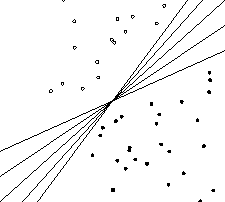
\includegraphics[scale=0.6]{img/separableClasses}
\caption{Example of infinite lines separating two perfectly separable classes.}
\label{separableClasses}
\end{figure}

Consider two classes on a space (for example a two dimensional space as in \autoref{separableClasses}) and suppose the two classes are perfectly separable. We want to divide the two classes with a straight line. The problem becomes to define what is the best straight line since such lines exist. The solution is to choose the line that separates the classes as much as possible, lying as faraway as possible from both the classes. Such line can be thought as the middle line of a street separating the two classes; then we want to fit the widest possible street between the two classes (see \autoref{separableClassesPy}). The closest occurrences of the two classes closest to the separator defines the margins, the gutters of the street (the dashed lines in \autoref{separableClassesPy}).

\begin{figure}
\centering
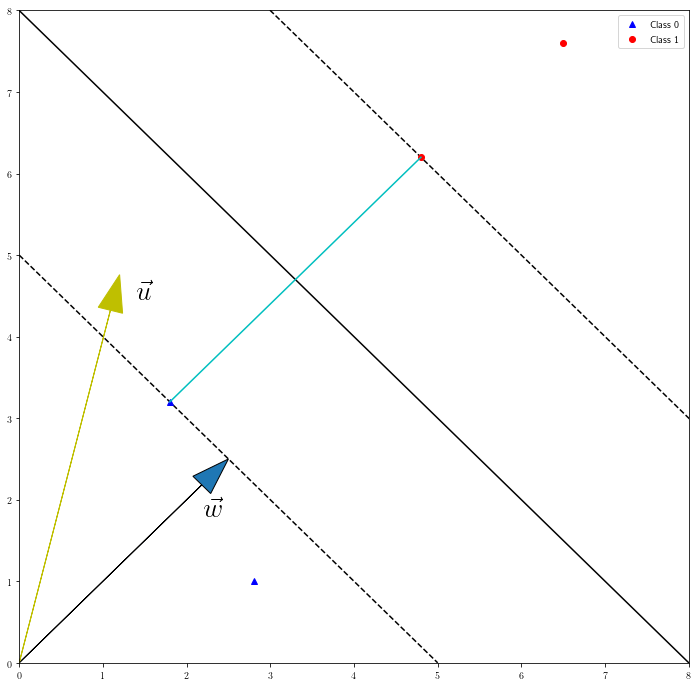
\includegraphics[scale=0.4]{img/separableClassesPy}
\caption{Example of best separating line maximizing the margin.}
\label{separableClassesPy}
\end{figure}

Let us consider a vector $\vec{w}$ of any length, perpendicular to the gutters of the street and consider an unknown instance to be classified (\autoref{separableClassesPy}) called $\vec{u}$. To see if this unknown is on the left or right side of the street, we project its vector $\vec{u}$ onto the vector $\vec{w}$ that is perpendicular to the street. The bigger this product, the more likely the point is to be on the right side of street, hence the more likely it is to be of class $+$.

Mathematically:
\begin{equation}
\vec{u}\cdot \vec{w} \ge c \Leftrightarrow \vec{u}\cdot \vec{w} + b \ge0\Rightarrow \text{Class } 1 \quad\quad \text{with } b=-c
\end{equation}
This is the \tb{decision rule}. The problem is that both $\vec{w}$ and $b$ are unknown; only the direction of $\vec{w}$ is known but not its length.

\tb{Other constraints must be added} to calculate $\vec{w}$ and $b$. Now suppose one positive and one negative instances $x_+$ and $x_-$ are given. We want:
\begin{equation}
\begin{aligned}
\vec{w} \cdot \vec{x}_+ + b &\ge 1\\
\vec{w} \cdot \vec{x}_- + b &\le -1
\end{aligned}
\end{equation}
Just for mathematical convenience we introduce a new variable $y_i$ for each instance such that:
\begin{equation}
\begin{aligned}
y_i = 1 \quad \text{if } \vec{x}_+\\
y_i = -1 \quad \text{if } \vec{x}_-\\ 
\end{aligned}
\end{equation}
In this way:
\begin{equation}
y_i (\vec{w}\cdot \vec{x}_i + b) \ge 1
\end{equation}
that can be rearranged as:
\begin{equation}
y_i (\vec{w}\cdot \vec{x}_i + b) -1 \ge 0
\end{equation}

Now \tb{another constraint} is going to be added: \tb{the previous equation is forced to be $0$ for the points in the gutter}, i.e., on the margins:
\begin{equation}
y_i (\vec{w}\cdot \vec{x}_i + b) -1 = 0
\label{SVMmargin}
\end{equation}

\begin{figure}
\centering
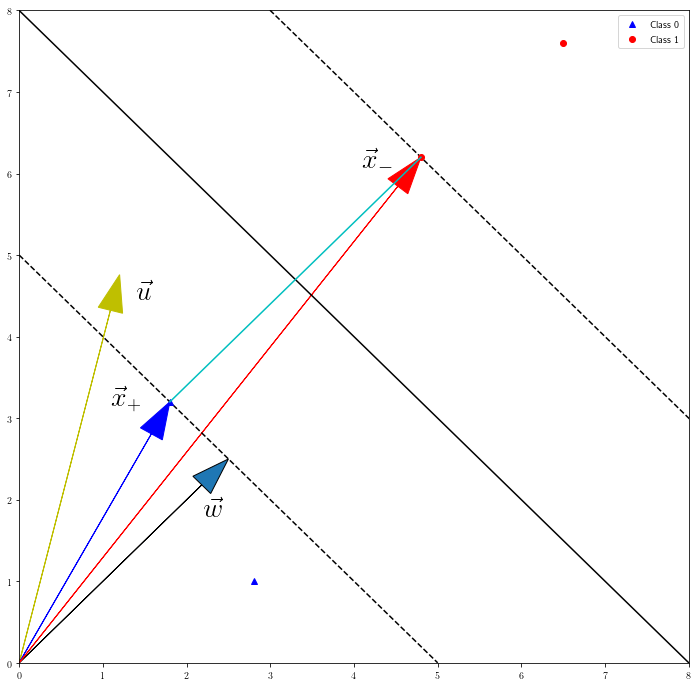
\includegraphics[scale=0.4]{img/SVMwidth}
\caption{Derivation of the width.}
\label{SVMwidth}
\end{figure}

So this equation holds for the points $x_+$ and $x_-$ that are closest to the separator (the black solid line on the previous plots), i.e., the ones that decide and limit the width of the street. Now we need to express the width of the street. Consider the difference between these two points $(\vec{x}_+ - \vec{x}_-)$ (\autoref{SVMwidth}) and project it onto the normal: \textbf{this is exactly the width of the street}.
\begin{equation}
\begin{aligned}
\text{width} = 2M = \left( \vec{x}_+ - \vec{x}_-\right) \cdot \frac{\vec{w}}{\norm{\vec{w}}}
\end{aligned}
\label{width0}
\end{equation}

For $\vec{x}_+$, $y_i=1$. From \autoref{SVMmargin}:
\begin{equation}
\vec{w} \vec{x}_+ + b = 1\Rightarrow \vec{w} \vec{x}_+ = 1-b
\end{equation}
for the same reason, considering $x_-$:
\begin{equation}
-\vec{w} \vec{x}_- - b = 1\Rightarrow -\vec{w} \vec{x}_+ = 1+b
\end{equation}

So substituting in \autoref{width0}:
\begin{equation}
\begin{aligned}
\text{width} = \frac{2}{\norm{\vec{w}}}
\end{aligned}
\label{width1}
\end{equation}

\tb{Now we have to maximize the width}:
\begin{equation}
\max \frac{2}{\norm{\vec{w}}} \Leftrightarrow \max \frac{1}{\norm{\vec{w}}} \Leftrightarrow\min \norm{\vec{w}} \Leftrightarrow \min \frac{1}{2} \norm{\vec{w}}^2
\label{SVMmin}
\end{equation}

We have the expression \autoref{SVMmin} for which we want to find the minimum, its extreme, and we have the constraint \autoref{SVMmargin}. By \tb{Lagrange}, if we want to find the extreme of a function with constraints, then we have to use \tb{Lagrange multipliers} which will result in a new expression that can be maximized or minimized directly without any constraint. 
\begin{equation}
L(\vec{w}, b) = \frac{1}{2}\norm{\vec{w}}^2 - \sum_i \alpha_i\left[ y_i\left( \vec{w}\cdot \vec{x}_i+b\right)-1\right]
\label{SVMLagranceMult}
\end{equation}
where the second term is a sum of all the constraints weighted by $\alpha_i$, the Lagrange multipliers. These multipliers will be different from $0$ for only the points in the gutter; if the same class has more than one point on the margin then all of them will be part of the expression. We need to find the extreme of this expression. To do that, we take the derivatives and set them to $0$.
\begin{equation}
\begin{aligned}
&\frac{\partial L}{\partial \vec{w}} = w - \sum_i \alpha_i y_i \vec{x}_i = 0 \Rightarrow &\vec{w} = \sum_i \alpha_i y_i \vec{x}_i
\end{aligned}
\label{SVMLagrDevw}
\end{equation}
This tells that the vector $\vec{w}$ is a linear combination of all the sample vectors lying on the margin, the \tb{support vector}.

Differentiating with respect to $b$:
\begin{equation}
\begin{aligned}
&\frac{\partial L}{\partial b} = \sum_i \alpha_i y_i = 0 \Rightarrow \sum_i \alpha_i y_i = 0
\end{aligned}
\label{SVMLagrDevb}
\end{equation}

We try to substitute these results in \autoref{SVMLagranceMult} to find its extreme:
\begin{equation}
\begin{aligned}
L &= \frac{1}{2} \left(  \sum_i \alpha_i y_i \vec{x}_i\right) \left( \sum_j \alpha_j y_j \vec{x}_j\right) - \sum_i \alpha_i y_i \vec{x}_i \cdot\left(\sum_j \alpha_j y_j \vec{x}_j\right) -\sum_i \alpha_i y_i b + \sum_i \alpha_i =\\
& = \frac{1}{2} \left(  \sum_i \alpha_i y_i \vec{x}_i\right) \left( \sum_j \alpha_j y_j \vec{x}_j\right) - \sum_i \alpha_i y_i \vec{x}_i \cdot\left(\sum_j \alpha_j y_j \vec{x}_j\right) -b \cancel{\sum_i \alpha_i y_i} + \sum_i \alpha_i  =\\
&= \sum_i \alpha_i - \frac{1}{2}\sum_i \sum_j \alpha_i \alpha_j y_i y_j \vec{x}_i \cdot \vec{x}_j 
\end{aligned}
\end{equation}
where $b$ has been taken out of the sum since it is a constant. This expression allows to see what the value of the extreme point depends on with respect to these vectors. It depends only on the dot product of pairs of samples.

Let us see how the decision rule is affected:
\begin{equation}
\sum_i \alpha_i y_i \vec{x}_i \cdot \vec{u} + b \ge 0 \Rightarrow \vec{u} \text{ belongs to class } +
\end{equation}

Note that the space we are working on is a convex space, so there is no chance to get stuck in a local minimum/maximum, as opposite to neural nets.

This process does not work with linear inseparable problems. In these cases we can switch to another space: we call this transformation $\phi(\vec{x})$. The maximization process depends only on the dot product, so we just need to find $\phi(\vec{x}_i)\cdot \phi(\vec{x}_j)$ in order to maximize in the new space. So actually the mapping function $\phi(\cdot)$ is not needed to be known, we need to know a function such as
\begin{equation}
K(\vec{x}_i, \vec{x}_j) = \phi(\vec{x}_i)\cdot \phi(\vec{x}_j)
\end{equation} 
Such a function is called \tb{Kernel function}. Popular choices of kernels are
\begin{itemize}
\item linear kernel $\left(\vec{u} \cdot \vec{v}+1\right)^n$
\item $e^{-\frac{\norm{\vec{x}_i - \vec{x}_j}}{\sigma}}$: be careful to choose a not too small $\sigma$ the points are shrunk around and we get overfitting.
\end{itemize}

We have seen \textbf{Optimal separating hyperplabes} in \autoref{OSH}. Here we will see the case for non-separable classes, where the classes overlap.
\subsection{Soft Margin Support Vector Machine}
The hard margin SVM works well when data do not contain outliers or noisy samples close to the separator. In such cases, the outlier can make the margin too small or move the separator toward the other class and this might cause misclassification. It is generally preferable to have a fat margin allowing to some noisy samples to be inside or on the wrong side of the margin.

We still want to maximize the margins $M$ allowing some points to be on the wrong side. For each misclassified point we pay a cost proportional to its distance from the margin. To do this, we define a slack variable $\xi=\br{\xi_1, \xi_2, \cdots, \xi_N}$ with $\xi_i\ge 0$, whose value is not null for the points beyond the margin:
\begin{equation}
\xi_i = \max \left(0, 1-y_i(\vec{w}\vec{x_i}+b)\right)
\end{equation}
where $1-y_i(\vec{w}\vec{x_i}+b)$ is proportional to the distance from the margin.	
The decision rule hence becomes:
\begin{equation}
\begin{aligned}
& y_i \left( \vec{w} \vec{x}_i + b\right) \ge 1 - \xi_i \Rightarrow y_i \left( \vec{w} \vec{x}_i + b\right) - 1+ \xi_i  \ge 0 \\
& \xi_i \ge 0
\end{aligned}
\end{equation}
However, we want to limit the number of misclassified points so the objective becomes
\begin{equation}
\begin{aligned}
&\min \frac{1}{2} \norm{\vec{w}} + C \sum_i \xi_i\\
\textit{subject to }&\left\{
		\begin{array}{ll}
				y_i(\vec{w} \cdot \vec{x}_i+b) \ge 1-\xi_i\\ 
 				\xi_i \ge 0
		\end{array} 
\right.
\end{aligned}
\end{equation}
The width remains the same as the one in \autoref{HardMarginSVM}. 

\iffalse
\subsubsection{}
With $N$ pairs $(x_i, y_i) \in \CMcal{R}^p$ and $y_i \in \{-1, 1\}$, define a hyperplane:
\begin{equation}
\{x: f(x) = x^T\beta+ \beta_0=0\}
\end{equation}
where $\left|\beta\right|=1$ is a unit vector. A classification rule induced by $f(x)$ is:
\begin{equation}
G(x) = sign\left[x^T\beta+\beta_0\right]
\end{equation}
When the classes are separable, we can find a function $f(x)=x^T\beta+\beta_0$ with $y_if(x_i)>0, \quad \forall i$. Hence, we are able to find the hyperplane creating the biggest margin between training points belonging to the two different classes:
\begin{equation}
\begin{aligned}
&\max_{\beta, \beta_0,\left|\beta\right|=1} M\\
&\textit{subject to } y_i(x_i^T\beta+\beta_0)\ge M,\quad i=1,\cdots,N
\end{aligned}
\end{equation}
or equivalently:
\begin{equation}
\begin{aligned}
&\min_{\beta, \beta_0} \left|\beta\right|\\
\textit{subject to } \quad&y_i(x_i^T\beta+\beta_0)\ge 1,\quad i=1,\cdots,N
\end{aligned}
\end{equation}
$M$ is the distance from the hyperplane to the wider side and it is called \textbf{margin}. This is a convex optimization problem.


\textbf{Suppose that the classes overlap in the feature space}. We still want to maximize $M$ allowing some points to be on the wrong side. We define a slack variable $\xi=\br{\xi_1, \xi_2, \cdots, \xi_N}$. There are two ways to modify the constraint:
\begin{equation}
\begin{aligned}
&y_i (x_i^T\beta+\beta_0)\ge M -\xi_i\\
\textit{or} \quad&y_i (x_i^T\beta+\beta_0)\ge M (1-\xi_i)\\
&\forall i, \xi_i\ge  0, \sum_{i=1}^N \xi_i \le constant.
\end{aligned}
\end{equation}
The two choices lead to different solutions. The first choice is more natural since it measures overlap in actual distance from the margin. The second choice measures the overlap in relative distance, which changes the width of the margin $M$. However, the first choice leads to a nonconvex optimization, while the second results to the standard support vector classifier.


The value $\xi_i$ is the proportional amount by which the prediction $f(x_i) = x_i^T\beta+\beta_0$ is on the wrong side of the margin. Hence by up-bounding the sum $\sum \xi_i$ we limit the total proportional amount by which predictions fall on the wrong side. Misclassifications occur when $\xi_i> 1$. So using  a constant $K$ one bounds the total number of misclassifications to $K$. Again, we can drop the norm constraint on $\beta$:
\begin{equation}
\begin{aligned}
&M = \frac{1}{\left| \beta\right|}\\
\textit{subject to } &\left\{
		\begin{array}{ll}
				y_i(x_i^T\beta +\be_0) \ge 1-\xi_i \quad \forall i \\ 
 				\xi_i \ge 0\\
 				\sum_i \xi_i \le constant
		\end{array} 
\right.
\end{aligned}
\label{SVMOpt}
\end{equation}
\begin{figure}
\centering
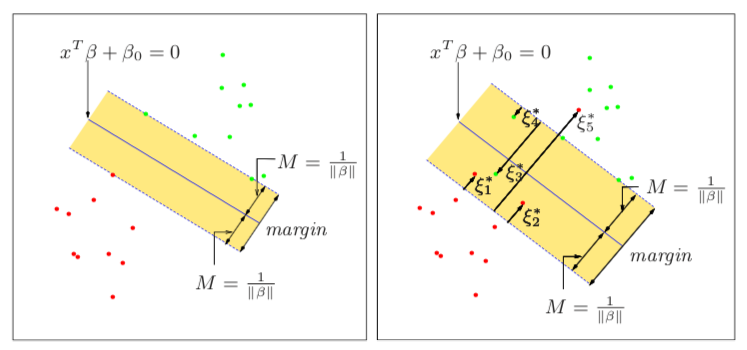
\includegraphics[scale=0.5]{img/SVM}
\caption{Separable and non separable support vector classifiers.}
\end{figure}
The misclassified points are on the wrong side for an amount $\xi^* = M \xi$ while the correctly classified points have $\xi^*=0$. One sees that points inside their class boundary do not play a big role in shaping the boundary. This seems like an attractive property, and one that differentiates it from linear discriminant analysis (\autoref{LDA}). In LDA, the decision boundary is determined by the covariance of the class distributions and the positions of the class centroids. Logistic regression is more similar to the support vector classifier in this regard.

\subsubsection{Computing the support vector classifier}

The problem \autoref{SVMOpt} is quadratic with linear inequality constraints, hence it is a convex optimization problem. We describe a quadratic programming solution using Lagrange multipliers. Computationally it is convenient to re-express \autoref{SVMOpt} in the equivalent form:
\begin{equation}
\begin{aligned}
&\min_{\beta, \beta_0} \frac{1}{2}\left|\beta\right|^2 + C\sum_{i=1}^N \xi_i\\
\textit{subject to } &\xi \ge 0, \quad y_i(x_i^T\beta+\beta_0)\ge 1-\xi_i \quad\forall i
\end{aligned}
\end{equation}
where $C$ replaces the constant. The separable case corresponds to $C = \infty$.
\subsubsection{}
\fi

The problem is quadratic with linear inequalities, hence it is still convex. The Lagrange primal function becomes:
\begin{equation}
L_P = \frac{1}{2}\norm{ \vec{w}}^2 + C \sum_{i=1}^N \xi_i - \sum_{i=1}^N \alpha_i \left[y_i\br{
\vec{w} \cdot \vec{x}_i+b}-\br{1-\xi_i}\right] - \sum_{i=1}^N \mu_i \xi_i 
\label{Lp}
\end{equation}
where $\mu_i$ are the Lagrange multipliers for the newly introduced constraint $\xi_i\ge 0$.
We minimize w.r.t. $\vec{w}, b, \xi_i$. The first two have already been calculated in \autoref{SVMLagrDevw} and \autoref{SVMLagrDevb}:
\begin{equation}
\begin{aligned}
\frac{\partial L_P}{\partial \xi_i} = \Rightarrow \alpha_i &= C - \mu_i \quad \forall i\\
\end{aligned}
\end{equation}
Substituting in \autoref{Lp}, we obtain the Lagrangian (Wolfe) dual objective function:
\begin{equation}
\begin{aligned}
L_D &=  \frac{1}{2}\norm{ \vec{w}}^2 + \cancel{C \sum_{i=1}^N \xi_i} - \sum_{i=1}^N \alpha_i \left[y_i\br{
\vec{w} \cdot \vec{x}_i+b} -1\right]+\cancel{\alpha_i\br{\xi_i}} - \cancel{\sum_{i=1}^N \mu_i \xi_i} = \\
&=\frac{1}{2}\sum_{i=1}^N  \alpha_i y_i \vec{x}_i \cdot \sum_{j=1}^N  \alpha_j y_j \vec{x}_j- \sum_{i=1}^N \alpha_i y_i \vec{x}_i\vec{w} \cancel{- b\sum_{i=1}^N \alpha_i y_i}+ \sum_{i=1}^N \alpha_i =\\
&=\frac{1}{2}\sum_{i=1}^N  \alpha_i y_i \vec{x}_i \cdot \sum_{j=1}^N  \alpha_j y_j \vec{x}_j- \sum_{i=1}^N \alpha_i y_i \vec{x}_i\sum_{j=1}^N \alpha_j y_j \vec{x}_j+ \sum_{i=1}^N \alpha_i =\\
&= \sum_{i=1}^N \alpha_i - \frac{1}{2}\sum_{i=1}^N \alpha_i y_i \vec{x}_i\sum_{j=1}^N \alpha_j y_j \vec{x}_j = \sum_{i=1}^N \alpha_i - \frac{1}{2}\sum_{i=1}^N\sum_{j=1}^N \alpha_i y_i \alpha_j y_j\vec{x}_i  \vec{x}_j
\end{aligned}
\label{LagrangeDueal}
\end{equation}
where we used the properties that $\alpha_i, y_i$ are scalar and that $\vec{w}, b$ can be taken out. Notice that $\vec{w}\cdot \vec{w}  = \sum_{i=1}^N \alpha_i y_i \vec{x}_i\cdot\sum_{j=1}^N\alpha_j y_j \vec{x}_j =\sum_{i=1}^N \sum_{j=1}^N \alpha_i y_i \alpha_j y_j  \vec{x}_i\vec{x}_j \ne \sum_{i=1}^N  (\alpha_i y_i)^2 \vec{x}_i\vec{x}_i$. In fact consider for example: $\vec{w} = c_1\vec{x}_1 + c_2\vec{x}_2$ with $\vec{x}_i = \left[x_{1i}, x_{2i}\right]^T$. $\vec{w} = \left[ c_1x_{11}+c_2x_{12}, c_1x_{21}+c_2x_{22} \right]^T$ and $\vec{w}\cdot \vec{w} = (c_1x_{11}+c_2x_{12})^2+(c_1x_{21}+c_2x_{22})^2$, so we are missing some cross-products. The Lagrangian (Wolfe) dual objective function gives a lower bound on the objective function for any feasible point. We maximize $L_D$ subject to $0\le \alpha_i\le C$ and $\sum_{i=1}^N\alpha_iy_i$. In addition to the derivatives, the \textbf{Karush-kuhn-Tucker} conditions include constraints:
\begin{equation}
\begin{aligned}
\alpha_i \left[ y_i\br{\vec{w}\cdot\vec{x}_i+b}-\br{1-\xi_i}\right] &=0\\
\mu_i \xi_i &= 0\\
y_i(\vec{x}_i\vec{w}+b) - (1 - \xi_i) &\ge 0
\end{aligned}
\label{KKT}
\end{equation}
for $i=1,\cdots, N$. These constraints and the ones originating from the derivatives uniquely characterize the primal and dual problem.

From $\vec{w} = \sum_{i=1}^N  \alpha_i y_i \vec{x}_i$, we can see:
\begin{equation}
\hat{\vec{w}} = \sum_{i=1}^N \hat{\alpha}_i y_i \vec{x}
\end{equation}
with $\hat{\alpha}_i \ne 0$ only for those observations $i$ for which the constraints in the last equation of \autoref{KKT} are exactly met. These observations are called \textbf{support vectors}, since $\hat{\vec{w}}$ is represented in terms of them alone. Among these support points, some will lie on the edge of the margin ($\hat{\xi}_i=0$) and hence will be characterized by $0 < \hat{\alpha_i} <C$: the remainder ($\hat{\xi}_i>0$) have $\hat{\alpha}_i=C$. We can see that any of these margin points ($0<\hat{\alpha}_i$, $\hat{\xi}_i = 0$), can be used to solve for $b$, and we typically use an average of all the solutions for numerical stability. Maximizing the dual is a simpler convex quadratic programming problem than the primal and can be solved with standard techniques such (Murray et. al, 1981).

Points on the wrong side of the boundary are support vectors. In addition, points on the correct side of the boundary but close to it (in the margin), are also support vectors. 

Given the solutions $\hat{\vec{w}}, \hat{b}$, the decision function can be written as:
\begin{equation}
\hat{G} (x) = sign \br{\hat{f}(x)}= sign\br{\hat{\vec{w}}\cdot \vec{x}_i+b}
\end{equation}
The tuning parameter of this procedure is the cost parameter $C$. The optimal value for C can be estimated by cross-validation.
\subsection{Support vector machines and Kernels}
We can make the procedure more flexible by enlarging the feature space using basis expansions such as polynomials or splines. Generally linear boundaries in the enlarged space achieve better training-class separation, and translate to nonlinear boundaries in the original space. 

\subsubsection{Computing SVM for classification}
The Lagrange dual function has the form:
\begin{equation}
L_D = \sum_{i=1}^N \alpha_i - \frac{1}{2}\sum_{i=1}^N\sum_{j=1}^N \alpha_i y_i \alpha_j y_j\left\langle  h(x_i), h(x_j)  \right\rangle 
\end{equation}
So $f(x)$ can be written as 
\begin{equation}
f(x) = h(x)\cdot\vec{w} + b = \sum_{i=1}^N \alpha_iy_i \left\langle  h(x), h(x_i)  \right\rangle +b
\end{equation}

As before, given $\alpha_i$, $b$ can be determined by solving $y_i f(x_i) = 1$ for any (or all) $x_i$ for which $0<\alpha_i <C$.
So $h(x0)$ is involved only in terms of its inner product: \textbf{we do not need to specify the transformation but only the knowledge of the kernel function is required}:
\begin{equation}
K(x, x') = \left\langle  h(x), h(x')  \right\rangle
\end{equation}
$K$ should be symmetric positive (semi-) definite.   Possible popular choices are:

\begin{equation}
\begin{aligned}
\textbf{dth-Degree polynomial:} &\quad K(x, x') = \br{1+\left\langle  x,x'  \right\rangle}^d\\
\textbf{Radial basis:} &\quad K(x, x') =e^{-\gamma\left| x-x' \right|^2}\\
\textbf{Neural Network:} &\quad K(x, x') = tanh\br{k_1\left\langle  x,x'  \right\rangle+k_2}\\
\end{aligned}
\end{equation}
\subsection{SVM for Regression}
SVM can be adapted for regression. The linear regression model is in the form
\begin{equation}
f(x) = x^T\be+\be_0
\end{equation}
and then handle non-linear generalizations. To estimate $\be$ we consider minimization of:
\begin{equation}
\begin{aligned}
H(\be, \be_0) &= \sum_{i=1}^NV\br{y_i - f(x_i)}+\frac{\lambda}{2}\left|\be\right|^2\\
V_\epsilon &=\left\{\begin{array}{ll}0 \quad \quad \textit{if}\quad |r|<1 \\ 
 |r|-\epsilon  \quad \quad \textit{otherwise}
\end{array} 
\right.
\end{aligned}
\end{equation}
\begin{figure}
\centering
\includegraphics[scale=0.5]{img/RegSVMV}
\caption{The left panel shows the $\epsilon$-insensitive error function used by the support vector regression machine. The right panel shows the error function used in Huber’s robust regression (blue curve) used in statistics. Beyond $|c|$, the function changes from quadratic to linear reducing the contribution of outliers.}
\label{RegSVMV}
\end{figure}
This is an "$\epsilon$-insensitive" error measure, ignoring errors of size less than $\epsilon$ (left panel of \autoref{RegSVMV}). There is a rough analogy with the support vector classification setup, where points on the correct side of the decision boundary and far away from it, are ignored in the optimization. In regression, these "low error" points are the ones with small residuals.

The support vector error measure has linear tails (beyond $\epsilon$), but in addition it flattens the contributions of those cases with small residuals.

If $\be, \be_0$ are the minimizers of $H$, the solution function can be shown to have the form:
\begin{equation}
\begin{aligned}
\hat{\be} &= \sum_{i=1}^N(\hat{\alpha}_i^* - \hat{\alpha}_i)x_i\\
\hat{f}(x) &= \sum_{i=1}^N(\hat{\alpha}_i^* - \hat{\alpha}_i)\left\langle x,x_i\right\rangle+\be_0
\end{aligned}
\end{equation}
where $\hat{\alpha}_i^*, \hat{\alpha}_i$ are positive and solve the quadratic problem:
\begin{equation}
\begin{aligned}
&min_{\alpha_i, \alpha_i^*}\epsilon \sum_{i=1}^N(\alpha_i^* + \alpha_i)-\sum_{i=1}^Ny_i(\alpha_i^* - \alpha_i)+\frac{1}{2}\sum_{i,j=1}^N(\alpha_i^* - \alpha_i)(\alpha_j^* - \alpha_j)\left\langle x_i,x_j\right\rangle\\
&\textit{subject to} \left\{ \begin{array}{lll}
		0 \le \alpha_i, \alpha_i^* \le \frac{1}{\lambda}\\
		\sum_{i=1}^N  (\alpha_i^* - \alpha_i) =0\\
		\alpha_i, \alpha_i^* = 0
		\end{array}
		\right.
\end{aligned}
\end{equation}
Due to the nature of these constraints, typically only a subset of the solution values $(\hat{\alpha}_i^* - \hat{\alpha}_i^*)$ are nonzero, and the associated data values are called the support vectors.
There are two parameters: $\epsilon$ is a parameter of the loss function. $\lambda$ is a regularization parameter and can be estimated by cross validation.

\textbf{The SVM can be extended to multiclass problems} by solving many two-class problems. A classifier is built for each pair of classes and the final classifier is the one that dominates the most.

\subsection{Generalized  LDA}
LDA is a simple prototype classifier which classifies points closest to the centroid. LDA is the estimated Bayes classifier if the observations are multivariate Gaussian in each class, with common covariance matrix, which is very unlikely. LDA has linear boundaries and provides natural low-dimensional views of data. Despite these properties, it fails in a number of situations. One is when more flexibility at for the boundaries is required; in this case QDA works. It does not work well neither with too many correlated predictors, for example in case of digitalized analogue signals and images, since in this case it uses too many parameters. Finally, LDA assumes a single centroid (prototype) per class (and a common covariance matrix) to describe the spread of the data in each class. Sometimes  several centroids are more appropriate.

Three alternatives exist to these three situations:
\begin{itemize}
\item \textbf{recast the LDA problem as a linear regression problem}, which in turn can be converted to a non-parametric form of regression, achieving more flexibility. These are called \textbf{FDA}. The regression procedures can be seen to identify an enlarged set of predictors via basis expansions. FDA amounts to LDA in this enlarged space.
\item When there are too many predictors, we do not want to expand the set. The second idea is to fit LDA but penalize its coefficients to be smooth or otherwise coherent in the spatial domain, such as an image. This is called \textbf{Penalized Discriminant Analysis (PDA)}.
\item \textbf{Model each class by a mixture of two or more Gaussians with different centroids sharing the same covariance matrix}. This allows for more complex decision boundaries and allows for subspace reduction. This is called \textbf{Mixture Discriminant Analysis (MDA)}.
\end{itemize}

\subsubsection{Flexible Discriminant Analysis (FDA)}
This technique performs LDA using linear-regression on derived responses.
Assume we have observations with a quantitative response $G$ falling into one of $K$ classes. Suppose $\theta:\CMcal{G} \rightarrow \CMcal{R}^1$ is a function that assigns scores to the classes such that the transformed class labels are optimally predicted by linear regression, producing the derived responses. Then, having as training examples $(g_i, x_i)$, we solve:
\begin{equation}
\min_{\theta, \be} \sum_{i=1}^N \br{\theta(g_i)-x_i^T\be}^2
\end{equation}
with restrictions on $\theta$ to avoid trivial solutions(mean zero and unit variance over the training data).

More generally, we can find up to $L \le K-1 $ sets of independent scorings for the class labels, $\theta_1, \theta_2, \cdots , \theta_L$, and $L$ corresponding linear maps $\eta_\ell(X) = X^T \be_\ell, l = 1,\cdots, L$, chosen to be optimal for multiple regression in $\CMcal{R}^p$. So the mapping function for one class does not to be the same for the others.

The scores $\theta_\ell(g)$ and maps $\be_\ell$ are chosen to minimize the average squared residual:
\begin{equation}
ASR = \frac{1}{N}\sum_{\ell=1}^N\left[ \br{\theta_\ell(g_i) - x_i^T\be_k}^2\right]
\end{equation}
The set of scores are assumed to be mutually orthogonal and normalized with respect to an appropriate inner product to prevent trivial zero solutions.

The Mahalanobis distance of a test point $x$ to the $k-th$ class centroid $\hat{\mu}_k$ is given by:
\begin{equation}
\delta_j (x, \hat{\mu}_k) = \sum_{\ell=1}^{K-1} w_\ell \br{\hat{\eta}_\ell(x) - \eta_\ell^{-k}(x) }+D(x)
\end{equation}
where $\eta_\ell^{-k}(x) $s is the mean of $\hat{\eta}_\ell(x)$ in the $k-th$ class, and $D(x)$ does not depend on $k$ and $w_\ell$ are defined in terms of the mean squared residual $r_\ell^2$ f the $\ell$th optimally scored fit:
\begin{equation}
w_\ell = \frac{1}{r_\ell^2(1-r_\ell^2}
\end{equation}
To summarize, LDA can be performed by a sequence of linear regressions, fol- lowed by classification to the closest class centroid in the space of fits.

The power is that we can replace the linear regression with more flexible non-parametric fits, achieving a more flexible classifier. We can use generalized additive fits, spline functions, MARS and others. In this more general form the regression problems are defined by the criterion:
\begin{equation}
ASR \br{\{\theta_\ell, \eta_\ell \}_{\ell=1}^L} = \frac{1}{N}\sum_{\ell=1}^L\left[\sum_{i=1}^N \br{\theta_\ell(g_i) - \eta_\ell(x_i)}^2 + \lambda J(\eta_\ell)\right]
\end{equation}
where $J$ is a regularizer appropriate for some forms of nonparametric regression.

The computations of FDA coordinates can be simplified in cases when the nonparametric procedure can be represented as a linear operator $\mathbf{S}_\lambda$, that is $\hat{\y} =\mathbf{S}_\lambda \y$. Additive splines have this property if the smoothing parameters are fixed, as well as MARS when the basis functions are selected. The subscript $\lambda$ denotes the entire set of smoothing parameters. If $\mathbf{S}_\lambda = \mathbf{H}_X$, the linear regression projection operator, then we are back to LDA.

We create $N \times K$ \textit{indicator response matrix} \textbf{Y} from the response $g_i$, such that $y_{ik} = 1$ if $g_i =k$, $0$ otherwise. Each row in $\mathbb{Y}$ has only one $1$.
The steps are the following:
\begin{enumerate}
\item \textbf{Multivariate nonparametric regression}: fit a multiresponse, adaptive nonparametric regression of $\mathbf{Y}$ on $\mathbf{X}$, giving the fitted values $\mathbf{\hat{Y}}$. Let $\mathbf{S}_\lambda$ be the linear operator that fits the final chosen model and $\eta^*(x)$ be the vector of fitted regression functions \label{MNR}.
\item \textbf{Optimal scores}: compute the eigen-decomposition of $\mathbf{Y}^T\mathbf{\hat{Y}}=\mathbf{Y}^T\mathbf{S}_\lambda \mathbf{Y}$ where the eigenvectors $\mathbf{\Phi}$ are normalized: $\mathbf{\Phi}^T\mathbf{D}_\pi\mathbf{\Phi}^T$. here $\mathbf{D}_\pi = \mathbf{Y}^T\mathbf{Y}/N$ is a diagonal matrix of the estimated class prior probabilities.
\item \textbf{Update} the model from step \autoref{MNR} using the optimal scores $\eta(x) = \Phi^T\eta^*(x)$.
\end{enumerate}  
\subsubsection{Penalized discriminant analysis}
Although FDA is motivated by generalizing optimal scoring, it can also be viewed directly as a form of regularized discriminant analysis. Suppose the regression procedure used in FDA amounts to a linear regression onto a basis expansion $h(X)$, with a quadratic penalty on the coefficients:
\begin{equation}
ASR\br{\{ \theta_\ell, \be_\ell\}_{\ell=1}^L} = \frac{1}{N}\sum_{\ell=1}^L\left[\sum_{i=1}^N \br{\theta_\ell(g_i) - h^T(x_i)\be_\ell}^2 + \lambda \be_\ell^T\Omega \be_\ell\right]
\end{equation}
The choice of $\Omega$ depends on the problem. if $\eta_\ell(x) = h(x)\be_\ell$ is an expansion on spline basis functions, $\Omega$ might constrain $\eta_\ell$ to be smooth over $\CMcal{R}^p$. In the case of additive splines, there are $N$ spline basis functions for each coordinate, resulting in a total of $N_p$ basis functions in $h(x)$; $\Omega$ in this case is $N_p \times N_p$ and block diagonal.

The steps in FDA can then be viewed as a generalized form of LDA, which we call penalized discriminant analysis, or PDA:
\begin{itemize}
\item Enlarge the set of predictors $X$ via a basis expansion $h(X)$.
\item Use (penalized) LDA in the enlarged space where the Mahalanobis distance is given by:
\begin{equation}
D(x, \mu) = \br{h(x) - h(\mu)}^T\br{\Sigma_W+\lambda\Sigma}^{-1} \br{h(x) - h(\mu)}
\end{equation}
where $\Sigma_W$ is the within-class covariance matrix of the derived varaibles $h(x_i)$.
\item Decompose the classification subspace using a penalized metric:
\begin{equation}
\max u^t\Sigma_{Bet}u \quad\quad \textit{subject to} \quad u^T\br{\Sigma_W+\lambda\Sigma}u =1
\end{equation}
\end{itemize}
For some classes of problems, the first step, involving the basis expansion, is not needed; we already have far too many (correlated) predictors. An example is when the objects are digitalized analogue signals. Neighboring pixel values will tend to be correlated, being often almost the same. This implies that the pair of corresponding LDA coefficients for these pixels can be wildly different and opposite in sign, and thus cancel when applied to similar pixel values. Positively correlated predictors lead to noisy, negatively correlated coeffi- cient estimates, and this noise results in unwanted sampling variance. A reasonable strategy is to regularize the coefficients to be smooth over the spatial domain, as with images. This is what PDA does. The computations proceed just as for FDA, except that an appropriate penalized regression method is used.

\subsubsection{Mixture Discriminant Analysis}
Linear discriminant analysis can be viewed as a prototype classifier. Each class is represented by its centroid, and we classify to the closest using an appropriate metric. In many situations a single prototype is not sufficient to represent inhomogeneous classes and mixture models are more appropriate.

A Gaussian mixture model for the $k-th$ class has density:
\begin{equation}
P(X|G=k) = \sum_{r=1}^{R_k} \pi_{kr}\phi(X, \mu_{kr},\Sigma)
\end{equation}
where the \textbf{mixing proportions}$\pi_{kr}$ sum to one. The class posterior probabilities are given by
\begin{equation}
P(G=k|X=x) = \frac{\sum_{r=1}^{R_k} \pi_{kr}\phi(X, \mu_{kr},\Sigma)\Pi_k}{\sum_{\ell=1}^K\sum_{r=1}^{R_\ell} \pi_{\ell r}\phi(X, \mu_{\ell r},\Sigma)\Pi_\ell}
\end{equation}
where $Pi_k$ are the class priors.

As in LDA we estimate the parameters by MLE, using the joint log-likelihood based on $P(G,X)$:
\begin{equation}
\sum_{k=1}^K\sum_{g_i=k} \log \left[ \sum_{r=1}^{R_k} \pi_{k r} \phi (x_i,\mu_{k r}, \Sigma)\Pi_k\right]
\end{equation}
The sum within the log makes this a rather messy optimization problem if tackled directly. The classical and natural method for computing the maximum-likelihood estimates (MLEs) for mixture distributions is the EM algorithm. EM alternates between the two steps:
\begin{itemize}
\item \textbf{E-step} Given the current parameters, compute the \textbf{responsability} of subclass $c_{kr}$ within class $k$ for each of the class-$k$ observations ($g_i=k$):
\begin{equation}
W(c_{kr}|x_i, g_i) = \frac{ \pi_{kr}\phi(x_i, \mu_{kr},\Sigma)}{\sum_{\ell=1}^{R_k} \pi_{k \ell}\phi(x_i, \mu_{k \ell},\Sigma)}
\end{equation}
\item \textbf{M-step}: compute the weighted MLEs for the parameters of each of the component Gaussians within each of the classes, using the weights from the E-step.
\end{itemize}

In the E-step, the algorithm apportions the unit weight of an observation in class k to the various subclasses assigned to that class. If it is close to the centroid of a particular subclass, and far from the others, it will receive a mass close to one for that subclass. On the other hand, observations halfway between two subclasses will get approximately equal weight for both.

In the M-step, an observation in class k is used $R_k$ times, to estimate the parameters in each of the $R_k$ component densities, with a different weight for each. 

%%%%%%%%%%%%%%%%%%%%%%%%%%%%%%%%%%%%%%%%%%%%%%%%%%%%%%%%%%
%%%%%%%%------------------------------NEW SECTION------------------------------%%%%%%%%%
%%%%%%%%%%%%%%%%%%%%%%%%%%%%%%%%%%%%%%%%%%%%%%%%%%%%%%%%%%
\newpage
\section{Prototype methods and Nearest-Neighbours}
There exist model-free methods for classification and pattern recognition. Because they are highly unstructured, they typically are not useful for understanding the nature of the relationship between the features and class outcome but they work more in a black-box manner.

\textbf{Prototype methods} represent points in a feature space. Each prototype has an associated class label and classification of a point is made to the class of the closest prototype, generally in terms of Euclidean distance in a feature space, after each feature has been standardized (0-mean, unit variance).

\subsection{K-means clustering}
It is a method to find clusters and cluster centres in a set of unlabeled data. Once chooses the desired number of cluster centres, $R$, and the $K$-means procedure iteratively moves the centres to minimize the total within cluster variance ($K$ is the number of classes, $R$ of clusters).

Given an initial set of centres, the algorithm alternates two steps:
\begin{itemize}
\item for each centre we identify the subset of training points (its cluster) that is closer to it than any other center;
\item the means of each feature for the data points in each cluster are computed and this mean vector becomes the new centre for that cluster.
\end{itemize}
These steps are iterated until convergence. Typically the initial $R$ centres are randomly chosen from the training set.

To use $K$-means clustering for classification of labeled data, the steps are:
\begin{itemize}
\item apply $K$-means clustering to the training data in each class separately, using $R$ prototypes;
\item assign a class label to each of the $K \times R$ prototypes;
\item classify a new feature $x$ to the class of the closest prototype.
\end{itemize}
Prototypes near the class boundaries might lead to misclassification errors for points near these boundaries. This results from the fact that for each class, the other classes do not have a say in the positioning of the prototypes for that class.

\subsection{Learning Vector Quantization}
LVQ places prototypes in strategical position w.r.t. decision boundaries. It is an online algorithm: observations are processed one at a time.

The idea is that the training points attract prototypes of the correct class, and repel other prototypes. When the iterations settle down, prototypes should be close to the training points in their class. The learning rate o$\epsilon$ is decreased to zero with each iteration. The prototypes tend to move away from the decision boundaries, and away from prototypes of competing classes.
A drawback is that they are defined by algorithms, rather than optimization of some fixed
criteria; this makes it difficult to understand their properties.
\begin{algorithm}[H]
\SetAlgoLined
Chose $R$ initial prototypes for each class: $m_1(k),\cdots, m_R(k)$, $\quad k=1,\cdots, K$, for example by sampling $R$ training points at random from each class\;
Sample a training point $(x_i, g_i)$ randomly and let $(j,k)$ index the closest prototype $m_j(k)$ to $x_i$\;
\eIf {$g_i=k$}
{
	$m_j (k) \leftarrow m_j(k) + \epsilon(x_i-m_j(k))$: move the prototype towards the the training point\;
}
{
	$m_j (k) \leftarrow m_j(k) - \epsilon(x_i-m_j(k))$: move the prototype away from the training point\;
}
Repeat step 2, decreasing the learning rate $\epsilon$ with each iteration towards $0$.
\caption{Learning Vector Quantization}
\end{algorithm}


\subsection{Gaussian Mixtures}
Each cluster is described in terms of a Gaussian density with mean and covariance matrix. The two steps of the alternating EM algorithm are very similar to the two steps in $K$-means:
\begin{itemize}
\item In the E-step, each observation is assigned a responsibility or weight for each cluster, based on the likelihood of each of the corresponding Gaussians. Observations close to the center of a cluster will most likely get weight $1$ for that cluster, and weight $0$ for every other cluster. Observations half-way between two clusters divide their weight accordingly.
\item In the M-step, each observation contributes to the weighted means (and covariances) for every cluster.
\end{itemize}
The Gaussian mixture model is often referred to as a soft clustering method, while K-means is hard. When Gaussian mixture models are used to represent the feature density in each class, it produces smooth posterior probabilities while the classification rule is $\hat{G}(x) = \argmax{k}{\hat{p}_k(x)}$.

Although the decision boundaries are roughly similar, those for the mixture model are smoother (although the prototypes are in approximately the same positions). 

\begin{figure}
\begin{subfigure}{0.49\textwidth}
\centering
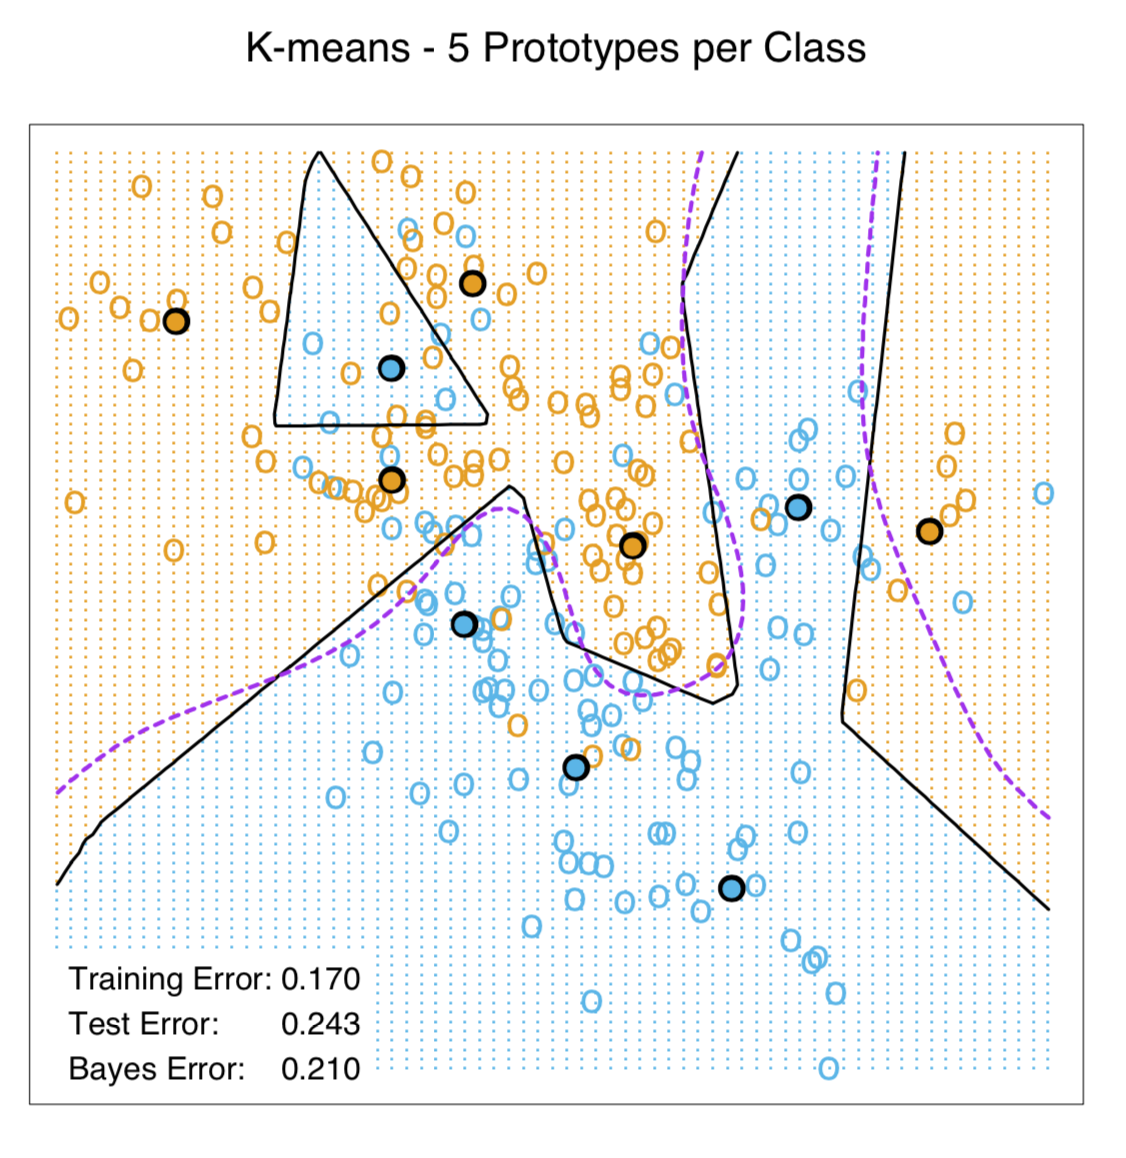
\includegraphics[width=1\linewidth]{img/kmeans}
\end{subfigure}
\hfill
\begin{subfigure}{0.49\textwidth}
\centering
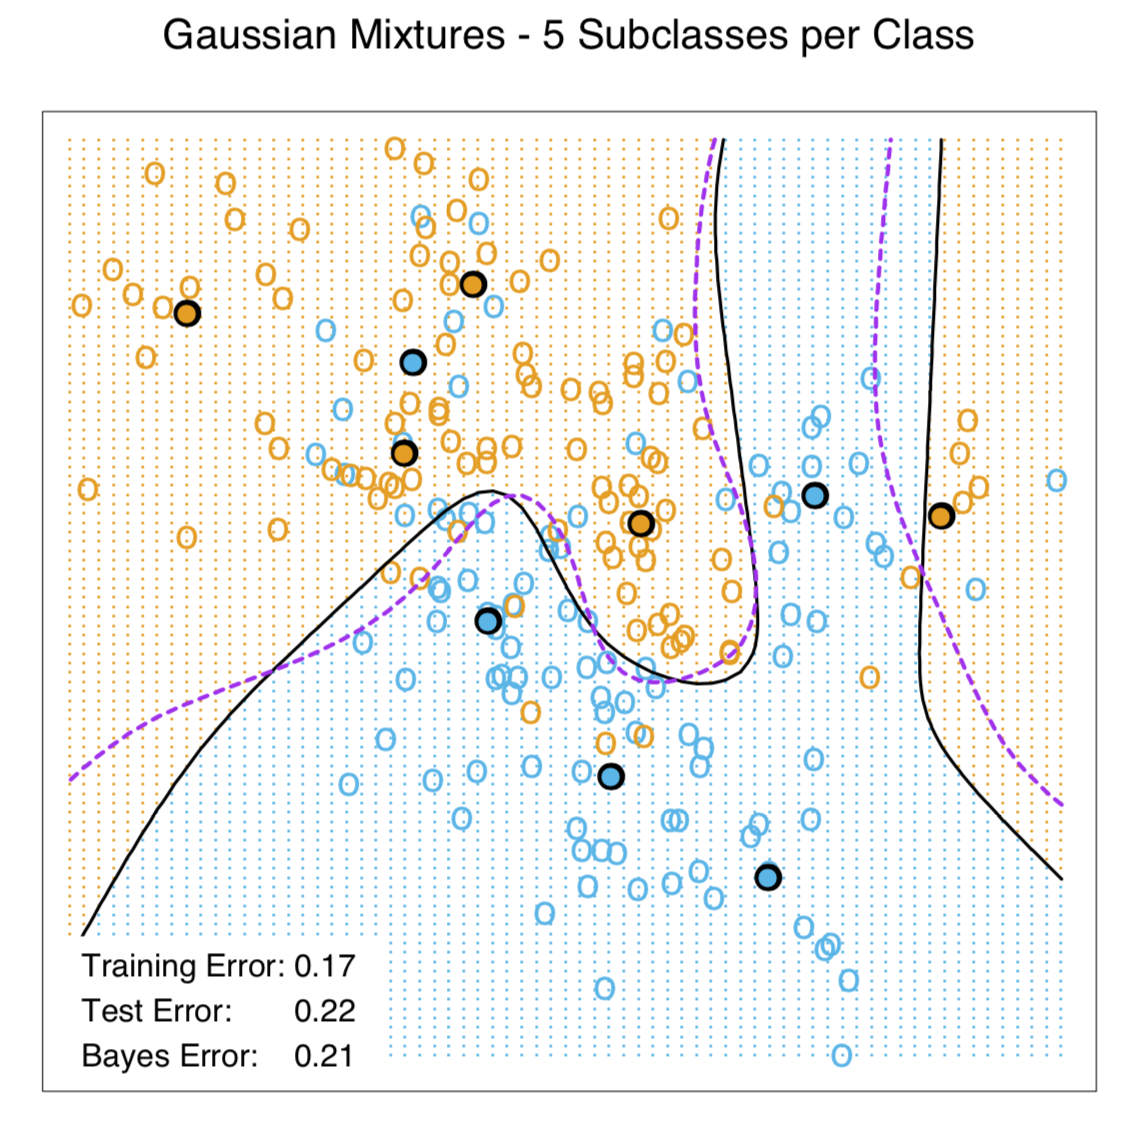
\includegraphics[width=1\linewidth]{img/GaussianMix}
\end{subfigure}
\caption{Comparison between k-means and Gaussian Mixture model with the same prototypes.}
\end{figure}

\subsection{K-nearest neighbour classifier}
These classifiers are memory-based, and require no model to be fit. Given a query point $x_0$, we find the k training points $x(r),r = 1,...,k$ closest in distance to $x_0$, and then classify using majority vote among the k-neighbors. Ties are broken at random.Typically we first standardize each of the features to have mean zero and variance 1, since it is possible that they are measured in different units. Because it uses only the training point closest to the query point, the bias of the 1-nearest-neighbor estimate is often low, but the variance is high.

\subsection{Adaptive Nearest Neighbour}
Implicit in near-neighbor classification is the assumption that the class probabilities are roughly constant in the neighborhood, and hence simple averages give good estimates.
However, in the example of \autoref{DANN} the class probabilities vary only in the horizontal direction. If we knew this, we would stretch the neighborhood in the vertical direction, as shown by the tall rectangular region. This will reduce the bias of our estimate and leave the variance the same.

\begin{figure}
\centering
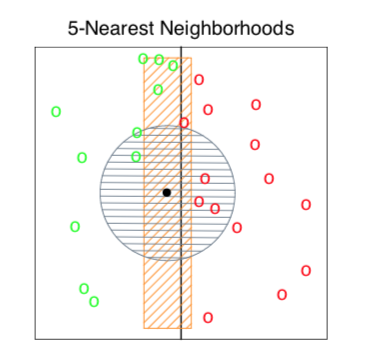
\includegraphics[scale=0.7]{img/DANN}
\caption{The points are uniform in the cube, with the vertical line sepa- rating class red and green. The vertical strip denotes the 5-nearest-neighbor region using only the horizontal coordinate to find the nearest-neighbors for the target point (solid dot). The sphere shows the 5-nearest-neighbor region using both co- ordinates, and we see in this case it has extended into the class-red region (and is dominated by the wrong class in this instance).}
\label{DANN}
\end{figure}

This suggests the idea of adapting metrics, so that the resulting neighbourhood stretch out in directions for which the class probabilities do not change much. One of these methods is the \textbf{Discriminant Adaptive Nearest-Neighbourhood (DANN)}. 
At each query point a neighborhood of say 50 points is formed, and the class distribution among the points is used to decide how to deform the neighborhood—that is, to adapt the metric. The adapted metric is then used in a nearest-neighbor rule at the query point. Thus at each query point a potentially different metric is used.

The DANN metric at a query $x_0$ is defined by:
\begin{equation}
\begin{aligned}
&D(x,x_0) = (x-x_0)^T\Sigma (x-x_0)\\
&\Sigma = \mathbf{W}^{-\frac{1}{2}} \left[ \mathbf{W}^{-\frac{1}{2}}\mathbf{B}\mathbf{W}^{-\frac{1}{2}} + \epsilon \I \right] \mathbf{W}^{-\frac{1}{2}} = \\
&\quad\quad = \mathbf{W}^{-\frac{1}{2}}\left[ \mathbf{B}^*+\epsilon\I\right] \mathbf{W}^{-\frac{1}{2}}\\
&\mathbf{W} = \sum_{k=1}^K \pi_k  \mathbf{W}_k\\
& \mathbf{B} = \sum_{k=1}^K \pi_k  (\bar{x}_k - \bar{x})(\bar{x}_k - \bar{x})^T
\end{aligned}
\end{equation}

$ \mathbf{W}$ is the pooled within-class covariance matrix and $\mathbf{B}$ is the between class covariance matrix, both computed with the $K$ nearest neighbours around $x_0$.
The formula first spheres the data with respect to $\mathbf{W}$ and then stretches the neighbourhood in the zero-eigenvalue directions of $\mathbf{B}^*$.
This makes sense, since locally the observed class means do not differ in these directions. The $\epsilon$ parameter rounds the neighborhood, from an infinite strip to an ellipsoid, to avoid using points far away from the query point. The value of $\epsilon = 1$ seems to work well in general.

\autoref{DANNConcentr} shows the resulting neighborhoods for a problem where the classes form two concentric circles. Notice how the neighborhoods stretch out orthogonally to the decision boundaries when both classes are present in the neighborhood. In the pure regions with only one class, the neighborhoods remain circular: in these cases the between matrix $\mathbf{B} = 0$, and the $\Sigma$ is the identity matrix.
\begin{figure}
\centering
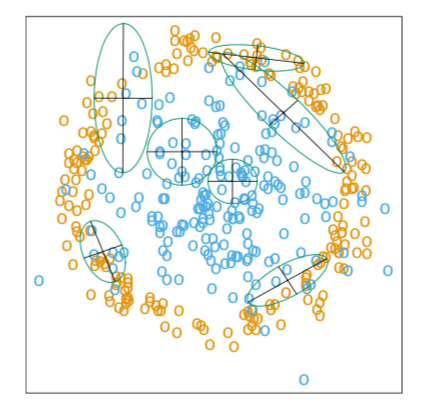
\includegraphics[scale=0.7]{img/DANNConcentr}
\caption{ Neighborhoods found by the DANN procedure, at various query points (centers of the crosses). There are two classes in the data, with one class surrounding the other. 50 nearest-neighbors were used to estimate the local metrics. Shown are the resulting metrics used to form 15-nearest-neighborhoods.}
\label{DANNConcentr}
\end{figure}

\subsubsection{Global Dimension Reduction for Nearest Neighbours}
The discriminant-adaptive nearest-neighbor method carries out local dimension reduction, that is, dimension reduction separately at each query point. In many problems we can also benefit from global dimension reduction, that is, apply a nearest-neighbor rule in some optimally chosen subspace of the original feature space.

At each training point $x_i$, the between-centroids sum of squares matrix $\mathbf{B}_i$ is computed, and then these matrices are averaged over all training points:
\begin{equation}
\bar{\mathbf{B}} = \frac{1}{N} \sum_{i=1}^N \mathbf{B}_i
\end{equation}

Let $e_1, \cdots, e_p$ be the eigenvectors  of the matrix $\mathbf{B}$ decreasingly ordered. These eigenvectors span the optimal subspaces for global subspace reduction. The rank-$L$ approximation to $\bar{\mathbf{B}}$ is:
\begin{equation}
\bar{\mathbf{B}}_L = \sum_{\ell=1}^L \theta_\ell e_\ell e_\ell^T
\end{equation}
and it solves the least squares problem
\begin{equation}
\min_{rank(\mathbf{M}) = L} \sum_{i=1}^N trace \left[ \br{\mathbf{B}_i - \mathbf{M}}^2\right]
\end{equation}
$\mathbf{B}_i$ contains information on the local discriminant subspace and the strength of discriminant in that subsapce, it can be seen as a way of finding the best approximating subspace of dimension $L$ to a series of $N$ subspaces by weighted least squares.

For example, when some eigenvalues turn out to be large (having eigenvectors nearly spanning the interesting subspace), and the remaining six are near zero,  we project the data into the leading four-dimensional subspace, and then carry out nearest neighbour classification.

\subsubsection{Computational considerations}
One drawback of nearest-neighbour is the computational load, both in finding the neighbours and storing the entire training set.

Reducing the storage requirements is difficult, and various editing and condensing procedures have been proposed. The idea is to isolate a subset of the training set that suffices for nearest-neighbour predictions, and throw away the remaining training data. Intuitively, it seems important to keep the training points that are near the decision boundaries and on the correct side of those boundaries, while some points far from the boundaries could be discarded.
The multi-edit algorithm of Devijver and Kittler (1982) divides the data cyclically into training and test sets, computing a nearest neighbour rule on the training set and deleting test points that are misclassified. The idea is to keep homogeneous clusters of training observations.

The condensing procedure of Hart (1968) goes further, trying to keep only important exterior points of these clusters. Starting with a single randomly chosen observation as the training set, each additional data item is processed one at a time, adding it to the training set only if it is misclassified by a nearest-neighbour rule computed on the current training set.

%%%%%%%%%%%%%%%%%%%%%%%%%%%%%%%%%%%%%%%%%%%%%%%%%%%%%%%%%%
%%%%%%%%------------------------------NEW SECTION------------------------------%%%%%%%%%
%%%%%%%%%%%%%%%%%%%%%%%%%%%%%%%%%%%%%%%%%%%%%%%%%%%%%%%%%%
\newpage
\section{Unsupervised learning}
In unsupervised learning one is given $N$ observations $x_1, x_N$ of a random $p$-vector $X$ having joint density $Pr(X)$. The goal is to directly infer the properties of this probability density without the help of a supervisor providing correct answers or degree of error. 

The dimension of $X$ is sometimes much higher than in supervised learning, and the properties of interest are often more complicated than simple location estimates. These factors are somewhat mitigated by the fact that $X$ represents all of the variables under consideration; one is not required to infer how the properties of $Pr(X)$ change, conditioned on the changing values of another set of variables.

In the context of unsupervised learning, there is no such direct measure of success. It is difficult to ascertain the validity of inferences drawn from the output of most unsupervised learning algorithms. One must resort to heuristic arguments not only for motivating the algorithms, as is often the case in supervised learning as well, but also for judgements as to the quality of the results. 

\subsection{Association rule}
The goal is to find joint values of the variables $X = (X_1, X_2, \cdots , X_p)$ that appear most frequently in the data base. It is mostly applied to binary-valued data $X_j = \{0,1\}$, where it is referred to as \textbf{Market basket analysis}. n this context the observations are sales transactions, such as those occurring at the checkout counter of a store. The variables represent all of the items sold in the store. For observation i, each variable $X_j$ is assigned $1$ if the item is purchased, $0$ otherwise.

More generally, the basic goal of association rule analysis is to find a collection of prototype $X$-values $v_1,\cdots,v_L$ for the feature vector $X$, such that the probability density $Pr(v_\ell)$ evaluated at each of those values is relatively large. This basically means find any kind of pattern that tells us how things go together. In this way the problem can be seen as \textbf{mode finding} or \textbf{bump hunting}.

A natural estimation of $Pr(v_\ell)$ is the number of occurrences for which $X=v_\ell$. With a large number of variables however, such observations will be to few to be reliable. The problem can be restated in another way.

Instead of seeking the values $x$ where $Pr(x)$ is large, one seeks region of the $X$-space with high probability content relative to their size or support.
\begin{definition}{\textbf{Support}}
The support $\CMcal{S_j}$ of a variable $j$is the set of all possible values for the variable.
\end{definition}
Let $\CMcal{S_j}$ represent the set of all possible values of the $j-th$ variable (its support) and let $ s_j \subseteq \CMcal{S_j}$ be a subset of these values. The modified goal can be stated as attempting to find subsets of variable values $s_1, \cdots, s_p$ such that the probability of each of the  variables is simultaneously assuming a value within its respective subset

\begin{equation}
Pr\left[ \bigcap\limits_{j = 1}^p \br{X_j \in s_j}\right]
\end{equation}
 is relatively large. $\bigcap\limits_{j = 1}^p \br{X_j \in s_j}$ is the intersection of subsets and it is called \textbf{conjunctive rule}.

\subsubsection{Market basket analysis}
For commercial databases $p\sim 10^4$, $N \sim 10^8$. In this cases many existing algorithm are not feasible and market basket analysis is applied.

Some simplifications are required: either $s_j$ consists of a single value of $X_j$ ($s_j = v_{0j}$), or it consists of the entire set of values of $X_j$ ($s_j = S_j$). So this simplifies to the problem of identifying the subset for which $s_j$ is a single value and and this  set is named $\CMcal{J} \subset \{1,\cdots,p\}$ and for each element in this subset find the corresponding value $v_{0j}$ such that:
\begin{equation}
Pr\left[ \bigcap\limits_{j \in \CMcal{J}} \br{X_j = v_{0j}}\right]
\label{dummyVarProb}
\end{equation}
is large.

One can apply the technique of dummy variables to turn \autoref{dummyVarProb} into a problem involving only binary-valued variables. Here we assume that the support $S_j$ is finite for each variable $X_j$. Specifically, a new set of variables $Z_1, \cdots, Z_K$ is created, one such variable for each of the values $v_{lj}$ attainable by each of the original variables $X_1, \cdots, X_p$. The number of dummy variables $K$ is
\begin{equation}
K = \sum_{j=1}^p |\CMcal{S}_j|
\end{equation}
where $|\CMcal{S}_j|$ is the number of distinct values attainable by $X_j$.  Each dummy variable is assigned the value $Z_k = 1$ (with $Z_k$ being associated to $v_{lj}$), if the variable with which it is associated takes on the corresponding value to which $Z_k$ is assigned (i.e., $Z_k$ is associated with $v_{lj}$; $Z_k = 1$ if  $X_j=v_{lj}$), and $Z_k = 0$ otherwise. This corresponds to find a subset of integers $\CMcal{K} \subset \{1,\cdots, K\}$ such that:

\begin{equation}
Pr\left[ \bigcap\limits_{k \in \CMcal{K}} \br{Z_k = 1}\right] = Pr\left[ \prod_{k \in \CMcal{K}} Z_k = 1\right]
\end{equation}
is large.

This is the standard formulation of the market basket problem. The set $K$ is called an \textbf{item set}. The number of variables $Z_k$ in the item set is called its "size" (note that the size is no bigger than $p$).

The estimated value of the previous expression is taken to be the fraction of observations in the database for which the conjunction is true:
\begin{equation}
\hat{Pr}\left[ \bigcap\limits_{k \in \CMcal{K}} \br{Z_k = 1}\right] = \frac{1}{N}\sum_{i=1}^N \prod_{k \in \CMcal{K}} z_{ik}
\end{equation}
where $z_{ik}$ is the value of $Z_k$ in the $i$-th case. This is called support or prevalence $T(\CMcal{K})$ if the item-set $\CMcal{K}$.

In association rule, a lower support bound $t$ is specified and one seeks all sets $\CMcal{K}_\ell$ that can be formed from the variables $Z_k$ with support in the data base greater than this lower bound $t$.

\subsubsection{Apriori algorithm}
For a given support threshold $t$ The cardinality $|\{\CMcal{K}| T(\CMcal{K}) \}|$ is relatively small. Any item set consisting of a subset of the items $\CMcal{K}$ must have support greater than or equal to that of  $\CMcal{K}$:  $\CMcal{L} \subseteq \CMcal{K} \Rightarrow T(\CMcal{L})\ge T(\CMcal{K})$.

The first pass over the data computes the support of all single-item sets. Those whose support is less than the threshold are discarded. The second pass computes the support of all item sets of size two that can be formed from pairs of the single items surviving the first pass. Each successive pass over the data considers only those item sets that can be formed by combining those that survived the previous pass with those retained from the first pass. Passes over the data continue until all candidate rules from the previous pass have support less than the specified threshold.

The items $Z_k$, $k \in K$, are partitioned into two disjoint subsets, $A \cup B = K$, and written $A\Rightarrow B$. $A$ is called antecedent and $B$ consequent.

Association rules are defined to have several properties based on the prevalence of the antecedent and consequent item sets in the data base. The support of the rule $T(A\Rightarrow B)$ is the fraction of observations in the union of the antecedent and consequent, which is just the support of the item set $K$ from which they were derived. It can be viewed as an estimate of the probability of simultaneously observing both item sets $Pr(A \text{and} B)$ in a randomly selected market basket. The "confidence" or "predictability" $C(A\Rightarrow B)$ of the rule is its support divided by the support of the antecedent:
\begin{equation}
C(A\Rightarrow B) = \frac{T(A\Rightarrow B)}{T(A)}
\end{equation}
which can be viewed as an estimate $Pr(A|B)$.

The "expected confidence" is defined as the support of the consequent $T(B$), which is an estimate of the unconditional probability $Pr(B)$. Finally, the "lift" of the rule is defined as the confidence divided by the expected confidence:
\begin{equation}
L(A\Rightarrow B) = \frac{C(A\Rightarrow B)}{T(B)}
\end{equation}
This is an estimate of the association measure $Pr(A \text{and} B)/Pr(A)Pr(B)$.

Suppose the item set $K = \{peanut butter, jelly, bread\}$ and consider the rule $\{peanut butter, jelly\} \Rightarrow \{bread\}$. A support value of $0.03$ for this rule means that peanut butter, jelly, and bread appeared together in $3\%$ of the market baskets. A confidence of $0.82$ for this rule implies that when peanut butter and jelly were purchased, $82\%$ of the time bread was also purchased. If bread appeared in $43\%$ of all market baskets then the rule $\{peanut butter, jelly\} \Rightarrow \{bread\}$ would have a lift of $1.95$.

A confidence threshold c is set, and all rules that can be formed from those item sets with confidence greater than this value:
\begin{equation}
\{ A\Rightarrow B| C(A\Rightarrow B)>c\}
\end{equation}


The output of the entire analysis is a collection of association rules (14.7) that satisfy the constraints:
\begin{equation}
T(A \Rightarrow B) >t \quad \text{and}\quad C(A \Rightarrow B)>c
\end{equation}

\subsection{Generalized association rule}
...

\subsection{Cluster Analysis}
The goal is grouping or segmenting a collection of objects into subsets or "clusters", such that those within each cluster are more closely related to one another than objects assigned to different clusters. Objects can be described by a set of measurements, or by relations to other objects. In addition, the goal is sometimes to arrange the clusters into a natural hierarchy. This involves successively grouping the clusters themselves.

A clustering method attempts to group the objects based on the definition of similarity supplied to it.

K-means clustering starts with guesses for the three cluster centers. Then it alternates the following steps until convergence:
\begin{itemize}
\item  for each data point, the closest cluster center (in Euclidean distance) is identified;
\item each cluster center is replaced by the coordinate-wise average of all data points that are closest to it.
\end{itemize}

This is a top-down procedure.

\subsubsection{Proximity Matrices and dissimilarities}
In social science experiments, participants are asked to judge by how much certain objects differ from one another. Dissimilarities can then be computed by averaging over the collection of such judgements.

This type of data can be represented by an $N \times N$ matrix $D$, where $N$ is the number of objects, and each element $d_{ii'}$ records the proximity between the $i$-th and $i'$-th objects. Most algorithms use $d_{ii}= 0$ and non negative weights.

Some algorithms require a dissimilarity matrix. Given $d_j(x_{ij}, x_{i'j}$ a dissimilarity between values of the $j$-the attribute, we define the dissimilarity between objects $i$ and $i'$ as:
\begin{equation}
D(x_i, x_{i'}) = \sum_{j=1}^p d_j (x_{ij}, x_{i'j})
\end{equation}
Most likely $d_j$ is the squared distance. For quantitative variables other common choice are the absolute error or correlation:
\begin{equation}
\rho(x_i, x_{i}) = \frac{\sum_j (x_{ij} - \bar{x}_i)(x_{i'j} - \bar{x}_i)}{\sqrt{\sum_j (x_{ij} - \bar{x}_i)^2(x_{i'j} - \bar{x}_i)^2}}
\end{equation}
\textbf{Ordinal variables} are often represented as contiguous integers. Examples are academic grades (A, B, C, D, E, F), degree of preference and so on. 
\textbf{Categorical or nominal variables} one can build a symmetric matrix with $M$ values s.t. $L_{ij}=L_{ji}\ge 0$ and $L_{ii}=0$. A popular choice is $L_{ii} = 0$.

To calculate \textbf{dissimilarity between objects} generally a weighted average is used:
\begin{equation}
D(x_i, x_{i'}) = \sum_{j=1}^p w_j d_j (x_{ij}, x_{i'j})
\end{equation}
Let us define the average dissimilarity on the $j$-th attrbute as:
\begin{equation}
\bar{d}_j = \frac{1}{N^2}\sum_{i=1}^N\sum_{i'=1}^N d_j(x_{ij}x_{i'j})
\end{equation}
We might define $w_j \sim \frac{1}{\bar{d}_j}$would give all attributes equal influence in characterizing overall dissimilarity between objects. In general, setting $w_j = \frac{1}{\bar{d}_j}$ for all attributes, irrespective of type, 
will cause each one of them to equally influence the overall dissimilarity between pairs of objects. However, if the goal is to segment the data into groups of similar objects, all attributes may not contribute equally to the (problem-dependent) notion of dissimilarity between objects.

\subsubsection{Combinatorial Algorithms}
Combinatorial algorithms work directly on the observed data with no direct reference to an underlying probability model. They assign each observation to a group or cluster without regard to a probability model describing the data. Each observation is uniquely labeled by an integer $i \in \{1,\cdots, N\}$.

A prespecified number of clusters $K<N$ is assumed.  Each observation is assigned to one and only one cluster. Given the dissimilarities between every pair of observations we want to assign each point to a cluster by the algorithm outputting a value corresponding to the cluster.

One approach is to directly specify a mathematical loss function and attempt to minimize it through some combinatorial optimization algorithm.Since the goal is to assign close points to the same cluster, a natural loss (or "energy") function would be:

\begin{equation}
W(C)  = \frac{1}{2}\sum_{k=1}^K \sum_{C(i) = k} \sum_{C(i') = k} d(x_i, x_{i'})
\end{equation}
where $C(i) = k$ is an encoder assigning someway the point $i$ to the class $k$.
This criterion characterizes the extent to which observations assigned to the same cluster tend to be close to one another.

$W(C)$ is referred to as \textbf{within-cluster point scatter} while 
\begin{equation}
B(C) =\frac{1}{2} \sum_{k=1}^K \sum_{C(i) = k} \sum_{C(i') \ne k} d(x_i, x_{i'}
\end{equation}
as the \textbf{between-cluster point scatter} and
\begin{equation}
T = \frac{1}{2} \sum_{i=1}^N \sum_{i'=1}^N d_{ii'} = W(C) + B(C) = const
\end{equation}
is the \textbf{total point scatter} which is a constant given the data. $B(C)$ tends to be large when observations assigned to different clusters are far apart.
So we have $W(C) = T - B(C) $ minimizing $W(C)$ is equivalent to maximizing $B(C)$.

Such optimization by complete enumeration is feasible only for very small data sets. The number of distinct assignments is
\begin{equation}
S(N,K) = \frac{1}{K!} \sum_{k=1}^K (-1)^{K-k} \binom{K}{k} k^N
\end{equation}
For example, $S(10, 4) = 34105$ which is still feasible, but $S(19,4) \approx 10^{10}$.  For this reason, practical clustering algorithms are able to examine only a very small fraction of all possible encoders $k = C(i)$. The goal is to identify a small subset that is likely to contain the optimal one, or at least a good suboptimal partition. Such feasible strategies are based on iterative greedy descent.

\subsubsection{K-means}
The $K$-means algorithm is one of the most popular iterative descent clustering methods. It is intended for situations in which all variables are of the quantitative type, and squared Euclidean distance.
The within-point scatter can be written as:
\begin{equation}
\begin{aligned}
&W(C) = \frac{1}{2}\sum_{k=1}^K \sum_{C(i) = k} \sum_{C(i') = k} |x_i - x_{i'}|^2= \sum_{k=1}^K N_k \sum_{C(i) = k}  |x_i - \bar{x}_{k}|^2\\
& N_k = \sum_{i=1}^N I(C(i) = k)
\end{aligned}
\end{equation}
where $\bar{x}_k$ is the mean vector associated with the $k$th-cluster. So the $N$ observations are assigned in a way such that within each cluster the average dissimilarity of the observations from the cluster mean is minimized.
\begin{algorithm}
For a given cluster assignment $C$, the total cluster variance is minimized w.r.t. $m_1, \cdots, m_K$, yielding the means of the currently assigned clusters\;
Given a current set of means the total cluster variance is minimized by assigning each observation to the closest cluster mean: $C(i) = \argmin{1\le k\le K}{|x_i-m_k|^2}$\;
Iterate the previous steps until assignment do not change.
\caption{K-means algorithm}
\end{algorithm}

\subsubsection{Gaussian Mixtures as Soft K-means Clustering}
The K-means clustering procedure is closely related to the EM algorithm for estimating a certain Gaussian mixture model. The E-step of the EM algorithm assigns "responsibilities" for each data point based in its relative density under each mixture component, while the M-step recomputes the component density parameters based on the current responsibilities. Suppose we specify K mixture components, each with a Gaussian density having scalar covariance matrix $\sigma^2\I$. Then the relative density under each mixture component is a monotone function of the Euclidean distance between the data point and the mixture center. Hence in this setup EM is a "soft" version of K-means clustering, making probabilistic (rather than deterministic) assignments of points to cluster centres. With $\sigma^2 \rightarrow 0$  the models coincide.

\subsection{Vector quantization}
Used in image processing to compress images at a cost of loss in quality. VQ breaks the image into small blocks of pixels $2 \times 2$ for example. Suppose the image is $1024 \times 1024$ pixels, then we get $512\times 512$ blocks of four pixels, i.e. a vector in $\CMcal{R}^4$. A k-means clustering algorithm is run in this space.  Each block is approximated with its closest cluster, known as codeword. The bigger $K$ the less lossy is the compression, and it is big enough we can achieve a lossless compression. The clustering process is called the encoding step, and the collection of centroids is called the codebook. To name and identify the codebook entries approximating the blocks will require $\log_2(K)$ bits per block. We also need to supply the codebook itself, which is $K \times 4$ real numbers.

\subsubsection{K-medoids}
Squared Euclidean distance places the highest influence on the largest distances. This causes the procedure to lack robustness against outliers that produce very large distances.  In the most common form, centres for each cluster are restricted to be one of the observations assigned to the cluster.
\begin{algorithm}
For a given cluster assignment C find the observation in the cluster
minimizing total distance to other points in that cluster:
\begin{equation}
i_k^* = \argmin{\{i:C(i) = k\}} \sum_{C(i')=k}D(x_i, x_{i'})
\end{equation}
Then $m_k=x_{i_k^*}$, $k=1,\cdots, K$ are the current estimates of the cluster centres\;
Given a current set of clusters centres $\{m_1, \cdots, m_K\}$ minimize the total error by assigning each observation to the closest current cluster centre:
\begin{equation}
C(i) = \argmin{1\le k\le K}{D(x_i, m_k)}
\end{equation}\;
Iterate the previous steps until the assignment do not change.
\caption{K-medoids}
\end{algorithm}
This algorithm assumes attribute data, but the approach can also be applied to data described only by proximity matrices.

\subsubsection{Number of cluster}
Suggestions range from simple random selection to a deliberate strategy based on forward stepwise assignment. At each step a new center $i_k$ is chosen to minimize the given criterion, given the centres $i_1, \cdots, i_{k-1}$ chosen at the previous steps. This continues for $K$ steps, thereby producing $K$ initial centres with which to begin the optimization algorithm.

For data segmentation $K$ is usually defined as part of the problem. For example, a company may employ $K$ sales people, and the goal is to partition a customer database into $K$ segments, one for each sales person, such that the customers assigned to each one are as similar as possible.

In other cases it must be estimated typically by examining the within-cluster dissimilarity $W_K$ as a function of the number of clusters $K$. Separate solutions are obtained for $K \in \{1, \cdots , K_{max}\}$. Generally $W_k$ decreases with increasing $K$, even when the criterion is evaluated on an independent test set.

\subsubsection{Hierarchical clustering}
Hierarchical clustering methods require the user to specify a measure of dissimilarity between (disjoint) groups of observations, based on the pairwise dissimilarities among the observations in the two groups. They produce hierarchical representations in which the clusters at each level of the hierarchy are created by merging clusters at the next lower level. At the lowest level, each cluster contains a single observation. At the highest level there is only one cluster containing all of the data.

Strategies for hierarchical clustering divide into two basic paradigms: agglomerative (bottom-up, ) and divisive (top-down).

In agglomerative methods, the pair chosen for merging consist of the two groups with the smallest intergroup dissimilarity. For divise-methods, the split is chosen to produce two new groups with the largest between-group dissimilarity. With both paradigms there are $N - 1$ levels in the hierarchy.

Recursive binary splitting/agglomeration can be represented by a rooted binary tree. 

\subsubsection{Agglomerative clustering}
Agglomerative clustering algorithms begin with every observation repre- senting a singleton cluster. At each of the $N - 1$ steps the closest two (least dissimilar) clusters are merged into a single cluster, producing one less cluster at the next higher level. Therefore, a measure of dissimilarity between two clusters (groups of observations) must be defined.

Given two groups $G$ and $H$ and two observations $i \in G$, $i' \in H$ the pairwise observation dissimilarity between these two points is $d_{ii'}$. The dissimilarity bbtw $G$ and $H$ is computed from the set of all dissimilarities.

\textbf{Single linkage} agglomerative clustering takes the intergroup dissimilarity to be that of the closest (least dissimalar) pair:
\begin{equation}
D_{SL} = \min_{i \in G, i' \in H} d_{ii'}
\end{equation}
This is often called \textbf{nearest neighbour technique}. \textbf{Complete linkage} agglomerative clustering  takes the intergroup dissimilarity to be that of the furthest pair (most dissimilar pair):
\begin{equation}
d_{CL} (G,H) = \max_{i \in G, i' \in H} d_{ii'}
\end{equation}
\textbf{Group average} clustering uses the average:
\begin{equation}
d_{GA} = \frac{1}{N_GN_H}\sum_{i \in G}\sum_{i' \in H}
\end{equation}
where $N$ are the num. observations in each group. If the data dissimilarities exhibit a strong clustering tendency, with each of the clusters being compact and well separated from others, then all three methods produce similar results.

Single linkage only requires that a single dissimilarity be small for two groups to be considered close together, irrespective of the other observation dissimilarities between the groups. It will therefore have a tendency to combine, at relatively low thresholds, observations linked by a series of close intermediate observations. This phenomenon, referred to as \textbf{chaining}, is often considered a defect of the method.

Complete linkage represents the opposite extreme. Two groups $G$ and $H$ are considered close only if all of the observations in their union are relatively similar. It will tend to produce compact clusters with small diameters.
However, it can produce clusters that violate the "closeness" property. That is, observations assigned to a cluster can be much closer to members of other clusters than they are to some members of their own cluster.
Group average clustering represents a compromise between the two extremes of single and complete linkage. It attempts to produce relatively compact clusters that are relatively far apart. However, its results depend on the numerical scale on which the observation dissimilarities are measured.
\subsubsection{Divisive clustering}
The divisive paradigm can be employed by recursively applying any of the combinatorial methods such as K-means or K-medoids , with $K = 2$, to perform the splits at each iteration.

A better approach is by Smith et. al(1965). It begins by placing all observations in a single cluster $G$. It then chooses that observation whose average dissimilarity from all the other observations is largest. This observation forms the first member of a second cluster $H$. At each successive step that observation in $G$ whose average distance from those in $H$, minus that for the remaining observations in $G$ is largest, is transferred to $H$. This continues until the corresponding difference in averages becomes negative. That is, there are no longer any observations in $G$ that are, on average, closer to those in $H$.

\subsubsection{Self-organizing maps}
...

\subsection{Principal components, curves and surfaces}
The principal components of a set of data in $\CMcal{R}^p$ provide a sequence of best linear approximations to that data, of all ranks $q \le p$. Given the observations $x_1, \cdots, x_N$, the linear approximation is:
\begin{equation}
f(\lambda) = \mu  + \mathbf{V}_q\lambda
\end{equation}
where $\mathbf{V}_q$ is a $p\times q$ matrix with $q$ orthogonal unit vectors as columns, $\lambda$ a $q$ vector of parameters and $\mu$ a location vector in $\CMcal{R}^p$. This is a $p$ hyperplane. Fitting such a model corresponds to minimize the reconstruction error:
\begin{equation}
\min_{\mu, \{\lambda_i\}, \mathbf{V}_q} \sum_{i=1}^N \| x_i -\mu - \mathbf{V}_q\lambda_u \|^2
\end{equation}
We can partially optimize to obtain:
\begin{equation}
\begin{aligned}
\hat{\mu} &= \bar{x}\\
\hat{\lambda}_i &= \mathbf{V}_q^T (x_i - \bar{x})
\end{aligned}
\end{equation}
so we must find the matrix $\mathbf{V}_q$:
\begin{equation}
\min_{\mathbf{V}_q} \sum_{i=1}^N  \| \br{x_i - \bar{x}} -\mathbf{V}_q\mathbf{V}_q^T\br{x_i - \bar{x}}\|^2
\end{equation}
For convenience we assume $\bar{x}=0$, if not true then one replaces with $\tilde{x}_i = x_i = \bar{x}$.
The matrix
\begin{equation}
\mathbf{H}_q = \mathbf{V}_q \mathbf{V}_q^T
\end{equation}
is a projection matrix so that each point $x_i$ is mapped onto its rank-$q$ reconstruction $\mathbf{H}_q x_i$, the orthogonal projection of $x_i$ spanned by the columns $\mathbf{V}_q$.

Consider the matrix $\X = \br{\x_1^T, \cdots, \x_N^T}$ of the observations and perform the singular value decomposition:
\begin{equation}
\X = \mathbf{U}\mathbf{D}\mathbf{V}^T
\end{equation}

$\mathbf{U}$ is a $N\times p$ orthogonal matrix $\mathbf{U}^T\mathbf{U}=\I_p$ whose columns $\mathbf{u}_j$ are called \textbf{left singular vectors}. $\mathbf{V}$ is a $p\times p$ orthogonal matrix ($\mathbf{V}^T\mathbf{V}=\I_p$) with columns $\mathbf{v}_j$ called the \textbf{right singular vectors}. $\mathbf{D}$ is a diagonal $p\times p$ matrix with $d_1\ge d_2\ge \cdots\ge d_p\ge 0$ known as \textbf{singular values}. 

For each rank $q$, (i.e., the chosen dimensionality on which the observations are projected), the solution $\mathbf{V}_q$  consists of the first $q$ columns of $\mathbf{V}$. The columns $\mathbf{UD}$ are called the \textbf{principal components} of $\X$. The $N$ optimal $\hat{\lambda}_i$ are given by the first $q$ principal components (the $N$ rows of the $N \times q$ matrix $\mathbf{U}_q\mathbf{D}_q$.

\autoref{SVDex} shows the one-dimensional principal component line in a $\CMcal{R}^2$ input space ($p=2$, $q=1$). For each observation point $x_i$ there is a closest point on the line given by $u_{i1}d_1v_1$ where $v_1$ is the direction of the line ($v_1$ is $p=2$ dimensional vector). $\hat{\lambda}_1=d_{i1}d_1$ measures distance along the line from the origin.

\begin{figure}
\centering
\includegraphics[scale=0.5]{img/SVD}
\caption{Example of SVD mapping of data from a $\CMcal{R}^2$ space (i.e., a plane) onto a line $\CMcal{R}$}
\label{SVDex}
\end{figure}
\subsubsection{Applications}
Principal components are a useful tool for dimension reduction and compression, for example for hand-written digits. If the inputs are $16\times 16$ images, inputs rely in  a $\CMcal{R}^{256}$ space.

\begin{figure}
\centering
\includegraphics[scale=0.5]{img/2PC}
\caption{2 Principal components analysis applied on the $3$ hand-written digits.}
\label{2PC}
\end{figure}
Consider PCA on hand-written digits of a single number, for example a $3$, and perform two principal components analysis $u_{i1}d_1$ and $u_{i2}d_2$ of each observation and calculate the quantiles $5\%, 25\%, 50\% 75\%, 95\%$ indicated by the grid in \autoref{2PC}. Red circles indicate those images close to the vertices of the grid where distance is in terms of the projected coordinates (but some weight is given to the components in the orthogonal space (?)). On the right of \autoref{2PC} the images corresponding to the red circles are shown and this allows to visualize the nature of the first two PC. $v_1$, the horizontal direction, mainly accounts for the length of lower "tail" of the "$3$", $v_2$ the vertical axis  accounts for character thickness. The parametrized model is:
\begin{equation}
\hat{f}(\lambda) = \bar{x} + \lambda_1 v_1+\lambda_2 v_2 
\end{equation}
that in terms of images is something like the one in \autoref{modelImage}.


\begin{figure}
\centering
\includegraphics[scale=0.7]{img/modelImage}
\caption{Equivalence of the parametrized model using image representation.}
\label{modelImage}
\end{figure}
Although there are a possible 256 principal components, approximately 50 account for 90\% of the variation in the threes, 12 account for 63\%.

A relatively small subset of the principal components serve as excellent lower-dimensional features for representing the high-dimensional data.

The same technique, with some further calculations, can be applied to digital signature.

\subsubsection{Prinipal curves and surfaces}
Principal curves generalize the concept of the principal component line to obtain smoother curves. 

Let $f(\lambda)$ be a parametrized smooth curve in $\CMcal{R}^p$. It is a vector function of with $p$ coordinates, each a smooth function of the single parameter $\lambda$. For example $\lambda$ can be chosen to be the arc-length along the curve from a fixed origin. For each data value $x$, let $\lambda_f(x)$ define the closest point on the curve to $x$. Then $f(\lambda)$ is called a principal component curve for the distribution of the random vector $X$ if:
\begin{equation}
f(\lambda) = \E\br{X|\lambda_f(X) = \lambda}
\end{equation}
So $f(\lambda)$ is the average of all data points that project to it (\textbf{self-consistency} property). Although in practice, continuous multivariate distributes have infinitely many principal curves (Duchamp and Stuetzle, 1996), we are interested mainly in the smooth ones.

A principal curve is defined by its coordinate functions: $f(\lambda) =$ $[ f_1(\lambda), f_p(\lambda)]$ and let $X^T = (X_1, \cdots, X_p)$. Consider the following alternate steps:
\begin{equation}
\begin{aligned}
&1) \quad \hat{f}_j(\lambda)\leftarrow \E \br{X_j|\lambda(X) = \lambda}; \quad j=1,\cdots, p\\
&2) \quad \hat{\lambda}_f(x) \leftarrow \argmin{\lambda'}{\|x -\hat{f}(\lambda')\|^2}
\end{aligned}
\end{equation}
In the first $\lambda$ is fixed and it enforces the self-consistency requirement. In the second the curve is fixed and it finds the closest point on the curve to each data point.

With finite data, the principal curve algorithm starts with the linear principal component, and iterates the two steps until convergence.
A scatterplot smoother is used to estimate the conditional expectations in the frist step by smoothing each $X_j$ as a function of the arc-length $\lambda(X)$, and the projection in the second step is done for each of the observed data points. Proving convergence in general is difficult, but one can show that if a linear least squares fit is used for the scatterplot smoothing, then the procedure converges to the first linear principal component, and is equivalent to the power method for finding the largest eigenvector of a matrix.

Principal surfaces have exactly the same form as principal curves, but are of higher dimension. The mostly commonly used is the two-dimensional principal surface, with coordinate functions
\begin{equation}
f(\lambda_1, \lambda_2) = \left[ f_1(\lambda_1, \lambda_2), \cdots, f_p(\lambda_1, \lambda_2)\right]
\end{equation}
Principal surfaces of dimension greater than two are rarely used, since the visualization aspect is less attractive, as is smoothing in high dimensions.

\subsubsection{Spectral Clustering}
Traditional clustering methods like K-means use a spherical or elliptical metric to group data points. Hence they will not work well when the clusters are non-convex, such as the concentric circles.

Spectral clustering solves this problem by firstly building a $N\times N$ matrix of pairwise similarities $s_{ij}\ge 0$ between all observation pairs.We represent the observations in an undirected similarity graph $G = \left\langle V, E\right\rangle$. The $N$ vertices $v_i$ are the observations and pairs of vertices are connected by an edge if their similarity is positive or exceeds some threshold. Edges are weighted by $s_{ij}$.

Clustering now is a graph-partition problem where we identify connected components with clusters. We  want to partition the graph such that edges between different groups have low weight and within a group have high weight.

Consider $N$ points $x_i \in \CMcal{R}^p$ and let $d_{ij}$ be the Euclidean distance between $x_i$ and $x_j$. We will use as similarity matrix the radial-kernel matrix:
\begin{equation}
s_{ij} = \e^{-\frac{d_{ij}^2}{c}}
\end{equation}
where $c >0$ is a scale parameter. A popular way to define the similarity matrix is the \textbf{mutual K-nearest-neighbour graph}. Define $\mathcal{N}_k$ the symmetric set of nearby pairs of points: a pair $(i,j)$ is in $\mathcal{N}_k$ if $i$ is in the $K$-neighbourhood of $j$ or viceversa. Then we connect all NN and give them edge-weight $w_{ij} = s_{ij}$, otherwise the weight is $0$.
Alternatively, a fully connected graph includes all pairwise edges with weights $w_{ij} = s_{ij}$ , and the local behaviour is controlled by the scale parameter $c$.
The matrix $\mathbf{W} = \{w_{ij}\}$ is called \textbf{adjacency matrix}; the \textbf{degree of vertex $i$} is:
\begin{equation}
g_i = \sum_j w_{ij}
\end{equation}
Let $\mathbf{G}$ be a diagonal matrix of $d_{ij}$. The \textbf{unnormalized graph Laplacian} is
\begin{equation}
\mathbf{L} = \mathbf{G} -\mathbf{W}
\end{equation}
Spectral clustering finds the $m$ eigenvectors $\mathbf{Z}_{N\times m}$ corresponding to the $m$ smallest eigenvalues of $\mathbf{G}$.  Using a standard method like $K$-means, we then cluster the rows of $\mathbf{Z}$ to yield a clustering of the original data points.

Spectral clustering works because for any vector $\mathbb{f}$:
\begin{equation}
\mathbb{f}^T\mathbb{Lf}= \sum_{i=1}^Ng_i f_i^2 -\sum_{i=1}^N\sum_{j=1}^N f_i f_j w_{ij} = \frac{1}{2}\sum_{i=1}^N\sum_{j=1}^N  w_{ij}(f_i -f_j)^2 
\end{equation}
A small value of $\mathbb{f}^T\mathbb{Lf}$ will be achieved for coordinates that are close together.
$\mathbb{1}^T\mathbb{L1}=0$ for any graph: the trivial constant vector corresponding to the $0$ eigenvalue. If the graph is connected $\mathbb{1}^T\mathbb{L1}$ is the only $0$ eigenvector.

With $m$ connected components, the nodes can be reordered so that $L$ is block diagonal with a block for each connected component. Then $L$ has $m$ eigenvectors of eigenvalue $0$, and the eigenspace of eigenvalue $0$ is spanned by the indicator vectors of the connected components. In practice one has strong and weak connections, so $0$ eigenvalues are approximated by small eigenvalues.

Spectral clustering is an interesting approach for finding non-convex clusters. 
\subsubsection{Kernel Principal components  (kernel-PCA or kPCA)}
\label{KPCA}
Support Vector Machines Kernel trick maps instances into a very high-dimensional space (called the feature space), enabling non-linear classification and regression. Recall that a linear decision boundary in the high-dimensional feature space corresponds to a complex nonlinear decision boundary in the original space.
It turns out that the same trick can be applied to PCA, making it possible to perform complex non-linear projections for dimensionality reduction. Application of a kernel means expanding the features-space by non-linear transformation. On this new higher dimensional space we can apply PCA.

Let $\phi(\dot)$ be a non-linear transformation mapping data from the input space $\CMcal{X}$ to some feature space $\CMcal{H}$. Then, the problem is the same of \autoref{PCAmaxVar}, the only difference is that the covariance matrix is the one calculated in the feature space, not in the input space. Now $\psi_\ell$ lie in the span of the mapped data, with the coefficient given by the $l-th$ eigenvector.
\begin{equation}
\lambda_\ell\psi_\ell = \frac{1}{N}\sum_{i=1}^n \langle \phi(\x_i), \psi_\ell\rangle \phi(\x_i)
\end{equation}

As in \autoref{PCALinComb} we can express the principal components as a linear combination, in this case not in terms of input vectors but in terms of feature vectors:
\begin{equation}
\psi_\ell  = \sum_{i=1}^n \alpha_{i\ell} \phi(\x_i)
\end{equation}
and substituting into the previous equation:
\begin{equation}
\begin{aligned}
\lambda_\ell \psi_\ell  = \lambda_\ell \sum_{i=1}^n \alpha_{i\ell} \phi(\x_i) &= 
\frac{1}{N}\sum_{i=1}^n \langle \phi(\x_i), \sum_{i=1}^n \alpha_{i\ell} \phi(\x_i)
\rangle \phi(\x_i)\Rightarrow\\
\lambda_\ell \sum_{i=1}^n \alpha_{i\ell} \phi(\x_i) &= \frac{1}{N}\sum_{i=1}^n \phi(\x_i)\langle \phi(\x_i), \sum_{i=1}^n \alpha_{i\ell} \phi(\x_i)
\rangle \Rightarrow\\
\Rightarrow \lambda_\ell \sum_{i=1}^n \alpha_{i\ell} \phi(\x_i) &= 
\frac{1}{N}\sum_{i=1}^n \phi(\x_i) \phi(\x_i)^T \sum_{j=1}^n \alpha_{j\ell} \phi(\x_j)  \Rightarrow
\end{aligned}
\end{equation}
The key step is now to express this in terms of the kernel function $k(\x_i , \x_j ) =
\phi(\x_n)^T\phi(\x_m )$, which we do by multiplying both sides by $\phi(\x_p)^T$ to give
\begin{equation}
\begin{aligned}
 \lambda_\ell \sum_{i=1}^n \alpha_{i\ell} \phi(\x_p)^T\phi(\x_i) &= 
\frac{1}{N}\sum_{i=1}^n \phi(\x_p)^T\phi(\x_i)  \sum_{j=1}^n \alpha_{j\ell} \phi(\x_i)^T\phi(\x_j)\Rightarrow\\
\Rightarrow  \lambda_\ell \sum_{i=1}^n \alpha_{i\ell} k(\x_p,\x_i) &= 
\frac{1}{N}\sum_{i=1}^n k(\x_p,\x_i)  \sum_{j=1}^n \alpha_{j\ell} k(\x_i,\x_j)
\end{aligned}
\end{equation}
This can be rewritten in matrix notationas
\begin{equation}
\mathbf{K}^2\mathbf{\alpha}_i = \lambda_i N  \mathbf{K} \mathbf{\alpha}_i
\end{equation}
where $\mathbf{\alpha}_i$ is a N-dimensional column vector with elements $\alpha_{\ell i}$ and $K$ is the \ti{Gram matrix} with entries $\langle \phi(\x_i), \phi(\x_j)\rangle$.

One can find solutions for $\mathbf{\alpha}_i$ by solving the following eigenvalue problem:
\begin{equation}
\mathbf{K\alpha}_\ell = \lambda_\ell N\mathbf{\alpha}_i
\end{equation}
So the expansions require only the inner products, without the need to know exactly the mapping function.

In \autoref{SVDEigenDec} we have seen how to compute the matrix $Z=UD$.
If $X$ is not centred:
\begin{equation}
\begin{aligned}
\tilde{X} &= \br{I - M}X\\
M &= \frac{1}{N}\mathbf{1}\mathbf{1}^T
\end{aligned}
\end{equation}
where $M$ is mean operator. Thus, we compute the eigenvectors of $\br{I-M}K\br{I-M}$:
\begin{equation}
\begin{aligned}
\tilde{K} &= \tilde{X}\tilde{X}^T = (I-M)XX^T(I-M)^T = (I-M)K(I-M) = U\Sigma^2U^T\\
\tilde{K} &= Q\Lambda Q^{-1}
\end{aligned}
\end{equation}

Kernel PCA interprets the kernel matrix $K = {K(xi,xi')}$ as an inner-product matrix of the implicit features $\langle\Phi(x_i ), \Phi(x_i')\rangle$ and finding its eigenvectors. 
The elements of the $m$-th component $z_m$ ($m$-th column of $Z$) can be written (up to centering) as $z_{im} = \sum^N_{j=1} \alpha_{jm}K(x_i, x_j )$, where $\alpha_{jm} = u_{jm}/d_m$.

\subsubsection{Sparse Principal components}
...
\subsection{The pre-image problem}
The kernel trick exploits the fact that a great number of data processing techniques do not depend explicitly on the data itself, but rather on a similarity measure between them and one of these measures is the inner product. In the kernel trick, the the inner product is replaced with a reproducing kernel (i.e.,  a positive definite symmetric function). The kernel is a non-linear transformation that maps input data onto a feature space: applying the kernel in the input space is equivalent to applying the inner product in this new space as a similarity measure. The advantage is that the resulting non-linear algorithms show significant performance improvements while keeping the same computational complexity.

The reverse transformation from the feature space back to the input space is called \tb{reverse mapping} and is important in kernel PCA for signal and image processing. Unfortunately, \tb{the reverse mapping generally does not exist} and only most elements in the feature space, including the equivalent of denoised signals, do not have a valid pre-image in the input-space. \tb{The pre-image problem consists of finding an approximate solution} by identifying data in the input space based on their corresponding features that are mapped close enough to desired data in the feature space. The pre-image problem is essentially a dimensionality reduction problem.

Most  well-known statistical linear techniques can be formulated as inner product between pairs of data. Thus, applying any non-linear transformation to the data can only impact the values of the resulting inner products. Therefore one does not need to compute such transformation explicitly but needs only to replace the inner product operator with an appropriate kernel, i.e., a \tb{symmetric hermitian function} \autoref{Hermitian} (with symmetric meaning $k(x,y) = k(y,x)$. The only restriction is that the latter defines an inner product in some space. A sufficient condition for this is given by t e\tb{Mercer's theorem} \autoref{} which states that any continuous positive definite function on $\CMcal{X}$ can be expressed as an inner product in some space.

Furthermore, Moore-Aronszajn  theorem states that to any positive semidefinite kernel $k$ it corresponds  a unique reproducing kernel Hilbert space (rkHs)  whose inner product $\langle\cdot \rangle$ usually called reproducing kernel is $k$ itself.

A rkHs is a Hilbert space of functions for which point evaluations are bounded, and where the existence and uniqueness of the reproducing kernel is guaranteed by the Riesz representation theorem. In fact, let $\CMcal{H}$ be a Hilbert space of functions defined on some compact $\CMcal{X}$, for which the evaluation $\psi(x)$ of the function $\psi \in H$ is bounded for all $x \in \CMcal{X}$ . By this theorem, there exists a unique function $\psi(x) \in \CMcal{H}$ such as $\psi(x) = \langle\psi,\phi(x)\rangle_\CMcal{H}$. This function has the following property:
\begin{equation}
\label{EqProd}
\CMcal{k}(\x_i, \x_j) = \langle \phi(\x_i, \x_j) \rangle_\CMcal{H}
\end{equation}
Distances can be evaluated using the kernel trick:
\begin{equation}
\begin{aligned}
\| \phi(\x_i) - \phi(\x_j) \|^2_\CMcal{H} &= \langle \phi(\x_i)- \phi(\x_j),  \phi(\x_i)- \phi(\x_j)\rangle_\CMcal{H}  =\\
&=\CMcal{k}(\x_i, \x_i)- 2 \CMcal{k}(\x_i, \x_j)+\CMcal{k}(\x_j, \x_j)
\end{aligned}
\end{equation}

Most of the kernels can be divided into two groups:
\begin{itemize}
\item projective kernels are functions of inner product (for example the polynomial kernel);
\item radial kernels or isotropic kernels are functions of distance (for example the Gaussian kernel).
\end{itemize}
These kernels map the data onto a higher dimensional space, even infinite in the case of the Gaussian kernel.
\begin{theorem}{\tb{Representer theorem}}
For any function $\psi \in CMcal{H}$ minimizing a regularized cost function in the form of
\begin{equation}
\sum_{i=1}^n f\br{y_i, \psi(\x_i)} + \eta g\br{\|\psi\|^2_\CMcal{H}}
\end{equation}
with $f(\cdot)$ some loss function and $g(\cdot)$ a strictly monotonic increasing function on $CMcal{R}_{+}$ can be written as an expansion in terms of available data:
\begin{equation}
\psi = \sum_{i=1}^n \alpha_i \phi(\x_i)
\end{equation} 
\end{theorem}
So even in an infinite rkHs, one only needs to work in the subspace spanned by the $n$ images of the training data.

\subsubsection{Solving the pre-image problem}
A problem is ill-posed if at least one of the following conditions is violated:
\begin{itemize}
\item a solution exist;
\item it is unique 
\item it depends continuously on the data.
\end{itemize}
Identifying the pre-image problem is typically an ill-posed problem due to the higher dimensionality of the feature space. As so, many elements might not have a pre-image in the input space and if it exists it might not be unique. The goal becomes to look for an approximate solution whose map is as close as possible.

The pre-image problem can be seen as 
\begin{equation}
x^* = \argmin{\x \in \CMcal{X}} \left| \sum_{i=1}^n \alpha_i \phi(\x_i) - \phi(\x)\right|^2_{\CMcal{H}}
\end{equation}
Using equation \autoref{EqProd}:
\begin{equation}
\label{MinFunct}
x^* = \argmin{\x \in \CMcal{X}} \CMcal{k}(\x,\x) -2 \sum_{i=1}^n \alpha_i \CMcal{k}(\x,\x_i) + \br{\sum_{i=1}^n \alpha_i \CMcal{k}(\x_i,\x_i)}^2
\end{equation}
where the last term can be discarded because it does not depend on $\x$. This is equivalent to the minimization of the distance.

\subsubsection{Exact pre-image}
Suppose there exists an exact pre-image $\psi$, i.e., $x^*$ such that $\phi(x^*) = \psi$. Then, the minimization problem is equivalent to finding the pre-image. The pre-image can be computed when the kernel is an invertible function of $\langle \x_i \x_j \rangle$, such as some projective kernels including odd degree polynomial kernel and the sigmoid kernel. Let $h: \CMcal{R}\rightarrow \CMcal{R}$ defines the inverse function such that $h\br{k(\x_i, \x_j)} = \langle\x_i, \x_j \rangle$. Given an orthonormal base in the input space $\{e_1, e_2, \cdots\}$, every $\x \in \CMcal{X}$ can be written as 
\begin{equation}
\x = \sum_{j=1}^N\langle e_j , \x\rangle e_j = \sum_{j=1}^N h\br{k(e_j, \x)} e_j
\end{equation}
So, the exact pre-image $x^*$ of $\psi = \phi(x^*)$ can be expanded as 
\begin{equation}
\x^* =\sum_{j=1}^N h\br{\sum_{i=1}^n\alpha_i k(e_j, \x_i)} e_j
\end{equation}
Likewise, when the kernel is an invertible function of the distance, such as radial kernels, a similar expression can be derived $4 \langle \x^*, e_j \rangle = \| \x^* + e_j \|^2 -\| \x^* + e_j \|^2 $.

Unfortunately for a large class of kernels the pre-image does not exist. The following are approximate solutions.

\subsubsection{Gradient descent techniques}
It is an iterative procedure where the current guess $\x^*_t$ is updated by taking a step in the opposite direction of the gradient of the objective function:
\begin{equation}
\x^*_{t+1} = \x^*_t - \eta_t \nabla_\x J(\x_t^*)
\end{equation}
where $\eta_t$ is a step size parameter. As an alternative to the gradient descent, one may use more sophisticated techniques such as the Newton's method (\autoref{NewtonsMethod}). Unfortunately, the objective function is non-linear and non-convex, so the procedure must be run many times with several different starting values to avoid local minima solutions.

\subsection{Fixed point iteration method}
For most kernels, the expression in \autoref{MinFunct} has a closed-form expression. By setting this expression to $0$, this greatly simplifies the optimization scheme resulting into a fixed-point iterative technique. Taking for example the Gaussian kernel the objective function becomes:
\begin{equation}
\Xi(\x) = -2 \sum_{i=1}^n \alpha_i e^{-\frac{\|\x-\x_i\|^2}{2\sigma^2}}
\end{equation}
and its gradient
\begin{equation}
\nabla_\x\Xi(\x) = -\frac{2}{\sigma^2} \sum_{i=1}^n \alpha_i e^{-\frac{\|\x-\x_i\|^2}{2\sigma^2}}(\x - \x_i)
\end{equation}
We get the pre-image setting this gradient to $0$:
\begin{equation}
x^*_{t+1} = \frac{\sum_{i=1}^n \alpha_i k(\x^*_t,\x_i)\x_i}{ \sum_{i=1}^n \alpha_i k(\x^*_t,\x_i)}
\end{equation}
with $k(\x^*_t,\x_i)= e^{-\frac{\|\x_t^*-\x_i\|^2}{2\sigma^2}}$. Instead for the polynomial kernel with degree $p$:
\begin{equation}
x^*_{t+1} =\sum_{i=1}^n   \alpha_i\br{\frac{  \langle\x^*_t,\x_i\rangle+c}{\langle\x^*_t,\x^*_t\rangle+c}}^{p-1}\x_i
\end{equation}

Such an iterative method still suffers from local minima and tends to be unstable, for example when the denominator goes to $0$. However, regularized solutions exist.

An interesting fact is that the solution lies in the span of available data, taking the form $\x^* = \sum_{i=1}^n \beta_i \x_i$. So the search space is controlled as opposed to the gradient descent which explores the entire space.

\subsubsection{Learning pre-image map}
Even a learning machine cab be constructed and trained on the elements from the feature space and estimated (target points) on the input space points. We seek a function $\Gamma^*\br{\phi(\x_i)} = \x_i$. The function must be defined on a vector space. Also, one can decompose the function in order to have functions outputting a single scalar output for every dimension in $\CMcal{X}$: 
\begin{equation}
\begin{aligned}
\Gamma^* &= \{\Gamma^*_1, \Gamma^*_2, \cdots, \Gamma^*_{dim{\CMcal{X}}}\}\\
\Gamma^*_m&: \CMcal{R}^k \Rightarrow \CMcal{R}
\end{aligned}
\end{equation}
Each of these functions is obtained by solving the optimization problem:
\begin{equation}
 \Gamma^*_m = \argmin{\Gamma}{\sum_{i=1}^n f\br{\left[\x_i\right], \Gamma(\psi)}+\eta g\br{\||Gamma\|^2}}
\end{equation}
where $f$ is the loss function. For example by taking the distance as the loss-function:
\begin{equation}
 \Gamma^*_m = \argmin{\Gamma}{\sum_{i=1}^n \|\left[\x_i\right]_m - \Gamma\br{\psi}\|^2+\eta g\br{\||Gamma\|^2}}
\end{equation}
This optimization problem can be solve by matrix inversion.

\subsubsection{Multidimensional scaling (MDS)}
MDS techniques embed data in a low-dimensional space by pairwise distances. In the rkHs the distance is 
\begin{equation}
\label{dist}
\delta_i = \|\psi- \phi(\x_i)\|_\CMcal{H}
\end{equation}
 and in the input space it is $\|\x^* - \x_i\|$. Ideally, the distances are preserved: 
 \begin{equation}
 \label{distEquality}
 \|\psi- \phi(\x_i)\|_\CMcal{H}^2 = \|\x^* - \x_i\|^2
 \end{equation}.
If $\psi = \phi(\x^*)$, then $\x^* = \x_i$. One way to solve this is to minimize the mean square error between these distances:
\begin{equation}
\x^* = \argmin{\x}{\sum_{i=1}^n \left| \|\x-\x_i\|^2 - \|\psi-\phi(\x_i) \|_\CMcal{H}^2 \right|}^2
\end{equation}
To solve this optimization problem, a fixed-point iteration method can be used by setting the gradient to $0$:
\begin{equation}
\x^* = \frac{\sum_{i=1}^n \br{\|\x^* - \x_i\|^2 = \delta_i^2}\x_i}{\sum_{i=1}^n \br{\|\x^* - \x_i\|^2 = \delta_i^2}}
\end{equation}
Another approach to solve this problem is to consider separately the identities \autoref{distEquality} recalling the definition \autoref{dist} and solving $n$:
 equations:
\begin{equation}
2\langle \x^*, \x_i\rangle=\langle \x^*, \x^*\rangle +\langle \x_i,  \x_i\rangle-\delta_i^2
\end{equation}
$\langle \x^*, \x^*\rangle $ can be identified in the case of centred data by taking the average of both sides:
\begin{equation}
\langle \x^*, \x^*\rangle  = \frac{1}{n}  \sum_{i=1}^n\br{\delta_i^2- \langle \x_i, \x_i\rangle }
\end{equation}
Let $\epsilon$ be the vector having entries equal to $\frac{1}{n}\sum_{i=1}^n\br{\delta_i^2-\langle \x_i, \x_i\rangle }$, then:
\begin{equation}
\begin{aligned}
2\X^T\x^* &= diag{\X^T \X} - \left[\delta_1^2, \delta_2^2, \cdots, \delta_n^2\right]^T+\epsilon\\
\Rightarrow \x^* &= \frac{1}{2}\br{\X\X^T}^{-1}\X\br{diag{\X^T \X} - \left[\delta_1^2, \delta_2^2, \cdots, \delta_n^2\right]^T+\cancel{\epsilon}}
\end{aligned}
\end{equation}
where the term $\br{\X\X^T}^{-1}\X\epsilon$ goes to $0$ thanks to the assumption of centred data.

To keep this technique tractable in practice, only a certain neighbourhood is considered in the pre-image estimation.
\subsubsection{Conformal map approach}
One may also propose a pre-image method to preserve the product measures, which also preserves the angular measures since  $\x_i^T \x_j/\br{\|\x_i\|\|\x_j\|}$ defines the cosine of the angle.

A coordinate system oin the rkHs is constructed with an isometry with respect to the input space. The model is not coupled with any constraint on the coordinate functions as opposed to the orthogonality constraint between the functions in the kernel PCA. 

Each of the $n$-coordinate functions can be rewritten as a linear expansion of the available imagesL $\Phi_\ell = \sum_{i=1}^n \theta_{\ell, i}\phi(\x_i)$, with unknown weights. Rearranging:
\begin{equation}
\mathbf{\Phi}_{\x_i} = \left[ \langle \Phi_1, \phi(\x_i)\rangle,  \langle \Phi_w, \phi(\x_i)\rangle \cdots\right]
\end{equation}
Preservation of the inner products yields:
\begin{equation}
\mathbf{\Phi}_{\x_i}^T\mathbf{\Phi}_{\x_i}= \x_i^T\x_j
\end{equation}
This can be minimized by minimizing the fitness error:
\begin{equation}
\min_{\Psi_1, \cdots, \Psi_n}{\sum_{i,j=1}^n \|\x_i^T\x_j - \Psi_{\x_i}^T\Psi_{\x_j}\|^2 + \eta \sum_{\ell=1}^n \|\Psi_\ell\|^2_{\CMcal{H}}}
\end{equation}
where the second term is the regularization term. Rewritten in matrix form, it becomes:
\begin{equation}
\min_{\Theta} \frac{1}{2}\sum_{i,j=1}^n \|\X^T\X - \mathbf{K\Theta^T\Theta K}\|^2_F + \eta tr\br{\mathbf{\Theta^T\Theta K}}
\end{equation}
where $\|\cdot\|_F$ is the Frobenius norm, i.e., the root of sum of squared (absolute) values of all its elements: $\|M\|^2_F=tr(M^TM)$. By taking the derivative of this expression with respect to $\Theta^T\Theta$ one obtains
\begin{equation}
\mathbf{\Theta^T\Theta = K^{-1}\br{X^TX-\eta K^{-1}}K^{-1}}
\end{equation}

Now one can determine the pre-image of $\psi = \sum_{i=1}^n\alpha_i \phi(\x_i)$. Given the system of coordinates $\{\Psi_\ell\}$:
\begin{equation}
\langle \psi, \Psi_\ell\rangle_\CMcal{H} = \sum_{i,j=1}^n \theta_{\ell,i}\alpha_j k(\x_i, \x_j)
\end{equation}

By preserving the inner products in both spaces, ideally the model can be extended to $\phi$ resulting into 
\begin{equation}
\X^T\x^* = \mathbf{K\Theta^T\Theta K\alpha}
\end{equation}
and using the previous expression:
\begin{equation}
\x^* = \br{\X\X^T}^{-1}\X\br{\X^T\X -\eta K^{-1}}\alpha,
\end{equation}
independently from the kernel type.


\subsection{Non-negative matrix factorization}
It assumes non-negative data, i.e. images. Given $\X \in \CMcal{R}^{N\times p}$, it can be approximated with
\begin{equation}
\X \sim \mathbf{W}\mathbf{H}
\end{equation}
where $\mathbf{W} \in \CMcal{R}^{N\times r}$ and $\mathbf{H} \in \CMcal{R}^{r\times p}$, $r\le max(N,p)$. We assume $x_{ij}, w_{ik}, h_{kj}\ge 0$. $\mathbf{W}$ and $\mathbf{H}$ are found by maximizing
\begin{equation}
L(\mathbf{W}, \mathbf{H}) = \sum_{i=1}^N\sum_{j=1}^p \left[ x_{ij}\log(\mathbf{WH}_{ij}) - \mathbf{WH}_{ij} \right]
\end{equation}

This is the log-likelihood from a model in which $x_{ij}$ has a Poisson distribution with mean $(\mathbf{WH})_ij$ -quite reasonable for positive data.

The following alternating algorithm (Lee and Seung, 2001) converges to a local maximum of $\mathbf{WH}$:
\begin{equation}
\begin{aligned}
w_{ik} &\leftarrow w_{ik}\frac{\sum_{j=1}^p \frac{h_{kj} x_{ij}}{\br{\mathbf{WH}}_{ij}}}{\sum_{j=1}^p h_{kj}}\\
h_{kj} &\leftarrow  h_{kj}\frac{\sum_{i=1}^p  \frac{w_{ik}x_{ij}}{\br{\mathbf{WH}}_{ij}}} {\sum_{j=1}^p h_{kj}}
\end{aligned}
\end{equation}

Unlike VQ and PCA, NMF learns to represent faces with a set of basis images resembling parts of faces.
Donoho and Stodden (2004) point out a potentially serious problem with non-negative matrix factorization. Even in situations where $X = \mathbf{WH}$ holds exactly, the decomposition may not be unique.

For example, data points in \autoref{nonUnique} lie in$ p = 2$ dimensions, and there is "open space" between the data and the coordinate axes. We can choose the basis vectors $h_1$ and $h_2$ anywhere in this open space, and represent each data point exactly with a nonnegative linear combination of these vectors. This non-uniqueness means that the solution found by the above algorithm depends on the starting values, and it would seem to hamper the interpretability of the factorization.
\begin{figure}
\centering
\includegraphics[scale=0.4]{img/NonUniqueness}
\caption{Any choice of the basis vectors h1 and h2 in the open space between the coordinate axes and data, gives an exact reconstruction of the data.}
\label{nonUnique}
\end{figure}

\subsubsection{Archetypal Analysis}
...

\subsection{Independent component analysis and Exploratory Projection Pursuit}
Multivariate data are often viewed as multiple indirect measurements arising from an underlying source. Variables that cannot be directly observed are called \textbf{latent variables}. Example are psychological IQ tests: answers are the multivariate variables (data) and the intelligence, is the latent variable we want to measure and that generated those data. The same for the EEG brain scans to measure neuronal activity: electromagnetic signals are measured by sensors placed at different points. Other examples exist.

\subsubsection{Latent variables and Factor analysis}
Factor analysis is a statistical technique that aims to find latent sources mostly exploiting Gaussian distributions.
Consider the SVD:
\begin{equation}
\begin{aligned}
\X &= \mathbf{UDV}^T\\
\mathbf{S} &= \sqrt{N}\mathbf{U}\\
\mathbf{A}^T = \frac{\mathbf{DV}^T}{\sqrt{N}}\\
\Rightarrow \X = \mathbf{SA}^T
\end{aligned}
\end{equation}
and hence each of the columns of $\X$ is a linear combination of the columns of $\mathbf{S}$. Now since $\mathbf{U}$ is orthogonal, and assuming as before that the columns of $\X$ (and hence $\mathbf{U}$) each have mean zero, this implies that the columns of $\mathbf{S}$ have zero mean, are uncorrelated and have unit variance.

However this representation is not unique: given the orthogonal matrix $\mathbf{R}$: $\X = \mathbf{AR^TRS}$.  It is therefore impossible to identify any particular latent variables as unique underlying sources.

With $q<p$ the classical factor analysis is $X = AS + \epsilon$. Here $\mathbf{S}$ is a vector of $q < p$ underlying latent variables or factors, $A$ is a $p \times q$ matrix of factor loadings, and the $\epsilon_j$ are uncorrelated zero-mean disturbances. The idea is that the latent variables $S_\ell$ are common sources of variation amongst the $X_j$, and account for their correlation structure, while the uncorrelated $\epsilon_j$ are unique to each $X_j$ and pick up the remaining unaccounted variation. Typically the $S_\ell$ and the $\epsilon_j$ are modeled as Gaussian random variables, and the model is fit by maximum likelihood.

The parameters all reside in the covariance matrix
\begin{equation}
\Sigma = AA^T +D_\epsilon
\end{equation}
Lack of uniqueness still remains.

\subsubsection{Independent Component analysis}
ICA assumes $S_\ell$ to be statistically independent rather than uncorrelated. Intuitively, lack of correlation determines the second-degree cross-moments (covariances) of a multivariate distribution, while in general statistical independence determines all of the cross-moments. These extra moment conditions allow us to identify the elements of $\mathbf{A}$ uniquely.

The multivariate Gaussian distribution is determined by its second moments alone. Hence identifiability problems can be avoided if we assume that the $S_\ell$ are independent and non-Gaussian.

ICA can be used to separate two mixed signals in the classical \textbf{cocktail party problem} where different microphones  $\X_j$ pick up mixtures of different independent sources $S_\ell$. ICA is able to perform \textbf{blind source separation} by exploiting independence and non-Gaussianity of the original sources.

Defining the entropy as 
\begin{equation}
H(Y) = -\int g(y) \log g(y) dy,
\end{equation}
a result in information Theory states that among all random variables with equal variance, Gaussian variables have the maximum entropy. The \textbf{mutual information $I(Y)$}  between the components of the random vector $Y$ is a natural measure of dependence:
\begin{equation}
I(Y) = \sum_{j=1}^pH(Y_j) - H(Y)
\end{equation}
where $I(Y)$ is called \textbf{Kullback-Leibler distance} between the density $g(y)$ of $Y$ and its independence version $\prod_{j=1}^p g_j(y_j)$ where $g_j(y_j)$ is the marginal density of $Y_J$.

Now if $\X$ has covariance $\I$, and $Y = A^T\X$ with $A$ orthogonal, then it is easy to show that:
\begin{equation}
\begin{aligned}
I(Y) = \sum_{j=1}^p H(Y_j)-H(X) - \log |det(A)| = \sum_{j=1}^p H(Y_j)-H(X)
\end{aligned}
\end{equation}

Finding an $A$ to minimize $I(Y)$ looks for the orthogonal transformation that leads to the most independence between its components. For convenience, rather than using the entropy $H(Y_j)$, the negentropy measure is sometimes used $J(Y_j)$ defined by:
\begin{equation}
J(Y_j) = H(Z_j) - H(Y_j)
\end{equation}
where $Z_j$ is a Gaussian random variable with the same variance as $Y_j$ . Negentropy is non-negative, and measures the departure of $Y_j$ from Gaussianity. ICA solutions use the approximation:
\begin{equation}
\begin{aligned}
J(Y_j) &\sim \left[EG(Y_j) - EG(Z_j)\right]\\
G(u) = \frac{1}{a}\log\cosh(au) \quad\quad 1\le a \le 2
\end{aligned}
\end{equation}
In summary then, ICA applied to multivariate data looks for a sequence of orthogonal projections such that the projected data look as far from Gaussian as possible.

ICA has become an important tool in the study of brain dynamics.

\subsubsection{Exploratory Projection Pursuit}
It is graphical exploration technique for visualizing high-dimensional data. It assumes projections of high- dimensional data look Gaussian. Interesting structure, such as clusters or long tails, would be revealed by non-Gaussian projections.

It proposes a number of projection indices for optimization, each focusing on a different departure from Gaussianity. Typically with projection pursuit, the directions $a_j$ are not constrained to be orthogonal.

MDS requires only the dissimilarities $d_{ij}$.

Multidimensional scaling seeks values $z_1, \cdots , z_N \in \CMcal{R}^k$ to minimize the so-called stress function:
\begin{equation}
S_M(z_1, \cdots, z_N) = \sum_{i\ne j}\br{d_{ij}- \| z_i - z_j \|}^2
\end{equation}
This is known as \textbf{least squares} or \textbf{Kruskal-Shepherd scaling}. The idea is to find a lower-dimensional representation of the data that preserves the pairwise distances as well as possible. Notice that the approximation is in terms of the distances rather than squared distances. A gradient descent algorithm is used to minimize SM.
A variation on least squares scaling is the so-called \textbf{Sammon mapping} which minimizes:
\begin{equation}
S_{S_m}(z_1, \cdots, z_N = \sum_{i\ne j}\frac{\br{d_{ij} - \|z_i - z+j\|}^2}{d_{ij}}
\end{equation}
Here more emphasis is put on preserving smaller pairwise distances.

In classical scaling, we instead start with similarities $s_{ij}$ : often we use the centered inner product $s_{ij} = \left\langle x_i - \bar{x} , x_j - \bar{x}\right\rangle$. The problem then is to minimize
\begin{equation}
S_C(z_1, \cdots, z_N) = \sum_{i,j} \br{s_{ij} - \left\langle z_i-\bar{z}, z_j - \bar{z}\right\rangle}^2
\end{equation}
This is attractive because there is an explicit solution in terms of eigenvectors. If we have Euclidean distances instead of inner products we can convert them to centered inner-products. If the similarities are in fact centered inner-products, classical scaling is exactly equivalent to principal components, an inherently linear dimension- reduction technique. Classical scaling is not equivalent to least squares scaling; the loss functions are different, and the mapping can be nonlinear.

Least squares and classical scaling are referred to as \textbf{metric scaling methods}, in the sense that the actual dissimilarities or similarities are approximated. \textbf{Shephard-Kruskal nonmetric scaling} effectively uses only ranks:
\begin{equation}
S_{NM}(z_1, \cdots, z_N)  = \frac{\sum_{i\ne j} \left[ \|z_i - z_j\| - \theta(d_{ij})\right]^2}{\sum_{i\ne j}\|z_i - z_j\| }
\end{equation}
over $z_i$ and an arbitrary increasing function $\theta$. With $\theta$ fixed, we minimize over $z_i$ by gradient descent. With the $z_i$ fixed, the method of isotonic regression is used to find the best monotonic approximation $\theta(d_{ij})$ to $\|z_i - z_j \|$. These steps are iterated until the solutions stabilize.

%%%%%%%%%%%%%%%%%%%%%%%%%%%%%%%%%%%%%%%%%%%%%%%%%%%%%%%%%%
%%%%%%%%------------------------------NEW SECTION------------------------------%%%%%%%%%
%%%%%%%%%%%%%%%%%%%%%%%%%%%%%%%%%%%%%%%%%%%%%%%%%%%%%%%%%%
\newpage
\section{Random forests}
Random forests builds a large collection of decorrelated trees and then averages them. It is an alternative to boosting.
\subsection{Definition}
The idea is to average many noise but unbiased models to reduce the variance. Trees are ideal candidates for bagging, since they can capture complex interaction structures.
\begin{algorithm}
\For{$b\gets1$ \KwTo{$B$}}{
	Draw a bootstrap sample $\mathbf{Z}^*$ of size $N$ from the training data;\\
	Grow a random-forest tree $T_b$ to the bootstrapped data, by recursively repeating the following steps for each terminal node of the tree, until the minimum node size $n_{min}$ is reached\;
	      (i) Select $m$ variables  at random from $p$ variables\;
	      (ii) Pick the best variable/split-point among $m$\;
	      (iii) Split the node into two daughter nodes.\\
}
Output the ensemble of trees $\{T_b\}_1^B$\;
\caption{Random Forests}
\end{algorithm}
The \textbf{decision rule for regression} is:
\begin{equation}
\hat{f}_{rf}^B(x) = \frac{1}{B}\sum_{b=1}^BT_b(x) 
\end{equation}
The \textbf{decision rule for classification} is:
\begin{equation}
\hat{C}_{rf}^B(x) = \textit{majority vote}\{\hat{C}_b\}_1^B
\end{equation}
Trees are famous to be noisy so they benefit from the averaging. Moreover since each tree is identically distributed, the expectation of an average of $B$ such trees is the same as the expectation of anyone of them. So the bias remains the same and the only improvement is on the variance reduction. In boosting trees are not identically distributed.
Summing such $B$ trees each of variance $\sigma^2$, the final variance is reduced to $\frac{1}{B}\sigma^2$. 

If the variables are simply identically distributed but not necessarily independent with positive pairwise correlation $\rho$, the variance of the average is:
\begin{equation}
\rho \sigma^2 + \frac{1-\rho}{B}\sigma^2
\end{equation}
As $B$ increases, the second term disappears while the first remains. Correlation limits the benefits of averaging.

The idea of Random forests is to improve variance reduction of bagging by reducing the correlation between trees, without increasing variance too much.

Specifically, when growing a tree on a bootstrapped dataset, before each split, select $m \le p$ of the input variables at random as candidates for splitting. Typical values are $m= \sqrt{p}$, or even $1$.

For classification, the default value for $m$ is $\lfloor{\sqrt{p}}\rfloor$ and the minimum node size is $1$, for regression, the default value for m is $\lfloor{p/3}\rfloor$ and the minimum node size is five.

After $B$ such trees are grown the predictor is 
\begin{equation}
\hat{f}_{rf}^B(x) = \frac{1}{B}\sum_{b=1}^BT(x, \Theta_b) 
\end{equation}
$\Theta_b$ characterizes the $b-th$ random forest tree in terms of split variables, cutpoints at each node, and terminal-node values.
Not all estimators can be improved by shaking up the data like this. It seems that highly nonlinear estimators, such as trees, benefit the most.

Random forests do remarkably well, with very little tuning required. A random forest classifier achieves $4.88\%$ misclassification error on the spam test data, which compares well with all other methods, and is not significantly worse than gradient boosting at $4.5\%$. Bagging achieves $5.4\%$ which is significantly worse than either , so it appears on this example the additional randomization helps.

\subsubsection{Overfitting}
When the number of variables is large, but the fraction of relevant variables small, random forests are likely to perform poorly with small $m$. At each split the chance can be small that the relevant variables will be selected. When the number of relevant variables increases, the performance of random forests is surprisingly robust to an increase in the number of noise variables.  This robustness is largely due to the relative insensitivity of misclassification cost to the bias and variance of the probability estimates in each tree.

Another claim is that random forests "cannot overfit" the data. It is certainly true that increasing $B$ does not cause the random forest sequence to overfit. The distribution of $\Theta$ here is conditional on the training data. However, this limit can overfit the data; the average of fully grown trees can result in too rich a model, and incur unnecessary variance. Using full-grown trees seldom costs much, and results in one less tuning parameter.

\subsubsection{Variance analysis}
Taking the limit for $B\rightarrow \infty$ of the random forest regression estimator:
\begin{equation}
\hat{f}_{rf}(x) = \E_{\Theta|Z} T(x \Theta(Z)
\end{equation}
At a single target point:
\begin{equation}
\Var \hat{f}_{rf}(x)  =\rho(x) \sigma^2 (x)
\end{equation}
$\rho(x)$ is the sampling correlation between any pair of trees used in averaging:
\begin{equation}
\rho(x) = corr\left[ T(x,\Theta_1(Z)), T(x,\Theta_2(Z))\right]
\label{roX}
\end{equation}
Where $T(x,\Theta_1(Z))$ and $T(x,\Theta_2(Z))$ are a randomly drawn pair of random forest trees grown to the randomly sampled $Z$. $\sigma^2$ is the sampling variance of any single randomly drawn tree:
\begin{equation}
\sigma^2(x) = Var T(x, \Theta(Z))
\label{s2}
\end{equation}
$\rho(x)$ \textbf{is not} the average correlation between fitted trees in a given random-forest ensemble. It is the theoretical correlation between a pair of random-forest trees evaluated at $x$, induced by repeatedly making training sample draws $Z$ from the population, and then drawing a pair of random forest trees. In statistical jargon, this is the correlation induced by the sampling distribution of $Z$ and $\Theta$.

The variability averaged over in the calculations in\autoref{roX} and \autoref{s2} is both conditional on $Z$ for the bootstrap sampling and feature sampling at each split and a result of the sampling variability of $Z$ itself.
\begin{equation}
\textit{Total variance} = \Var_Z \hat{f}_{rf}(x) + \textit{within-$\mathbf{Z}$ variance}
\end{equation}
The second term increases as $m$ decreases. The first term is in fact the sampling variance of the random forest ensemble, which decreases as $m$ decreases. 
The variance of the individual trees does not change appreciably over much of the range of $m$, the variance of the ensemble is dramatically lower than this tree variance:
\begin{equation}
\Var_{\Theta,Z} T(x, \Theta(Z)) = \Var_Z \E_{\Theta|Z}T(x, \Theta(X)) + E_Z\Var_{\Theta|Z}T(x, \Theta(X))
\end{equation}

\subsubsection{Bias analysis}
As in bagging, the bias is the same for any individual sampled tree.
\begin{equation}
Bias(x) = \mu(x) - \E_Z\hat{f}_{rf}(x) = \mu(x) - \E_Z E_{\Theta|Z}T(x, \Theta(Z))
\end{equation}
This is also typically greater (in absolute terms) than the bias of an unpruned tree grown to $Z$, since the randomization and reduced sample space impose restrictions.

%%%%%%%%%%%%%%%%%%%%%%%%%%%%%%%%%%%%%%%%%%%%%%%%%%%%%%%%%%
%%%%%%%%------------------------------NEW SECTION------------------------------%%%%%%%%%
%%%%%%%%%%%%%%%%%%%%%%%%%%%%%%%%%%%%%%%%%%%%%%%%%%%%%%%%%%
\newpage
\section{Ensemble Learning}
...

%%%%%%%%%%%%%%%%%%%%%%%%%%%%%%%%%%%%%%%%%%%%%%%%%%%%%%%%%%
%%%%%%%%------------------------------NEW SECTION------------------------------%%%%%%%%%
%%%%%%%%%%%%%%%%%%%%%%%%%%%%%%%%%%%%%%%%%%%%%%%%%%%%%%%%%%
\newpage
\section{Undirected Graphical Models}

A graph consists of a set of vertices (nodes), along with a set of edges joining some pairs of the vertices. In graphical models, each vertex represents a random variable, and the graph gives a visual way of understanding the joint distribution of the entire set of random variables. They can be useful for either unsupervised or supervised learning. In an undirected graph, the edges have no directional arrows. In undirected graphical models, also known as Markov random fields or Markov networks, the absence of an edge between two vertices has a special meaning: the corresponding random variables are conditionally independent, given the other variables.

The main challenges in working with graphical models are model selection (choosing the structure of the graph), estimation of the edge parameters from data, and computation of marginal vertex probabilities and expectations, from their joint distribution. The last two tasks are sometimes called learning and inference in the computer science literature.

There is a large and active literature on directed graphical models or Bayesian networks; these are graphical models in which the edges have directional arrows (but no directed cycles). Directed graphical models rep- resent probability distributions that can be factored into products of conditional distributions, and have the potential for causal interpretations.

 A graph $G$ consists of a pair $(V, E)$, where $V$ is a set of vertices and $E$ the set of edges (defined by pairs of vertices). Two vertices $X$ and $Y$ are called adjacent if there is a edge joining them; this is denoted by $X \approx Y$. A path $X_1,X_2,\cdots,X_n$ is a set of vertices that are joined, that is $X_{i-1} \approx X_i$ for$ i = 2,\cdots,n$. A complete graph is a graph with every pair of vertices joined by an edge. A subgraph $U \in V$ is a subset of vertices together with their edges.
In a Markov graph $G$, the absence of an edge implies that the corresponding random variables are conditionally independent given the variables at the other vertices. This is expressed with the following notation:

\begin{equation}
\textit{No edge joining $X$ and $Y$} \Longleftrightarrow  X \perp Y|rest
\end{equation}
where \textit{rest} refers to the other vertices in the graph (first figure in \autoref{graphs}). These are known as \textit{pairwise Markov independencies} of $G$.

If $A$, $B$ and $C$ are subgraphs, then $C$ is said to separate $A$ and $B$ if every path between $A$ and $B$ intersects a node in $C$. For example, $Y$ separates $X$ and $Z$ in \autoref{graphs}(a) and \autoref{graphs}(d), and $Z$ separates $Y$ and $W$ in \autoref{graphs}(d). In '\autoref{graphs}(b) $Z$ is not connected to $X$,$Y$,$W$ so we say that the two sets are separated by the empty set. In \autoref{graphs}(c), $C = \{X,Z\}$ separates $Y$ and $W$.

Separators have the nice property that they break the graph into conditionally independent pieces. Specifically, in a Markov graph G with sub-graphs A, B and C,
\begin{equation}
\textit{if $C$ separates $A$ and $B$} \Rightarrow A\perp B|C
\end{equation}
These are known as the \textbf{global Markov properties} of $G$.

The global Markov property allows us to decompose graphs into smaller more manageable pieces and thus leads to essential simplifications in computation and interpretation. For this purpose we separate the graph into cliques. A \textbf{clique} is a complete subgraph a set of vertices that are all adjacent to one another; it is called \textbf{maximal}, if it is a clique and no other vertices can be added to it and still yield a clique. The maximal cliques for the graphs of \autoref{graphs} are
\begin{itemize}
\item $\{X, Y\}$, $\{Y, Z\}$;
\item $\{X, Y, W\}$, $\{Z\}$;
\item $\{X, Y\}$, $\{Y, Z\}, \{Z, W\},\{X, W\}$;
\item $\{X, Y\}$, $\{Y, Z\}, \{X, W\}$.
\end{itemize}

\begin{figure}
\centering
\includegraphics[scale=0.45]{img/graphs}
\caption{Examples of undirected graphical models or Markov networks. Each node or vertex represents a random variable, and the lack of an edge between two nodes indicates conditional independence. For example, in graph (a), $X$ and $Z$ are conditionally independent, given $Y$. In graph (b), $Z$ is independent of each of $X$, $Y$, and $W$.}
\label{graphs}
\end{figure}
A probability density function f over a Markov graph G can be can represented as
\begin{equation}
(x) = \frac{1}{Z} \prod_{C \in \CMcal{C}} \Psi_C (x_C)
\end{equation}
where $C$ is the set of maximal cliques, and the positive functions $\Psi C()$ are called clique potentials.  These are not in general density functions, but rather are affinities that capture the dependence in $X_C$ by scoring certain instances $X_C$ higher than others. The quantity
\begin{equation}
X = \sum_{x \in \CMcal{X}} \prod_{c \in \CMcal{C}} \X_C{x_C}
\end{equation}
is the normalizing constant, also known as the partition function

....
%%%%%%%%%%%%%%%%%%%%%%%%%%%%%%%%%%%%%%%%%%%%%%%%%%%%%%%%%%
%%%%%%%%------------------------------NEW SECTION------------------------------%%%%%%%%%
%%%%%%%%%%%%%%%%%%%%%%%%%%%%%%%%%%%%%%%%%%%%%%%%%%%%%%%%%%
\newpage
\section{IIntroduction to Neural Networks}
\newcommand{\derl}{\mathrm{\delta^\ell}}
\newcommand{\derL}{\mathrm{\delta^L}}
\newcommand{\derlj}{\mathrm{\delta^\ell_j}} 
\newcommand{\derLj}{\mathrm{\delta^L_j}} 
\newcommand{\derLn}{\mathrm{\delta^{L+1}}}
\newcommand{\derln}{\mathrm{\delta^{l+1}}}
\newcommand{\derLkn}{\mathrm{\delta_k^{L+1}}} 
\newcommand{\derlkn}{\mathrm{\delta_k^{l+1}}} 
\newcommand{\derCL}{\mathrm{\frac{\partial C}{\partial a_j^L}}}
\newcommand{\derCl}{\mathrm{\frac{\partial C}{\partial a_j^\ell}}}

Artificial neural networks have been around for a long time, since 1943 when in the paper, "A Logical Calculus of Ideas Immanent in Nervous Activity" McCulloch and Pitts presented a simplified computational model of how biological neurons might work together in animal brains to perform complex computations using propositional logic. The early successes of ANNs until the 1960s led to the widespread belief that we would soon be conversing with truly intelligent machines but the promise went unfulfilled. During the early 1980s there was some slow progress but in the 1990s more promising algorithms arrived, especially SVM. Only recently they have finally caught on due to the high volume of data available, increase of computing powers and especially GPU, better training algorithms and because some theoretical limitations, such as getting stuck in local minima, have turned out to rarely happen in practice.

The mechanism of a biological neuron is very simple, but the network it belongs to is very complex. McCulloch and Walter Pitts proposed a very simple model of the biological neuron, which later became known as an artificial neuron: it has one or more binary (on/off) inputs and one binary output. The artificial neuron simply activates its output when more than a certain number of its inputs are active. McCulloch and Pitts showed that even with such a simplified model it is possible to build a network of artificial neurons that computes any logical proposition you want.

\footnote{\url{http://neuralnetworksanddeeplearning.com/chap1.html}} One of the first artificial neuron is the \tb{perceptron}, which was modelled in the 1950s and 1960s by Frank Rosenblatt, inspired by Warren McCulloch and Walter Pitts. A perceptron takes several real-valued inputs, $x_1, x_2,\cdots$ and produces a single binary output. Rosenblatt introduced \tb{weights} $w_1, w_2, \cdots$, real number expressing the importance of each input in relation to the output. The neuron's output can be only $0$ or $1$ and it is determined whether the weighted sum of the inputs is less or greater than a threshold value:
\begin{equation}
output \systeme*{0 \textit{ if } {\sum_j w_j x_j \le \ti{threshold}} ,1 \textit{ if } {\sum_j w_j x_j> \ti{threshold}}}
\end{equation}
which is equivalent to 
\begin{equation}
output \systeme*{0 \textit{ if } {\sum_j w_j x_j+b \le 0} ,1 \ti{ if } {\sum_j w_j x_j +b> 0}}
\label{eq:PerceptronInequalities}
\end{equation}
where $b$ is termed the bias. One can think of the bias as a measure of how easy it is to get the perceptron to output a $1$. Or to put it in more biological terms, the bias is a measure of how easy it is to get the perceptron to fire. For a perceptron with a really big bias, it's extremely easy for the perceptron to output a $1$. But if the bias is very negative, then it's difficult for the perceptron to output a $1$.
Also we can express the weighted sum as a dot product: $\sum_j w_j x_j \equiv w \cdot x$
A way you can think about the perceptron is that it's a device that makes decisions by weighing up evidence. By varying the weights and the threshold, we can get different models of decision-making. 

Although simple, this model can be extended to a more complex network able to make subtle decisions. In such a network, the first layer (apart the input layer which although sometimes is depicted as with neurons, it is not actually so) of perceptrons weights the inputs as if they were making multiple decisions and these results are used as inputs of the second layer to make more abstract decisions and so on.

Despite decision making, another way perceptrons can be used is to compute the elementary logical functions, such as AND, OR, and NAND. For example, suppose we have a perceptron with two inputs, each with weight $-2$, and an overall bias of $3$. It can be easily proved that this represents a NAND gate. Furthermore, we can use networks of perceptrons to compute any logical function at all. The reason is that the NAND gate is universal for computation, that is, we can build any computation up out of NAND gates.

Perceptrons can also be thought of as a simple linear binary classifier. If the result exceeds a threshold, it outputs the positive class or else outputs the negative class. 

The view of perceptrons as a computing device although interesting it does not add anything more to the already existing NAND gates. However, it turns out that we can devise learning algorithms which can automatically tune the weights and biases of a network of artificial neurons. This tuning happens in response to external stimuli, without direct intervention by a programmer. These learning algorithms enable us to use artificial neurons in a way which is radically different to conventional logic gates.
\subsection{Sigmoid neurons and Gradient descent technique}
\subsubsection{Sigmoid neurons}
To see how learning might work, suppose we make a small change in some weight (or bias) in the network. What we'd like is for this small change in weight to cause only a small corresponding change in the output from the network: this property will make learning possible. Schematically, here's what we want
\begin{figure}
\centering
\includegraphics[scale=0.4]{img/NNdeltaChange}
\caption{Desired behaviour to make learning possible for a network of artificial.}
\label{NNdeltaChange}
\end{figure}

Given that, we could use this fact to modify the weights and biases to get our network to behave more in the manner we want. For example, suppose the network was mistakenly classifying an image as an "8" when it should be a "9". We could figure out how to make a small change in the weights and biases so the network gets a little closer to classifying the image as a "9". And then we'd repeat this, changing the weights and biases over and over to produce better and better output. The network would be learning. The problem is that this isn't what happens when our network contains perceptrons. In fact, a small change in the weights or bias of any single perceptron in the network can sometimes cause the output of that perceptron to completely flip, say from $0$ to $1$. That flip may then cause the behaviour of the rest of the network to completely change in some very complicated way. So while your "9" might now be classified correctly, the behaviour of the network on all the other images is likely to have completely changed in some hard-to-control way. That makes it difficult to see how to gradually modify the weights and biases so that the network gets closer to the desired behaviour.

We can overcome this problem by introducing a new type of artificial neuron called a \tb{sigmoid neuron}. Sigmoid neurons are similar to perceptrons, but modified so that small changes in their weights and bias cause only a small change in their output. That's the crucial fact which will allow a network of sigmoid neurons to learn. In such an artificial neuron, instead of being just $0$ and $1$, the output can take any other value in the range $[0,1]$. As its predecessor, it still has weights and biases. Its output though is calculated as:
\begin{equation}
\begin{aligned}
\textit{output} = \sigma(w\cdot x+b) = \sigma(z) = \frac{1}{1+e^{-z}} = \frac{1}{1+e^{-\sum_j x_j \cdot w_j -b}} 
\end{aligned}
\end{equation}
As already presented in \autoref{LogReg}, the sigmoid gets close to $1$ for large inputs and close to $0$ for small ones (close to $-\infty$). Said in other words, its behaviour is not so different from the perceptron. The deviation between the two functions is when $w\cdot x +b$ has modest size, where the sigmoid has a smooth behaviour while the perceptron acts as a step function. It's the smoothness that ensures that small changes in the weights and biases give small changes in the output.

In \autoref{subsec:Taylor} it was shown how a multi-variable scalar function can be approximated to a first order polynomial around a given point. Considering a single neuron as a function $f$ of input weights $w_j$, bias $b$, and a scalar output, its approximation around $(w^{(0)}, b^{(0)})$ is (separating the contribution of weights and biases):
\begin{equation}
\begin{aligned}
f(w_j, b) &\approx f(w_j^{(0)}, b^{(0)})+ \sum_ j\frac{\partial f}{\partial w_j} \left(w_j-w_j^{(0)}\right) +\frac{\partial f}{\partial b} \left(b-b^{(0)}\right) \Rightarrow\\
&\Rightarrow f(w, b) - f(w_j^{(0)}, b^{(0)} )= \Delta output \approx \sum_ j\frac{\partial f}{\partial w_j} \Delta w +\frac{\partial f}{\partial b} \Delta b
\end{aligned}
\label{eq:NNsmallChanges}
\end{equation}
This linear relationship makes it easy to choose small changes in the weights and biases to achieve any desired small change in the output. So, while sigmoid neurons have much of the same qualitative behaviour as perceptrons, they make it much easier to figure out how changing the weights and biases will change the output.

Other activation functions exist as well. The main difference when using a different activation function is that the particular values for the partial derivatives change. Nonetheless, sometimes one wants the output to be binary. In practice one can set up a convention to deal with the real valued number ranging from $0$ to $1$ and output by the neuron, for example, by deciding to interpret any output of at least $0.5$ as \cd+True+, and the others as \cd+False+.

Note that in a network of perceptions, multiplying all the weights and biases by a positive constant $c$ does not change its behaviour. In fact, each perceptron outputs either $0$ or $1$ according to the inequalities in \autoref{eq:PerceptronInequalities}. Multiplying the weights and biases by a positive constant does not change the inequalities and hence the output of each perceptron does not change.

On the contrary, multiplying all the weights and biases of a network of sigmoid neurons by a positive constant, changes the behaviour of the network. Particularly, if for a neuron $w\cdot x +b \ne 0$, multiplying its weights and bias by a positive constant $c$ and then letting $c\rightarrow \infty$, the behaviour gets closer to the one of a perceptron. There are at least two ways to show this. Consider the mathematical representation of a sigmoid function:
\begin{equation*}
\sigma(cw,cb) = \frac{1}{1+e^{(-wx-b)c}}
\end{equation*}
As $c\rightarrow \infty$, even for small values of $w\cdot x +b$, the sigmoid outputs either $0$ or $1$ since such a small value is multiplied by an infinite quantity. Particularly, it outputs $1$ when $w\cdot x+b\ge 0$, $0$ otherwise. 

Secondly consider this: the behaviour of the sigmoid is already close to the one of the perceptron in the extreme regions but different around $w\cdot x +b \approx 0$, so let us see what happens here and use the Taylor first order approximation (here the sigmoid is not so different from a straight line) and let us consider $\sigma(x)$ for simplicity:
\begin{equation}
\sigma(x) = \frac{1}{1+e^{-cx}} = \frac{1}{2} +  \left. \frac{ce^{-cx}}{\left(1+e^{-cx}\right)^2}\right|_0 (x-0) = \frac{1}{2}+ cx
\end{equation}
As $c\rightarrow \infty$, the piece of the sigmoid around $x=0$ gets closer to a vertical line, like the perceptron.

\subsubsection{The architecture of a neural network}
As mentioned earlier, the leftmost layer in this network is called the \tb{input layer}, and the neurons within the layer are called \tb{input neurons}. The rightmost or output layer contains the \tb{output neurons}, or, as in this case, a single output neuron. Middle layers between the input and output layers are called a \tb{hidden layers}, since the neurons in these layers are neither inputs nor outputs. The term "hidden" perhaps sounds a little mysterious, but it really means nothing more than "not an input or an output". 

Somewhat confusingly, and for historical reasons, multiple layer networks are sometimes called multilayer perceptrons or MLPs, despite being made up of sigmoid neurons, not perceptrons. 

When all the neurons in a layer are connected to every neuron in the previous layer (i.e., its input neurons), it is called a \tb{fully connected} layer or a \tb{dense layer}.

The design of the input and output layers in a network is often straightforward. For example, suppose we're trying to determine whether a handwritten image depicts a "9" or not. A natural way to design the network is to encode the intensities of the image pixels into the input neurons. If the image is a $64$ by $64$ greyscale image, then we'd have $4096=64\times64$ input neurons, with the intensities scaled appropriately between $0$ and $1$. The output layer will contain just a single neuron, with output values of less than $0.5$ indicating "input image is not a 9", and values greater than $0.5$ indicating "input image is a 9 ". The difficulty relies in choosing the hidden layers, for which there is no rule but just some heuristics. 

Up to now, we've been discussing neural networks where the output from one layer is used as input to the next layer. Such networks are called \tb{feedforward neural networks}. This means there are no loops in the network - information is always fed forward, never fed back. If we did have loops, we'd end up with situations where the input to the $\sigma$ function depended on the output. 

However, there are other models of artificial neural networks in which feedback loops are possible. These models are called \tb{recurrent neural networks} or \tb{RNN}. The idea in these models is to have neurons which fire for some limited duration of time, before becoming quiescent. That firing can stimulate other neurons, which may fire a little while later, also for a limited duration. That causes still more neurons to fire, and so over time we get a cascade of neurons firing. Loops don't cause problems in such a model, since a neuron's output only affects its input at some later time, not instantaneously.

Considering a simple handwritten digit NN, generally 10 output neurons are used, each representing a single digit. If such a neuron has a value close to $1$ it means the network considers the image to represent that digit. A seemingly natural way of doing that is to use just $4$ output neurons, treating each neuron as taking on a binary value, depending on whether the neuron's output is closer to $0$ or to $1$. Four neurons are more than enough to encode the answer: $2^4=16$. So why didn't this representation catch on? The ultimate justification is empirical: we can try out both network designs, and it turns out that, for this particular problem, the network with $10$ output neurons learns to recognize digits better than the network with $4$ output neurons. But that leaves us wondering why using $10$ output neurons works better. Is there some heuristic that would tell us in advance that we should use the $10$-output encoding instead of the $4$-output encoding?

Heuristically, the reason can be that hidden neurons encode information about some substructures of the image. For example suppose one of them represent the shape of a $0$ in the top right of the picture, one another the top left and so on. If they fire together it means the image is a $0$, so the mapping is between fragments of the image to a full image representing (or non representing) a digit. If we use just $4$ neurons, it means we are using one output neuron (i.e., one bit) for representing a bit value, not directly an image. For example $0001$ and $0011$ and $0111$ have all the LSB set to $1$ but they represent different images, so it is more difficult to establish a relationship between the substructures encoded by the hidden layers with the outputs. However this is just an interpretation.

\subsubsection{Gradient Descent learning}
What we'd like is an algorithm which lets us find weights and biases so that the output from the network approximates $y(x)$ for all training inputs $x$. To quantify how well we're achieving this goal we use the quadratic cost function:
\begin{equation}
C(\w, b) = \frac{1}{2N}\sum_\x \|y(x)-a \|^2
\end{equation}
where $N$ is the total number of training inputs and $a$ is the vector of outputs from the network for the $\x$ input, which depends also from $\w$ and $b$. Using such a measure instead of a measure that counts directly the number of the images correctly classified guarantees a smooth function on which small changes of the weights and biases can produce an observable change in the output. When using the number of correctly classified images, very often small changes to the parameters do not produce any effect and it is difficult if the network is improving or not.

Being this a quadratic function, its minimization is a well-posed problem. One way of attacking the problem is to use calculus to try to find the minimum analytically. We could compute derivatives and then try using them to find places where $C$ is an extremum. With some luck that might work when $C$ is a function of just one or a few variables. But it'll turn into a nightmare when we have many more variables. And for neural networks we'll often want far more variables - the biggest neural networks have cost functions which depend on billions of weights and biases in an extremely complicated way. Using calculus to minimize that just won't work!

Consider a two-variable cost function $C(v_1, v_2)$. As already seen in \autoref{eq:NNsmallChanges}, we can associate small changes in the output to small changes in the inputs with the relationship:
\begin{equation}
\Delta C \approx \frac{\partial C}{\partial v_1} \Delta v_1 +\frac{\partial C}{\partial v_2} \Delta v_2
\label{NN:eq2varGrad}
\end{equation}
Being it a cost function representing the error, we want to minimize it, i.e. make $\Delta C$ negative by choosing proper values of $\Delta v_i$. Setting $\Delta v \equiv \left( \Delta v_1, \Delta v_2, \right)^T$ and $\nabla C \equiv \left( \frac{\partial C}{\partial v_1}, \frac{\partial C}{\partial v_1}\right)^T$. Then we can rewrite \autoref{NN:eq2varGrad} as:
\begin{equation}
\Delta C \approx \nabla C \Delta v
\end{equation}
We want to make $\Delta C$ negative and to do that we can choose a value of $\Delta v$. Suppose we choose
\begin{equation}
\Delta v = -\eta \nabla C
\end{equation}
with $\eta$ a small positive parameter defined as the \tb{learning rate}. Then
\begin{equation}
\Delta C = -\eta \| \nabla C \|^2
\end{equation}
$ \| \nabla C \|^2$ is a positive quantity, so this guarantees $\Delta C \le 0$, i.e., $C$ will always decrease, never increase, if we change $v$ accordingly. So from the expression of $\Delta v$:
\begin{equation}
v \rightarrow v' = v -\eta \Delta C
\end{equation}
It is like we are moving on the surface of $C$ from our current position $v$ by the quantity and direction $\Delta v$. The result of this step is achieving a point with less "altitude". If we keep doing this, over and over, we'll keep decreasing $C$ until - we hope - we reach a global minimum.

To make gradient descent work correctly, we need to choose the learning rate $\eta$ to be small enough so that the approximation is valid. If we don't, we might end up with $\Delta C > 0$, which obviously would not be good! At the same time, we don't want $\eta$ to be too small, since that will make the changes $\Delta v$ tiny, and thus the gradient descent algorithm will work very slowly. In practical implementations, $\eta$ is often varied so that the approximation is valid, but the algorithm isn't too slow. 

Allowing $C$ to be a function of more than $2$ variable does not change the equations and their meaning, the changes just rely on $\Delta v \equiv $ $\left( \Delta v_1, \cdots, \Delta v_m, \right)^T$ and $\nabla C \equiv$ $\left( \frac{\partial C}{\partial v_1}, \cdots, \frac{\partial C}{\partial v_m}\right)^T$.

The rule doesn't always work - several things can go wrong and prevent gradient descent from finding the global minimum of $C$, but often it works extremely well.

There is even a mathematical sense in which the gradient descent is the optimal strategy for searching for a minimum. As already said we have to look for the minimum $\Delta C \approx \nabla C  \cdot \Delta v$. We constrain $\| \Delta v \| = \epsilon$ for small fixed  $\epsilon > 0$. Using the Cauchy-Schwarz inequality presented in \autoref{sec:CauchySchwarz}, we have:
\begin{equation}
\left| \langle \nabla C, \Delta v \rangle \right|^2 \le \langle \nabla C, \nabla C \rangle\cdot \langle \Delta v, \Delta v \rangle 
\end{equation}
with equality holding only when  the vectors are linear dependent, i.e. $\nabla C = \eta \Delta v$. But instead of maximising it, we want to minimise it, so we take the opposite direction: $\nabla C = -\eta \Delta v$, so that we have:
\begin{equation}
\begin{aligned}
\left| \langle  \nabla C, -\eta  \nabla C \rangle \right|^2 = \|\nabla C\|^2 \cdot \epsilon^2 
\Rightarrow \left( -\eta \|\nabla C\|^2\right)^2 =\|\nabla C\|^2 \cdot \epsilon^2 \Rightarrow \\
\Rightarrow \eta^2 \|\nabla C\|^{\cancel{4}^2} = \cancel{\|\nabla C\|^2} \cdot \epsilon^2
\Rightarrow \eta = \frac{\epsilon}{\|\nabla C\|}
\end{aligned}
\end{equation}
since $\left| \langle  \nabla C, -\eta  \nabla C \rangle \right| = \eta $, $\epsilon = \langle \Delta v, \Delta v \rangle $. This gives the best value of $\Delta v$ with the constraint of $\epsilon$ to its magnitude.

One might ask why not to get a better approximation bringing in also the second derivatives? The answer is that is with second order derivatives it becomes too expensive. For example consider one has $100$ variables. Considering just the first derivatives "only" $100$ derivatives have to be computed. Considering the second derivatives and given that $\frac{\partial^2}{\partial x \partial y} =  \frac{\partial^2}{ \partial y\partial x}$, one gets $100$ second derivatives of the same variables plus $99$ cross-derivatives of the first variable, plus $98$ cross-derivatives of the second variables with the others (except the first) and so on which is equal to $101\cdot 100 /2 = 5050$ (\autoref{sec:SumDecreasingNumber}).

Now we want to apply the Gradient Descent to upload the weights and biases:
\begin{equation}
\begin{aligned}
w_k \rightarrow w_k' &= w_k - \eta \frac{\partial C}{\partial w_k}\\
b_\ell \rightarrow b_\ell' &= b_\ell - \eta \frac{\partial C}{\partial b_\ell}
\end{aligned}
\end{equation}
These rules are applied repeatedly to minimise the function. The cost function is a sum of the single errors over all the training inputs: $C = \frac{1}{2n}\sum_x C_x$. So to calculate $\nabla C$ one has to go through over all the samples, and compute the gradient for each training input and then average them: $\nabla C = \sum_x C_x$. When the number of training is very large, this becomes unfeasible. 

An idea is to use an approximation called \tb{stochastic gradient descent} to speed up learning. The idea is to estimate $\nabla C$ by computing $\nabla C_x$ for a small sample of randomly chosen training inputs. In this way we can quickly get a good estimate of the gradient. So instead of all the samples, we take $m$ training inputs, forming a \tb{mini-batch}. Calling the training inputs $X_j$, if $m$ is large enough we expect:
\begin{equation}
\sum_{j=1}^{m} \nabla C_{X_j}\approx \sum_{x}\nabla C_x =\nabla C
\end{equation}
So the update equations become:
\begin{equation}
\begin{aligned}
w_k \rightarrow w_k' &= w_k - \frac{\eta}{m} \sum_j  \frac{\partial C_{X_j}}{\partial w_k}\\
b_\ell \rightarrow b_\ell' &= b_\ell - \frac{\eta}{m} \sum_j  \frac{\partial C_{X_j}}{\partial b_\ell}
\end{aligned}
\end{equation}
Then we pick out another randomly chosen mini-batch and train with those. And so on, until we've exhausted the training inputs, which is said to complete an \tb{epoch} of training. At that point we start over with a new training epoch.

Incidentally, it's worth noting that conventions vary about scaling of the cost function and of mini-batch updates to the weights and biases. We have scaled the overall cost function by a factor $\frac{1}{n}$. People sometimes omit this factor, summing over the costs of individual training examples instead of averaging. This is particularly useful when the total number of training examples isn't known in advance. This can occur if more training data is being generated in real time, for instance. And, in a similar way, the mini-batch update rules sometimes omit the $\frac{1}{m}$ term out the front of the sums. Conceptually this makes little difference, since it's equivalent to rescaling the learning rate. But when doing detailed comparisons of different work it's worth watching out for.

We still have to compute $\nabla C$.

\subsection{Backpropagation}
The backpropagation algorithm was originally introduced in the 1970s, but its importance wasn't fully appreciated until a famous 1986 paper by David Rumelhart, Geoffrey Hinton, and Ronald Williams. That paper describes several neural networks where backpropagation works far faster than earlier approaches to learning, making it possible to use neural nets to solve problems which had previously been insoluble. Today, the backpropagation algorithm is the workhorse of learning in neural networks.

Let us define $w_{jk}^{\ell}$ as weight from the $k$-th neuron in the layer $\ell-1$ to the $j$-th neuron in the layer $\ell$ and $b^\ell_j$ as the bias of the $j$-th neuron in the layer $\ell$. Finally, let us indicate the output layer as $L$. The activation $a_j^\ell$ of the $j$-th neuron in the $\ell$ layer can be written as:
\begin{equation}
a_j^\ell = \sigma \left(\sum_k w_{jk}^\ell a_k^{\ell-1} + b_j^\ell\right)
\end{equation}
where the sum is over all the $K$ neurons in the $\ell-1$ layer. Using the matrix notation we can represent a full layer:
\begin{equation}
a^\ell = \sigma \left( w^\ell a^{\ell-1} +b^\ell\right)
\end{equation}
\subsubsection{Two assumptions about the cost function}
The goal of backpropagation is to compute the partial derivatives. For backpropagation to work we need to make two main assumptions about the form of the cost function. 
The \tb{first assumption} we need is that the cost function can be written as an average $C=\frac{1}{n}\sum_x C_x$ over cost functions Cx for individual training examples, $x$. This is the case for the quadratic cost function.

The \tb{second assumption} we make about the cost is that it can be written as a function of the outputs from the neural network. Again, the quadratic cost function satisfies this requirement.
\subsubsection{The Hadamard product}
Suppose $s$ and $t$ are two vectors of the same dimension. Then we use $s\odot t$ to denote the vector with the same length whose elements are given by the elementwise product of two vectors.
This is called \tb{Hadamard product} or \tb{Schur product}.

The product is equivalent to a matrix multiplication where the last vector is multiplied by a diagonal square matrix of the same length, whose elements are the elements of the first vector:
\begin{equation}
s\odot t = \Sigma(s) t = \begin{pmatrix} s_1 &0 &\cdots & 0 \\0 & s_2 & \cdots &0 \\
\vdots & \vdots &\vdots & \vdots\\
0  & 0 &0 &s_n
\end{pmatrix}t
\end{equation}

\subsubsection{The four fundamental equations}
Backpropagation is about understanding how changing the weights and biases in a network changes the cost function. Ultimately, this means computing the partial derivatives.

Backpropagation will give us a procedure to compute such an error and relate it to the partial derivatives. Defining $z_j^\ell = \sum_k w_{jk}^\ell a_k^{\ell-1} + b_j^\ell$, suppose one changes the value of $z_j^\ell$ by a small quantity $\Delta z_j^\ell$. This will affect the cost function by a quantity equal to $\frac{\partial C}{\partial z_j^\ell}\Delta z_j^\ell$. If the quantity $\frac{\partial C}{\partial z_j^\ell}$ has a large value, then one can largely improve (decrease) the cost-function by choosing $\Delta z_j^\ell$ to have an opposite direction: the neuron has still room for improvement. On the contrary if $\frac{\partial C}{\partial z_j^\ell}$ is close to $0$, any value for $\Delta z_j^\ell$ is not effective: in this case the neuron does not have room for improvement, or said in other words, it is already optimal. We can associate a measure to how far a neuron is from its optimality, i.e., an error, and this error is represented, apart constants, by $\frac{\partial C}{\partial z_j^\ell}$. Let us define $\delta_j^\ell$ the error in the $j$-th neuron of the $\ell$ layer:
\begin{equation}
\delta_j^\ell =\frac{\partial C}{\partial z_j^\ell}
\end{equation}
One might wonder why changing the weighted input $z_j^\ell$ and not more naturally changing the output activation $a^\ell_j$ (that would result in the use of $\frac{\partial C}{\partial a^\ell_j}$ as our measure of error). In fact, this works out quite similarly to the discussion below. But it turns out to make the presentation of backpropagation a little more algebraically complicated. So the presented representation is preferred.

Backpropagation is based on \tb{4 fundamental equations} that allow to compute $\delta^\ell$ and the gradient cost function.


\paragraph{\tb{An equation for the error in the output layer}} Recall that $L$ is output layer, while $\ell$ in any generic inner layer. The components of the error are:
\begin{equation}
\derLj =\frac{\partial C}{\partial z_j^L} = \frac{\partial C}{\partial a_j^L} \frac{\partial a_j^L}{\partial z_j^L} = \frac{\partial C}{\partial a_j^L} \sigma'(z_j^L)
\end{equation}
The first term on the right, just measures how fast the cost is changing as a function of the jth output activation. If, for example, $C$ doesn't depend much on a particular output neuron, $j$, then $\derlj$ will be small. The second term on the right, measures how fast the activation function $\sigma$ is changing at $z^L_j$.

In this equation, everything is easily computed. $\sigma'\br{z_j^L}$ requires a small overhead and the exact form of $\frac{\partial C}{\partial a_j^L}$ will depend on the form of the cost function. However, provided it is known there should be little trouble in computing it. For example the partial derivative in the case of a quadratic cost function is:
\begin{equation}
\frac{\partial C}{\partial a_j^L} = \frac{\partial }{\partial a_j^L} \left[\frac{1}{2}\left( a_j^L - y_j\right)^2 \right]=\left( a_j^L - y_j\right)
\label{eq:NN1}
\end{equation}
Rewriting it in matrix based form:
\begin{equation}
\delta^L = \nabla_a C \odot \sigma'(z^L)
\end{equation}
In the case of quadratic cost function:
\begin{equation}
 \nabla_a C = \left( a^L - y\right)
\end{equation}
and so the equation becomes:
\begin{equation}
\delta^L = \left( a^L - y\right) \odot \sigma'(z^L)
\end{equation}

\paragraph{\tb{An equation for the error $\derl$ in terms of the error in the next layer $\derln$}} In the previous equation the output layer $L$ has been considered. Now, let us consider a generic layer $\ell$. In particular:
\begin{equation}
\derl = \br{\br{w^{l+1}}^T}\odot \sigma'(z^\ell)
\end{equation}

\begin{proof}
We want to express the $\derlj$ in terms of $\derlkn$. Allow us to apply the chain rule:

\begin{equation}
\derlj = \frac{\partial C}{\partial z_j^\ell} = \frac{1}{K}\sum_k^K \frac{\partial C}{\partial z_k^{l+1}} \frac{\partial z_k^{l+1}}{\partial z_j^\ell}  = \frac{1}{K}\sum_k^K \delta_k^{l+1} \frac{\partial z_k^{l+1}}{\partial z_j^\ell} 
\label{eq:err2nexterrEq}
\end{equation}

To evaluate the last term consider its expression:
\begin{equation}
\begin{aligned}
z_k^{l+1} &= \sum_j w_{kj}^{l+1}a_j^\ell + b_k^{l+1} = \sum_j w_{kj}^{l+1}\sigma\br{z_j^\ell} + b_k^{l+1}\\
\Rightarrow \frac{z_k^{l+1}}{z_j^{L}} &= w_{kj}^{l+1} \sigma'\left( z_j^\ell\right)
\end{aligned}
\end{equation}
and substituting in \autoref{eq:err2nexterrEq}
\begin{equation}
\derlj = \frac{1}{K}\sum_k^K \delta_k^{l+1} \frac{\partial z_k^{l+1}}{\partial z_j^\ell}  = \frac{1}{K}\sum_k^K \delta_k^{l+1} w_{kj}^{l+1} \sigma'\left( z_j^\ell\right)
\label{eq:NN2}
\end{equation}
\end{proof}

By combining the equations \autoref{eq:NN1} and \autoref{eq:NN2}, we can compute the error in any layer of the network.

\paragraph{An equation for the rate of change of the cost function with respect to any bias in the network}
Now we want:
\begin{equation}
\frac{\pr C}{\pr b_j^\ell} = \frac{\pr C}{\pr a_j^\ell} \frac{\pr a_j^\ell}{\pr z_j^\ell} \frac{\pr z_j^\ell}{\pr b_j^\ell} 
\end{equation}
Recalling $\derlj= \frac{\pr C}{\pr a_j^\ell} \frac{\pr a_j^\ell}{\pr z_j^\ell}$:
\begin{equation}
\frac{\pr C}{\pr b_j^\ell} = \derlj \frac{\pr z_j^\ell}{\pr b_j^\ell} =  \derlj \frac{\pr }{\pr b_j^\ell} \br{\sum_i w_{ji}^\ell a_i^{\ell-1}+b_j^\ell} =  \derlj 
\end{equation}
That is the error $\derlj$ is exactly equal to the rate of change of the cost function with respect to the bias. In matrix form:
\begin{equation}
\frac{\partial C}{\partial b} = \delta
\end{equation}

\paragraph{\tb{An equation for the rate of change with respect to any weight in the network}}
\begin{equation}
\frac{\pr C}{\pr w_{jk}^\ell} = \frac{\pr C}{\pr a_j^\ell} \frac{\pr a_j^\ell}{\pr z_j^\ell} \frac{\pr z_j^\ell}{\pr w_{jk}^\ell} 
\end{equation}
Recalling $\derlj= \frac{\pr C}{\pr a_j^\ell} \frac{\pr a_j^\ell}{\pr z_j^\ell}$:
\begin{equation}
\frac{\pr C}{\pr w_{jk}^\ell} = \derlj \frac{\pr z_j^\ell}{\pr w_{jk}^\ell} =  \derlj \frac{\pr }{\pr w_{jk}^\ell} \br{\sum_i w_{ji}a_i^{\ell-1}+b_j^\ell} =  \derlj a_k^{\ell-1}
\end{equation}
This tells us how to compute the partial derivatives $\frac{\pr C}{\pr w_{jk}^L} $ in terms of the quantities $\derl$ and $a^{L-1}$, which we already know how to compute. The equation can be rewritten in a less index-heavy notation as
\begin{equation}
\frac{\pr C}{\pr w}  = a_{in} \delta_{out}
\end{equation}
A nice consequence is that when $a_{in} \approx 0$, the gradient tends to be small as well. In this case, we'll say the \tb{weight learns slowly}, meaning that it's not changing much during gradient descent. In other words, one consequence is \tb{that weights output from low-activation neurons learn slowly}.

\paragraph{\tb{Consequences of the equations}}Here are the four equations:
\begin{equation}
\begin{aligned}
&\derLj = \frac{\pr C}{\pr a_j^L} \sigma'(z_j^L)\\
&\derl = \br{\br{w^{l+1}}^T}\odot \sigma'(z^\ell)\\
&\frac{\pr C}{\pr b_{j}^\ell}  = \derlj\\
&\frac{\pr C}{\pr w_{jk}^\ell}= a_k^{\ell-1}\derlj\\
\end{aligned}
\end{equation}

Since the sigmoid is flat when its value is close to $0$ or $1$, its derivative must be be close to $0$ . In fact the derivative of $\sigma(x)$ is:
\begin{equation}
\frac{d \sigma(x)}{d x} = \frac{e^x}{\br{1+e^-x}^2} = \frac{e^x+1-1}{\br{1+e^-x}^2} =\sigma(x) - \sigma(x)^2 = \sigma(x) \br{1-\sigma(x)}
\end{equation}

For the output layer $L$ it is clear from \autoref{eq:NN1} the effect of $\sigma'(x)$: if the output neuron is either low activation or high activation. Then the output neuron will learn slow and it is difficult for $\frac{\pr C}{\pr a_j^L}$ to assume big values, especially when the algorithm has already started learning and the the error (the value of the cost function) is not that big. In this case it's common to say the \tb{output neuron has saturated} and, as a result, the \tb{weight has stopped learning} (or that learning is slowly). Similar remarks hold also for the biases of output neurons.

Something similar happens to the inner layers $\ell$. In particular, note in \autoref{eq:NN2}, the dependency on $\sigma'(x)$. This means that, unless ${w^{(l+1)}}^T \delta^{l+1}$ entries are big enough to compensate, the error $\derlj$ gets small if the neuron is near saturation. And this, in turn, means that any weights input to a saturated neuron will learn slowly.

The four fundamental equations turn out to hold for any activation function, not just the standard sigmoid function (that's because, as we'll see in a moment, the proofs don't use any special properties of $\sigma$).

\subsubsection{The backpropagation algorithm}
The backpropagation algorithm is based on the previous equations and its steps are the following:
\begin{enumerate}
\item \tb{Input} $x$: set the corresponding activation $a^1$ for the input layer
\item \tb{Feedforward}: for each $l=2,\cdots, L$, compute $z^\ell = w^\ell a^{\ell-1} +b^\ell$ and $a^\ell = \sigma(z^\ell)$.
\item \tb{Output error}: Compute the vector $\delta^L= \nabla_a C \odot \sigma'(z^L)$.
\item \tb{Backpropagate the error}: for each $l=L-1, \cdots, 2$ compute $\delta^\ell=\br{\br{w^{l+1}}^T\delta^{l+1}}\odot \sigma'(z^\ell)$.
\item \tb{Output} the gradient of the cost function is given by $\frac{\pr C}{\pr w_{jk}^\ell}=a_k^{\ell-1}\delta_j^\ell$ and $\frac{\pr C}{\pr b_{j}^\ell} = \delta_j^\ell$
\end{enumerate}

This description holds true when the network is fed with a single training example. In practice it is more common to use the backpropagation algorithm with the gradient computed with many training example. Given a mini-batch of $m$ training samples, the back-propagation algorithm becomes:
\begin{enumerate}
\item \tb{Input a set of training examples}
\item \tb{For each training example} $x$: set the corresponding input activation $a^{x,1}$ in the input layer and perform the following steps
\begin{itemize}
\item \tb{Feedforward}: for each $l=2,\cdots, L$, compute $z^{x,l} = w^\ell a^{x, l-1} +b^\ell$ and $a^{x,l} = \sigma(z^{x,l})$.
\item \tb{Output error}: Compute the vector $\delta^{x,L}= \nabla_a C_x \odot \sigma'(z^{x,L})$.
\item \tb{Backpropagate the error}: for each $l=L-1, \cdots, 2$ compute $\delta^{x,l}=\br{\br{w^{l+1}}^T\delta^{x,l+1}}\odot \sigma'(z^{x,l})$.
\end{itemize}
\item \tb{Gradient descent}: for each $l=L, L-1,\cdots,2$ update the weights according to the rule: $w^\ell \rightarrow w^\ell -\frac{\eta}{m} \sum_x \delta^{x,l}\br{a^{x,l-1}}^T$ and the biases according to the rule: $b^\ell \rightarrow b^\ell -\frac{\eta}{m} \sum_x \delta^{x,l}$.
\end{enumerate}

\paragraph{\tb{Fully matrix approach}} Our implementation of stochastic gradient descent loops over training examples in a mini-batch. It's possible to modify the backpropagation algorithm so that it computes the gradients for all training examples in a mini-batch simultaneously. The idea is that instead of beginning with a single input vector, $x$, we can begin with a matrix, whose columns are the vectors in the mini-batch. We forward-propagate by multiplying by the weight matrices, adding a suitable matrix for the bias terms, and applying the sigmoid function everywhere. We backpropagate along similar lines.

\subsubsection{Backpropagation is fast compared to classical algorithms}
Imagine it's the early days of neural networks research. Maybe it's the 1950s or 1960s, and you're the first person in the world to think of using gradient descent to learn! But to make the idea work you need a way of computing the gradient of the cost function. You think back to your knowledge of calculus, and decide to see if you can use the chain rule to compute the gradient. But after playing around a bit, the algebra looks complicated, and you get discouraged. So you try to find another approach. You decide to regard the cost as a function of the weights $C=C(w)$ alone (we'll get back to the biases in a moment). You number the weights, and want to compute $\frac{\partial C}{\partial w_j}$. An obvious way is to use the approximation:
\begin{equation*}
\frac{\partial C}{\partial w_j} \approx \frac{C(w+\epsilon e_j) - C(w)}{\epsilon}
\end{equation*}
where $e_j$ is a unit vector in the the $j$-th direction. This approach looks very promising. It's simple conceptually, and extremely easy to implement, using just a few lines of code. Certainly, it looks much more promising than the idea of using the chain rule to compute the gradient. Unfortunately, while this approach appears promising, when you implement the code it turns out to be extremely slow. To understand why, imagine we have a million weights in our network. Then for each distinct weight $w_j$ we need to compute $C(w+\epsilon e_j)$ in order to compute $\frac{\partial C}{\partial w_j}$. That means that to compute the gradient we need to compute the cost function a million different times, requiring a million forward passes through the network (per training example). We need to compute $C(w)$ as well, so that's a total of a million and one passes through the network.

What's clever about backpropagation is that it enables us to simultaneously compute all the partial derivatives using just one forward pass through the network, followed by one backward pass through the network. Roughly speaking, the computational cost of the backward pass is about the same as the forward pass: the dominant computational cost in the forward pass is multiplying by the weight matrices, while in the backward pass it's multiplying by the transposes of the weight matrices. These operations obviously have similar computational cost. And so the total cost of backpropagation is roughly the same as making just two forward passes through the network. Compare that to the million and one forward passes we needed for the other approach. And so even though backpropagation appears superficially more complex, it's actually much, much faster.

\subsubsection{Backpropagation: the big picture}
As explained, backpropagation presents two mysteries. First, what's the algorithm really doing? We've developed a picture of the error being backpropagated from the output. But can we go any deeper, and build up more intuition about what is going on when we do all these matrix and vector multiplications? The second mystery is how someone could ever have discovered backpropagation in the first place? It's one thing to follow the steps in an algorithm, or even to follow the proof that the algorithm works. But that doesn't mean you understand the problem so well that you could have discovered the algorithm in the first place. Is there a plausible line of reasoning that could have led you to discover the backpropagation algorithm?

\begin{figure}
\centering
\begin{subfigure}{0.9\textwidth}
\centering
\includegraphics[width=0.8\linewidth]{img/NNprop1}
\caption{}
\label{NNprop1}
\end{subfigure}
\begin{subfigure}{0.9\textwidth}
\centering
\includegraphics[width=0.8\linewidth]{img/NNprop2}
\caption{}
\label{NNprop2}
\end{subfigure}
\begin{subfigure}{0.9\textwidth}
\centering
\includegraphics[width=0.8\linewidth]{img/NNprop3}
\caption{}
\label{NNprop3}
\end{subfigure}
\caption{Propagation when a single weight in the network has been changed.}
\label{weightCaange}
\end{figure}
The change $\Delta C$ in the cost function is related to the change in the weight (\autoref{weightCaange}):
\begin{equation}
\Delta C \approx \frac{\partial C}{\partial w_{jk}^\ell} \Delta w_{jk}^\ell
\label{DeltaC}
\end{equation}
This suggests that a possible approach to computing the partial derivative is to carefully track how a small change in the weight propagates to cause a small change in $C$. The change in the weight causes a small change in the neuron activation function (\autoref{NNprop1}). This change is given by
\begin{equation}
\Delta a_j^\ell \approx \frac{\partial a_j^\ell}{\partial w_{jk}^\ell}\Delta w_{jk}^\ell
\end{equation}

The change in activation will cause changes in all the activations in the next layer (\autoref{NNprop2}). We'll concentrate on the way just a single one of those activations is affected, say $a^{l+1}_q$. It will cause the following change:
\begin{equation}
\begin{aligned}
\Delta a^{l+1}_q \approx \frac{\partial a_q^{l+1}}{\partial a_j^\ell}\Delta a_j^\ell \Rightarrow\\
\Rightarrow \Delta a^{l+1}_q \approx \frac{\partial a_q^{l+1}}{\partial a_j^\ell} \frac{\partial a_j^{\ell}}{\partial w_{jk}^\ell}\Delta w_{jk}^\ell
\end{aligned}
\end{equation}
and this will propagate in the next layer as well. 
In fact, we can imagine a path all the way through the network from the updated weight to $C$, with each  change in activation causing a change in the next activation, and, finally, a change in the cost at the output. If the 
path goes through activations $a^\ell_j,a^{l+1}_q,\cdots,a^{L-1}_n,a^L_m$ then the resulting expression is:
\begin{equation}
\Delta C \approx \frac{\partial C}{\partial a^L_m} \frac{\partial a^L_m}{\partial a^{L-1}_n}\frac{\partial a^{L-1}_n}{\partial a^{L-2}_p}\cdots \frac{\partial a^{l+1}_q}{\partial a^\ell_j}\frac{\partial a^\ell_j}{\partial w^{\ell}_{jk}}\Delta w^{\ell}_{jk}
\end{equation}
This represents the change in $C$ due to changes in the activations along this particular path through the network. Of course, there are many paths by which a change in $w^\ell_{jk}$ can propagate to affect the cost, and we've been considering just a single path. To compute the total change in $C$ it is plausible that we should sum over all the possible paths between the weight and the final cost, i.e.,
\begin{equation}
\Delta C =\sum_{mnp\cdots q} \frac{\partial C}{\partial a^L_m}\frac{\partial a^L_m}{\partial a^{L-1}_n}\frac{\partial a^{L-1}_n}{\partial a^{L-2}_p}\cdots \frac{\partial a^{l+1}_q}{\partial a^\ell_j}\frac{\partial a^\ell_j}{\partial w^{\ell}_{jk}}\Delta w^{\ell}_{jk}
\end{equation}
Looking at \autoref{DeltaC}:
\begin{equation}
\frac{\partial C}{\partial w_{jk}^\ell} =  \sum_{mnp\cdots q} \frac{\partial C}{\partial a^L_m}\frac{\partial a^L_m}{\partial a^{L-1}_n}\frac{\partial a^{L-1}_n}{\partial a^{L-2}_p}\cdots \frac{\partial a^{l+1}_q}{\partial a^\ell_j}\frac{\partial a^\ell_j}{\partial w^{\ell}_{jk}}
\end{equation}
Now, the above equation looks complicated. However, it has a nice intuitive interpretation. We're computing the rate of change of $C$ with respect to a weight in the network. What the equation tells us is that every edge between two neurons in the network is associated with a rate factor which is just the partial derivative of one neuron's activation with respect to the other neuron's activation. The edge from the first weight to the first neuron has a rate factor $\frac{\partial a^\ell_j}{\partial w^\ell_{jk}}$. The rate factor for a path is just the product of the rate factors along the path. And the total rate of change $\frac{\partial C}{\partial w^\ell_{jk}}$ is just the sum of the rate factors of all paths from the initial weight to the final cost.

First, you could derive explicit expressions for all the individual partial derivatives. That's easy to do with a bit of calculus. Having done that, you could then try to figure out how to write all the sums over indices as matrix multiplications. This turns out to be tedious, and requires some persistence, but not extraordinary insight. After doing all this, and then simplifying as much as possible, what you discover is that you end up with exactly the backpropagation algorithm! And so you can think of the backpropagation algorithm as providing a way of computing the sum over the rate factor for all these paths. Or, to put it slightly differently, the backpropagation algorithm is a clever way of keeping track of small perturbations to the weights (and biases) as they propagate through the network, reach the output, and then affect the cost.

What about the other mystery - how backpropagation could have been discovered in the first place? In fact, if you follow the formal approach, you will discover a proof of backpropagation. Unfortunately, the proof is quite a bit longer and more complicated than the one I described earlier in this chapter. So how was that short (but more mysterious) proof discovered? What you find when you write out all the details of the long proof is that, after the fact, there are several obvious simplifications staring you in the face. You make those simplifications, get a shorter proof, and write that out. And then several more obvious simplifications jump out at you. So you repeat again. The result after a few iterations is the proof we saw earlier. There is one clever step required: the intermediate variables are activations like $a^{l+1}_q$. The clever idea is to switch to using weighted inputs, like $z^{l+1}_q$, as the intermediate variables. If you don't have this idea, and instead continue using the activations, the proof you obtain turns out to be slightly more complex than the proof given earlier in the chapter.

\subsection{Improving the way neural networks learn}
Some techniques can improve the learning procedure. There is a large variety of such techniques and they can act on the cost function, on the initialisation method or on the choice of hyper-parameters.

\subsubsection{The cross-entropy function}
We learn more quickly when we're decisively wrong, we learn more slowly when our errors are less well-defined. Yet, NNs have a lot of difficulty learning when they are badly wrong - far more difficulty than when it's just a little wrong. Why is learning so slow? And can we find a way of avoiding this slowdown? The NN changes the weights and bias at a rate determined by the partial derivatives: saying "learning is slow" is really the same as saying that those partial derivatives are small. To understand that, let's compute the partial derivatives. 

Consider a single neuron for a simple task: given the input $1$, output $0$. Recall that we're using the quadratic cost function $C= \frac{(y-a)^2}{2}$, where $a = \sigma(z)$:
\begin{equation}
\begin{aligned}
\frac{\partial C}{\partial w} &=(a-y)\sigma'(z) x = a\sigma'(z)\\
\frac{\partial C}{\partial b} &=(a-y)\sigma'(z) x = a\sigma'(z)\\
\end{aligned}
\end{equation}
where $y=0$ and $x=1$ by the definition of the problem. The sigmoid has the shape of \autoref{sigmDeriv}.
\begin{figure}
\centering
\includegraphics[scale=0.25]{img/sigmoid2}
\caption{Shape of the sigmoid function.}
\label{sigmDeriv}
\end{figure}
We can see from the graph that when the neuron's output is close to $1$, the curve gets very flat and the derivative gets very small, and so do the derivatives of the weight and bias. This is the origin of the learning slowdown. What's more, the learning slowdown occurs for essentially the same reason in more general neural networks, not just for the simple one considered.

The problem can be alleviated by replacing the quadratic cost function with the \tb{cross-entropy} function:
\begin{equation}
C =- \frac{1}{n} \sum_x \left[ y \ln a + (1-y) \ln(1-a)\right]
\end{equation}
where $n$ is the number of training data and $y$ the desired output. Two properties in particular make it reasonable to interpret the cross-entropy as a cost function. First, it's non-negative, that is, $C>0$,  since both logarithms are of numbers in the range $0$ to $1$. Second, if the neuron's actual output is close to the desired output for all training inputs $x$ (i.e., $y=0$ and $a\rightarrow 0$ or $y=1$ and $a\rightarrow 1$), then the cross-entropy will be close to zero.

The cross-entropy cost function has the benefit that, unlike the quadratic cost, it avoids the problem of learning slowing down. To see this, let's compute the partial derivative of the cross-entropy cost with respect to the weights:
\begin{equation}
\begin{aligned}
\frac{\partial C}{\partial w_j} &= - \frac{1}{n} \sum_x \br{ \frac{y}{\sigma(z)} -\frac{1-y}{1-\sigma(z)}} \frac{\partial\sigma}{\partial w_j} =  - \frac{1}{n} \sum_x \br{ \frac{y}{\sigma(z)} -\frac{1-y}{1-\sigma(z)}} \sigma'(z) x_j =\\
= \frac{\partial C}{\partial w_j} &= \frac{1}{n} \sum_x\frac{\cancel{\sigma'(z)} x_j}{\cancel{\sigma(z)\br{1-\sigma(z)}}}\br{\sigma(z) - y} = \frac{1}{n} \sum_x x_j \br{\sigma(z) - y}
\end{aligned} 
\end{equation}
This expression tells us that the rate at which the weight learns is controlled by $\sigma(z)-y$, i.e., by the error in the output. The larger the error, the faster the neuron will learn. This is just what we'd intuitively expect. In particular, it avoids the learning slowdown caused by the $\sigma'(z)$ term in the analogous equation for the quadratic cost. When we use the cross-entropy, the $\sigma'(z)$ term gets cancelled out, and we no longer need worry about it being small. Actually, as we'll see later, the cross-entropy was specially chosen to have just this property.

In a similar way, we can compute the partial derivative for the bias. One can easily verify that
\begin{equation}
\frac{\partial C}{\partial b} = \frac{1}{n} \sum_x \br{\sigma(z)-y}
\end{equation}

It's also easy to generalize the cross-entropy to many-neuron multi-layer networks. In particular, suppose $y=y_1,y_2,\cdots$ are the desired values at the output neurons, i.e., the neurons in the final layer, while $a^L_1,a^L_2,\cdots$ are the actual output values. Then we define the cross-entropy by
\begin{equation}
C = -\frac{1}{n}\sum_x \sum_j  \left[ y_j \ln a_j + (1-y_j) \ln(1-a_j)\right]
\end{equation}

It's common to define the cross-entropy for two probability distributions, $p_j$  and $p_q$, as $\sum_j p_j \ln q_j$. This definition may be connected the ones used in the NN, if we treat a single sigmoid neuron as outputting a probability distribution consisting of the neuron's activation a $a$ and its complement $1-a$. However, when we have many sigmoid neurons in the final layer, the vector of activations don't usually form a probability distribution and consequently the sum does not make any particular sense, since we're not working with probability distributions. Instead, you can think of it as a summed set of per-neuron cross-entropies, with the activation of each neuron being interpreted as part of a two-element probability distribution.

The cross-entropy is nearly always the better choice compared to the sigmoid, provided the output neurons are sigmoid neurons. To see why, consider that when we're setting up the network we usually initialize the weights and biases using some sort of randomization. It may happen that those initial choices result in the network being decisively wrong for some training input - that is, an output neuron will have saturated near $1$, when it should be $0$, or vice versa. If we're using the quadratic cost that will slow down learning. It won't stop learning completely, since the weights will continue learning from other training inputs, but it's obviously undesirable.

For the quadratic cost function, considering a single input:
\begin{equation}
\begin{aligned}
\frac{\pr C}{\pr w_{jk}^L} &= (a_{j}^L-y) \frac{\pr \sigma(z_{j}^L)}{\pr w_{jk}^L}  =(a_{j}^L-y)  \frac{\pr \sigma\br{\sum_k w_{jk}^L a_k{L-1}+b^L}}{\pr w_{jk}^L} =
\\&= (a_{j}^L-y) \sigma'(z_j^L) a_k^{L-1}
\end{aligned}
\end{equation}
where is $\sigma'(z_j^L)$ the term that slows down the learning.

For the cross-entropy function:
\begin{equation}
\begin{aligned}
\frac{\pr C}{\pr w_{jk}^L} &= \left[y \frac{1}{a_{j}^L} - \br{1-y}\frac{1}{1-a_{j}^L}\right]\frac{\pr a_j^L}{\pr w_{jk}^L} =\\
&=\left[\frac{y-a_{j}^L}{a_{j}^L\br{1-a_{j}^L}}\right]\frac{\pr a_j^L}{\pr w_{jk}^L} =\\
&=\left[\frac{y-a_{j}^L}{a_{j}^L\br{1-a_{j}^L}}\right] \sigma'(w_j^L)  \frac{\pr }{\pr w_{jk}^L} \br{\sum_k w_{jk}^L a_k^{L-1}+b_j^L}=\\
&=\left[\frac{y-a_{j}^L}{a_{j}^L\br{1-a_{j}^L}}\right] \sigma(w_j^L)\br{1-  \sigma(w_j^L)} a_k^{L-1}=\\
&=\left[\frac{y-a_{j}^L}{\cancel{a_{j}^L}\bcancel{{\br{1-a_{j}^L}}}}\right] \cancel{\sigma(w_j^L)}\bcancel{{\br{1-  \sigma(w_j^L)}}} a_k^{L-1}= \br{y-a_{j}^L} a_k^{L-1}
\end{aligned}
\end{equation}
The term $\sigma'(z_j^L)$ vanished and this avoids slowing down the learning. A simple variation on this analysis holds also for the biases.

$\sigma'(z_j^L)$ disappear also when using a quadratic cost function and having a linear activation function in the last layer:
\begin{equation}
\begin{aligned}
\frac{\pr C}{\pr w_{jk}^L} &= (a_{j}^L-y) \frac{\pr z_{j}^L}{\pr w_{jk}^L}  =(a_{j}^L-y) =
\\&= (a_{j}^L-y) a_k^{L-1}
\end{aligned}
\end{equation}

\paragraph{\tb{How does the learning rate change when switching from a quadratic cost function to a cross-entropy cost function?}} It's not possible to say precisely what it means to use the "same" learning rate when the cost function is changed. 

There is, incidentally, a very rough general heuristic for relating the learning rate for the cross-entropy and the quadratic cost. As we saw earlier, the gradient terms for the quadratic cost have an extra $\sigma'(x) = \sigma(x) \br{1-\sigma(x)}$ term in them. Suppose we average this over values for $\sigma(x)$:
\begin{equation}
\int_0^1 \sigma'(x) = \sigma(x) \br{1-\sigma(x)} d\sigma = \frac{1}{6}
\end{equation}
We see that (very roughly) the quadratic cost learns an average of $6$ times slower, for the same learning rate. This suggests that a reasonable starting point is to divide the learning rate for the quadratic cost by $6$. Of course, this argument is far from rigorous, and shouldn't be taken too seriously. Still, it can sometimes be a useful starting point.

\begin{proof}[\tb{Origin of the cross-entropy}]
To see how cross-entropy has been originally derived, suppose one has just found out that the term $\sigma'(z)$ is slowing down the learning process in equations \autoref{eq:NN1} and \autoref{eq:NN2}. We might wonder if it is possible to choose a cost function to make the term  $\sigma'(z)$ disappear. Basically one might want:

\begin{equation}
\begin{aligned}
\frac{\partial C}{\partial w} & =x \left( a^L - y\right)\\
\frac{\pr C}{\pr b} &=\left( a - y\right)
\end{aligned}
\end{equation}
From the chain-rule we have:
\begin{equation}
\frac{\pr C}{\pr b} =\frac{\pr C}{\pr a} \frac{\pr a}{\pr b }  =\frac{\pr C}{\pr a}\sigma'(z) = \frac{\pr C}{\pr a} \sz(1-\sz)
\end{equation}
Comparing the desired equation with the one of the chain rule, one gets
\begin{equation}
\frac{\pr C}{\pr a} = \frac{a-y}{a(1-a)} 
\end{equation}
Using the cover-up method (\autoref{coverupMethod}):
\begin{equation}
\frac{\pr C}{\pr a} = -\left[ y\ln a + (1-y)\ln(1-a)\right]+const
\end{equation}
To get the full cost function, we must average over all the training samples
\begin{equation}
\frac{\pr C}{\pr a} = -\frac{1}{n}\sum_x\left[y\ln a + (1-y)\ln(1-a)\right]+const
\end{equation}
where the constant here is the average of the individual constants for each training example.
\end{proof}

There is a standard way of interpreting the cross-entropy that comes from the field of information theory. Roughly speaking, the idea is that the cross-entropy is a measure of surprise. We get low surprise if the output $a$ is what we expect ($y$), and high surprise if the output is unexpected.

\subsubsection{Softmax neurons}
The idea of softmax is to define a new type of output layer for our neural networks. It begins in the same way as with a sigmoid layer, by forming the weighed inputs:
\newcommand{\jL}{_j^L}
\begin{equation}
z\jL = \sum_k w_{jk}^L a_k^L + b\jL
\end{equation}
However, we don't apply the sigmoid function to get the output. Instead, in a softmax layer we apply the so-called \tb{softmax function}.
\begin{equation}
a\jL = \frac{e^{z\jL}}{\sum_k e^{x_k^L}}
\end{equation}
In this way, the output activations are guaranteed to always sum up to $1$. The output activations are all positive, since the exponential function is positive. Combining these facts, we see that the output from the softmax layer is a set of positive numbers which sum up to $1$. In other words, the output from the softmax layer can be thought of as a probability distribution.

The softmax function and its properties have been described in \autoref{sssec:softmax}. There it has been shown how increasing the probability of one class automatically reduces the probabilities of the rest of the classes, keeping the overall sum $1$. Also note that for the softmax layer, the output of the $j$-th neuron is a function of the weights of the other neurons in the layer too:
\begin{equation*}
S(z\jL) = \frac{e^{\sum_k w_{jk}^L a_k^{L-1} +b_j^L}}{\sum_{\ell \in L}e^{\sum_k w_{\ell k}^L a_k^{L-1} +b_\ell^L}}
\end{equation*}

Now let us compute the derivatives for the $j$-th neuron:
\begin{equation}
\begin{aligned}
\frac{\pr C}{\pr b\jL} &= -\frac{1}{a\jL} \frac{e^{z\jL}\sum_{\ell \in L}e^{ w_{\ell}^L a^{L-1}+b_\ell^L} -e^{z\jL}e^{z\jL}}{\br{\sum_{\ell \in L}e^{ w_{\ell}^L a^{L-1} +b_\ell^L}}^2} \cancel{\frac{\pr z\jL}{\pr b\ell}} = \\
&= -\frac{1}{\cancel{a\jL}} \frac{ \cancel{e^{z\jL}} \br{\sum_{\ell \in L}e^{ w_{\ell}^L a^{L-1} +b\ell} -e^{z\jL}}}{\br{\sum_{\ell \in L}e^{ w_{\ell}^L a^{L-1} +b_\ell^L}}\cancel{^2}}= 1- a\jL
\end{aligned}
\end{equation}
and the weight:
\begin{equation}
\begin{aligned}
\frac{\pr C}{\pr w_{jk}^L} &= -\frac{1}{a\jL} \frac{e^{z\jL}\sum_{\ell \in L}e^{ w_{\ell}^L a^{L-1}+b_\ell^L} -e^{z\jL}e^{z\jL}}{\br{\sum_{\ell \in L}e^{ w_{\ell}^L a^{L-1} +b_\ell^L}}^2} \frac{\pr z\jL}{\pr w_{jk}^L} = \\
&= -\frac{1}{\cancel{a\jL}} \frac{ \cancel{e^{z\jL}} \br{\sum_{\ell \in L}e^{ w_{\ell}^L a^{L-1} +b\ell} -e^{z\jL}}}{\br{\sum_{\ell \in L}e^{ w_{\ell}^L a^{L-1} +b_\ell^L}}\cancel{^2}} a_k^{L-1}= \br{1- a\jL} a_k^{L-1}
\end{aligned}
\end{equation}

Therefore one might think to have a cost function at each output neuron that only looks at the considered class. This does not happen with the cross-entropy function where the terms $(1-\cdots)$ takes into account all the probability classes. Consider instead the \tb{$\log$-likelihood cost function} (\autoref{ssec:estimations}):
\begin{equation}
C = \sum_j y_j \log a^L_j -\ln a_y^L
\end{equation}

where $y$ is the desired output. The last equality holds because $y$ is one-hot-encoded vector, having a value equal to $1$ only for the $j$th element and $0$ for the others. Suppose we are training a MNIST classifier, and the input is an image of a $7$, then the log-likelihood cost is $-\ln a^L_7$.  The cost function will be close to $0$ when the output of  of the neuron is close to the desired value, i.e. $1$ for the $j$-th neuron and $0$ and very big when very far to this value (i.e. $0$).

Now consider the derivatives:
\begin{equation}
\begin{aligned}
\frac{\partial C}{\partial b_j^L} &= -\frac{1}{\cancel{a_j^L}}\frac{\cancel{e^{z_j}}\br{\sum_k e^{z_k}-e^{z)_j}}}{\br{\sum_k e^{z_k}}^{\cancel 2}} = a_j -1\\
\frac{\partial C}{\partial w_{j\ell}^L} &= -\frac{1}{\cancel{a_j^L}}\frac{a_\ell^{(L-1)}\cancel{e^{z_j}}\br{\sum_k e^{z_k}-e^{z)_j}}}{\br{\sum_k e^{z_k}}^{\cancel {2}}} = a_\ell^{(L-1)} \br{a_j^L -1}\\
\end{aligned}
\end{equation}
For the other neurons, one gets:
\begin{equation}
\begin{aligned}
\frac{\partial C}{\partial b_j^L} &= -\frac{1}{\cancel{a_i^L}}\frac{-\cancel{e^{z_i}} e^{z)_j}}{\br{\sum_k e^{z_k}}^{\cancel 2}} = a_j \\
\frac{\partial C}{\partial w_{j\ell}^L} &= -\frac{1}{\cancel{a_i^L}}\frac{-a_\ell^{(L-1)}\cancel{e^{z_i}}e^{z)_j}}{\br{\sum_k e^{z_k}}^{\cancel {2}}} = a_\ell^{(L-1)} a_j^L\\
\end{aligned}
\end{equation}

Although only a single output neuron contribute to the cost function, when backpropagating we need an expression also for the other neurons to update their parameters. The expressions can be generalised as:
\begin{equation}
\begin{aligned}
\frac{\partial C}{\partial b_j^L} &= a_j^L-y_j \\
\frac{\partial C}{\partial w_{j\ell}^L} &= -\frac{1}{\cancel{a_i^L}}\frac{-a_\ell^{(L-1)}\cancel{e^{z_i}}e^{z^L_j}}{\br{\sum_k e^{z^L_k}}^{\cancel {2}}} = a_\ell^{(L-1)} a_j^L-y_j\\
\end{aligned}
\end{equation}
where $y_j$ is the $j-th$ element of the $y$ desired output vector.

These equations are the same as the analogous expressions obtained in our earlier analysis of the cross-entropy, except the ones of cross-entropy are averaged on the number of the training example.  And, just as in the earlier analysis, these expressions ensure that we will not encounter a learning slowdown. In fact, it's useful to think of a softmax output layer with log-likelihood cost as being quite similar to a sigmoid output layer with cross-entropy cost. Given this similarity, should you use a sigmoid output layer and cross-entropy, or a softmax output layer and log-likelihood? In fact, in many situations both approaches work well. As a general point of principle, softmax plus log-likelihood is worth using whenever you want to interpret the output activations as probabilities. That's not always a concern, but can be useful with classification problems (like MNIST) involving disjoint classes.

Note that for the softmax layer:
\begin{equation}
\delta_j^L \equiv\frac{\partial C}{\partial z_j^L} = a_j^L-y_j 
\end{equation}

\subsubsection{Overfitting}
When overfitting the model will work well for the existing data, but will fail to generalize to new situations. The true test of a model is its ability to make predictions in situations it hasn't been exposed to before. Overfitting is a major problem in neural networks. This is especially true in modern networks, which often have very large numbers of weights and biases. To train effectively, we need a way of detecting when overfitting is going on, so we don't overtrain. And we'd like to have techniques for reducing the effects of overfitting. The obvious way to detect overfitting is to use the approach above, keeping track of accuracy on the test data as our network trains. If we see that the accuracy on the test data is no longer improving, then we should stop training. Of course, strictly speaking, this is not necessarily a sign of overfitting. It might be that accuracy on the test data and the training data both stop improving at the same time. Still, adopting this strategy will prevent overfitting. To avoid overfitting one way is to stop once classification accuracy has saturated. This strategy is called \tb{early stopping}.

Typically also the choice of hyperparameters might end up in overfitting, that is, we may end up finding hyper-parameters which fit particular peculiarities of the test-data, but where the performance of the network won't generalize to other data sets. To avoid this, data are divided in three groups: training, validation, and test. Training data are used to find the parameters of the model, validation is used to evaluate the choice of hyper-parameter and the test set are true evaluation of the model. Parameters should not be changed after looking at the test set.  This approach to finding good hyper-parameters is sometimes known as the \tb{hold out method}, since the validation data is kept apart or "held out" from the training data.

\tb{One should remember that whenever having the chance, the best method to reduce overfitting is increasing training data}. On the contrary, especially for simple tasks, one might thing to reduce the size of the network

\subsubsection{Regularization}
Increasing the samples and reducing the network size are not the only methods. Fortunately, there are other techniques which can reduce overfitting, even when having a fixed network and fixed training data. These are known as \tb{regularization techniques}.

Consider an $L2$ regularisation as already used for other algorithms.

\begin{equation}
\begin{aligned}
C &= -\frac{1}{n} \sum_{xj} \left[y_j \ln a_j^L +\br{1-y_j} \ln \br{1-a_j^L}\right] + \frac{\lambda}{2n} \sum_w w^2 = \\
&=C_0 +  \frac{\lambda}{2n} \sum_w w^2
\end{aligned}
\end{equation}
Again note that the regularisation term doesn't include the biases. Empirically, bias regularisation often doesn't change the results very much, so to some extent it's merely a convention whether to regularize the biases or not. However, it's worth noting that having a large bias doesn't make a neuron sensitive to its inputs in the same way as having large weights. And so we don't need to worry about large biases enabling our network to learn the noise in our training data. At the same time, allowing large biases gives our networks more flexibility in behaviour - in particular, large biases make it easier for neurons to saturate, which is sometimes desirable. For these reasons we don't usually include bias terms when regularizing.

Intuitively, the effect of regularization is to make the network prefer to learn small weights, all other things being equal. Large weights will only be allowed if they considerably improve the first part of the cost function. Put another way, regularization can be viewed as a way of compromising between finding small weights and minimizing the original cost function.

With such a cost function, the partial derivatives become:
\begin{equation}
\begin{aligned}
\frac{\pr C}{\pr w} &=\frac{\pr C_0}{\pr w}  + \frac{\lambda}{n} w \\
\frac{\pr C}{\pr b} &=\frac{\pr C_0}{\pr b}
\end{aligned}
\end{equation}
where they can be computed using backpropagation. The learning rules become:
\begin{equation}
\begin{aligned}
w\rightarrow &w -\eta \frac{\pr C_0}{\pr w} -\eta \frac{\lambda}{n} w = \br{1-\frac{\eta\lambda}{n}}w-\eta \frac{\pr C_0}{\pr w} \\
b\rightarrow &b- \eta \frac{\pr C_0}{\pr b}
\end{aligned}
\end{equation}
The rescaling $\br{1-\frac{\eta\lambda}{n}}$ is sometimes referred to as weight decay, since it makes the weights smaller. At first glance it looks as though this means the weights are being driven unstoppably toward zero. But that's not right, since the other term may lead the weights to increase, if so doing causes a decrease in the unregularized cost function.

The equations for the stochastic gradient become:
\begin{equation}
\begin{aligned}
w\rightarrow & \br{1-\frac{\eta\lambda}{n}}w-\frac{\eta}{m} \sum_x\frac{\pr C_x}{\pr w} \\
b\rightarrow &b-\frac{\eta}{m} \sum_x\frac{\pr C_x}{\pr b}
\end{aligned}
\end{equation}
Not only does the use of regularization suppress overfitting, it also improves the accuracy. It seems that, empirically, regularization causes networks to generalize better improving the classification accuracy and reducing the gap between training and test accuracy, apart from the effects of overfitting.

Empirically, when doing multiple runs of our MNIST networks, but with different (random) weight initializations, one will find that the unregularized runs will occasionally get "stuck", apparently caught in local minima of the cost function. The result is that different runs sometimes provide quite different results. By contrast, the regularized runs have provided much more easily replicable results. Heuristically, if the cost function is unregularized, then the length of the weight vector (its module) is likely to grow, all other things being equal. Over time this can lead to the weight vector module being very large indeed. This can cause the weight vector to get stuck pointing in more or less the same direction, since changes due to gradient descent only make tiny changes to the direction, when the length is long. This phenomenon might make it hard for the learning algorithm to properly explore the weight space, and consequently harder to find good minima of the cost function.

\paragraph{\tb{Why does regularisation help reduce overfitting?}} Smaller weights are said to have, in some sense, lower complexity, and so to provide a simpler and more powerful explanation for the data, and should thus be preferred. Let's see what this point of view means for neural networks. Suppose our network mostly has small weights, as will tend to happen in a regularized network. The smallness of the weights means that the behaviour of the network won't change too much if we change a few random inputs here and there. That makes it difficult for a regularized network to learn the effects of local noise in the data. Think of it as a way of making it so single pieces of evidence don't matter too much to the output of the network. Instead, a regularized network learns to respond to types of evidence which are seen often across the training set. By contrast, a network with large weights may change its behaviour quite a bit in response to small changes in the input. And so an unregularized network can use large weights to learn a complex model that carries a lot of information about the noise in the training data. In a nutshell, regularized networks are constrained to build relatively simple models based on patterns seen often in the training data, and are resistant to learning peculiarities of the noise in the training data. The hope is that this will force our networks to do real learning about the phenomenon at hand, and to generalize better from what they learn.

With that said, and keeping the need for caution in mind, it's an empirical fact that regularized neural networks usually generalize better than unregularized networks. No-one has yet developed an entirely convincing theoretical explanation for why regularization helps networks generalize. One can view regularization as something of a kludge. While it often helps, nobody has an entirely satisfactory systematic understanding of what's going on, merely incomplete heuristics and rules of thumb.

Considering the MNIST problem, a network generalize better than one might a priori expect. A network with 100 hidden neurons has nearly 80000 parameters, although having 50000 images in the training data. It's like trying to fit an 80000th degree polynomial to 50000 data points \footnote{\url{http://neuralnetworksanddeeplearning.com/chap3.html\#overfitting\_and\_regularization}}. By all rights, such a network should overfit terribly. And yet, such a network actually does a pretty good job generalizing. Why is that the case? It's not well understood. It has been conjectured \footnote{\url{http://yann.lecun.com/exdb/publis/pdf/lecun-01a.pdf}} that "the dynamics of gradient descent learning in multilayer nets has a `self-regularization' effect". This is exceptionally fortunate, but it's also somewhat disquieting that we don't understand why it's the case.

\subsubsection{Other techniques for regularization}
There are many regularization techniques other than $L2$ regularization. In this section three other approaches to reducing overfitting are briefly described: $L1$ regularization, dropout, and artificially increasing the training set size. 

\paragraph{\tb{$L1$ regularisation}}In this approach we modify the unregularized cost function by adding the sum of the absolute values of the weights.
\begin{equation}
C =C_0 + \frac{\lambda}{n}\sum_w \|w\|
\end{equation}
From this:
\begin{equation}
\begin{aligned}
\frac{\pr C}{\pr w} = \frac{\pr C_0}{\pr w} + \frac{\lambda}{n} sgn(w) 
\end{aligned}
\end{equation}
and so the update rule becomes:
\begin{equation}
w\rightarrow w-\eta \frac{\lambda}{n} sign(w) -\eta \frac{\pr C_0}{\pr w} 
\end{equation}
In both $L1$ and $L2$, the effect of regularization is to shrink the weights. But the way the weights shrink is different. In $L1$ regularization, the weights shrink by a constant amount toward $0$. In $L2$ regularization, the weights shrink by an amount which is proportional to $\|w\|$. And so when a particular weight has a large magnitude, $\|w\|$, $L1$ regularization shrinks the weight much less than $L2$ regularization does. By contrast, when $\|w\|$ is small, $L1$ regularization shrinks the weight much more than $L2$ regularization. The net result is that $L1$ regularization tends to concentrate the weight of the network in a relatively small number of high-importance connections, while the other weights are driven toward zero. Note that the partial derivative is not defined for $w=0$. What is typically done is just to apply the usual (unregularised) rule for stochastic gradient descent when $w=0$, i.e., to put $sign(0)=0$.

\paragraph{\tb{Dropout}} Unlike $L1$ and $L2$ regularization, dropout doesn't rely on modifying the cost function. Instead, in dropout we modify the network itself. Ordinarily, we'd train by forward-propagating the input through the network, and then backpropagating to determine the contribution to the gradient. With dropout, this process is modified. It starts by randomly (and temporarily) deleting half the hidden neurons in the network, while leaving the input and output neurons untouched. After doing this, we'll end up with a network along the following lines. We forward-propagate the input through the modified network, and then backpropagate the result, also through the modified network. After doing this over a mini-batch of examples, we update the appropriate weights and biases. We then repeat the process, first restoring the dropout neurons, then choosing a new random subset of hidden neurons to delete, estimating the gradient for a different mini-batch, and updating the weights and biases in the network. By repeating this process over and over, our network will learn a set of weights and biases. Of course, those weights and biases will have been learnt under conditions in which half the hidden neurons were dropped out. When we actually run the full network that means that twice as many hidden neurons will be active. To compensate for that, we halve the weights outgoing from the hidden neurons. In particular, imagine we train several different neural networks with no dropout, all using the same training data. Of course, the networks may not start out identical, and as a result after training they may sometimes give different results. When that happens we could use some kind of averaging or voting scheme to decide which output to accept. For instance, if we have trained five networks, and three of them are classifying a digit as a "3", then it probably really is a "3". The other two networks are probably just making a mistake. This kind of averaging scheme is often found to be a powerful (though expensive) way of reducing overfitting. The reason is that the different networks may overfit in different ways, and averaging may help eliminate that kind of overfitting. Heuristically, when we dropout different sets of neurons, it's rather like we're training different neural networks. And so the dropout procedure is like averaging the effects of a very large number of different networks. The different networks will overfit in different ways, and so, hopefully, the net effect of dropout will be to reduce overfitting.

A related heuristic explanation for dropout is given in one of the earliest papers to use the technique\footnote{\href{https://papers.nips.cc/paper/4824-imagenet-classification-with-deep-convolutional-neural-networks.pdf}{4824-imagenet-classification-with-deep-convolutional-neural-networks.pdf}}: "This technique reduces complex co-adaptations of neurons, since a neuron cannot rely on the presence of particular other neurons. It is, therefore, forced to learn more robust features that are useful in conjunction with many different random subsets of the other neurons." In other words, if we think of our network as a model which is making predictions, then we can think of dropout as a way of making sure that the model is robust to the loss of any individual piece of evidence. In this, it's somewhat similar to L1 and L2 regularization, which tend to reduce weights, and thus make the network more robust to losing any individual connection in the network. The technique was introduced by the paper \footnote{\url{https://arxiv.org/pdf/1207.0580.pdf}}.


\paragraph{\tb{Artificially expanding training data}} This idea is based on the fact that using vastly more training data - say, millions or even billions of handwriting samples, instead of just 50,000 - then one'd likely get considerably better performance, even from this very small network. Obtaining more training data is a great idea. Unfortunately, it can be expensive, and so is not always possible in practice. However, there's another idea which can work nearly as well, and that's to artificially expand the training data. Modifying pixel levels of the training set would get us new different images, although visually very similar. One can expand the training data by making many small rotations of all the MNIST training images, and then using the expanded training data to improve our network's performance. Some papers show positive results \footnote{\url{https://ieeexplore.ieee.org/document/1227801/}}. They expanded the training data, using not just rotations, as I described above, but also translating and skewing the images. By training on the expanded data set they increased their network's accuracy to 98.9 percent. They also experimented with what they called "elastic distortions", a special type of image distortion intended to emulate the random oscillations found in hand muscles. By using the elastic distortions to expand the data they achieved an even higher accuracy, 99.3 percent. Effectively, they were broadening the experience of their network by exposing it to the sort of variations that are found in real handwriting.

\subsubsection{Weight initialisation}
A way to initialise weights and biases is using Gaussian random variables, normalized to have mean $0$ and standard deviation $1$. Consider an neuron and suppose  half the input neurons are on, i.e., set to $1$, and half the input neurons are off, i.e., set to $0$. And so $z$ is a sum over a total of $501$ normalized Gaussian random variables, accounting for the $500$ weight terms and the extra bias term. Thus $z$ is itself distributed as a Gaussian with mean zero and standard deviation $\sqrt{501}$, that is \tb{a very broad Gaussian distribution, not sharply peaked at al}. The module of $z$ will likely be large: either $z>>1$ or $z<<-1$. If that's the case then the output $\sigma(z)$ from the hidden neuron will be very close to either $1$ or $0$. That means our hidden neuron will have saturated.  And when that happens, as we know, making small changes in the weights will make only absolutely miniscule changes in the activation of our hidden neuron. That miniscule change in the activation of the hidden neuron will, in turn, barely affect the rest of the neurons in the network at all, and we'll see a correspondingly miniscule change in the cost function. As a result, those weights will only learn very slowly when we use the gradient descent algorithm. While removing $\sigma'(z)$ helped to reduce the saturation in the output neurons, it did nothing for the saturation in the hidden neurons.
 
Suppose we have a neuron with $n_{in}$ input weights. Then we shall initialize those weights as Gaussian random variables with mean $0$ and standard deviation $1/\sqrt{n_{in}}$. That is, we'll squash the Gaussians down, making it less likely that our neuron will saturate. We'll continue to choose the bias as a Gaussian with mean $0$ and standard deviation $1$. Suppose, as we did earlier, that $500$ of the inputs are zero and $500$ are $1$. Then it's easy to show (see the exercise below) that $z$ has a Gaussian distribution with mean $0$ and standard deviation $\sqrt{3/2}=1.22$ (recall that the variance of a sum of independent random variables is the sum of the variances of the individual random variables and that the variance is the square of the standard deviation: $w~ N(0, \frac{1}{1000})$, so $\sigma_z^2 = 500/1000 + 1$ supposing only $500$ neurons active.

We'll continue to initialize the biases as before, as Gaussian random variables with a mean of $0$ and a standard deviation of $1$. This is okay, because it doesn't make it too much more likely that our neurons will saturate. In fact, it doesn't much matter how we initialize the biases, provided we avoid the problem with saturation. Some people go so far as to initialize all the biases to $0$, and rely on gradient descent to learn appropriate biases. But since it's unlikely to make much difference, we'll continue with the same initialization procedure as before.

With this technique, the final classification accuracy most of the times looks almost exactly the same, while the learning is much, much faster. However, in some examples where the long-run behaviour is significantly better with such an weight initialization. Thus it's not only the speed of learning which is improved, it's sometimes also the final performance.

\subsubsection{How to choose a neural network's hyper-parameters?}
In practice, when you're using neural nets to attack a problem, it can be difficult to find good hyper-parameters. There are some heuristics which can be used to set the hyper-parameters in a neural network.

\paragraph{\tb{Broad strategy}} When using neural networks to attack a new problem the first challenge is to get any non-trivial learning, i.e., for the network to achieve results better than chance. This can be surprisingly difficult, especially when confronting a new class of problem.  The way to go is to strip the problem down. Get rid of all the training and validation images except images which are 0s or 1s. Then try to train a network to distinguish 0s from 1s. Not only is that an inherently easier problem than distinguishing all ten digits, it also reduces the amount of training data by 80 percent, speeding up training by a factor of 5. That enables much more rapid experimentation, and so gives you more rapid insight into how to build a good network. You can further speed up experimentation by stripping your network down to the simplest network likely to do meaningful learning. If you believe a $[784, 10]$ network can likely do better-than-chance classification of MNIST digits, then begin your experimentation with such a network. It'll be much faster than training a $[784, 30, 10]$ network, and you can build back up to the latter.

You can get another speed up in experimentation by increasing the frequency of monitoring. Instead of using the full 10,000 image validation set to monitor performance, we can get a much faster estimate using just 100 validation images. It can be immensely frustrating to work with a network that's learning nothing. You can tweak hyper-parameters for days, and still get no meaningful response. And so it is advisable that during the early stages you should make sure you can get quick feedback from experiments. Intuitively, it may seem as though simplifying the problem and the architecture will merely slow you down. In fact, it speeds things up, since you much more quickly find a network with a meaningful signal. Once you've got such a signal, you can often get rapid improvements by tweaking the hyper-parameters. As with many things in life, getting started can be the hardest thing to do.

\paragraph{\tb{Learning rate}} Suppose we run three MNIST networks with three different learning rates, $0.025, 0.25$ and $2.5$, respectively and keep the other hyper-parameters the same. With $0.025$ the cost decreases smoothly until the final epoch. With $0.25$ the cost initially decreases, but after about $20$ epochs it is near saturation, and thereafter most of the changes are merely small and apparently random oscillations. Finally, with $2.5$ the cost makes large oscillations right from the start. To understand the reason for the oscillations, recall that stochastic gradient descent is supposed to step us gradually down into a valley of the cost function. However, if it is too large then the steps will be so large that they may actually overshoot the minimum, causing the algorithm to climb up out of the valley instead. The gradient descent in fact uses a first-order approximation to the cost function as a guide to how to decrease the cost. For large $\eta$, higher-order terms in the cost function become more important, and may dominate the behaviour, causing gradient descent to break down. This is especially likely as we approach minima and quasi-minima of the cost function, since near such points the gradient becomes small, making it easier for higher-order terms to dominate behaviour. When we choose $0.25$ the initial steps do take us toward a minimum of the cost function, and it's only once we get near that minimum that we start to suffer from the overshooting problem. And when we choose $0.025$ we don't suffer from this problem at all during the first $30$ epochs. Of course, choosing $\eta$ so small creates another problem, namely, that it slows down stochastic gradient descent. An even better approach would be to start with $0.25$, train for $20$ epochs, and then switch to $0.025$.
With this picture in mind, we can set $\eta$ as follows. First, we estimate the threshold value for $\eta$ at which the cost on the training data immediately begins decreasing, instead of oscillating or increasing. This estimate doesn't need to be too accurate. You can estimate the order of magnitude by starting with $\eta=0.01$. If the cost decreases during the first few epochs, then you should successively try $\eta=0.1,1.0,\cdots$ until you find a value for $\eta$ where the cost oscillates or increases during the first few epochs. Alternately, if the cost oscillates or increases during the first few epochs when $\eta=0.01$, then try $\eta=0.001,0.0001,\cdots$ until you find a value for $\eta$ where the cost decreases during the first few epochs. Following this procedure will give us an order of magnitude estimate for the threshold value of $\eta$. You may optionally refine your estimate, to pick out the largest value of $\eta$ at which the cost decreases during the first few epochs, say $\eta=0.5$ or $\eta=0.2$ (there's no need for this to be super-accurate). This gives us an estimate for the threshold value of $\eta$.
 
Some people use the training cost to pick $\eta$ appears in contradiction with what said earlier in this section, namely, that one should pick hyper-parameters by evaluating performance using our held-out validation data. In fact, use validation accuracy is used to pick the regularization hyper-parameter, the mini-batch size, and network parameters such as the number of layers and hidden neurons, and so on.  This choice is a personal preference, and is perhaps somewhat idiosyncratic. The reasoning is that the other hyper-parameters are intended to improve the final classification accuracy on the test set, and so it makes sense to select them on the basis of validation accuracy. However, the learning rate is only incidentally meant to impact the final classification accuracy. Its primary purpose is really to control the step size in gradient descent, and monitoring the training cost is the best way to detect if the step size is too big. With that said, this is a personal aesthetic preference. Early on during learning the training cost usually only decreases if the validation accuracy improves, and so in practice it's unlikely to make much difference which criterion you use.

\paragraph{\tb{Learning schedule}} It's often advantageous to vary the learning rate. Early on during the learning process it's likely that the weights are badly wrong. And so it's best to use a large learning rate that causes the weights to change quickly. Later, we can reduce the learning rate as we make more fine-tuned adjustments to our weights.  One natural approach is to use the same basic idea as early stopping. The idea is to hold the learning rate constant until the validation accuracy starts to get worse. Then decrease the learning rate by some amount, say a factor of two or ten. We repeat this many times, until, say, the learning rate is a factor of $1024$ (or $1000$) times lower than the initial value. Then we terminate.  For first experiments it is better to use a single, constant value for the learning rate. That'll get a good first approximation. Later, to obtain the best performance from a network, it's worth experimenting with a learning schedule\footnote{\url{https://arxiv.org/abs/1003.0358}}.

\paragraph{\tb{Use early stopping to determine the number of training epochs}} As we discussed earlier in the chapter, early stopping means that at the end of each epoch we should compute the classification accuracy on the validation data. When that stops improving, terminate. This makes setting the number of epochs very simple. In particular, it means that we don't need to worry about explicitly figuring out how the number of epochs depends on the other hyper-parameters. Instead, that's taken care of automatically. Furthermore, early stopping also automatically prevents us from overfitting. This is, of course, a good thing, although in the early stages of experimentation it can be helpful to turn off early stopping, so you can see any signs of overfitting, and use it to inform your approach to regularization. If we stop the first time the accuracy decreases then we'll almost certainly stop when there are more improvements to be had. A better rule is to terminate if the best classification accuracy doesn't improve for quite some time. This ensures that we don't stop too soon, in response to bad luck in training, but also that we're not waiting around forever for an improvement that never comes. Of course, this introduces a new hyper-parameter to optimize! In practice, however, it's usually easy to set this hyper-parameter to get pretty good results.

\paragraph{\tb{The regularization parameter $\lambda$}} A general suggestion is start initially with no regularization, and determining a value for $\eta$, as above. Using that choice of $\eta$, we can then use the validation data to select a good value for $\lambda$. Start by trialling $\lambda=1.0$, and then increase or decrease by factors of $10$, as needed to improve performance on the validation data. Once you've found a good order of magnitude, you can fine tune your value of $\lambda$. That done, you should return and re-optimize $\eta$  again.

\paragraph{\tb{Mini-batch size}} For on-line learning the mini-batch size would be $1$. This will cause significant errors in our estimate of the gradient. In fact, though, the errors turn out to not be such a problem. The reason is that the individual gradient estimates don't need to be super-accurate. All we need is an estimate accurate enough that our cost function tends to keep decreasing. It's possible to use matrix techniques to compute the gradient update for all examples in a mini-batch simultaneously, rather than looping over them. Depending on the details of your hardware and linear algebra library this can make it quite a bit faster to compute the gradient estimate for a mini-batch of (for example) size $100$, rather than computing the mini-batch gradient estimate by looping over the $100$ training examples separately. It might take (say) only $50$
 times as long, rather than $100$ times as long.  it's possible to use matrix techniques to compute the gradient update for all examples in a mini-batch simultaneously, rather than looping over them. Depending on the details of your hardware and linear algebra library this can make it quite a bit faster to compute the gradient estimate for a mini-batch of (for example) size $100$, rather than computing the mini-batch gradient estimate by looping over the $100$ training examples separately. It might take (say) only $50$ times as long, rather than $100$ times as long. choosing the best mini-batch size is a compromise. Too small, and you don't get to take full advantage of the benefits of good matrix libraries optimized for fast hardware. Too large and you're simply not updating your weights often enough. What you need is to choose a compromise value which maximizes the speed of learning. Fortunately, the choice of mini-batch size at which the speed is maximized is relatively independent of the other hyper-parameters (apart from the overall architecture), so you don't need to have optimized those hyper-parameters in order to find a good mini-batch size. The way to go is therefore to use some acceptable (but not necessarily optimal) values for the other hyper-parameters, and then trial a number of different mini-batch sizes, scaling $\eta$ as above. Plot the validation accuracy versus time (as in, real elapsed time, not epoch!), and choose whichever mini-batch size gives you the most rapid improvement in performance. With the mini-batch size chosen you can then proceed to optimize the other hyper-parameters.

\paragraph{\tb{Automated techniques}} Hand-optimization is a good way to build up a feel for how neural networks behave. However, and unsurprisingly, a great deal of work has been done on automating the process. A common technique is grid search, which systematically searches through a grid in hyper-parameter space. A review of both the achievements and the limitations of grid search (with suggestions for easily-implemented alternatives) may be found in a 2012 paper by Bergstra and Yoshua Bengio\footnote{\href{https://dl.acm.org/doi/10.5555/2503308.2188395}{Random search for hyper-parameter optimization, by James Bergstra and Yoshua Bengio (2012)}} . Many more sophisticated approaches have also been proposed: a particularly promising 2012 paper which used a Bayesian approach to automatically optimize hyper-parameters \footnote{\href{http://papers.nips.cc/paper/4522-practical-bayesian-optimization-of-machine-learning-algorithms.pdf}{Practical Bayesian optimization of machine learning algorithms, by Jasper Snoek, Hugo Larochelle, and Ryan Adams}}. The code from the paper is publicly available, and has been used with some success by other researchers.

In practice, there are relationships between the hyper-parameters. In practice, it helps to bounce backward and forward, gradually closing in good values. Above all, these heuristics are rules of thumb, not rules cast in stone. One should be on the lookout for signs that things aren't working, and be willing to experiment. 

There are a few particularly useful papers that synthesize and distill out much of this lore. Yoshua Bengio has a 2012 paper \footnote{\href{https://arxiv.org/abs/1206.5533}{Practical recommendations for gradient-based training of deep architectures, by Yoshua Bengio (2012)}} that gives some practical recommendations for using backpropagation and gradient descent to train neural networks, including deep neural nets. Another good paper is a 1998 paper \footnote{\href{http://yann.lecun.com/exdb/publis/pdf/lecun-98b.pdf}{Efficient BackProp, by Yann LeCun, Léon Bottou, Genevieve Orr and Klaus-Robert Müller (1998) by Yann LeCun, Léon Bottou, Genevieve Orr and Klaus-Robert Müller}}. Both these papers appear in an extremely useful 2012 book that collects many tricks commonly used in neural nets \footnote{\href{https://www.springer.com/gp/book/9783642352881}{Neural Networks: Tricks of the Trade, edited by Grégoire Montavon, Geneviève Orr, and Klaus-Robert Müller}}.

\subsubsection{Other techniques}
\paragraph{\tb{Variations on stochastic gradient descent}} One alternative is the \tb{Hessian technique}. By Taylor's theorem, the cost function can be approximated as:
\begin{equation}
C(w+\delta w) = C(w) +\sum_j \frac{\pr C}{\pr w_j}\Delta w_j +\frac{1}{2} \sum_{jk} \Delta w_j \frac{\pr^ 2}{\pr w_j \pr w_k} + \cdots = C(w) + \nabla C \Delta w +\frac{1}{2} \Delta w^T H  \Delta w +\cancel{\cdots}
\end{equation} 
Assuming that the Hessian matrix is positive definite, the minimum of the cost function over $\Delta w$ is given by the value:
\begin{equation}
\Delta w = - H^{-1} \nabla C
\end{equation}
obtained by taking the derivative. So moving from $w$ to $w+\Delta w$ should significantly decrease the cost function. That suggests a possible algorithm for minimizing the cost:
\begin{enumerate}
\item Choose a starting point, $w$.
\item Update $w$ to a new point $w'=w-H^{-1}\nabla C$.
\item Update $w'$ to a new point $w''=w'-H'^{-1} \nabla C'$
\item $\cdots$
\end{enumerate}
In practice it is still an approximation, so it's better to take smaller steps. We do this by repeatedly changing $w$  by an amount $\Delta w = -\eta H^{-1} \nabla C$.
There are theoretical and empirical results showing that Hessian methods converge on a minimum in fewer steps than standard gradient descent. In particular, by incorporating information about second-order changes in the cost function it's possible for the Hessian approach to avoid many pathologies that can occur in gradient descent. Furthermore, there are versions of the backpropagation algorithm which can be used to compute the Hessian. 
Unfortunately, while it has many desirable properties, it has one very undesirable property: it's very difficult to apply in practice. Part of the problem is the sheer size of the Hessian matrix. Suppose you have a neural network with $10^7$ weights and biases. Then the corresponding Hessian matrix will contain $10^7\times 10^7=10^{14}$ entries. However there are many variations on gradient descent which are inspired by Hessian optimization, but which avoid the problem with overly-large matrices. Let's take a look at one such technique, momentum-based gradient descent.

\paragraph{\tb{Momentum-based gradient descent}} The momentum technique modifies gradient descent in two ways that make it more similar to the physical picture of a ball rolling down into a valley. First, it introduces a notion of "velocity" for the parameters we're trying to optimize. The gradient acts to change the velocity, not (directly) the "position", in much the same way as physical forces change the velocity, and only indirectly affect position. Second, the momentum method introduces a kind of friction term, which tends to gradually reduce the velocity.

Let's give a more precise mathematical description. We introduce velocity variables $v_1, v_2, \cdots$, one for each $w_j$ (weights and biases). Then we replace the gradient descent update rule with:
\begin{equation}
\begin{aligned}
v \rightarrow v' &= \mu  v - \eta \nabla C \\
w \rightarrow w' &= w + v'
\end{aligned}
\end{equation}
In these equations, $\mu$ is a hyper-parameter which controls the amount of damping or friction in the system. To understand the meaning of the equations it's helpful to first consider the case where $\mu=1$, which corresponds to no friction. When that's the case, inspection of the equations shows that the "force" $\nabla C$ is now modifying the velocity, $v$, and the velocity is controlling the rate of change of $w$. Intuitively, we build up the velocity by repeatedly adding gradient terms to it. That means that if the gradient is in (roughly) the same direction through several rounds of learning, we can build up quite a bit of steam moving in that direction. Think, for example, of what happens if we're moving straight down a slope. With each step the velocity gets larger down the slope, so we move more and more quickly to the bottom of the valley. This can enable the momentum technique to work much faster than standard gradient descent. Of course, a problem is that once we reach the bottom of the valley we will overshoot. Or, if the gradient should change rapidly, then we could find ourselves moving in the wrong direction. That's the reason for the $\mu$ hyper-parameter. To be a little more precise, you should think of $1-\mu$ as the amount of friction in the system.

When $\mu=1$, as we've seen, there is no friction, and the velocity is completely driven by the gradient $\nabla C$. By contrast, when $\mu=0$ there's a lot of friction, the velocity can't build up, and one gets the usual equations. In practice, using a value of $\mu$ intermediate between $0$ and 1 can give us much of the benefit of being able to build up speed, but without causing overshooting. We can choose such a value for $\mu$ using the held-out validation data, in much the same way as we select $\eta$ and $\lambda$.

The the standard name for $\mu$ is badly chosen: it's called the \tb{momentum co-efficient}. This is potentially confusing, since $\mu$ is not at all the same as the notion of momentum from physics. Rather, it is much more closely related to friction. However, the term momentum co-efficient is widely used, so we will continue to use it.

A nice thing about the momentum technique is that it takes almost no work to modify an implementation of gradient descent to incorporate momentum. We can still use backpropagation to compute the gradients, just as before, and use ideas such as sampling stochastically chosen mini-batches. In this way, we can get some of the advantages of the Hessian technique, using information about how the gradient is changing. But it's done without the disadvantages, and with only minor modifications to our code. In practice, the momentum technique is commonly used, and often speeds up learning.

\paragraph{\tb{Other approaches to minimizing the cost function}}
The paper \ti{Efficient BackProp}\footnote{\href{http://yann.lecun.com/exdb/publis/pdf/lecun-98b.pdf}{Efficient BackProp, by Yann LeCun, Léon Bottou, Genevieve Orr and Klaus-Robert Müller (1998) by Yann LeCun, Léon Bottou, Genevieve Orr and Klaus-Robert Müller}} introduced earlier presents and compares several of these techniques, including conjugate gradient descent and the BFGS method (see also the closely related limited-memory BFGS method, known as L-BFGS). Another technique which has recently shown promising results \footnote{\href{http://www.cs.toronto.edu/~hinton/absps/momentum.pdf}{On the importance of initialization and momentum in deep learning, by Ilya Sutskever, James Martens, George Dahl, and Geoffrey Hinton (2012)}}. is Nesterov's accelerated gradient technique, which improves on the momentum technique. However, for many problems, plain stochastic gradient descent works well, especially if momentum is used, and so we'll stick to stochastic gradient descent through the remainder of this book.

\paragraph{\tb{Other models of artificial neurons}}
Networks built using other model neurons sometimes outperform sigmoid networks. Depending on the application, networks based on such alternate models may learn faster, generalize better to test data, or perhaps do both. Perhaps the simplest variation is the \tb{tanh} (pronounced "tanch") neuron, which replaces the sigmoid function by the hyperbolic tangent function. The output of a tanh neuron with input $x$, weight vector $w$, and bias $b$ is given by
\begin{equation}
\tanh (w \cdot x + b)
\end{equation}
where
\begin{equation}
\tanh(z) \equiv \frac{e^z - e^{-z}}{e^z + e^{-z}} \equiv \frac{\sinh(z)}{\cosh(z)}
\end{equation}

It turns out that this is very closely related to the sigmoid neuron: 
\begin{equation}
\begin{aligned}
\tanh(z) &= \frac{e^z - e^{-z}}{e^z + e^{-z}} = \frac{e^z }{e^z + e^{-z}} - \frac{ e^{-z}}{e^z + e^{-z}}= \frac{e^{2z} }{e^{2z} + 1} - \frac{ e^{-2z}}{1 + e^{-2z}} = \\ &=\sigma(2z) - \sigma(-2z) = 2\sigma(2z) - 1\\
\Rightarrow\sigma(z) &= \frac{1+\tanh{\frac{z}{2}}}{2}
\end{aligned}
\end{equation}
where the fact that $\sigma(z) + \sigma(-z) = 1$ has been used.
that is, $\tanh$ is just a rescaled version of the sigmoid function. We can also see graphically that the $tanh$ function has the same shape as the sigmoid function \autoref{tanh}.
 \begin{figure}
\centering
 \includegraphics[scale=0.6]{img/tanh}
 \caption{$\tanh(z)$ activation function.}
 \label{tanh}
 \end{figure}
 \begin{figure}
\includegraphics[scale=0.4]{img/activationFunctions}
\caption{Shape of different activation functions.}
\label{activationFunctions}
\end{figure}
 The output range of $\tanh$ is $[-1,1]$ instead of $[0,1]$. This means that if you're going to build a network based on tanh neurons you may need to normalize your outputs (and, depending on the details of the application, possibly your inputs) a little differently than in sigmoid networks. Furthermore, ideas such as backpropagation and stochastic gradient descent are as easily applied to a network of tanh neurons as to a network of sigmoid neurons.
 
 \paragraph{\tb{sigmoid versus hyperbolic tangent neurons}} There are theoretical arguments and some empirical evidence to suggest that the tanh sometimes performs better \footnote{\href{http://yann.lecun.com/exdb/publis/pdf/lecun-98b.pdf}{Efficient BackProp, by Yann LeCun, Léon Bottou, Genevieve Orr and Klaus-Robert Müller (1998) by Yann LeCun, Léon Bottou, Genevieve Orr and Klaus-Robert Müller}}, \footnote{\href{http://proceedings.mlr.press/v9/glorot10a/glorot10a.pdf}{Understanding the difficulty of training deep feedforward networks, by Xavier Glorot and Yoshua Bengio (2010)}}.
 
 Suppose we're using sigmoid neurons, so all activations in our network are positive and let's consider the weights input to one layer.The rules for backpropagation (see here) tell us that the associated gradient will $be a_k^l \delta^{\ell+1}_j$. Because the activations are positive the sign of this gradient will be the same as the sign of $\delta^{\ell+1}_j$. What this means is that if $\delta^{\ell+1}_j$ is positive then all the weights $w^{\ell+1}_{jk}$ will decrease during gradient descent, while if $\delta^{\ell+1}_j$ is negative then all the weights $w^{\ell+1}_{jk}$ will increase during gradient descent. In other words, all weights to the same neuron must either increase together or decrease together. That's a problem, since some of the weights may need to increase while others need to decrease. That can only happen if some of the input activations have different signs. That suggests replacing the sigmoid by an activation function, such as $\tanh$, which allows both positive and negative activations. Indeed, because $\tanh$ is symmetric about zero, $\tanh(-z)=-\tanh(z)$, we might even expect that, roughly speaking, the activations in hidden layers would be equally balanced between positive and negative. That would help ensure that there is no systematic bias for the weight updates to be one way or the other.

How seriously should we take this argument? While the argument is suggestive, it's a heuristic, not a rigorous proof that $\tanh$ neurons outperform sigmoid neurons. Perhaps there are other properties of the sigmoid neuron which compensate for this problem? Indeed, for many tasks the tanh is found empirically to provide only a small or no improvement in performance over sigmoid neurons. Unfortunately, we don't yet have hard-and-fast rules to know which neuron types will learn fastest, or give the best generalization performance, for any particular application.

\paragraph{\tb{Rectified linear neuron} or {Rectified linear unit}} The output of a rectified linear unit with input $x$, weight vector $w$, and bias $b$ is given by
\begin{equation}
max(0, w\cdot x+b)
\end{equation}
Graphically, it is shown in \autoref{relu}
\begin{figure}
\centering
\includegraphics[scale=0.6]{img/relu}
\caption{Rectified linear activation function.}
\label{relu}
\end{figure}
When should you use rectified linear units instead of sigmoid or tanh neurons? Some recent work on image recognition \footnote{\href{http://neuralnetworksanddeeplearning.com/chap3.html\#other\_techniques}{What is the Best Multi-Stage Architecture for Object Recognition?, by Kevin Jarrett, Koray Kavukcuoglu, Marc'Aurelio Ranzato and Yann LeCun (2009)}}, \footnote{\href{http://proceedings.mlr.press/v15/glorot11a.html}{Deep Sparse Rectifier Neural Networks, by Xavier Glorot, Antoine Bordes, and Yoshua Bengio (2011)}}, \footnote{\href{https://papers.nips.cc/paper/4824-imagenet-classification-with-deep-convolutional-neural-networks.pdf}{ImageNet Classification with Deep Convolutional Neural Networks, by Alex Krizhevsky, Ilya Sutskever, and Geoffrey Hinton (2012)}}, \footnote{\href{https://www.cs.toronto.edu/~hinton/absps/reluICML.pdf}{Rectified Linear Units Improve Restricted Boltzmann Machines, by Vinod Nair and Geoffrey Hinton (2010)}}. However, as with tanh neurons, we do not yet have a really deep understanding of when, exactly, rectified linear units are preferable, nor why. To give you the flavor of some of the issues, recall that sigmoid neurons stop learning when they saturate, i.e., when their output is near either $0$ or $1$. As we've seen repeatedly in this chapter, the problem is that $\sigma'$ terms reduce the gradient, and that slows down learning. Tanh neurons suffer from a similar problem when they saturate. By contrast, increasing the weighted input to a rectified linear unit will never cause it to saturate, and so there is no corresponding learning slowdown. On the other hand, when the weighted input to a rectified linear unit is negative, the gradient vanishes, and so the neuron stops learning entirely. These are just two of the many issues that make it non-trivial to understand when and why rectified linear units perform better than sigmoid or tanh neurons.

\subsection{Universality of Neural Networks}
NNs are universal approximators of continous function. Continuous because NNs compute continuous functions of their input. However, even if the function we'd really like to compute is discontinuous, it's often the case that a continuous approximation is good enough. If that's so, then we can use a neural network. In practice, this is not usually an important limitation. A more precise statement of the universality theorem is that \tb{neural networks with a single hidden layer can be used to approximate any continuous function to any desired precision} \footnote{\href{http://www.dartmouth.edu/~gvc/Cybenko_MCSS.pdf}{Approximation by superpositions of a sigmoidal function, by George Cybenko (1989)}} , \footnote{\href{https://www.sciencedirect.com/science/article/abs/pii/0893608089900208}{Multilayer feedforward networks are universal approximators, by Kurt Hornik, Maxwell Stinchcombe, and Halbert White (1989)}}.

\subsection{Why are DNN hard to train? The vanishing gradient problem}
There are, mathematical proofs showing that for some functions very shallow circuits require exponentially more circuit elements to compute than do deep circuits. For instance, a famous series of papers in the early 1980s\footnote{\href{http://eccc.hpi-web.de/report/2012/137/}{On the correlation of parity and small-depth circuits}}. showed that computing the parity of a set of bits requires exponentially many gates, if done with a shallow circuit. On the other hand, if you use deeper circuits it's easy to compute the parity using a small circuit: you just compute the parity of pairs of bits, then use those results to compute the parity of pairs of pairs of bits, and so on, building up quickly to the overall parity. Deep circuits thus can be intrinsically much more powerful than shallow circuits. Also for NnN,just as in the case of circuits, there are theoretical results suggesting that deep networks are intrinsically more powerful than shallow networks (for certain problems and network architectures this is proved in \footnote{\href{https://arxiv.org/pdf/1312.6098.pdf}{On the number of response regions of deep feed forward networks with piece-wise linear activations, by Razvan Pascanu, Guido Montúfar, and Yoshua Bengio (2014)}}.

When trying to train a DNN with SGD and BP one will run into trouble. When we look closely, we'll discover that the different layers in our deep network are learning at vastly different speeds. In particular, when later layers in the network are learning well, early layers often get stuck during training, learning almost nothing at all. This stuckness isn't simply due to bad luck. Rather, we'll discover there are fundamental reasons the learning slowdown occurs, connected to our use of gradient-based learning techniques. As we delve into the problem more deeply, we'll learn that the opposite phenomenon can also occur: the early layers may be learning well, but later layers can become stuck. In fact, we'll find that there's an intrinsic instability associated to learning by gradient descent in deep, many-layer neural networks. This instability tends to result in either the early or the later layers getting stuck during training.

Let's assume that the extra hidden layers really could help in principle, and the problem is that our learning algorithm isn't finding the right weights and biases. We'd like to figure out what's going wrong in our learning algorithm, and how to do better. if one plots the rate of change of weights and bias in a multi-layer network, he will see that neurons in the last hidden layers will learn quite a bit faster than the neurons in the first hidden layers.
To determine whether this is a coincidence or not, it helps to have a global way of comparing the speed of learning in the first and second hidden layers. To do this, let's denote the gradient as $\delta^\ell_j=\frac{\pr C}{\pr b^\ell_j}$, i.e., the gradient for the $j$th neuron in the $\ell$-th layer. To have a rough idea one can check the lengths of the vector of each layer made up by the gradients of the neurons belonging to that layer. Doing shows that the neurons in the last hidden layers really are learning much faster than the neurons in the first hidden layers. The phenomenon is known as the vanishing gradient problem \footnote{\href{http://citeseerx.ist.psu.edu/viewdoc/summary?doi=10.1.1.24.7321}{Gradient flow in recurrent nets: the difficulty of learning long-term dependencies, by Sepp Hochreiter, Yoshua Bengio, Paolo Frasconi, and Jürgen Schmidhuber (2001)}}. 

Sometimes the gradient gets much larger in earlier layers! This is the exploding gradient problem, and it's not much better news than the vanishing gradient problem. More generally, it turns out that the gradient in deep neural networks is unstable, tending to either explode or vanish in earlier layers. This instability is a fundamental problem for gradient-based learning in deep neural networks. It's something we need to understand, and, if possible, take steps to address.

\subsubsection{What's causing the vanishing gradient problem?}
To get insight into why the vanishing gradient problem occurs, let's consider the simplest deep neural network: one with just a single neuron in each layer as in \autoref{singleNeuronNetwork}.

\begin{figure}
\centering
\includegraphics[scale=0.5]{img/singleNeuronNetwork}
\caption{Single neuron per layer network.}
\label{singleNeuronNetwork}
\end{figure}
We're going to study the gradient $\frac{\pr C}{\pr b_1}$ associated to the first hidden neuron. We'll figure out an expression for $\frac{\pr C}{\pr b_1}$, and $b_y$ studying that expression we'll understand why the vanishing gradient problem occurs.
\begin{equation}
\frac{\pr C}{\pr b_1} = \sigma'(z_1) \times w_2 \times \sigma'(z_2)\times w_3 \times \sigma'(z_3) \times w_4 \times \sigma'(z_4) \times \frac{\pr C}{\pr a_4}
\end{equation}
Imagine we make a small change $\Delta b_1$ in the bias $b_1$. That will set off a cascading series of changes in the rest of the network. First, it causes a change $\Delta a_1$ in the output from the first hidden neuron. That, in turn, will cause a change $\Delta z_2$ in the weighted input to the second hidden neuron. Then a change $\Delta a_2$ in the output from the second hidden neuron. And so on, all the way through to a change $\Delta C$ in the cost at the output. We have

\begin{equation}
\frac{\pr C}{\pr b_1} = \frac{\Delta C}{\Delta b_1}
\end{equation}

Let's think about how $\Delta b_1$ causes the output $a_1 $from the first hidden neuron to change. We have $a_1=\sigma(z_1)=\sigma(w1a0+b_1)$, so 
\begin{equation}
\Delta a_1\approx \frac{\pr \sigma(w_1a_0+b_1)}{\pr b_1}\Delta b_1 = \sigma'(z_1)\Delta b_1. 
\end{equation}
That $\sigma'(z_1)$ term should look familiar: it's the first term in our claimed expression for the gradient $\frac{\pr C}{\pr b_1}$. Intuitively, this term converts a change $\Delta b_1$ in the bias into a change $\Delta a_1$ in the output activation. That change $\Delta a_1$ in turn causes a change in the weighted input $z_2=w_2a_1+b_2$ to the second hidden neuron:
\begin{equation}
\Delta z_2\approx=\frac{\pr z_2}{\pr a_1} \Delta a_1 = w_2\Delta a_1.
\end{equation}
Combining our expressions for $\Delta z_2$ and $\Delta a_1$, we see how the change in the bias $b_1$ propagates along the network to affect $z_2$:
\begin{equation}
\Delta z_2\approx\sigma'(z_1)w_2\Delta b_1.
\end{equation}
Again, that should look familiar: we've now got the first two terms in our claimed expression for the gradient $\frac{\pr C}{\pr b_1}$.

We can keep going in this fashion, tracking the way changes propagate through the rest of the network. At each neuron we pick up a $\sigma'(z_j)$ term, and through each weight we pick up a $w_j$ term. The end result is an expression relating the final change $\Delta C$
 in cost to the initial change $\Delta b_1$ in the bias:
\begin{equation}
\Delta C\approx\sigma'(z_1)w_2\sigma'(z_2)\cdots\sigma'(z_4)\frac{\pr C}{\pr a_4}\Delta b_1
\end{equation}. 
Dividing by $\Delta b_1$ we do indeed get the desired expression for the gradient:
\begin{equation}
\frac{\pr C}{\pr b_1}=\sigma'(z_1)w_2\sigma'(z_2)\cdots\sigma'(z_4)\frac{\pr C}{\pr a_4}
\end{equation}

Why the vanishing gradient problem occurs: To understand why the vanishing gradient problem occurs, let's explicitly write out the entire expression for the gradient:
\begin{equation}
\frac{\pr C}{\pr b_1}=\sigma'(z_1)w_2\sigma'(z_2)w3\sigma'(z3)w_4\sigma'(z_4)\frac{\pr C}{\pr a_4}
\end{equation} 
Excepting the very last term, this expression is a product of terms of the form $w_j\sigma'(z_j)$. The derivative reaches a maximum at $\sigma'(0)=1/4$.  Now, if we use our standard approach to initializing the weights in the network, then we'll choose the weights using a Gaussian with mean $0$ and standard deviation $1$. So the weights will usually satisfy $\|w_j\|<1$. Putting these observations together, we see that $\|w_j \sigma'(z_j)\|<1/4$. And when we take a product of many such terms, the product will tend to exponentially decrease: the more terms, the smaller the product will be. This is starting to smell like a possible explanation for the vanishing gradient problem.
\begin{figure}
\centering
\includegraphics[scale=0.5]{img/vanishinggradient}
\caption{Comparison between the gradients of first and 4-th layer.}
\label{vanishing}
\end{figure}
From \autoref{vanishing}, the gradient in the first layer will be approximately $1/16$ smaller than the one in the fourth layer.

Of course, this is an informal argument, not a rigorous proof that the vanishing gradient problem will occur. There are several possible escape clauses. In particular, we might wonder whether the weights $w_j$ could grow during training. If they do, it's possible the terms $w_j\sigma'(z_j)$ in the product will no longer have a module smaller than $1$. Indeed, if the terms get large enough - greater than $1$ - then we will no longer have a vanishing gradient problem. Instead, the gradient will actually grow exponentially as we move backward through the layers. Instead of a vanishing gradient problem, we'll have an exploding gradient problem.

\paragraph{\tb{The exploding gradient problem}} There are two steps to getting an exploding gradient. First, we choose all the weights in the network to be large (for example $100$).Second, we'll choose the biases so that the $\sigma'(z_j)$ terms are not too small. That's actually pretty easy to do: all we need do is choose the biases to ensure that the weighted input to each neuron is $z_j=0$ (and so $\sigma'(z_j)=1/4$). So, for instance, we want $z_1=w_1a_0+b_1=0$. We can achieve this by setting $b_1=-100\cdot a_0$. We can use the same idea to select the other biases. When we do this, we see that all the terms $w_j\sigma'(z_j)$ are equal to $100\cdot 1/4=25$. With these choices we get an exploding gradient.

\paragraph{\tb{The unstable gradient problem}} The fundamental problem here isn't so much the vanishing gradient problem or the exploding gradient problem. It's that the gradient in early layers is the product of terms from all the later layers. When there are many layers, that's an intrinsically unstable situation. The only way all layers can learn at close to the same speed is if all those products of terms come close to balancing out. Without some mechanism or underlying reason for that balancing to occur, it's highly unlikely to happen simply by chance. In short, the real problem here is that neural networks suffer from an unstable gradient problem. As a result, if we use standard gradient-based learning techniques, different layers in the network will tend to learn at wildly different speeds. To avoid the vanishing gradient problem we need $|w\sigma'(z)|\ge 1$. You might think this could happen easily if $w$ is very large. However, it's more difficult than it looks. The reason is that the $\sigma'(z)$ term also depends on $w$: $\sigma'(z)=\sigma'(wa+b)$. So when we make $w$ large, we need to be careful that we're not simultaneously making $\sigma'(wa+b)$ small. That turns out to be a considerable constraint. The reason is that when we make $w$ large we tend to make $wa+b$ very large. Looking at the graph of $\sigma'$ you can see that this puts us off in the "wings" of the $\sigma'$function, where it takes very small values. The only way to avoid this is if the input activation falls within a fairly narrow range of values (this qualitative explanation is made quantitative in the first problem below). Sometimes that will chance to happen. More often, though, it does not happen. And so in the generic case we have vanishing gradients.

Much the same behaviour presented above occurs also in more complex networks. 

\paragraph{\tb{The prevalence of the vanishing gradient problem}} We've seen that the gradient can either vanish or explode in the early layers of a deep network. In fact, when using sigmoid neurons the gradient will usually vanish. 

A paper studied \footnote{\href{http://www.cs.toronto.edu/~hinton/absps/momentum.pdf}{On the importance of initialization and momentum in deep learning by Ilya Sutskever, James Martens, George Dahl and Geoffrey Hinton (2013)}} the impact on deep learning of both the random weight initialization and the momentum schedule in momentum-based stochastic gradient descent. In both cases, making good choices made a substantial difference in the ability to train deep networks.

\subsection{Deep NN}

\subsubsection{Introduction to convolutional NN}
Until now, only networks in which adjacent network layers are fully connected to one another have been considered. That is, every neuron in the network is connected to every neuron in adjacent layers. But upon reflection, it's strange to use networks with fully-connected layers to classify images. The reason is that such a network architecture does not take into account the spatial structure of the images. For instance, it treats input pixels which are far apart and close together on exactly the same footing. Such concepts of spatial structure must instead be inferred from the training data. But what if, instead of starting with a network architecture which is tabula rasa, we used an architecture which tries to take advantage of the spatial structure? These architectures are \tb{convolutional NN}\footnote{\href{http://yann.lecun.com/exdb/publis/pdf/lecun-98.pdf}{ "Gradient-based learning applied to document recognition", by Yann LeCun, Léon Bottou, Yoshua Bengio, and Patrick Haffner (1998)}}. These networks use a special architecture which is particularly well-adapted to classify images. Using this architecture makes convolutional networks fast to train. This, in turn, helps us train deep, many-layer networks, which are very good at classifying images. Today, deep convolutional networks or some close variant are used in most neural networks for image recognition.
Convolutional neural networks use three basic ideas: 

\begin{itemize}
\item local receptive fields;
\item shared weights;
\item pooling.
\end{itemize}

\paragraph{\tb{local receptive fields}} In the fully-connected layers shown earlier, the inputs were depicted as a vertical line of neurons. In a convolutional net, it'll help to think instead of the inputs as a $28\times 28$ square of neurons, whose values correspond to the $28\times 28$ pixel intensities we're using as inputs. As per usual, we'll connect the input pixels to a layer of hidden neurons. But we won't connect every input pixel to every hidden neuron. Instead, we only make connections in small, localized regions of the input image. To be more precise, each neuron in the first hidden layer will be connected to a small region of the input neurons, say, for example, a $5\times5$ region, corresponding to $25$ input pixels. So, for a particular hidden neuron, we might have connections that look like \autoref{fig:CNN1}
\begin{figure}
\centering
\includegraphics[scale=0.5]{img/CNN1}
\caption{$5\times 5$ input pixels for a single neuron in the first hidden layer of a CNN.}
\caption{fig:CNN1}
\end{figure}
That region in the input image is called the local receptive field for the hidden neuron. It's a little window on the input pixels. One can think of that particular hidden neuron as learning to analyse its particular local receptive field. We then slide the local receptive field across the entire input image.

\begin{figure}
\centering
\includegraphics[scale=0.5]{img/CNN2}
\caption{$5\times 5$ input pixels for a single neuron in the first hidden layer of a CNN.}
\label{fig:CNN2}
\end{figure}

\begin{figure}
\centering
\includegraphics[scale=0.45]{img/CNN3}
\caption{$5\times 5$ input pixels for a single neuron in the first hidden layer of a CNN.}
\label{fig:CNN3}
\end{figure}

\begin{figure}
\begin{subfigure}[t]{0.8\textwidth}
\centering
\includegraphics[width=0.9\linewidth]{img/CNN2}
\caption{Input pixels for the first hidden neuron.}
\label{CNN2}
\end{subfigure}
\hfill
\begin{subfigure}[t]{0.8\textwidth}
\centering
\includegraphics[width=0.9\linewidth]{img/CNN3}
\caption{Input pixels for the second hidden neuron.}
\label{CNN3}
\end{subfigure}
\caption{Sliding window for the CNN.}
\end{figure}
The resulting layer will have $24\times 24$ hidden neurons. Sometimes a different stride length is used. For instance, we might move the local receptive field $2$ pixels to the right (or down), in which case we'd say a stride length of $2$ is used. 

\paragraph{\tb{Shared weights}} We're going to use the same weights and bias for each of the $24\times24$ hidden neurons. In other words, for the $j,k$-th hidden neuron:
\begin{equation}
\sigma \br{b+\sum_{j=0}^4\sum_{\ell=0}^4 w_{\ell, m} a_{j+\ell}, k+m}
\label{eq1:CNN}
\end{equation}
where $a$ is the input activation function. This means that all the neurons in the first hidden layer detect exactly the same feature, just at different locations. To put it in slightly more abstract terms, convolutional networks are well adapted to the translation invariance of images: move a picture of a cat (say) a little ways, and it's still an image of a cat. For this reason, the map from the input layer to the hidden layer is sometimes called \tb{a feature map}. The weights defining the feature map are called the \tb{shared weights}, and the bias defining the feature map in this way are called the \tb{shared bias}. The shared weights and bias are often said to define a kernel or filter. In the literature, people sometimes use these terms in slightly different ways.

The network structure I've described so far can detect just a single kind of localized feature, i.e, either a vertical line or an horizontal line, but not both. To do image recognition we'll need more than one feature map. And so a complete convolutional layer consists of several different feature maps, as in \autoref{fig:CNN4} having$3$ feature maps. Such a network can detect $3$ kinds of features, with each feature being detectable across the entire image.
\begin{figure}
\centering
\includegraphics[scale=0.5]{img/CNN4}
\caption{CNN with a multi-feature first hidden layer.}
\label{fig:CNN4}
\end{figure}
The features learnt look something like in \autoref{fig:CNN5}. 
\begin{figure}
\centering
\includegraphics[scale=0.5]{img/CNN5}
\caption{$5\times 5$ pixel images representing the features learnt by the first hidden layer of a CNN.}
\label{fig:CNN5}
\end{figure}
hiter blocks mean a smaller (typically, more negative) weight, so the feature map responds less to corresponding input pixels. Darker blocks mean a larger weight, so the feature map responds more to the corresponding input pixels. Very roughly speaking, the images above show the type of features the convolutional layer responds to. It's clear there is spatial structure here beyond what we'd expect at random. However, beyond that, it's difficult to see what these feature detectors are learning. Now there's now a lot of work on better understanding the features learnt by convolutional networks \footnote{\href{http://arxiv.org/abs/1311.2901}{Visualizing and Understanding Convolutional Networks by Matthew Zeiler and Rob Fergus (2013)}}

A big advantage of sharing weights and biases is that it greatly reduces the number of parameters involved in a convolutional network. In the previous case, $26$ parameters for each feature maps are needed, while in the fully connected input layer case, with with square images of $28$ pixels one would have $28\times 28+1 = 785$ parameters for a single neuron; if there were $30$ neurons that would mean $23550$ parameters in total.
Of course, we can't really do a direct comparison between the number of parameters, since the two models are different in essential ways. But, intuitively, it seems likely that the use of translation invariance by the convolutional layer will reduce the number of parameters it needs to get the same performance as the fully-connected model. That, in turn, will result in faster training for the convolutional model, and, ultimately, will help us build deep networks using convolutional layers. Incidentally, the name convolutional comes from the fact that the operation in \autoref{eq1:CNN} is sometimes known as a convolution. 

\paragraph{\tb{Pooling layers}} In addition to the convolutional layers just described, convolutional neural networks also contain \tb{pooling layers}. Pooling layers are usually used immediately after convolutional layers. What the pooling layers do is simplify the information in the output from the convolutional layer. A pooling layer takes each feature map output from the convolutional layer and prepares a condensed feature map. For instance, each unit in the pooling layer may summarize a region of (say) $2\times 2$ neurons in the previous layer. As a concrete example, one common procedure for pooling is known as max-pooling. In max-pooling, a pooling unit simply outputs the maximum activation in the $2\times 2$ input region, as illustrated in \autoref{fig:CCN6}.

\begin{figure}
\centering
\includegraphics[scale=0.5]{img/CNN6}
\caption{Pooling layer.}
\label{fig:CNN6}
\end{figure}
From a $24\times 24$ neurons in a convolutional layer, one getss $12\times 12$ neurons. As mentioned above, the convolutional layer usually involves more than a single feature map. We apply max-pooling to each feature map separately. So if there were three feature maps he combined convolutional and max-pooling layers would look like \autoref{fig:CNN7}.

\begin{figure}
\centering
\includegraphics[scale=0.5]{img/CNN7}
\caption{Pooling layers applied to features maps.}
\label{fig:CNN7}
\end{figure}
We can think of max-pooling as a way for the network to ask whether a given feature is found anywhere in a region of the image. It then throws away the exact positional information. The intuition is that once a feature has been found, its exact location isn't as important as its rough location relative to other features. A big benefit is that there are many fewer pooled features, and so this helps reduce the number of parameters needed in later layers. Max-pooling isn't the only technique used for pooling. Another common approach is known as \tb{L2 pooling}. Here, instead of taking the maximum activation of a region of neurons, we take the square root of the sum of the squares of the activations in the same region. While the details are different, the intuition is similar to max-pooling: L2 pooling is a way of condensing information from the convolutional layer. In practice, both techniques have been widely used. And sometimes people use other types of pooling operation. If you're really trying to optimize performance, you may use validation data to compare several different approaches to pooling, and choose the approach which works best. But we're not going to worry about that kind of detailed optimization. 

The final layer of connections in the network is a fully-connected layer. That is, this layer connects every neuron from the max-pooled layer to every one of the $10$ output neurons.

One can still use SGD for training. However, we do need to make a few modifications to the backpropagation procedure. The reason is that our earlier derivation of backpropagation was for networks with fully-connected layers. Fortunately, it's straightforward to modify the derivation for convolutional and max-pooling layers. Since there is no gradient with respect to non maximum values, because changing them slightly does not affect the output, thus, the gradient from the next layer is passed back to only that neuron which achieved the max.  All other neurons get zero gradient.

In real examples, one has a layer of fully connected sigmoid neurons (for example 100) and 10 softmax output neurons. To improve the architecture one can insert a second convolutional-pooling layer. The insertion is done between the existing convolutional-pooling layer and the fully-connected hidden layer. One can think of the second convolutional-pooling layer as having as input $12\times12$ "images", whose "pixels" represent the presence (or absence) of particular localized features in the original input image. So this layer can be thought of as having as input a version of the original input image. That version is abstracted and condensed, but still has a lot of spatial structure, and so it makes sense to use a second convolutional-pooling layer. However its input is not a single image but all the images of the feature map ($20$ in the previously example).  Each neuron in this layer is allowed to learn from all $20\times5\times 5$ input neurons in its local receptive field. More informally: the feature detectors in the second convolutional-pooling layer have access to all the features from the previous layer, but only within their particular local receptive field.

Using $\tanh$ activation function, the accuracy is similar but the training is a little faster. However, networks based on rectified linear units consistently outperforms networks based on sigmoid activation functions. There appears to be a real gain in moving to rectified linear units for this problem. Also some $l2$ regularisation helps. we have a poor understanding of what makes the rectified linear activation function better than the sigmoid or tanh functions.

Another way we may hope to improve our results is by algorithmically expanding the training data. A simple way of expanding the training data is to displace each training image by a single pixel, either up one pixel, down one pixel, left one pixel, or right one pixel. Using the drop-out technique on the fully connected layer, it is possible to achieve $99.6\%$ accuracy. In principle we could apply a similar procedure to the convolutional layers. But, in fact, there's no need: the convolutional layers have considerable inbuilt resistance to overfitting. The reason is that the shared weights mean that convolutional filters are forced to learn from across the entire image. This makes them less likely to pick up on local idiosyncracies in the training data. And so there is less need to apply other regularizers, such as dropout.

\paragraph{\tb{Ensemble of networks}} An easy way to improve performance still further is to create several neural networks, and then get them to vote to determine the best classification. Suppose, for example, that we trained $5$ different neural networks using the prescription above, with each achieving accuracies near to $99.6$. percent. Even though the networks would all have similar accuracies, they might well make different errors, due to the different random initializations. It's plausible that taking a vote amongst our $5$ networks might yield a classification better than any individual network. With this one ends up with $99.67$.

To reduce the problems of slow training  in DNN one can
\begin{itemize}
\item use convolutional layers: it greatly reduces the number of parameters in those layers, making the learning problem much easier; 
\item use more powerful regularization techniques (notably dropout and convolutional layers) to reduce overfitting, which is otherwise more of a problem in more complex networks;
\item use rectified linear units instead of sigmoid neurons, to speed up training - empirically, often by a factor of $3-5$; 
\item use GPUs and being willing to train for a long period of time. 
\end{itemize}
combined with general statements:
\begin{itemize}
\item large enough datasets
\item using good weight initialisation
\item algorithmically expanding the training data.
\end{itemize}

As of 2015 state-of-the-art deep networks sometimes have dozens of hidden layers. Notwithstanding,  the number of layers is not of primary fundamental interest. Rather, the use of deeper networks is a tool to use to help achieve other goals - like better classification accuracies.

\subsubsection{Recent progress in image recognition}
Modern work involves much more challenging image recognition problems.


A paper \footnote{\href{http://arxiv.org/abs/1312.6199}{Intriguing properties of neural networks, by Christian Szegedy, Wojciech Zaremba, Ilya Sutskever, Joan Bruna, Dumitru Erhan, Ian Goodfellow, and Rob Fergus (2013)}} showed that deep networks may suffer from what are effectively blind spots. Consider the lines of images below. In \autoref{fig:CNN8},on the left is an ImageNet image classified correctly by a state-of-the-art network. On the right is a slightly perturbed image (the perturbation is in the middle) which is classified incorrectly by the network. The authors found that there are such "adversarial" images for every sample image, not just a few special ones. 

\begin{figure}
\centering
\includegraphics[scale=0.5]{img/CNN8}
\caption{Adversarial images for a NN.}
\label{fig:CNN8}
\end{figure}

This is a disturbing result. While such neural networks compute functions which are, in principle, continuous, results like this suggest that in practice they're likely to compute functions which are very nearly discontinuous. Worse, they'll be discontinuous in ways that violate our intuition about what is reasonable behavior. That's concerning. Furthermore, it's not yet well understood what's causing the discontinuity.  However, the set of adversarial negatives is of extremely low probability, and thus is never (or rarely) observed in the test set, yet it is dense (much like the rational numbers), and so it is found near virtually every test case. Nonetheless, they have stimulated much followup work. For example, one recent paper \footnote{\href{http://arxiv.org/abs/1412.1897}{Deep Neural Networks are Easily Fooled: High Confidence Predictions for Unrecognizable Images, by Anh Nguyen, Jason Yosinski, and Jeff Clune (2014).}} shows that given a trained network it's possible to generate images which look to a human like white noise, but which the network classifies as being in a known category with a very high degree of confidence. This is another demonstration that we have a long way to go in understanding neural networks and their use in image recognition.

%\paragraph{\tb{LRMD paper}\footnote{\href{http://research.google.com/pubs/pub38115.html}{Building high-level features using large scale unsupervised learning, by Quoc Le, Marc'Aurelio Ranzato, Rajat Monga, Matthieu Devin, Kai Chen, Greg Corrado, Jeff Dean, and Andrew Ng (2012)}}}  LRMD used a neural network to classify images from ImageNet\footnote{\href{http://www.image-net.org/}{ImageNet}}, a very challenging image recognition problem. The 2011 ImageNet data that they used included 16 million full color images, in 20 thousand categories. The images were crawled from the open net, and classified by workers from Amazon's Mechanical Turk service. LRMD's network obtained a respectable $15.8$ percent accuracy for correctly classifying ImageNet images. That may not sound impressive, but it was a huge improvement over the previous best result of $9.3$ percent accuracy. That jump suggested that neural networks might offer a powerful approach to very challenging image recognition tasks, such as ImageNet.

\subsubsection{Other approaches to DNN}

\paragraph{\tb{Recurrent NN}} In the feedforward nets we've been using there is a single input which completely determines the activations of all the neurons through the remaining layers. Suppose the behaviour of hidden neurons might not just be determined by the activations in previous hidden layers, but also by the activations at earlier times. Indeed, a neuron's activation might be determined in part by its own activation at an earlier time.  Or perhaps the activations of hidden and output neurons won't be determined just by the current input to the network, but also by earlier inputs. Neural networks with this kind of time-varying behaviour are known as \tb{recurrent neural networks} or RNNs. Not surprisingly, they're particularly useful in analysing data or processes that change over time. Such data and processes arise naturally in problems such as speech or natural language, for example.

One way RNNs are currently being used is to connect neural networks more closely to traditional ways of thinking about algorithms, ways of thinking based on concepts such as Turing machines and (conventional) programming languages. A 2014 paper\footnote{\href{http://arxiv.org/abs/1410.4615}{}} developed an RNN which could take as input a character-by-character description of a (very, very simple!) Python program, and use that description to predict the output. Informally, the network is learning to "understand" certain Python programs. A second paper, also from 2014, \footnote{\href{http://arxiv.org/abs/1410.5401}{}} used RNNs as a starting point to develop what they called a neural Turing machine (NTM). This is a universal computer whose entire structure can be trained using gradient descent. They trained their NTM to infer algorithms for several simple problems, such as sorting and copying. As it stands, these are extremely simple toy models. Learning to execute the Python program \lstinline@print(398345+425923@ doesn't make a network into a full-fledged Python interpreter! It's not clear how much further it will be possible to push the ideas. Still, the results are intriguing. Historically, neural networks have done well at pattern recognition problems where conventional algorithmic approaches have trouble. Vice versa, conventional algorithmic approaches are good at solving problems that neural nets aren't so good at. It perhaps won't surprise you to learn that many of the ideas used in feedforward networks can also be used in RNNs. In particular, we can train RNNs using straightforward modifications to gradient descent and backpropagation. Many other ideas used in feedforward nets, ranging from regularization techniques to convolutions to the activation and cost functions used, are also useful in recurrent nets. And so many of the techniques we've developed in the book can be adapted for use with RNNs.

\paragraph{\tb{Long-short memory units}} The problem actually gets worse in RNNs, since gradients aren't just propagated backward through layers, they're propagated backward through time. If the network runs for a long time that can make the gradient extremely unstable and hard to learn from. Fortunately, it's possible to incorporate an idea known as long short-term memory units (LSTMs) into RNNs. The units were introduced by Hochreiter and Schmidhuber in 1997 \footnote{\href{http://dx.doi.org/10.1162/neco.1997.9.8.1735}{}}with the explicit purpose of helping address the unstable gradient problem. LSTMs make it much easier to get good results when training RNNs, and many recent papers (including many that I linked above) make use of LSTMs or related ideas.
\paragraph{\tb{Deep belief nets, generative models, and Boltzmann machines}} DBNs were influential for several years, but have since lessened in popularity. Part of the reason is that models such as feedforward and recurrent nets have achieved many spectacular results, such as their breakthroughs on image and speech recognition benchmarks. One reason DBNs are interesting is that they're an example of what's called a generative model. In a feedforward network, we specify the input activations, and they determine the activations of the feature neurons later in the network. A generative model like a DBN can be used in a similar way, but it's also possible to specify the values of some of the feature neurons and then "run the network backward", generating values for the input activations. More concretely, a DBN trained on images of handwritten digits can (potentially, and with some care) also be used to generate images that look like handwritten digits. In other words, the DBN would in some sense be learning to write. A second reason DBNs are interesting is that they can do unsupervised and semi-supervised learning. For instance, when trained with image data, DBNs can learn useful features for understanding other images, even if the training images are unlabelled. And the ability to do unsupervised learning is extremely interesting both for fundamental scientific reasons, and - if it can be made to work well enough - for practical applications.

%%%%%%%%%%%%%%%%%%%%%%%%%%%%%%%%%%%%%%%%%%%%%%%%%%%%%%%%%%
%%%%%%%%------------------------------NEW SECTION------------------------------%%%%%%%%%
%%%%%%%%%%%%%%%%%%%%%%%%%%%%%%%%%%%%%%%%%%%%%%%%%%%%%%%%%%
\newpage
\section{Application of Neural Networks}
%Artificial neural networks have been around for a long time, since 1943 when in the paper, "A Logical Calculus of Ideas Immanent in Nervous Activity" McCulloch and Pitts presented a simplified computational model of how biological neurons might work together in animal brains to perform complex computations using propositional logic. The early successes of ANNs until the 1960s led to the widespread belief that we would soon be conversing with truly intelligent machines but the promise went unfulfilled. During the early 1980s there was some slow progress but in the 1990s more promising algorithms arrived, especially SVM. Only recently they have finally caught on due to the high volume of data available, increase of computing powers and especially GPU, better training algorithms and because some theoretical limitations, such as getting stuck in local minima, have turned out to rarely happen in practice.

%The mechanism of a biological neuron is very simple, but the network it belongs to is very complex. McCulloch and Walter Pitts proposed a very simple model of the biological neuron, which later became known as an artificial neuron: it has one or more binary (on/off) inputs and one binary output. The artificial neuron simply activates its output when more than a certain number of its inputs are active. McCulloch and Pitts showed that even with such a simplified model it is possible to build a network of artificial neurons that computes any logical proposition you want.

%The \tb{perceptron} is one of the simplest ANN architectures, invented in 1957 by Frank Rosenblatt. It is based on a slightly different artificial neuron called a threshold logic unit (TLU), or sometimes a linear threshold unit (LTU): the inputs and output are now numbers (instead of binary on/off values) and each input connection is associated with a weight, representing the importance of the input. The TLU computes a weighted sum of its inputs ($z = \sum_j w_j x_j = \x^T w)$, then applies a threshold to that sum. %and outputs the result: $hw(x) = step(z)$, where $z = \x^T w$. 
%\begin{equation}
%output \systeme*{0 \textit{ if } \sum_j w_j x_j \le \ti{threshold} ,1 \textit{ if } \sum_j w_j x_j> %\ti{threshold}}
%\end{equation}

%or equivalently
%\begin{equation}
%output \systeme*{0 \textit{ if } {\sum_j w_j x_j+b \le 0} ,1 \ti{ if } {\sum_j w_j x_j +b> 0}}
%\end{equation}

%You can think of the bias as a measure of how easy it is to get the perceptron to output a $1$. Or to put it in more biological terms, the bias is a measure of how easy it is to get the perceptron to fire. For a perceptron with a really big bias, it's extremely easy for the perceptron to output a 1. But if the bias is very negative, then it's difficult for the perceptron to output a 1

%Instead of thresholding, other common activation functions for the perceptron are \ti{Heavisde} or \ti{sign} functions:
%\begin{equation}
%\textit{heaviside} = \systeme*{0 \textit{ if } z<0,1 \textit{ if } z\ge 0}, \textit{sign} = \systeme*{-1 %\textit{ if } z<0,0 \textit{ if } z=0,1 \textit{ if } z>0}
%\end{equation}
%Also perceptrons, as they binary input ancestors, can be used is to compute the elementary logical functions we usually think of as underlying computation, functions such as AND, OR, and NAND.

%A single TLU can also be thought of as a simple linear binary classifier. If the result exceeds a threshold, it outputs the positive class or else outputs the negative class. A Perceptron is simply composed of a single layer of TLUs, with each TLU connected to all the inputs. 

%To see how learning might work, suppose we make a small change in some weight (or bias) in the network. What we'd like is for this small change in weight to cause only a small corresponding change in the output from the network. If it were true that a small change in a weight (or bias) causes only a small change in output, then we could use this fact to modify the weights and biases to get our network to behave more in the manner we want. And then we'd repeat this, changing the weights and biases over and over to produce better and better output. The network would be learning.

%The problem is that this isn't what happens when our network contains perceptrons. In fact, a small change in the weights or bias of any single perceptron in the network can sometimes cause the output of that perceptron to completely flip, say from 0 to 1. That flip may then cause the behaviour of the rest of the network to completely change in some very complicated way.

%We can overcome this problem by using a new type of artificial neuron using the \tb{sigmoid} function, instead of thresholding.  With sigmoid neurons, small changes in their weights and bias cause only a small change in their output, and the output can take any value between $0$ and $1$. Recall the sigmoid function:
%\begin{equation}
%\sigma = \frac{1}{1+e^{-\sum_j w_j x_j-b}}
%\end{equation}

%\subsection{Fully connected layers}
%When all the neurons in a layer are connected to every neuron in the previous layer (i.e., its input neurons), it is called a \tb{fully connected layer} or a \tb{dense layer}.

%In biology it is commonly said that \ti{cells that fire together, wire together}, meaning that the connection between two neurons gets stronger the one triggers often the other. For ANN, the connections is represented by weights and weights reinforces connection that reduce the error. The perceptrion is fed one training instance at a time: for each output neuron if its output is correct then it is ok at it is, if the prediction is wrong the weights from the inputs that would have contributed to the correct prediction must be reinforced.

%The outputs of a fully connected layer is $h_{w, b}(X) = \psi \br{XW+b}$. The weight update or learning rule is then:
%\begin{equation}
%w_{i,j}^{next} = w_{i,j} + \mu \br{y_j - \hat{y}_j}x_i
%\end{equation}
 
%The decision boundary of each output neuron is linear, so Perceptrons are incapable of learning complex patterns. However, if the training instances are separable, Rosenblatt demonstrated that this algorithm would converge to a solution (perceptron convergence theorem).
%In their 1969 monograph titled Perceptrons, Marvin Minsky and Seymour Papert highlighted a number of serious weaknesses of Perceptrons, in particular the fact that they are incapable of solving some trivial problems (e.g., the Exclusive OR (XOR) classification problem, such as any other linear classifier. However, by stacking multiple perceptrons (\ti{Multi-Layer Perceptron}) some of the limitations can be overcome. The inner layers of a MLP are called \tb{hidden layers}. The layers close to the input layer are usually called the lower layers, and the ones close to the outputs are usually called the upper layers. When a NN has many hidden layers, it is called a Deep Neural Network.

%\subsection{Backpropagation training algorithm}
%In 1986, David Rumelhart, Geoffrey Hinton and Ronald Williams published a groundbreaking paper introducing the backpropagation training algorithm, which is still used today. In short, it is simply Gradient Descent. 

%The algorithm consists of two steps, one forward and one backward. The algorithm handles one mini-batch at at time and each pass is called \ti{epoch}. For each mini-batch the algorithm computes the output of all neurons in a layer and pass it to the next layer, for every instance in the mini-batch (forward step). Then from the output layer the output error is measured. Then the algorithm measures how much each output connection contributed to the error by applying the chain rule. Then it measures how much error contributions  came from each connection in the previous layer and so on until the input layer (backward propagation). So now the error gradient across all connections is known. Finally the algorithm performs a Gradient Descent step to tweak all connection weights in the network using the error gradients it just computed.


%It is important to initialize all the hidden layers’ connection weights randomly, or else training will fail. For example, if you initialize all weights and biases to zero, then all neurons in a given layer will be perfectly identical, and thus backpropagation will affect them in exactly the same way, so they will remain identical. In other words, despite having hundreds of neurons per layer, your model will act as if it had only one neuron per layer: it won’t be too smart.

%To work properly the authors changed the step function of the MLP with the logistic function, since it is derivable everywhere. Two other popular activation function are:
%\begin{itemize}
%\item \textbf{hyprbolic tangent function} $\tanh(z) = 2\sigma(2z)-1$, whose values range from $-1$ to $1$. This tends to make each layer's output more or less centred around $0$ at the beginning of training speeding up the convergence.
%\item \textbf{Rectified Linear Unit function} $ReLU(z) = \max\br{0,z}$, which is continuous but not differentiable. In practice it works well and it is fast to compute.
%\end{itemize}

%\begin{figure}
%\includegraphics[scale=0.36]{img/activationFunctions}
%\caption{Shape of different activation functions.}
%\label{activationFunctions}
%\end{figure}


\subsection{MLP for regression tasks}
\tb{When building a MLP for regression one does not want to use any activation function for the output neurons} in order to let them take any possible value. To make it output only positive values, one can use the ReLU or \ti{softplus} activation functions. If a limited range of values is needed, one can use the \ti{logistic function} or \ti{hyperbolic tangent} and scale the labels to 0 and 1 for the logistic function or to -1 and 1 for the hyperbolic function.

The loss function is typically the MSE, if there are many outliers the mean absolute error is better, or the Huber which is a mix of the two.

\begin{figure}
\includegraphics[scale=0.4]{img/NNRegArchitecture}
\caption{Common architecture for a regression NN.}
\end{figure}

\subsection{Classification MLP}
For a binary classification problem a single output neuron is needed using the logistic activation function. The output value will be in the range of $0$ and $1$ and will represent the probability. For multilabel binary classification tasks, two output neurons  both using the logistic activation function are needed (one neuron for each independent class). Instead if each instance can belong only to a single class out of 3 or more classes, one needs an output neuron per class using the softmax activation function for the whole output layer. The cross-entropy function is generally a good choice.

\begin{figure}
\includegraphics[scale=0.4]{img/NNClassArchitecture}
\caption{Common architecture for a classification NN.}
\end{figure}

\subsection{keras NN}
keras is a high-level Deep Learning API that allows to build, train and evaluate NN. The hard-work is done by a back-end that can be TensorFlow, Microsoft Congnitive Talk or Theano or even others. Tensorflow itself now comes with its own version of Keras (\ti{tf.keras}) which supports only TensorFlow as back-end but as some useful TensorFlow API.

\subsubsection{Training a sequential NN image classifier}
\begin{lstlisting}
import tensorflow as tf
from tensorflow import keras
fashion_mnist = keras.datasets.fashion_mnist
(X_train_full, y_train_full), (X_test, y_test) = 
					fashion_mnist.load_data()
 class_names = ["T-shirt/top", "Trouser", "Pullover", "Dress", "Coat", "Sandal", "Shirt", "Sneaker", "Bag", "Ankle boot"]
model = keras.models.Sequential()
model.add(keras.layers.Flatten(input_shape=[28, 28]))
model.add(keras.layers.Dense(300, activation="relu"))
model.add(keras.layers.Dense(100, activation="relu"))
model.add(keras.layers.Dense(10, activation="softmax"))
\end{lstlisting}

The first line creates a Sequential model. This is the simplest kind of Keras model, for neural networks that are just composed of a single stack of layers, connected sequentially. This is called the sequential API. Next, we build the first layer and add it to the model. It is a Flatten layer whose role is simply to convert each input image into a 1D array: if it receives input data $X$, it computes $X.reshape(-1, 1)$. This layer does not have any parameters, it is just there to do some simple preprocessing. Since it is the first layer in the model, you should specify the \lstinline+input_shape+: this does not include the batch size, only the shape of the instances. Alternatively, you could add a \lstinline+keras.layers.InputLayer+ as the first layer, setting \lstinline+shape=[28,28]+. Next we add a Dense hidden layer with 300 neurons. It will use the ReLU activation function. Each Dense layer manages its own weight matrix, containing all the connection weights between the neurons and their inputs. It also manages a vector of bias terms (one per neuron). Next we add a second Dense hidden layer with 100 neurons, also using the ReLU activation function. Finally, we add a Dense output layer with 10 neurons (one per class), using the softmax activation function (because the classes are exclusive).

Alternatively instead of adding each single layer, one can pass the list of layers to the constructor:
\begin{lstlisting}
model = keras.models.Sequential([keras.layers.Flatten(input_shape=[28, 28]), keras.layers.Dense(300, activation="relu"), keras.layers.Dense(100, activation="relu"), keras.layers.Dense(10, activation="softmax")])
model.layers[1].name #will return dense_3
model.get_layer("dense_3")
weights, biases = hidden1.get_weights()
model.compile(loss="sparse_categorical_crossentropy",  optimizer="sgd", metrics=["accuracy"])
history = model.fit(X_train, y_train, epochs=30,
    validation_data=(X_valid, y_valid))
pd.DataFrame(history.history).plot(figsize=(8, 5)) plt.grid(True)
plt.gca().set_ylim(0, 1) # set the vertical range to [0-1] plt.show()
\end{lstlisting}

\lstinline+summary+ method displays all the model's layers and their parameters.

Notice that the Dense layer initialized the connection weights randomly, and the biases were just initialized to zeros, which is fine.

To compile the model is crated, one must call \lstinline+compile+ method to specify the loss function and the optimizer to use.

This requires some explanation. First, we use the \lstinline+sparse_categorical+\lstinline+_crossentropy+ loss because we have sparse labels (i.e., for each instance there is just a target class index, from 0 to 9 in this case, i.e., 3 to represent class 3), and the classes are exclusive. If instead we had one target probability per class for each instance (such as one-hot vectors, e.g. \lstinline+[0., 0., 0., 1., 0., 0., 0., 0., 0., 0.]+ to represent class 3), then we would need to use the \lstinline+categorical_crossentropy+ loss instead. If we were doing binary classification (with one or more binary labels), then we would use the \lstinline+sigmoid+ (i.e., logistic) activation function in the output layer instead of the \lstinline+softmax+ activation function, and we would use the \lstinline+binary_crossentropy+ loss.

Secondly, regarding the optimizer, \lstinline+sgd+ simply means that we will train the model using simple Stochastic Gradient Descent.

To train the model one just need to call the $fit$ method, passing the training data, the number of epochs to train and optionally a validation set to measure the improvement at the end of each epoch and to avoid overfitting. Calling  $fit$ twice will result in continuing the training where it has been left from the first call.

If the training set was very skewed, with some classes being overrepresented and others underrepresented, it would be useful to set the \lstinline+class_weight+ argument when calling the \lstinline+fit()+ method, giving a larger weight to underrepresented classes, and a lower weight to overrepresented classes. These weights would be used by Keras when computing the loss. If you need per-instance weights instead, you can set the \lstinline+sample_weight+ argument (it supersedes \lstinline+class_weight+). This could be useful for example if some instances were labeled by experts while others were labeled using a crowdsourcing platform: you might want to give more weight to the former. You can also provide sample weights (but not class weights) for the validation set by adding them as a third item in the \lstinline+validation_data+ tuple.
Frame using this dictionary and call its plot() method, you get the learning curves shown.

If the model is not satisfactory, the hyper-paramaters must be adjusted. Only when it is satisfactory it can be evaluated on the test set using the \lstinline+evaluate()+ method. It is strictly forbidden to tweak the hyper-parameters on the test set because it will alter the generalization error.

To predict new data one just uses \lstinline+predict()+ method.

If you create a Pandas Data.......

\subsubsection{Training a sequential NN regressor}
Let us consider California housing problem again. The dataset will now contain only numerical features. The main difference from the NN classifier is that the output layer has a single neuron and uses no activation function, and the loss function is the MSE

\begin{lstlisting}
from sklearn.datasets import fetch_california_housing 
from sklearn.model_selection import train_test_split 
from sklearn.preprocessing import StandardScaler
    housing = fetch_california_housing()
    X_train_full, X_test, y_train_full, y_test = train_test_split(
        housing.data, housing.target)
    X_train, X_valid, y_train, y_valid = train_test_split(
        X_train_full, y_train_full)
    scaler = StandardScaler()
    X_train_scaled = scaler.fit_transform(X_train)
    X_valid_scaled = scaler.transform(X_valid)
    X_test_scaled = scaler.transform(X_test)
    
    model = keras.models.Sequential([
        keras.layers.Dense(30, activation="relu", input_shape=X_train.shape[1:]),
        keras.layers.Dense(1)
    ])
    model.compile(loss="mean_squared_error", optimizer="sgd")
    history = model.fit(X_train, y_train, epochs=20,
                        validation_data=(X_valid, y_valid))
    mse_test = model.evaluate(X_test, y_test)
X_new = X_test[:3] # pretend these are new instances y_pred = model.predict(X_new)
\end{lstlisting}

\subsubsection{Non sequential model}
One example of a non-sequential neural network is a Wide \& Deep neural network. This neural network architecture was introduced in a 2016 paper by Heng-Tze Cheng et al.14. It connects all or part of the inputs directly to the output layer. This architecture makes it possible for the neural network to learn both deep patterns (using the deep path) and simple rules (through the short path). In contrast, a regular MLP forces all the data to flow through the full stack of layers, thus simple patterns in the data may end up being distorted by this sequence of transformations.

\begin{lstlisting}
input = keras.layers.Input(shape=X_train.shape[1:])
hidden1 = keras.layers.Dense(30, activation="relu")(input)
hidden2 = keras.layers.Dense(30, activation="relu")(hidden1)
concat = keras.layers.Concatenate()([input, hidden2])
output = keras.layers.Dense(1)(concat)
model = keras.models.Model(inputs=[input], outputs=[output])
\end{lstlisting}

First, we need to create an Input object. This is needed because we may have multiple inputs, as we will see later. Next, we create a dense layer with 30 neurons and using the ReLU activation function. As soon as it is created, notice that we call it like a function, passing it the input. This is why this is called the Functional API. We are telling Keras how it should link layers together. We then create a second hidden layer, and again we use it as a function. Note however that we pass it the output of the first hidden layer. Next, we create a \lstinline+Concatenate()+ layer, and once again we immediately use it like a function, to concatenate the input and the output of the second hidden layer (you may prefer the \lstinline+keras.layers.concatenate()+ function, which creates a \lstinline+Concatenate+ layer and immediately calls it with the given inputs). 

Then we create the output layer, with a single neuron and no activation function, and we call it like a function, passing it the result of the concatenation. Lastly, we create a Keras Model, specifying which inputs and outputs to use.

Suppose now that there are 8 features and we want to send a subset of features (from 2 to 7) through the long path and a possibly overlapping subset feature (from 0 to 4) to the output layer:
\begin{lstlisting}
input_A = keras.layers.Input(shape=[5])
input_B = keras.layers.Input(shape=[6])
hidden1 = keras.layers.Dense(30, activation="relu")(input_B)
hidden2 = keras.layers.Dense(30, activation="relu")(hidden1)
concat = keras.layers.concatenate([input_A, hidden2])
output = keras.layers.Dense(1)(concat)
model = keras.models.Model(inputs=[input_A, input_B], outputs=[output])
model.compile(loss="mse", optimizer="sgd")
    X_train_A, X_train_B = X_train[:, :5], X_train[:, 2:]
    X_valid_A, X_valid_B = X_valid[:, :5], X_valid[:, 2:]
    X_test_A, X_test_B = X_test[:, :5], X_test[:, 2:]
    X_new_A, X_new_B = X_test_A[:3], X_test_B[:3]
    history = model.fit((X_train_A, X_train_B), y_train, epochs=20, validation_data=((X_valid_A, X_valid_B), y_valid))
    mse_test = model.evaluate((X_test_A, X_test_B), y_test)
    y_pred = model.predict((X_new_A, X_new_B))
output = keras.layers.Dense(1)(concat)
aux_output = keras.layers.Dense(1)(hidden2)
model = keras.models.Model(inputs=[input_A, input_B], outputs=[output, aux_output])
\end{lstlisting}
We must pass also different labels:
\begin{lstlisting}
history = model.fit(
        [X_train_A, X_train_B], [y_train, y_train], epochs=20,
        validation_data=([X_valid_A, X_valid_B], [y_valid, y_valid]))
\end{lstlisting}

Now when calling the \lstinline+fit+ method one must pass the two input matrices $A$ and $B$.

Each output will need its own loss function, so when we compile the model we should pass a list of losses (if we pass a single loss, Keras will assume that the same loss must be used for all outputs). By default, Keras will compute all these losses and simply add them up to get the final loss used for training. However, if we care much more about the one output, so we give the main output's loss a much greater weight. Fortunately, it is possible to set all the loss weights when compiling the model:
\begin{lstlisting}
model.compile(loss=["mse", "mse"], loss_weights=[0.9, 0.1], optimizer="sgd")
\end{lstlisting}
				
Non sequential NNs may be required for example when we want to locate and classify the main object in a picture: this is both a regression and classification task. Another example is when having multiple independent task on the same data: this gives a better result than training one neural network per task.

\subsubsection{Dyanamic models}
Both sequential and non-sequential models presented are static. Sometimes it is good to have dynamic behaviours. For such cases the Subclass API is helpful. Simply subclass the Model class, create the layers you need in the constructor, and use them to perform the computations you want in the \lstinline+call()+ method. For example, creating an instance of the following WideAndDeepModel class gives us an equivalent model to the one we just built with the Functional API. You can then compile it, evaluate it and use it to make predictions, exactly like already did.

\begin{lstlisting}
class WideAndDeepModel(keras.models.Model):
    def __init__(self, units=30, activation="relu", **kwargs):
        super().__init__(**kwargs) # handles standard args (e.g., name) self.hidden1 = keras.layers.Dense(units, activation=activation) self.hidden2 = keras.layers.Dense(units, activation=activation) self.main_output = keras.layers.Dense(1)
        self.aux_output = keras.layers.Dense(1)

    def call(self, inputs):
         input_A, input_B = inputs
         hidden1 = self.hidden1(input_B)
         hidden2 = self.hidden2(hidden1)
         concat = keras.layers.concatenate([input_A, hidden2]) main_output = self.main_output(concat)
         aux_output = self.aux_output(hidden2)
         return main_output, aux_output

model = WideAndDeepModel()
\end{lstlisting}
The \lstinline+call+ method allows extra flexibility granting the possibility to introduce loops, conditional statements and low level TensorFlow operations. However, this extra flexibility comes at a cost: your model’s architecture is hidden within the \lstinline+call()+ method, so Keras cannot easily inspect it, it cannot save or clone it, and when you call the \lstinline+summary()+ method, you only get a list of layers, without any information on how they are connected to each other. Moreover, Keras cannot check types and shapes ahead of time, and it is easier to make mistakes. So unless you really need that extra flexibility, you should probably stick to the Sequential API or the Functional API.

\subsubsection{Saving and restoring the model}
To save and load the model:
\begin{lstlisting}
model.save("my_keras_model.h5");
....
model = keras.models.load_model("my_keras_model.h5")
\end{lstlisting}
Keras will save both the architecture and the values of all the parameters. When the training is tool long, it is better to save the model at regular steps during the run of the fit method with callbacks.

\subsubsection{Callbacks to save the model during fit}
The \lstinline+fit()+ method accepts a callbacks argument that lets you specify a list of objects that Keras will call during training at the start and end of training, at the start and end of each epoch and even before and after processing each batch. For example, the \lstinline+ModelCheckpoint+ callback saves checkpoints of your model at regular intervals during training, by default at the end of each epoch:
\begin{lstlisting}
checkpoint_cb = keras.callbacks.ModelCheckpoint("my_keras_model.h5")
history = model.fit(X_train, y_train, epochs=10, callbacks=[checkpoint_cb])
\end{lstlisting}

Moreover, if you use a validation set during training, you can set \lstinline+save_best_only=True+ when creating the ModelCheckpoint. In this case, it will only save your model when its performance on the validation set is the best so far. This is a simple way to implement early stopping:
\begin{lstlisting}
checkpoint_cb = keras.callbacks.ModelCheckpoint("my_keras_model.h5",
    save_best_only=True)
history = model.fit(X_train, y_train, epochs=10,
    validation_data=(X_valid, y_valid), callbacks=[checkpoint_cb])
model = keras.models.load_model("my_keras_model.h5") # rollback to best model
\end{lstlisting}

Another way to implement early stopping is to simply use the $EarlyStopping$ callback. It will interrupt training when it measures no progress on the validation set for a number of epochs (defined by the patience argument), and it will optionally roll back to the best model. You can combine both callbacks to both save checkpoints of your model (in case your computer crashes), and actually interrupt training early when there is no more progress (to avoid wasting time and resources):

\begin{lstlisting}
early_stopping_cb = keras.callbacks.EarlyStopping(patience=10,
    restore_best_weights=True)
history = model.fit(X_train, y_train, epochs=100,
    validation_data=(X_valid, y_valid),
    callbacks=[checkpoint_cb, early_stopping_cb])
\end{lstlisting}
The number of epochs can be set to a large value since training will stop automatically when there is no more progress. Moreover, there is no need to restore the best model saved in this case since the EarlyStopping callback will keep track of the best weights and restore them for us at the end of training.

One can also write custom callbacks:
\begin{lstlisting}
class PrintValTrainRatioCallback(keras.callbacks.Callback): 
    def on_epoch_end(self, epoch, logs):
        print("\nval/train: {:.2f}".format(logs["val_loss"] 
        			/ logs["loss"]))
\end{lstlisting}

As you might expect, you can implement \lstinline+on_train_begin()+, \lstinline+on_train_end()+, \lstinline+on_epoch_begin()+, \lstinline+on_epoch_begin()+, \lstinline+on_batch_end()+ and \lstinline+on_batch_end()+. Moreover, callbacks can also be used during evaluation and predictions, should you ever need them (e.g., for debugging). In this case, you should implement \lstinline+on_test_begin()+, \lstinline+on_test_end()+, \lstinline+on_test_batch_begin()+, or \lstinline+on_test+\lstinline+_batch+\lstinline+_end()+ (called by \lstinline+evaluate()+), or \lstinline+on_predict_begin()+, \lstinline+on_predict_end()+, \lstinline+on_+\lstinline+predict+\lstinline+_batch_begin()+, or \lstinline+on_predict_batch+\lstinline+_end()+ (called by \lstinline+predict()+).

\subsubsection{Tensorboard}
TensorBoard is a great interactive visualization tool that you can use to view the learning curves during training, compare learning curves between multiple runs, visualize the computation graph, analyze training statistics, view images generated by your model, visualize complex multidimensional data projected down to 3D and automatically clustered for you, and more! This tool is installed automatically when you install TensorFlow, so you already have it!

To use it, you must modify your program so that it outputs the data you want to visualize to special binary log files called event files. Each binary data record is called a summary.

Let us start by defining the root log directory we will use for our TensorBoard logs, plus a small function that will generate a subdirectory path based on the current date and time, so that it is different at every run. You may want to include extra information in the log directory name, such as hyperparameter values that you are testing, to make it easier to know what you are looking at in TensorBoard:

\begin{lstlisting}
root_logdir = os.path.join(os.curdir, "my_logs")

def get_run_logdir(): import time
    run_id = time.strftime("run_%Y_%m_%d-%H_%M_%S")
    return os.path.join(root_logdir, run_id)
run_logdir = get_run_logdir() # e.g., './my_logs/run_2019_01_16-11_28_43'
\end{lstlisting}

Next, the good news is that Keras provides a nice \lstinline+TensorBoard+ callback:

\begin{lstlisting}
tensorboard_cb = keras.callbacks.TensorBoard(run_logdir) history = model.fit(X_train, y_train, epochs=30,
	validation_data=(X_valid, y_valid),
    callbacks=[tensorboard_cb])
\end{lstlisting}

Next you need to start the TensorBoard server. If you installed TensorFlow within a virtualenv, you should activate it. Next, run the following command at the root of the project. Then run \lstinline+tensorboard --logdir=./my_logs --port=6006+.
\subsection{Fine tuning a NN}
One way is to tune the many hyperparameters is try different combinations and check which works better in the validation set. For this approach one can use \lstinline+GridSearchCV+ or \lstinline+RandomizedSearchCV+.
\begin{lstlisting}
def build_model(n_hidden=1, n_neurons=30, learning_rate=3e-3, input_shape=[8]): 
    model = keras.models.Sequential()
    options = {"input_shape": input_shape}
    for layer in range(n_hidden):
        model.add(keras.layers.Dense(n_neurons, activation="relu", **options))
        options = {} 
    model.add(keras.layers.Dense(1, **options)) optimizer = keras.optimizers.SGD(learning_rate)         
    model.compile(loss="mse", optimizer=optimizer) 
    return model
    
keras_reg = keras.wrappers.scikit_learn.KerasRegressor(build_model)
\end{lstlisting}
This function creates a simple Sequential model. The options \lstinline+dict+ is used to ensure that the first layer is properly given the input shape. The \lstinline+KerasRegressor+ object is a thin wrapper around the Keras model built using \lstinline+build_model()+.

\begin{lstlisting}
keras_reg.fit(X_train, y_train, epochs=100,
		validation_data=(X_valid, y_valid),
    		callbacks=[keras.callbacks.EarlyStopping(patience=10)])
mse_test = keras_reg.score(X_test, y_test)
y_pred = keras_reg.predict(X_new)
\end{lstlisting}

Note that the score will be the opposite of the MSE because Scikit-Learn wants scores, not losses. However, we want to train hundreds of variants and see which one performs best on the validation set. Since there are many hyperparameters, it is preferable to use a randomized search rather than grid search.
Let's try to explore the number of hidden layers, the number of neurons and the learning rate

\begin{lstlisting}
from scipy.stats import reciprocal
from sklearn.model_selection import RandomizedSearchCV
param_distribs = {
        "n_hidden": [0, 1, 2, 3],
        "n_neurons": np.arange(1, 100),
        "learning_rate": reciprocal(3e-4, 3e-2),
}
rnd_search_cv = RandomizedSearchCV(keras_reg, param_distribs, n_iter=10, cv=3)
rnd_search_cv.fit(X_train, y_train, epochs=100,
    validation_data=(X_valid, y_valid),
    callbacks=[keras.callbacks.EarlyStopping(patience=10)])
\end{lstlisting}
The exploration may last many hours depending on the hardware, the size of the dataset, the complexity of the model and the value of iterations and crossvalidations. When it is over, you can access the best parameters found, the best score, and the trained Keras model like this:

\begin{lstlisting}
>>> rnd_search_cv.best_params_
{'learning_rate': 0.0033625641252688094, 'n_hidden': 2, 'n_neurons': 42}
 >>> rnd_search_cv.best_score_
-0.3189529188278931
>>> model = rnd_search_cv.best_estimator_.model
\end{lstlisting}

However, when training is slow (e.g., for more complex problems with larger datasets), this approach will only explore a tiny portion of the hyperparameter space. You can partially alleviate this problem by assisting the search process manually: first run a quick random search using wide ranges of hyperparameter values, then run another search using smaller ranges of values centered on the best ones found during the first run, and so on. This will hopefully zoom in to a good set of hyperparameters. However, this is very time consuming, and probably not the best use of your time.

Fortunately, there are many techniques to explore a search space much more efficiently than randomly. Their core idea is simple: when a region of the space turns out to be good, it should be explored more. There are many Python libraries to do this "zooming process".

\subsubsection{Number of hidden layers}
For many problems a single hidden layer is enough. However \tb{deep networks have a much higher parameter efficiency than shallow ones: they can model complex functions using exponentially fewer neurons than shallow nets, allowing them to reach much better performance with the same amount of training data}.

Real-world data is often structured in such a hierarchical way and Deep Neural Networks automatically take advantage of this fact: \tb{lower hidden layers model low-level structures (e.g., line segments of various shapes and orientations), intermediate hidden layers combine these low-level structures to model intermediate-level structures (e.g., squares, circles), and the highest hidden layers and the output layer combine these intermediate structures to model high-level structures (e.g., faces)}.

\tb{Not only does this hierarchical architecture help DNNs converge faster to a good solution, it also improves their ability to generalize to new datasets}. For example, if you have already trained a model to recognize faces in pictures, and you now want to train a new neural network to recognize hairstyles, then you can kickstart training by reusing the lower layers of the first network. Instead of randomly initializing the weights and biases of the first few layers of the new neural network, you can initialize them to the value of the weights and biases of the lower layers of the first network. This way the network will not have to learn from scratch all the low-level structures that occur in most pictures; it will only have to learn the higher-level structures (e.g., hairstyles). This is called \tb{transfer learning}.

In summary for many problems you can start with just one or two hidden layers and it will work just fine. For more complex problems, you can gradually ramp up the number of hidden layers, until you start overfitting the training set. Very complex tasks, such as large image classification or speech recognition, typically require networks with dozens of layers).

\subsubsection{Number of neurons per hidden layers}
It used to be a common practice to size them to form a pyramid, with fewer and fewer neurons at each layer the rationale being that many low- level features can coalesce into far fewer high-level features. However, this practice has been largely abandoned now, as it seems that simply \tb{using the same number of neurons in all hidden layers performs just as well in most cases, or even better, and there is just one hyperparameter to tune} instead of one per layer, for example, all hidden layers could simply have 150 neurons. However, depending on the dataset, it can sometimes help to make the first hidden layer bigger than the others.

Just like for the number of layers, you can try increasing the number of neurons gradually until the network starts overfitting. In general you will get more bang for the buck by increasing the number of layers than the number of neurons per layer. Unfortunately, as you can see, finding the perfect amount of neurons is still somewhat of a dark art.

A simpler approach is to pick a model with more layers and neurons than you actually need, then use early stopping to prevent it from overfitting (and other regularization techniques, such as dropout). This has been dubbed the "stretch pants" approach: instead of wasting time looking for pants that perfectly match your size, just use large stretch pants that will shrink down to the right size.


\subsubsection{Learning Rate, Batch Size and Other Hyperparameters}
\begin{itemize}
\item The \tb{learning rate} is arguably the most important hyperparameter. In general, the optimal learning rate is about half of the maximum learning rate (i.e., the learning rate above which the training algorithm diverges). So a simple approach for tuning the learning rate is to start with a large value that makes the training algorithm diverge, then divide this value by $3$ and try again, and repeat until the training algorithm stops diverging. At that point, you generally won't be too far from the optimal learning rate. That said, it is sometimes useful to reduce the learning rate during training.

\item Choosing a better optimizer than plain old Mini-batch Gradient Descent (and tuning its hyperparameters) is also quite important.
\item The \tb{batch size} can also have a significant impact on your model's performance and the training time. In general the optimal batch size will be lower than 32 (April 2018, Yann Lecun even tweeted "Friends don't let friends use mini-batches larger than 32"). A small batch size ensures that each training iteration is very fast, and although a large batch size will give a more precise estimate of the gradients, in practice this does not matter much since the optimization landscape is quite complex and the direction of the true gradients do not point precisely in the direction of the optimum. However, having a batch size greater than 10 helps take advantage of hardware and software optimizations, in particular for matrix multiplications, so it will speed up training. Moreover, if you use Batch Normalization, the batch size should not be too small (in general no less than 20).
\item In most cases, the number of training iterations does not actually need to be tweaked: just use early stopping instead.
\end{itemize}

%%%%%%%%%%%%%%%%%%%%%%%%%%%%%%%%%%%%%%%%%%%%%%%%%%%%%%%%%%
%%%%%%%%------------------------------NEW SECTION------------------------------%%%%%%%%%
%%%%%%%%%%%%%%%%%%%%%%%%%%%%%%%%%%%%%%%%%%%%%%%%%%%%%%%%%%
\newpage
\section{Training Deep Neural Network}
Deep NN have many problems associated with them:
\begin{itemize}
\item \tb{vanishing gradient} which makes lower layers hard to train
\item not enough data or is might be too costly to label it
\item training maybe extremely slow
\item risk of overfitting.
\end{itemize}
\subsection{Vanishing gradient}
The gradients, used to update each parameter during back-propagation, often get smaller and smaller as the algorithm progresses down to the lower layers. As a result, the Gradient Descent update leaves the lower layer connection weights virtually unchanged, and training never converges. This is called \tb{vanishing gradient}.

The opposite problem is when the gradient gets bigger and bigger, causing the algorithm to diverge. This is called \tb{exploding gradient} and it is mostly encountered in recurrent neural network.

More generally deep NN suffers from \tb{unstable gradients}: layers learn at different speed. A  paper  \footnote{\href{http://proceedings.mlr.press/v9/glorot10a/glorot10a.pdf}{Understanding the Difficulty of Training Deep Feedforward Neural Networks, 2010}} showed that this problem is caused by the sigmoid activation function and the technique used for weight initialization: random initialization with $0$ mean and $1$ variance. In short, they showed that with this activation function and this initialization scheme, the variance of the outputs of each layer is much greater than the variance of its inputs. Going forward in the network, the variance keeps increasing after each layer until the activation function saturates at the top layers. This is actually made worse by the fact that the logistic function has a mean of 0.5, not 0 (the hyperbolic tangent function has a mean of 0 and behaves slightly better than the logistic function in deep networks).

Looking at the logistic activation function (see Figure \autoref{sigmoid}), you can see that when inputs become large (negative or positive), the function saturates at 0 or 1, with a derivative extremely close to 0. Thus when backpropagation kicks in, it has virtually no gradient to propagate back through the network, and what little gradient exists keeps getting diluted as backpropagation progresses down through the top layers

\begin{figure}
\centering
\includegraphics[scale=0.4]{img/sigmoid}
\caption{Sigmoid function.}
\label{sigmoid}
\end{figure}

\subsection{Glorot and He initialization}
Glorot and Bengio propose a way to significantly alleviate this prob‐ lem. We need the signal to flow properly in both directions: in the forward direction when making predictions, and in the reverse direction when backpropagating gradi‐ ents. We don’t want the signal to die out, nor do we want it to explode and saturate. For the signal to flow properly, the authors argue that we need the variance of the outputs of each layer to be equal to the variance of its inputs and the gradients to have equal variance before and after flowing through a layer in the reverse direction. It is actually not possible to guarantee both unless the layer has an equal number of inputs and neurons (these numbers are called the fan-in and fan-out of the layer), but they proposed a good compromise that has proven to work very well in practice: the connection weights of each layer must be initialized randomly as

\begin{equation}
\begin{aligned}
\textit{Normal distribution with $0$-mean and variance } \sigma^2 &= \frac{1}{fan_{avg}}\\
\textit{or a Uniform distribution between $[-r, r]$ with } r &= \sqrt{\frac{3}{fan_{avg}}}\\
\textit{with} \textit{ fan}_{avg} &=\frac{\textit{fan}_{in} + \textit{fan}_{out}}{2}
\end{aligned}
\end{equation}
Replacing $\textit{fan}_{avg}$ with $\textit{fan}_{in}$ one gets an initialization strategy proposed by Yann LeCun in 1990s called \ti{LeCun initialization}, which was even recommended in the 1998 book \ti{Neural Networks: Tricks of the Trade by Genevieve Orr and Klaus-Robert Muller (Springer)}. It is equivalent to Glorot initialization when $fan_{in} = fan_{out}$. It took over a decade for researchers to realize just how important this trick really is. Using Glorot initialization can speed up training considerably, and it is one of the tricks that led to the current success of Deep Learning.

Some papers have provided similar strategies for different activation functions. These strategies differ only by the scale of the variance and whether they use $fan_{avg}$ or $fan_{in}$, as shown in \autoref{fig:initial} (for the uniform distribution, just compute $r = 3\sigma^2$). 

\begin{figure}
\centering
\includegraphics[scale=0.4]{img/initialization}
\caption{Initializations according to the activation functions.}
\label{fig:initial}
\end{figure}
By default, Keras uses Glorot initialization with a uniform distribution. You can change this to He initialization by setting \lstinline+kernel_initializer="he_uniform"+ or \lstinline+kernel_initializer="he_normal"+ when creating a layer.
If you want He initialization with a uniform distribution, but based on $fan_{avg}$ rather
than $fan_{in}$, you can use the \lstinline+VarianceScaling+ initializer like this:
\begin{lstlisting}
he_avg_init = keras.initializers.VarianceScaling(scale=2., mode='fan_avg', distribution='uniform')
keras.layers.Dense(10, activation="sigmoid", kernel_initializer=he_avg_init)
\end{lstlisting}

\subsection{Non-saturating activation function: ReLU and SeLU}
The ReLU activation function behaves much better mostly because it does not saturate for positive values (and also because it is quite fast to compute). 
However, it suffers from a problem known as the dying ReLUs: during training, some neurons effectively die, meaning they stop outputting anything other than 0. In some cases, you may find that half of your network’s neurons are dead, especially if you used a large learning rate. A neu‐ ron dies when its weights get tweaked in such a way that the weighted sum of its inputs are negative for all instances in the training set. When this happens, it just keeps outputting 0s, and gradient descent does not affect it anymore since the gradi‐ ent of the ReLU function is 0 when its input is negative.

To solve this problem, you may want to use a variant of the ReLU function, such as the leaky ReLU. This function is defined as
\begin{equation}
\text{LeakyReLU}_\alpha(z) = max(\alpha z, z).
\end{equation}

The hyperparameter $\alpha$ defines how much the function "leaks": it is the slope of the function for $z < 0$, and is typically set to $0.01$. This small slope ensures that leaky ReLUs never die; they can go into a long coma, but they have a chance to eventually wake up. 

Research showed that among several variants of ReLU activation function the leaky variants always outperformed the strict ReLU activation function. In fact, setting $\alpha= 0.2$ (huge leak) seemed to result in better performance than $\alpha = 0.01$ (small leak).
\begin{figure}
\centering
\includegraphics[scale=0.4]{img/lrelu}
\caption{Leaky ReLu activation function.}
\end{figure}
Finally, they also evaluated the parametric leaky ReLU (PReLU), where $\alpha$ is authorized to be learned during training (instead of being a hyperparameter, it becomes a parameter that can be modified by backpropagation like any other parameter). This was reported to strongly outperform ReLU on large image datasets, but on smaller datasets it runs the risk of overfitting the training set. Last but not least, a 2015 paper \footnote{\href{https://homl.info/50}{"Fast and Accurate Deep Network Learning by Exponential Linear Units (ELUs)",  D. Clevert, T. Unterthiner, S. Hochreiter (2015)}} proposed a new activation function called the exponential linear unit (ELU) that outperformed all the ReLU variants in their experiments: training time was reduced and the neural network performed better on the test set. It is represented by:
\begin{equation}
ELU_\alpha(z) = \systeme*{\alpha(e^z - 1) \textit{ if } {z<0} ,z \textit{ if } {z\ge 0}}
\end{equation}
\begin{figure}
\centering
\includegraphics[scale=0.4]{img/ELU}
\caption{ELU activation function.}
\end{figure}
It looks a lot like the ReLU function, with a few major differences:
\begin{itemize}
\item$ First it takes on negative values when z < 0$, which allows the unit to have an average output closer to $0$. This helps alleviate the vanishing gradients problem, as discussed earlier. The hyperparameter $\alpha$ defines the value that the ELU function approaches when $z$ is a large negative number. It is usually set to $1$, but you can tweak it like any other hyperparameter if you want.
\item Second, it has a nonzero gradient for $z < 0$, which avoids the dead neurons problem.
\item Third, if $\alpha$ is equal to $1$ then the function is smooth everywhere, including around $z = 0$, which helps speed up Gradient Descent, since it does not bounce as much left and right of $z = 0$.
\end{itemize}
The main drawback of the ELU activation function is that it is slower to compute than the ReLU and its variants (due to the use of the exponential function), but dur‐ ing training this is compensated by the faster convergence rate. However, at test time an ELU network will be slower than a ReLU network.

Moreover, in a 2017 paper\footnote{\href{https://homl.info/selu}{"Self-Normalizing Neural Networks, " G. Klambauer, T. Unterthiner and A. Mayr (2017).}} by Gunter Klambauer et al., called, the authors showed that if you build a neural network composed exclusively of a stack of dense layers, and if all hidden layers use the SELU activation function (which is just a scaled version of the ELU activation function, as its name suggests), then the network will self-normalize: the output of each layer will tend to preserve mean $0$ and standard deviation $1$ during training, which solves the vanishing/exploding gradients problem. As a result, this activation function often outperforms other activation functions very significantly for such neural nets (especially deep ones). However, there are a few conditions for self-normalization to happen:
\begin{itemize}
\item The input features must be standardized (mean $0$ and standard deviation $1$).
\item Every hidden layer's weights must also be initialized using LeCun normal initialization. In Keras, this means setting \lstinline+kernel_initializer="lecun_norma"+.
\item The network's architecture must be sequential. Unfortunately, if you try to use SELU in non-sequential architectures, such as recurrent networks or networks with skip connections (i.e., connections that skip layers, such as in wide \& deep nets), self-normalization will not be guaranteed, so SELU will not necessarily outperform other activation functions.
\item The paper only guarantees self-normalization if all layers are dense. However, in practice the SELU activation function seems to work great with convolutional neural nets as well.
\end{itemize}

In general $SELU > ELU > \text{leaky }ReLU (and its variants) > ReLU > \tanh > logistic$. If the network's architecture prevents it from self-normalizing, then ELU may perform better than SELU (since SELU is not smooth at $z = 0$). If you care a lot about runtime latency, then you may prefer leaky ReLU. If you don't want to tweak yet another hyperparameter, you may just use the default $\alpha$ values used by Keras (e.g., $0.3$ for the leaky ReLU). If you have spare time and computing power, you can use cross-validation to evaluate other activation functions, in particular RReLU if your network is overfitting, or PReLU if you have a huge training set.
To use the leaky ReLU activation function, you must create a \lstinline+LeakyReLU+ instance like this:
\begin{lstlisting}
leaky_relu = keras.layers.LeakyReLU(alpha=0.2)
layer = keras.layers.Dense(10, activation=leaky_relu, kernel_initializer="he_normal")
\end{lstlisting}
For \lstinline+PReLU+, just replace \lstinline+LeakyRelu(alpha=0.2)+ with \lstinline+PReLU()+.
There is currently no official implementation of RReLU in Keras, but you can fairly easily implement your own. For SELU activation, just set activation="selu" and \lstinline+kernel_initial izer="lecun_normal"+ when creating a layer:
\begin{lstlisting}
layer = keras.layers.Dense(10, activation="selu", kernel_initializer="lecun_normal")
\end{lstlisting}

\subsection{Batch normalization}
Although using He initialization along with ELU (or any variant of ReLU) can signifi‐ cantly reduce the vanishing/exploding gradients problems at the beginning of training, it doesn’t guarantee that they won't come back during training.

A paper \footnote{"Batch Normalization: Accelerating Deep Network Training by Reducing Internal Covariate Shift", S. Ioffe and C. Szegedy (2015).} proposed a technique called Batch Normalization (BN) to address the vanishing/exploding gradients problems. The technique consists of adding an operation in the model just before or after the activation function of each hidden layer, simply zero-centering and normalizing each input, then scaling and shifting the result using two new parameter vectors per layer: one for scaling, the other for shifting. In other words, this operation lets the model learn the optimal scale and mean of each of the layer's inputs. In many cases, if you add a BN layer as the very first layer of your neural network, you do not need to standardize your training set (e.g., using a \lstinline+StandardScaler+): the BN layer will do it for you (well, approximately, since it only looks at one batch at a time, and it can also rescale and shift each input feature).

In order to zero-center and normalize the inputs, the algorithm needs to estimate each input's mean and standard deviation. It does so by evaluating the mean and standard deviation of each input over the current mini-batch (hence the name "Batch Normalization"). The whole operation is summarized in \autoref{eq:BatchNormalisation}

\begin{equation}
\begin{aligned}
\mathbf{\mu_B} &= \frac{1}{m_B} \sum_{i=1}^{m_B} \x^{(i)} \\
\mathbf{\sigma}_B^2 &= \frac{1}{m_B} \sum_{i=1}^{m_B} \br{\x^{(i)} - \mathbf{\mu}_B}^2\\
\hat{\mathbf{x}}^{(i)} &= \frac{\x^{(i)} - \mathbf{\mu}_B}{\sqrt{\mathbf{\sigma}_B^2 +\epsilon}}\\
\mathbf{z}^{(i)} &= \mathbf{\gamma} \otimes \hat{\mathbf{x}}^{(i)} + \mathbf{\beta}
\end{aligned}
\label{eq:BatchNormalisation}
\end{equation}
where $\mathbf{\mu}_B$ is the vector of input means and $\sigma_B$ is the vector of input standard deviation both evaluated over the whole mini-batch $B$. $m_B$ is the number of instances in the mini-batch, $\hat{\mathbf{x}}^{(i)}$ is the vector of zero-centred and normalized inputs for instance $i$, $\gamma$ is the output scale parameter vector layer (it contains one scale parameter vector for the layer), $\otimes$ represents element-wise multiplication (each element is multiplied by its corresponding output scale parameter), $\beta$ is the output shift parameter vector for the layer. Each input is offset by its corresponding shift parameter, $\epsilon$ is a small positive quantity to avoid division by $0$ and it is called \tb{smoothing term}, $\mathbf{z}^{(i)}$ is the output of the BN operation, a rescaled and shifted version of the inputs.
\printindex
\end{document}